\documentclass[10pt,a4paper]{report}

\providecommand{\abs}[1]{\lvert#1\rvert}
\providecommand{\norm}[1]{\lVert#1\rVert}

\usepackage[utf8]{inputenc}
\usepackage{amsmath}
\usepackage[hidelinks]{hyperref}
\usepackage{amsfonts}
\usepackage{amssymb}
\usepackage{cite} % para contraer referencias
\usepackage{makeidx}
\usepackage{url}
\usepackage{graphicx}
\usepackage[dvipsnames]{xcolor}
\usepackage{multirow, array}
\usepackage[spanish,es-tabla]{babel}
\usepackage{subfig} %Para poner varias figuras en 1 sola
\renewcommand{\thefigure}{\arabic{figure}} 
\usepackage{hyperref}
\usepackage{titlesec}
\setcounter{secnumdepth}{4}
\titleformat
{\chapter} % command
[display] % shape
{\bfseries\LARGE\itshape} % format
{\hfill Capítulo \thechapter \hfill} % label
{0ex} % sep 
{
    %\rule{\textwidth}{0pt}
    \vspace{0ex}
    \centering
} % before-code
[
\vspace{-0.5ex}% 
\rule{\textwidth}{0pt}
] % after-code

\author{Homero Ortega Boada}
\title{Libro de comunicaciones}
\usepackage[left=4cm,right=2cm,top=3cm,bottom=3cm]{geometry}

\renewcommand{\figurename}{Figura}
\renewcommand{\tablename}{Tabla}
\renewcommand{\chaptername}{Capítulo}		
\renewcommand{\contentsname}{Tabla de contenido}

\renewcommand{\listfigurename}{Índice de figuras}
\renewcommand{\listtablename}{Índice de tablas}
%%%%%%%%%%%%%% REFERENCIAS %%%%%%%%%%%



  
  
%%%%%%%%%%%%%%%%%%%%%%%%%%%%%%%%%%%%%%%%%%%%%%%%%%%%%%%%%%%%%%%%%%%%%%%
\addto\captionsspanish{\renewcommand{\contentsname}%
    {Tabla de contenido}%
}

%%%%%%%%%%%%%%%%%%%%%%%%%%%%%%%%%%%%%%%%%%%%%%%%%%%%%%%%%%%%%%%%%%%%%%%%%%
\begin{document}

%%%%%%%%%%%%%		Portada	%%%%%%%%%%%
\newpage
\begin{center}
\pagestyle{plain}
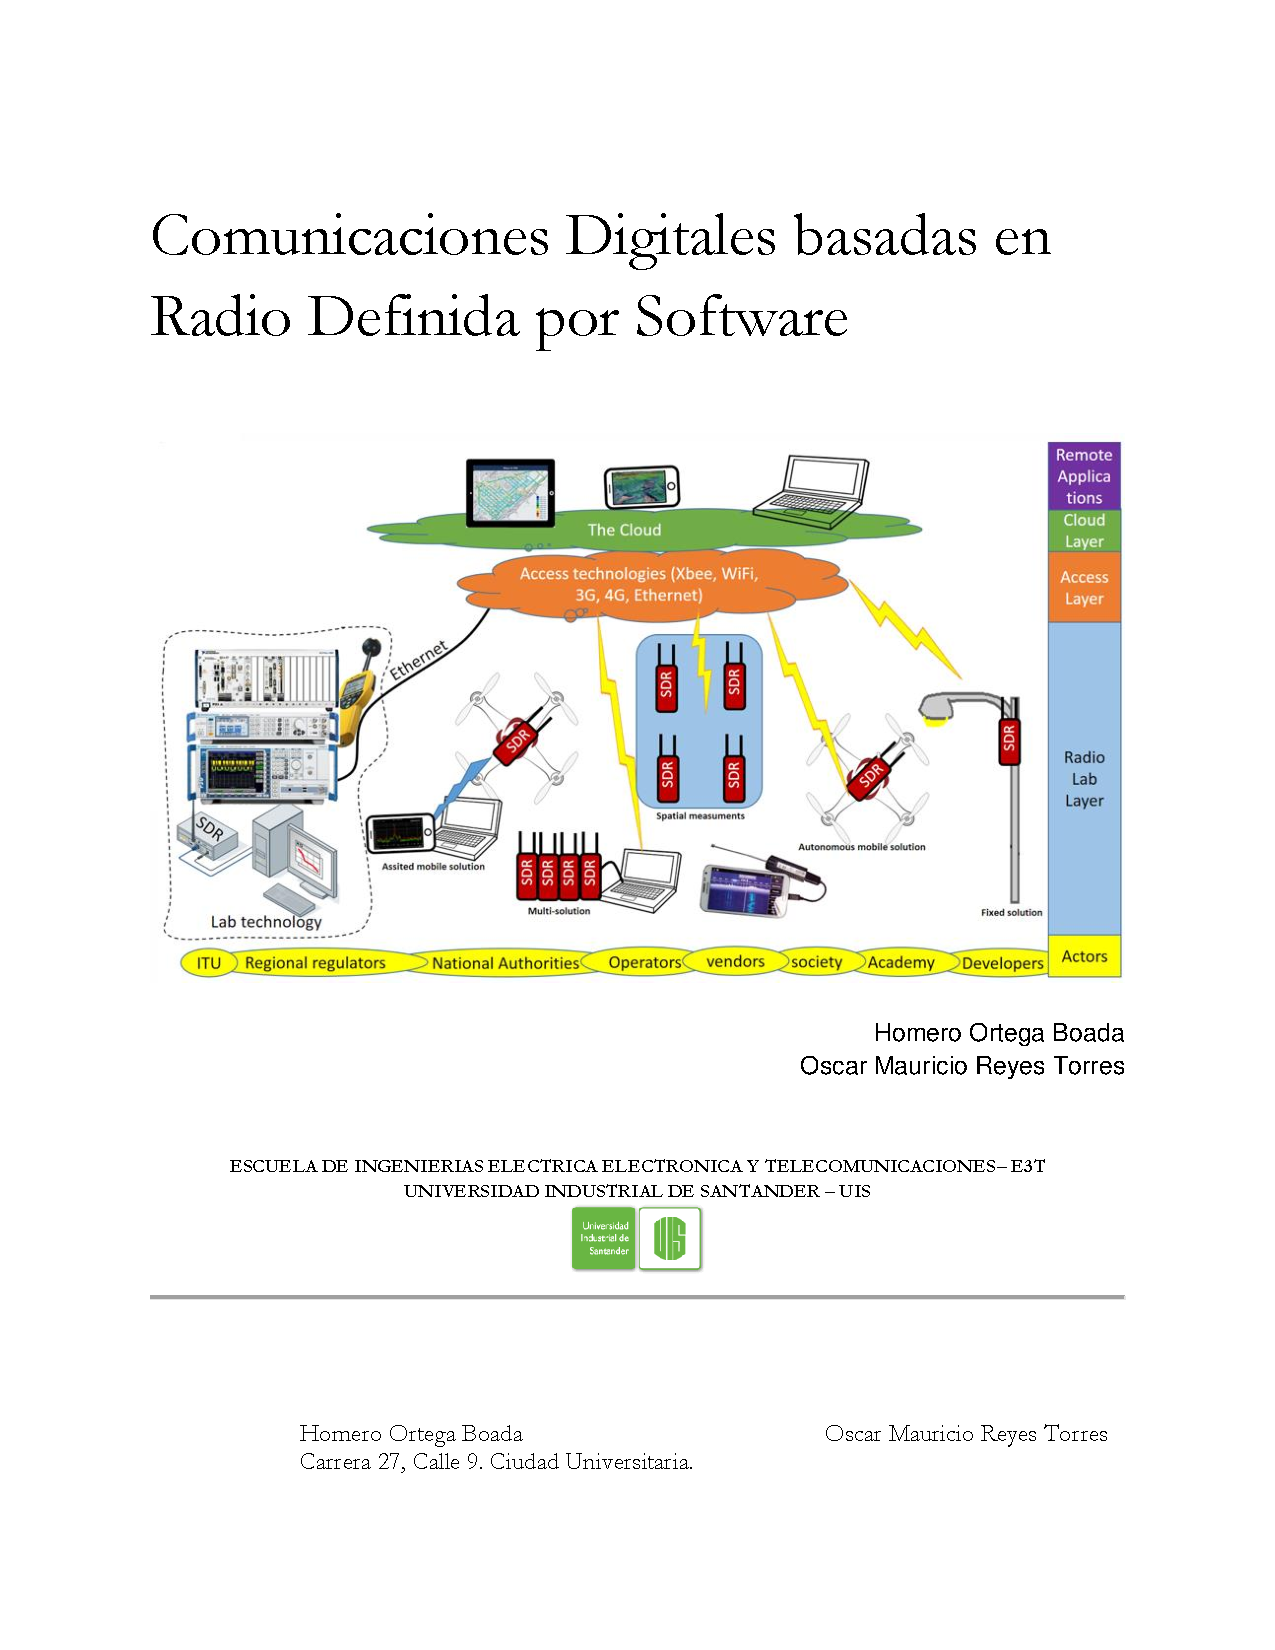
\includegraphics[trim = 20mm 19mm 19mm 16mm, clip,width=\textwidth]{Imagenes/Portada}%trim recorta izquierda abajo derecha arriba
\par
\end{center}

%%%%%%%%%%%%%%%%%%%%%%%%%%%%%%%%%%%
%%%%%%%%%%%%%		Contraportada 	%%%%%%%%%%%
\newpage
\begin{center}
\pagestyle{plain}
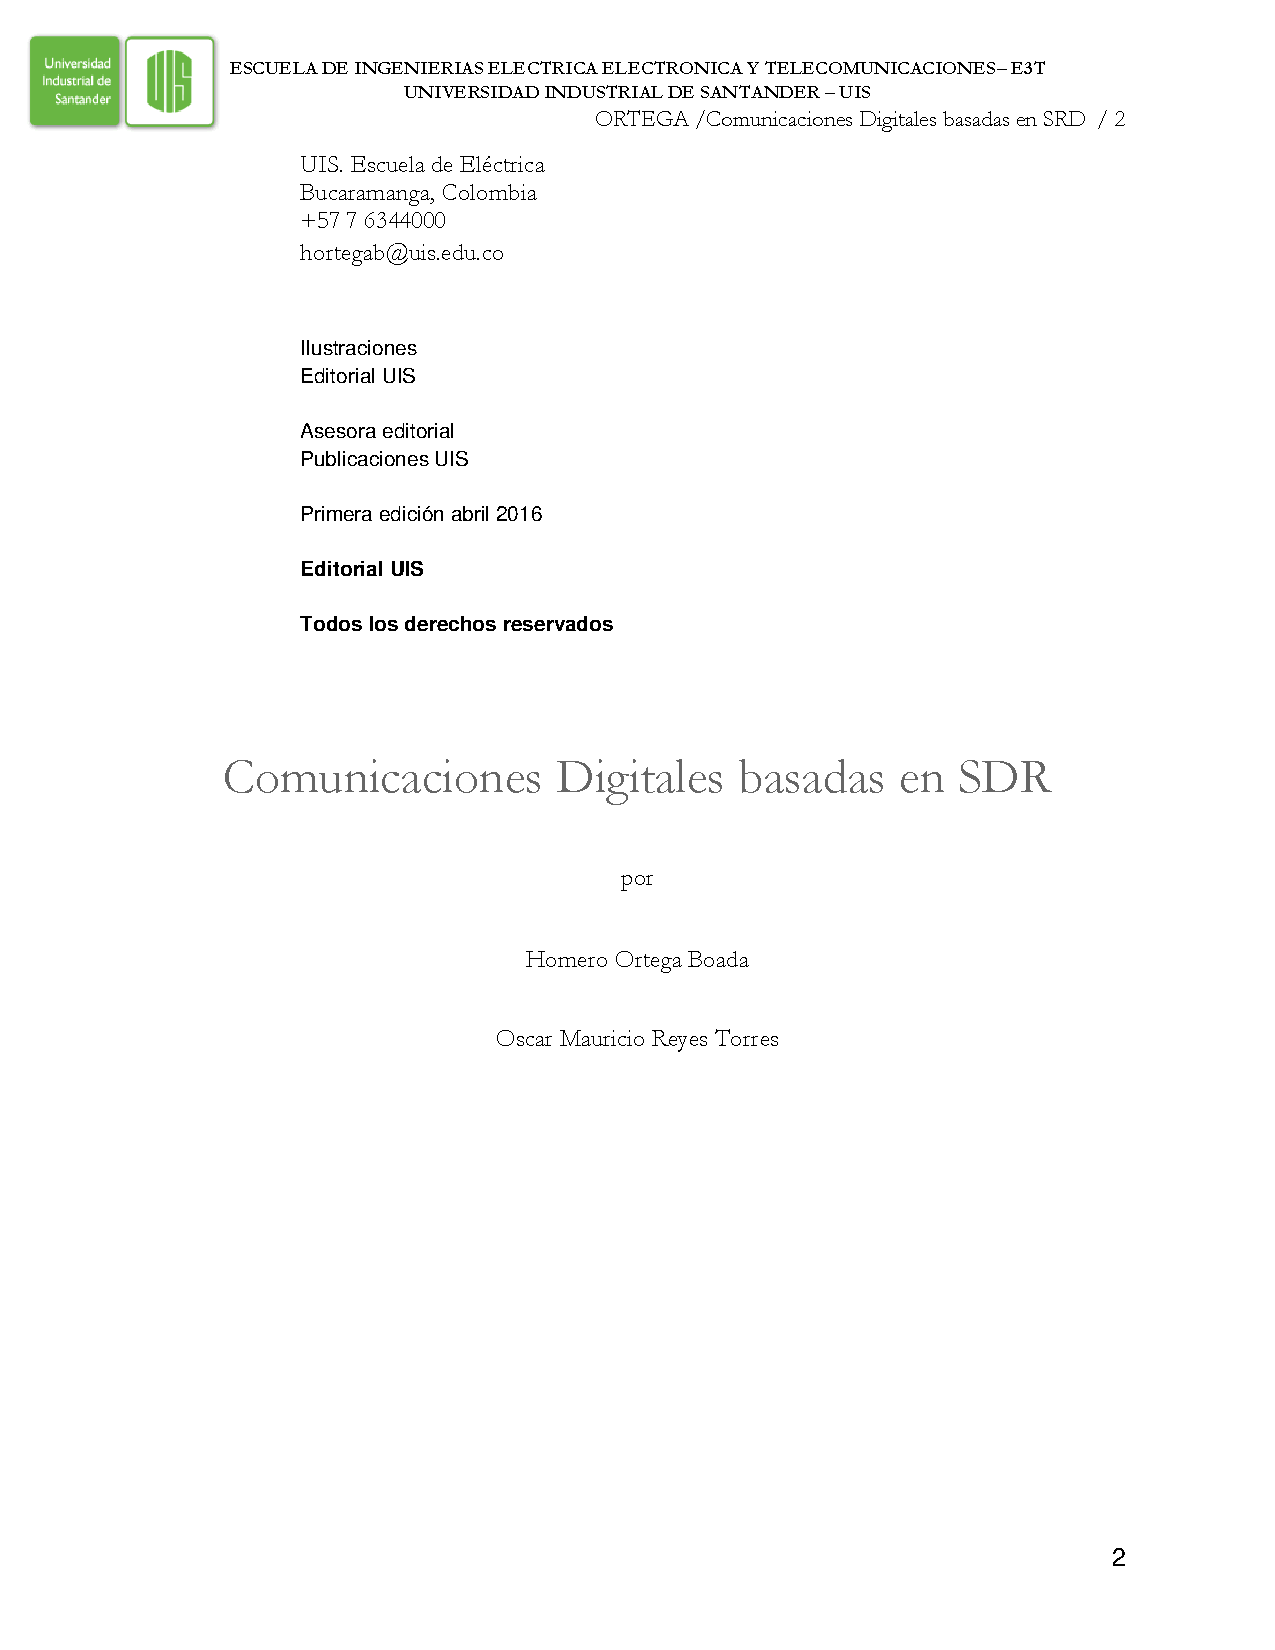
\includegraphics[trim = 2mm 19mm 19mm 1mm, clip,width=\textwidth]{Imagenes/Contraportada}%trim recorta izquierda abajo derecha arriba
\par
\end{center}

%%%%%%%%%%%%%%%%%%%%%%%%%%%%%%%%%%%
%%%%%%%%%%%%%	AUTORES	%%%%%%%%%%%
\newpage
\begin{center}
\pagestyle{plain}
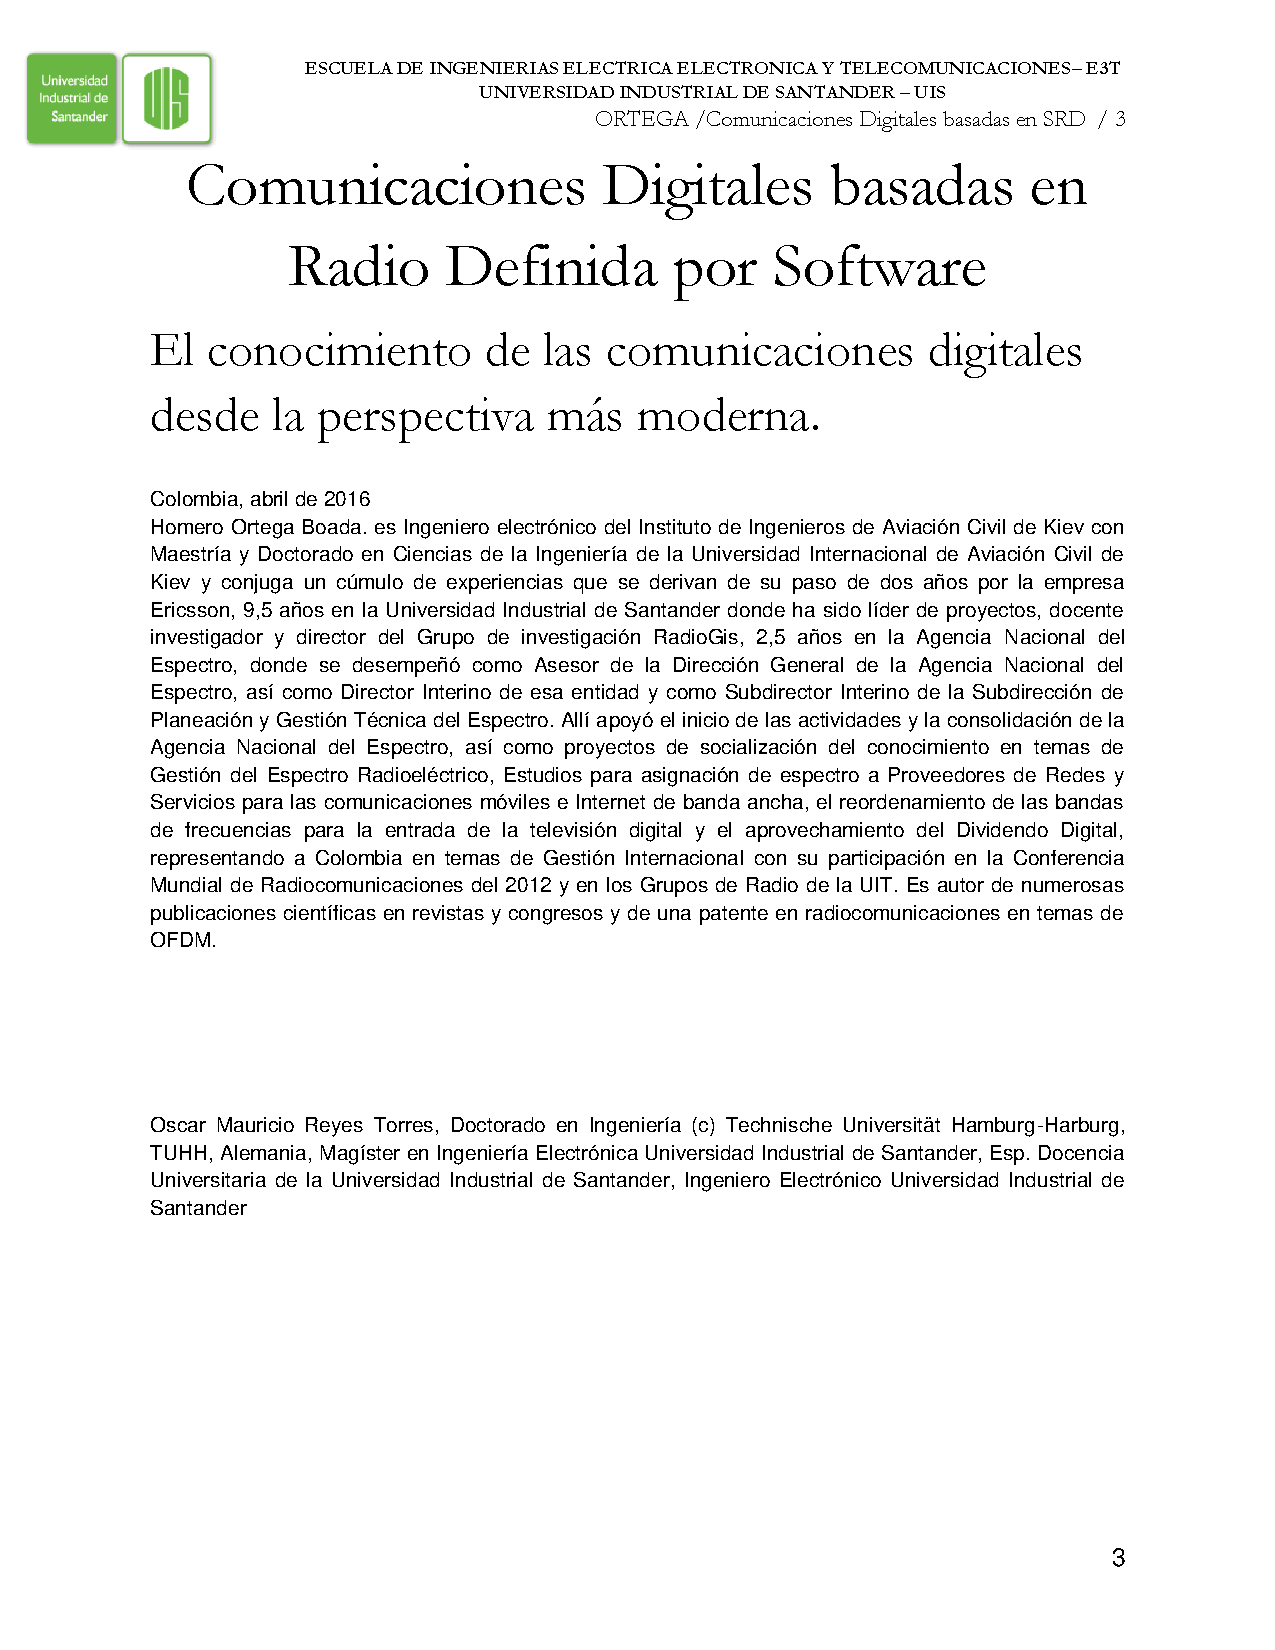
\includegraphics[trim = 1mm 19mm 19mm 1mm, clip,width=\textwidth]{Imagenes/Autores}%trim recorta izquierda abajo derecha arriba
\par
\end{center}
\tableofcontents
\listoffigures
\listoftables
%%%% INTRODUCCION
\chapter*{\centering INTRODUCCIÓN}
\markright{INTRODUCCION}
\addcontentsline{toc}{chapter}{INTRODUCCIÓN}%para que aparezca en la tabla de contenidos
\label{Cap:Introduccion}


\markright{INTRODUCCIÓN}

Las comunicaciones han sido durante todos los tiempos la clave para el desarrollo social de la humanidad. Desde las señales de humo como medio de comunicación, pasando por la invención de la rueda, la imprenta, hasta llegar al teléfono, la televisión y el Internet. Cada uno de esos avances ha impulsado un nuevo paso del hombre por las diferentes etapas de desarrollo social como la sociedad agraria, la sociedad industrial y la sociedad de la información. Por eso, varios autores aseguran que la historia de las comunicaciones es la historia de las revoluciones sociales. El nuevo paradigma es hoy la convergencia de las comunicaciones, es decir, la unión de: los medios de comunicación; la robótica; las redes de sensores para medir diferentes variables y fenómenos; el procesamiento inteligente de la información para la toma de decisiones; la informática; elementos normativos, de negocios y sociales. Esto al servicio de las actividades humanas como por ejemplo: la medicina, la industria y la conservación del medio ambiente. El término que aglutina todos esos componentes es hoy “\textit{Tecnologías de la Información y las Comunicaciones} (TIC)”. La ola de fusiones estratégicas a nivel empresarial así como los acontecimientos mundiales que se relacionan con la globalización del mundo son consecuencia de las TIC.
\\

El auge de los sistemas inalámbricos y el desarrollo de más y mejores servicios de última generación en comunicaciones exige a los ingenieros electrónicos % \OR sólo a los ing electrònicos?
estar a la vanguardia de estos avances científicos y tecnológicos. Ante esta realidad, este curso busca crear las competencias necesarias para que los ingenieros electrónicos egresados de la UIS 
% \OR resulta confusa la idea. El libro se dirige EGRESADOS? ¿sólo de la UIS? ¿sólo ing. electrónicos?
puedan fácilmente comprender las telecomunicaciones no sólo al nivel que requieren los operadores y proveedores de tecnologías, sino también al nivel científico. Abordar todos los temas de las comunicaciones en este curso % \OR ¿este libro en lugar de este curso?
es prácticamente imposible, pero sí se enfatiza en las competencias clave para lograr que los ingenieros de la UIS tengan una ventaja teórico-práctica frente a otros egresados para facilitar su participación en la demanda nacional e internacional en el campo de las comunicaciones. % \OR de nuevo, no considero apropiado el énfasis en que el libro se dirija sólo a ingenieros de la UIS.
Son temas de estudio de este curso: 
% \OR de nuevo: curso o libro?
los sistemas de comunicaciones digitales, analizando diferentes sistemas de modulación digital pasobanda y bandabase actuales y profundizando en las técnicas de acceso al medio más importantes hoy en día. De igual forma se estudian diversas aplicaciones de uso actual, sus principios y fundamentos necesarios para comprenderlas y analizarlas. Se hace uso de la programación de sistemas basados en SDR usando GRC y USRP como enfoque práctico de estos temas.
% \OR el glosario debería ser anterior al uso de siglas. En todo caso, es recomendable escribir su significado, al menos la primera vez que se usan.
Aunque se abordan muy débilmente otros temas relevantes como planeación de redes, mercados de las TIC, normativa y gestión del espectro, puede decirse que con este curso % \OR curso o libro?
el estudiante habrá desarrollado las competencias que mayor esfuerzo intelectual y mayor acompañamiento requieren, lo cual habrá pavimentado el escabroso camino teórico-práctico para poder avanzar de manera más cómoda en la construcción de las competencias que demanda el mercado.\\ % \OR este último párrafo, y en general la introducción se pueden revisar una vez el libro esté concluido para asegurar su coherencia y consistencia.

Si nos preguntaran en qué se diferencia este libro de todos los demás, la respuesta estaría en los siguientes puntos:\\ 

\begin{itemize}
	\item [$\bullet$]  Combina la enseñanza de las comunicaciones con la de GNU Radio.
	\item [$\bullet$] Ha sido escrito como parte de un proceso real de enseñanza, de modo que está probado en varias generaciones de estudiantes, ha crecido con ellas.
	\item [$\bullet$] Está orientado al desarrollo de competencias mediante prácticas de laboratorio.
	\item [$\bullet$] Se orienta hacia una enseñanza problematizada, de modo que para cada tema se propone un problema a resolver, se analizan sus causas y se presenta el tema como la solución a ese problema.
	\item [$\bullet$] Se usa una enseñanza siempre basada en modelos de capas.
\end{itemize}

\chapter{ Antecedentes}
\markright{CAPITULO1}
\label{Cap:cAPITULO}
\section{Instrucciones iniciales}

\subsection{El sitio web del libro}
En el sitio web del libro se ofrece todo tipo de materiales que pueden estar sujetos a actualizaciones. La dirección del sitio web del libro es la siguiente: 
% \OR qué son estas citas??
\cite{USRP} \cite{Harris2001} 

   \begin{center}
    \url{https://sites.google.com/saber.uis.edu.co/comdig} 
   \end{center}

Los materiales incluidos son los siguientes:
\begin{itemize}
    \item  Librerías desarrolladas.
    \item   Una aplicación Android.
    \item   Materiales de laboratorio.
	\item   Flujogramas.
	\item  Instrucciones de instalación del software usado.
	\item  Configuraciones.
\end{itemize}

\subsection{Los primeros pasos} % \OR pero es un solo paso???
\begin{itemize}
\item  \textbf{Primer paso:} Instalación de GNU Radio. Es importante que cada estudiante tenga instalado GNU Radio en su computador. En el sitio web del libro se tienen unas instrucciones que son actualizadas en la medida en que ese proceso pueda estar cambiando. Esta es la dirección directa:
\begin{center}
\url{https://sites.google.com/saber.uis.edu.co/comdig/manual} 
\end{center}
\end{itemize}


\section{Términos y siglas}
Se han adoptado las siglas en inglés, ya que  casi todo el material sobre el tema está en inglés, de esta manera se evita confundir al lector y más bien acercarlo al mundo real.

\begin{itemize}
	\item  \textbf{MS/s:}  del inglés Mega samples per second. Se refiere a una frecuencia de muestreo en mega muestras por segundo. 
	\item   Conversión análoga/digital o digital/análoga.
	\item  \textbf{Imágenes:}  se refiere a la manera en que se instala el software (drivers o UHD) a los equipos USRP. Las imágenes son el tipo de software que basta con copiarlo a una memoria como una SD para que quede instalado como parte del equipo.
	\item   \textbf{GRC:} GNU Radio Companion 
	\item   \textbf{USRP:} Universal Software Radio Peripheral: periférico universal de radio definido por software
	\item  \textbf{clock generation and synchronization}
	\item  \textbf{FPGA:} Sirve de interfaz entre todos los elementos esenciales del USRP: el puerto hacia el PC, los conversores de subida (DUC), los de bajada (DDC), los transmisores separados por DAC, los receptores separados por ADC (ver Juan José Murillo Fuentes, pág 20)
	\item  \textbf{ADC:} Conversor Dital Análogo, del inglés Analog to Digital Converter. En el caso de los USRP, un ADC comienza por  muestrear la señal banda base (cuando FI=0) que entrega el RF Front End, para luego convertirla en digital. El ADC tiene una frecuencia de muestreo bien definida, por ejemplo para el USRP1 es de 128 MS/s y además usa 14 bits/muestra. Hay dos veces más ADC que transmisores, con el fin de que se tenga la posibilidad de manejar en esta etapa señales complejas, compuestas por el parar: señal I y señal Q.  
	
	\item  \textbf{DAC:} Conversor Análogo Digital, del inglés, Digital to Analog Converter. En el cso de los USRPs, un DAC lo que hace es convertir a continua la señal bandabase (cuando FI=0)  que se ha de entregar al RF Front End. En el USRP1 la frecuencia de muestreo del DAC es 64 MS/s. otro dato importante es que usa 12 bits/muestra. Sobre el número de DACs aplica lo mismo que para ADCs. 
	\item  \textbf{DDC:} Se trata de la circuitería que, complementada con los  ADC, permite mover el espectro de la señal recibida desde altas frecuencias hasta ubicarla en bandabase y ya digitalizada, para lo cual usa una frecuencia de muestreo fija. Pero antes de ser entrega al computador, esta señal pasa por un diezmador que tiene como fin adaptar la frecuencia de muestreo fija a la frecuencia de muestreo que el programador desea configurar para la señal que entra al computador. Lo curioso es que el factor de diezmado solo puede ser un número tipo 8, 16,32, 64, 128, etc. Por esta razón se recomienda que programador redondee la frecuencia de muestreo que desea a un valor que sea potencia de dos si no quiere que el diezmador solo realice el mejor esfuerzo en producir la frecuencia de muestreo deseada por el programador. 
	\item  \textbf{DUC:}  El PC entrega una señal a la frecuencia de muestreo de Nyquist o superior, pero debe ser llevada a la frecuencia de muestreo que usa el DAC, que para el USRP1 es 64 MS/s 
	\item  \textbf{Power regulation }
	\item  \textbf{MS:} Mobile Station: es el términos usado por la UIT para referirse a los terminales de los usuarios, lo que en Colombia la gente conoce como celulares. Se le llama así, pues un terminal móvil puede ser más que un teléfono, puede ser también un computador, una tablet y porqué no un drone una nevera y en fìn cualquier cosa, como se reconoce en temas de Internet de las Cosas (IoT, de Internet of Things). En nuestros flujogramas, el MS es un bloque jerárquico que genera una señal aleatoria con modulación bandabase basada en la constelación que nosotros le programemos.
	\item   \textbf{TDM:} Time Division Multiplexing.
	\item  \textbf{TDMA:} Time Division Multiaccess.
	\item  \textbf{FDM:} Frequency Division Multiplexing.
	\item  \textbf{FDMA:} Frequency Division Multiaccess.
	\item  \textbf{CDM:} Code Division Multiplexing.
	\item  \textbf{CDMA:} Code Division Multi Access.
	\item  \textbf{OFDM:} Orthogonal Frequency Division Multiplexing.
	\item  \textbf{OFDMA:} Orthogonal Frequency Division Multi access.
	\item  \textbf{PN code:}  Pseudo Noise Code. Se refiere a los códigos de pseudo ruido usualmente usados en Spread Spectrum.
	\item  \textbf{ERE:} Espectro radioeléctrico.
	\item  \textbf{t-s:} time slot, es una celda de tiempo usada en TDM.
\end{itemize}


\section{Variables comúnmente usadas en los materiales que acompañan a este libro}

Significados de ciertas letras:

\begin{itemize}
	\item  \textbf{S:} se usa la S en mayúscula para indicar “Sample” o muestra. Se dejó así debido a que esa práctica está extendida en los manuales de los USRP y en los materiales que se encuentran en Internet que usualmente están inglés.
	\item  \textbf{s:} Se usa la s en minúscula para indicar “symbol”.
	\item  \textbf{B:} Byte (cuando se refiere a unidad de medición).
	\item  \textbf{b:} bit
\end{itemize}

Para señales en el canal o bloques de la capa de precanal:

\begin{itemize}
	\item  \textbf{Fc (Hz):} frecuencia de la portadora de radiofrecuencias, la frecuencia central de la banda de frecuencias asignada para la comunicación.
	\item  \textbf{B:} Es el ancho de banda pasobandas del canal inalámbrico. Se refiere a la banda útil del espectro radioeléctrico (ERE) que se puede usar para una comunicación dada.
	\item  \textbf{BW:} Ancho de banda bandabase. A diferencia de B, este valor aplica para la envolvente compleja de la señal útil que viaja por el ERE.
	\item  \textbf{B\_eFM:} El ancho de banda de una emisora FM.
	\item  \textbf{Kd:}  Coeficiente de decimación que aplica el bloque decimador que hay internamente, en el USRP.
	\item  \textbf{Ki:}  Coeficiente de interpolación que aplica el bloque interpolador que hay internamente en el USRP.
	\item  \textbf{Kd\_d:}  Es el coeficiente de decimación deseado, es decir, el que resultaría si el USRP pudiese manejar cualquier coeficiente de decimación. Sirve como insumo para obtener $K_d$.
	\item  \textbf{Kd\_rx, o Kd\_tx:} Se usan cuando se requiere diferenciar entre el coeficiente de decimación usado en recepción y el usado en transmisión.
	\item  \textbf{Samp\_rate (Hz):} Es la frecuencia de muestreo que maneja el USRP, luego es la frecuencia de muestreo de la envolvente compleja que viaja por el cabe Ethernet. 
	\item  \textbf{Samp\_rate\_d (Hz):} Es la frecuencia de muestreo de la señal de la envolvente compleja  que desearíamos entregar al USRP, pues es la que se obtiene teóricamente.
	\item  \textbf{Samp\_rate\_dac (MSps):} Es la frecuencia de muestreo que usa el ADC ubicado internamente en la tarjeta hija de recepción del USRP. Es igual a 100 MSs para el NI-USRP 2920
	\item   \textbf{Samp\_rate\_adc (MSps):} Es la frecuencia de muestreo que usa el DAC ubicado internamente en la tarjeta hija de transmisión del USRP. . Es igual a 400 MSs para el NI-USRP 2920. 
	\item  \textbf{Samp\_rate\_rx (Hz):} Es igual que samp-rate, solo que se usa cuando queremos diferenciar este parámetro de la frecuencia de muestreo usada en transmisión. De modo que es la frecuencia de muestreo de la señal de la envolvente compleja  que entregamos al USRP Sink. 
	\item  \textbf{Samp\_rate\_tx (Hz):} De manera similar a samp-rate-rx, esta es la frecuencia de muestreo de la señal de la envolvente compleja  que recibimos del USRP Source.
	\item  \textbf{Sps: (samples per symbol)}  Es el número de muestras que lleva un símbolo de la envolvente compleja que pasa al canal.
	\item  \textbf{N\_Lob\_p\_B:}Número de lóbulos del espectro de una señal digital, en el ancho de banda B. El lóbulo del medio, por tener doble ancho, se cuenta por dos. Usualmente es igual a Sps
	\item  \textbf{ntaps:} Es el número de componentes que tiene la respuesta al impulso del filtro FIR usado.
	\item  \textbf{rcc\_taps:}  Son lo taps, es decir las componentes de la respuesta al impulso, para un filtro Root Raid Cosine.
	\item  \textbf{rolloff:} Es el parámetro esencial de un Filtro Coseno Alzado. También le llaman alpha o Excess Bandwidth. 
	\item  \textbf{W (Hz):} Ancho de banda de Nyquist o del criterio de Nyquist para ISI.
	\item  \textbf{SymTune:}  Sintonización de los símbolos que entran al demodulador M-PAM al momento de armar los paquetes de bits que componen cada muestra del mensaje. Lo que se hace es retrasar en el valor SymTune los símbolos hasta que sean reconocidos correctamente por el demodulador.
	\item   \textbf{NodB (dB):} Es la altura de la PSD del ruido blanco, conocido como $N_o$.
	\item  \textbf{DelayAcc:} Retardo a introducir al Filtro de Acoplamiento con acumulador para lograr el mejor desempeño posible.
	\item  \textbf{TimingDelay:} Es el tiempo (en número de muestras) de retardo que debe ser introducido a la señal que llega al muestreador del receptor con el fin de seleccionar el mejor instante de muestreo, aquel en el que el diagrama de ojo está más abierto.
	\item  \textbf{Ch\_Jitter:} Sirve para varia el valor Epsilon del bloque Channel Model de modo que el canal produzca una inestabilidad del reloj o Jitter variable.
	\item  \textbf{Ch\_Frec\_offset:} Permite configurar canal para que produzca desfases de frecuencia.
\end{itemize}

Para las señales fuente:

\begin{itemize}
	\item  \textbf{Samp\_rate\_audio (Hz):}  Es la frecuencia de muestreo de la señal mensaje de audio, que en este caso es de audio. Esto para diferenciarla de samp-rate que la estaremos usando para el USRP.
	\item  \textbf{NbpS:}  (Number of bits per sample) es el número de bits que representan a cada muestra del mensaje.
	\item   \textbf{NivelesQ:}  Número de niveles de cuantificación de la señal mensaje cuantificada.
	\item  \textbf{Vp:} Amplitud máxima que puede alcanzar la señal mensaje antes de ser cuantificada.		
\end{itemize}

Para señales binarias:

\begin{itemize}
	\item  \textbf{Rb (bps):} Rata de bits.
	\item  \textbf{DelayBits:} Es el retraso que habría que introducir a los bits transmitidos para que puedan ser comparados en una misma escala de tiempo con los recibidos.
	\item  \textbf{NBpCode:} Número de bytes por código, cuando se usan codificadores a los cuales se le inyecta un código a una carga útil en bytes, como es el caso del bloque b-PCM-EncoderBb
	\item  \textbf{SpB:} Muestras por Byte. Cuando se usa un codificador que introduce a cada Byte bits redundantes, entonces se usa este parámetro que sirve para conocer qué tanto se pueda alterar la frecuencia de muestreo con esa codificación.
	\item   \textbf{Ri}  Rata de bits útil. En los casos en que se usa codificador.
\end{itemize}

Para señales moduladas:

\begin{itemize}
	\item  \textbf{Constelación:} Representa la tabla de verdad de la modulación usada.
	\item  \textbf{MiconstellationObject:} Es una constelación, pero hecha bajo unas normas comunes para una familia de bloques GNU Radio, como por ejemplo el bloque Constellation Decoder.
	\item  \textbf{M:} Orden de la modulación usada.
	\item  \textbf{Rs (Baud):}Rata de símbolos. Rs: Es la rata de símbolos útil que se entrega al canal. No incluye símbolos usados en señalización, sincronismo o alineamiento de tramas.
	\item  \textbf{Ts:} Duración de un símbolo.
	\item  \textbf{Tsamp:} Periodo de muestreo.
	\item  \textbf{Bps: (Bits per symbol)}Número de bits que representan cada símbolo de la señal modulada.
	\item  \textbf{SymDelay:} Symbol delay. Es el retraso que habría que introducir a los bits transmitidos para que puedan ser comparados en una misma escala de tiempo con los recibidos.

\end{itemize}

Capas de multiplexado:
\begin{itemize}
	\item  \textbf{Rsu:} Es la rata de símbolos de cada usuario que corre por el canal, cuando el canal se usa para enviar información de varios usuarios, como cuando se usa el multiplexado.
	\item  \textbf{Rbu:} Rata de bits por usuario, cuando hay màs de un usuario en el sistema de comunicación, como por ejemplo cuando se usa multiplexado.
	\item  \textbf{$Nspt_s:$} Número de símbolos por time slot. Es el número de símbolos que un usuario pone en cada ventana de tiempo (time-slot) que ocupa en la trama multitplexada.
	\item  \textbf{SymSysDelay o MuxDelayComp:} Es retardo que sufre la señal de la información al viajar por todo el sistema hasta llegar al punto de destino. Sirve para introducir un retardo a la señal transmitida a la hora de compararla con la recibida.
	\item  \textbf{ChipSysDelay:} Es el equivalente a SymSysDelay pero dado en número de chips, cuando se usa DS-SS. Es demasiado útil en el bloque b-de-ds-spreadspect-cc ya que el código que se va a aplicar debe ser previamente retrasado en el valor para que funcione correctamente el de-ensanchamiento.   
	\item  \textbf{SF:} Spreading Factor. Es el número de veces que el espectro se ensancha. Es la relación entre el ancho de banda que ocupa la señal ensanchada con respecto al que ocuparía sin la técnica DSSS.
	\item  \textbf{Rch:} Rata de chips
	\item  \textbf{Spch:} Samples per chip. Es el número de muestras asignadas a cada chip.
	\item  \textbf{C-PN:} Almacena un vector de un código de pseudo ruido.
	\item  \textbf{Spch:} Samples per chip. Es el número de muestras por chip que se usa cuando una señal ensanchada con DS-SS se entrega a un USRP. Es el equivalente a sps, solo que en DS-SS no se envían símbolos, sino chips.
	\item  \textbf{Nu:} Número de usuarios 
	\item  \textbf{Rs\_subchannel:} Se refiere a la rata símbolos que lleva cada subcanal para el caso de señales multiplexadas, donde cada canal aporta una rata de símbolos, pero la señal multiplexada lleva la suma de las ratas de símbolos de todos los subcanales.
	\item  \textbf{Us:} Usuario.
\end{itemize}


Para la instrumentación:

\begin{itemize}
	\item  \textbf{Tmax\_scope (seg):} Es la duración de la ventana que se gráfica en el osciloscopio.
	\item  \textbf{Nscope\_span:} Es el número de símbolos que se desean mostrar en un osciloscopio.
\end{itemize}

\section{Señales y Sistemas continuos en el dominio del tiempo}

\subsection{Señales senoidales}

Las señales senoidales son quizá las más conocidas y las más importante sobre todo porque son la base para la Teoría de Fourier sobre la cual se apoyan las radiocomunicaciones. Es quizá por esa razón que los sistemas de comunicaciones se orientan a transmitir y a recibir señales senoidales. Así, una antena transmisora no hace otra cosa que recibir una señal senoidal eléctrica para emitirla en forma de una onda senoidal electromagnética. Lo contrario hace la antena receptora.\\

Los siguientes son los aspectos más relevantes a tener en cuenta sobre las señales senoidales:

\begin{itemize}
\item  una señal senoidal pura puede ser representada matemáticamente como.

 \begin{equation}  \label{eu_eqn}
 c(t)=A\cos(2 \pi f t + \phi)
 \end{equation}

\item  Pero además, con el fin de poder llevar información sobre la onda, es posible hacer variar uno de los parámetros, con lo cual tenemos 3 posibles casos:

   \begin{itemize}
   \item  Varia sola la amplitud de la senoidal. 
   		\begin{equation} \label{equ_uno}
   			c(t)=A(t)\cos(2 \pi f t+ \phi)
    	\end{equation}
   \item  Varía solo la frecuencia de la senoidadl
         \begin{equation} \label{equ_dos}
         	c(t)=A\cos(2 \pi f(t) t+ \phi)
         \end{equation}
   \item  Varía solo la fase de la senoidal.
         \begin{equation} \label{equ_tres}
         	c(t)=A \cos(2 \pi f t+\phi(t))
         \end{equation} 
\item  Una señal senoidal puede ser vista como una combinación lineal de dos señales exponenciales complejas, pues:
\begin{equation} \label{equ_cuartro}
	\cos(t)=\frac{e^{jt}+e^{-jt}}{2} 
\end{equation}

   \end{itemize}
\end{itemize}

%%%%%%%%%%%%%%%%%%

\subsection{La respuesta al impulso y la convolución}

La respuesta al impulso y la convolución son temas que aplican a los sistemas Lineales e Invariantes en el Tiempo (LIT). En realidad esos sistemas no son tan comunes en el mundo en el mundo real, de manera que se trata de más bien de casos ideales, pero en muchísimos casos, un sistema que varía en el tiempo puede ser visto como invariante durante lapsos de tiempo que pueden ser muy pequeños o muy grandes. Este libro no busca explicar detalladamente la teoría de sistemas LIT, solo resumir los conceptos necesarios para los propósitos del libro.
\subsubsection{Conceptos básicos}
El siguiente en un resumen de conceptos mínimos sobre este tema:
\begin{itemize} 
\item En la teoría de sistemas LIT es importante considerar el sistema más sencillo, con una entrada que usualmente identificaremos como $x(t)$ y una salida $y(t)$.
\item  Vamos a considerar también que para una entrada $x_1(t)$ la salida del sistema es $y_1(t)$; para una entrada $x_2(t)$ la salida es $y_2(t)$ y así sucesivamente.  
\item El sistema es lineal si se cumplen las siguientes condiciones:
    \begin{itemize}
    \item  Se cumple la propiedad de aditividad que consiste en que si la entrada de sistema es $x_3(t)=x_1(t)+x_2(t) $ la salida del sistema es $ y_3(t)=y_1(t)+y_2(t)$
    \item Se cumple la propiedad de escalamiento y homogeneidad que consiste en que si la entrada es $x_1(t)=a x(t)$, donde $a$ es una constante, la salida será $y_1(t)=ay(t)$
    Se infiere que también se cumple la propiedad de superposición que dice que si la entrada es:
    \begin{center}
    $x(t)=a_1x_1(t)+a_2x_2(t)+a_3x_3(t)+ ...$
    \end{center}
    la salida es
    \begin{center}
    $y(t)=a_1y_1(t)+a_2y_2(t)+a_3y_3(t)+ ...$
    \end{center}
    \end{itemize}
\item El sistema es invariante si ante una entrada $x_1(t)=x(t-T_0)$ la salida es $y_1(t)=y(t-T_0)$, donde $T_0$ es un valor de tiempo
\item Un sistema es LIT se se cumple a la vez que es lineal y es invariante
\item Si la entrada al sistema es la función impulso, también conocida como Delta de Dirac, la salida del sistema se conoce como la respuesta al impulso. De modo que si  $x(t)=\delta (t)$, se tine la salida $y(t)=h(t)$, donde $h(t)$ es la manera en que se representa la respuesta al impulso de un sistema LIT.

\item Todo sistema LIT puede estar completamente definido mediante su respuesta al impulso. De modo que si se conoce la entrada y la respuesta al impulso del sistema, la salida puede ser calculada mediante una operación conocida como Convolución que está dada por la siguiente expresión: 
\begin{equation} \label{hob1}
	 y(t)= \int_{-\infty}^{\infty} x(\tau)h(t-\tau)d \tau 
\end{equation}
\item La operación de convolución también se puede indicar de la siguiente manera:
\begin{equation} \label{convolucion}
	 y(t)= x(t)*h(t) 
\end{equation}

\end{itemize}


%%%%%%%%%%%%%%%%%%%%%%%%%%%%%%%%%%%%%%%%%%%%%%%|
\subsection{ La Representación en Series de Fourier}

Para los propósitos del presente libro, es importante recalcar los siguientes aspectos sobre la Representación en Series de Fourier (RSF):\\

\begin{itemize}
	\item  La señal analizada $x_{T}(t)$ es continua y periódica, con periodo igual a T segundos.
    \item  El resultado de la transformación no guarda relación con la energía total de la señal ya que lo que se transforma es solo la porción de la señal que se observa en un periodo de tiempo
    \item[$\bullet$] El espectro resulta siendo discreto, con componentes o muestras espectrales separadas entre sí en $ f_0= \frac{1}{T} $
    \item[$\bullet$] El espectro se expresa en las mismas unidades en que está expresada la señal en el tiempo. Por ejemplo, si la amplitud de la señal está dada en voltios, las muestras en el espectro estarán dadas también en voltios. 
	\item  La ecuación de análisis de la RSF es la siguiente:
		\begin{equation} \label{equ_cinco}
			 C_{k} = \dfrac{1}{T} \int\limits_{(T)} x_T (t) e^{-j2 \pi k f_0 t}				
		\end{equation} 	
\end{itemize}



\subsection{La Transformada de Fourier}

Este capítulo busca resumir sobre los aspectos relevantes de la Transformada de Fourier (TF). Vale la pena recordar que un rayo de luz de color puro es una onda con una frecuencia definida, pero nuestros ojos no ven la forma de la onda, solo ven su color. Pero también podemos distinguir diferentes colores de luz que llegan a nuestros ojos combinados en una sola señal. Eso significa que: hay al menos dos formas de ver las señales, en el dominio del tiempo y en el dominio de las frecuencias y nuestros ojos solo pueden ver en el dominio de las frecuencia. Precisamente, la TF es la herramienta teórica que permite que una señal que está expresada en el dominio del tiempo pase a ser expresada en el domino de las frecuencias. La TF no deja de ser una herramienta teórica, pero es posible realizar adaptaciones con fines prácticos. Los aspectos teóricos son los siguientes:

\begin{itemize}
	\item La señal analizada $x(t)$ no necesariamente es periódica.
	\item Se aplica a esa señal el mismo concepto de la RSF pero en las siguientes condiciones:
	\begin{itemize}
		\item  Se considera que el periodo de x(t) es infinito
		\item para $C_{k}$ no sea cero, se escala en ese periodo infinito.
		\begin{equation} \label{equ_seis}
			X(f) = \lim_{T \to \infty}  TC_{k}
		\end{equation} 
	\item Debido a este escalamiento, si la amplitud de la señal está dada en voltios, el espectro estará dado en V/Hz.
	\item Lo anterior hace que $f_0$ tienda al valor cero, por tanto, $ kf_{0}$ tiene a ser la variable continua $f$, de modo que la parte derecha de la fórmula (\ref{equ_seis}) tiende a la siguiente expresión, mejor conocida como la Ecuación de Análisis de la Transformada de Fourier, así como también se puede deducir la Ecuación de Síntetis.
	\end{itemize}
    \item La Ecuación de Análisis\\
    \begin{equation} \label{equ_ocho}
	    X(f)=\int_{-\infty}^{\infty} {x(t)e^{-j2 \pi f t}dt}
    \end{equation}

    \item La Ecuación de Síntesis\\
    \begin{equation} \label{equ_nueve}
    	x(t)=\int_{-\infty}^{\infty} {X(f)e^{j2 \pi f t}df}
    \end{equation} 

    
\end{itemize}

\subsection{La Respuesta en frecuencia en los sistemas LIT}
El siguiente es el resumen conceptual necesario sobre este tema:
\begin{itemize} 
\item Toda señal $x(t)$ del mundo físico tiene una respresentación $X(f)$ en el dominio de las frecuencias que se puede hallar mediante la TF. 
\item La respuesta al impulso $h(t)$ de un sistema LIT también tiene una representación $ H(f)$ en el dominio de las frecuencias. $H(f)$ es lo que se conoce como la respuesta en frecuencia del sistema. 
\item Como la respuesta al impulso de un sistema LIT define completamente el sistema, entoces $H(f)$ también define completamente al sistema.
\item En el domino de las frecuencias, la operación de Convoluión, representa en la fórmula \ref{convolucion} cambia a una operación de multiplicación. De modo que, si conocemos la señal entrante en el dominio de las frecuencias y la respuesta en frecuencia de un sistema LIT podemos calcular la salida en el dominio de las frecuencias de la siguiente manera:
\begin{equation} \label{multiplicacionenfrec}
	 Y(f)=X(f)H(f)				
\end{equation}

\end{itemize}
\subsection{Transformada de Fourier de algunas señales}
Para los propósitos del libro, a continuación listamos las señales de interés la TF de cada una de ellas.
\begin{itemize} 
\item La señal exponencial compleja: 
\begin{equation} \label{DFTeexp}
	 e^{j2 \pi f_0t}	\xrightarrow{TF} \delta(f-f_0)			
\end{equation}
\item Una onda coseno.
de acuerdo a la fórmula de Euler la función coseno se puede expresar en términos de funciones exponenciales complejas así:
\begin{equation} \label{DFTecos}
	 cos(t)=\frac{e^{jt}+e^{-jt}}{2}
\end{equation}
Teniendo en cuenta que la TF es  una operación lineal, se deduce que:
\begin{equation} \label{DFTecos1}
	 cos(2 \pi f_0t)	\xrightarrow{TF} \frac{1}{2} \delta(f-f_0)+\frac{1}{2} \delta(f+f_0)			
\end{equation}
\item Una onda seno.
Siguiendo la misma lógic anterior, la función seno se puede expresar en términos de funciones exponenciales complejas así:
\begin{equation} \label{DFTecos2}
	 sin(t)=\frac{e^{jt}-e^{-jt}}{2j}
\end{equation}
Por lo tanto, 
\begin{equation} \label{DFTecos3}
	 sin(2 \pi f_0t)	\xrightarrow{TF} \frac{1}{2j} \delta(f-f_0)-\frac{1}{2j} \delta(f+f_0)			
\end{equation}
\item Una señal rectangular $rect(t)$. Sea:

\begin{equation} \label{equ_rect}
rect(t)=\left\lbrace 
\begin{array}{cc}
1    & \abs{t}<1/2 \\
1/2  & \abs{t}=1/2 \\
0    & \abs{t}>1/2
\end{array}
\right\rbrace
\end{equation}

Entonces, su relación con la TF es la siguiente:
\begin{equation} \label{equ_tf_rect}
A rect(t)\xrightarrow{TF} Asinc(f)					
\end{equation}
\item Para una señal sinc se tiene la siguiente relación:
\begin{equation} \label{equ_TF_sinc}
A sinc(t)\xrightarrow{TF}  A rect(f)
\end{equation}

\end{itemize}

\subsection{La Modulación de una señal senoidal}
Bajo ciertas condiciones, una señal senoidal puede portar a una señal mensaje. Para ello, es necesario hacer que la amplitud del mensaje modifique uno de los parámetros de la señal senoidal. % \OR no es preciso.... no es sólo la amplitud!!!
El término modulación se usa en las comunicaciones para referirse al proceso de hacer que un mensaje modifique o varíe uno o más parámetros de una señal portadora. La siguiente expresión matemática refleja los parámetros que pueden ser variados por medio del mensaje:\\

\begin{equation} \label{equ_diez}
c(t)=A(t) cos[2 \pi (f_c+F(t))t+B(t)]
\end{equation} 
\subsubsection{La Modulación de Amplitud de Doble Banda Lateral}
En la modulación en amplitud de amplitud de doble banda lateral (DSB), del inglés Double Side Band, la señal mensaje $m(t)$ entra al modelo anterior como:

	\begin{equation} \label{equ_once}
		A(t)= m(t)
	\end{equation} 

Los demás parámetros variables se llevan a cero.

	\begin{equation} \label{equ_doce}
		F(t)= 0
    \end{equation}
    
    \begin{equation} \label{equ_trece}
		B(t)= 0
	\end{equation} 

De modo que se obtiene la señal modulada s(t).

	\begin{equation} \label{equ_catorce}
		s(t)=m(t)\cos(2 \pi f_ct)
	\end{equation} 

\textcolor{red}{[Falta: Oscar reyes: gráfica en el dominio del tiempo, parámetros]}

\subsubsection{La Modulación de Amplitud}
La modulación en amplitud (AM) la señal mensaje $m(t)$ entra al modelo anterior como:

	\begin{equation} \label{equ_quincex}
		A(t)= K_a[1+m(t)]
	\end{equation} 

Donde $K_a$ se conoce como coeficiente de modulación de amplitud. Los demás parámetros variables se llevan a cero.

	\begin{equation} \label{equ_dieciseisx}
		F(t)= 0
    \end{equation}
    
    \begin{equation} \label{equ_diecisitex}
		B(t)= 0
	\end{equation} 
	
De modo que se obtiene la señal modulada s(t).

	\begin{equation} \label{equ_diecioschox}
		s(t)=K_a [1+m(t)]cos(2 \pi f_ct)
	\end{equation} 

En la Figura \ref{fig:am_t} se presenta un ejemplo, donde se tiene como entrada un mensaje representado por una señal de audio y una onda senoidal que sirve como portadora. En la parte inferior se tiene el resultado de la modulación. Como puede apreciarse, se trata de la misma onda portadora, pero con variaciones de amplitud que son proporcionales a la amplitud de la señal mensaje.
\begin{figure}[h!]
	\captionsetup{justification = raggedright, singlelinecheck = false}
	\caption{Ejemplo de la modulación AM} 
	\centering
	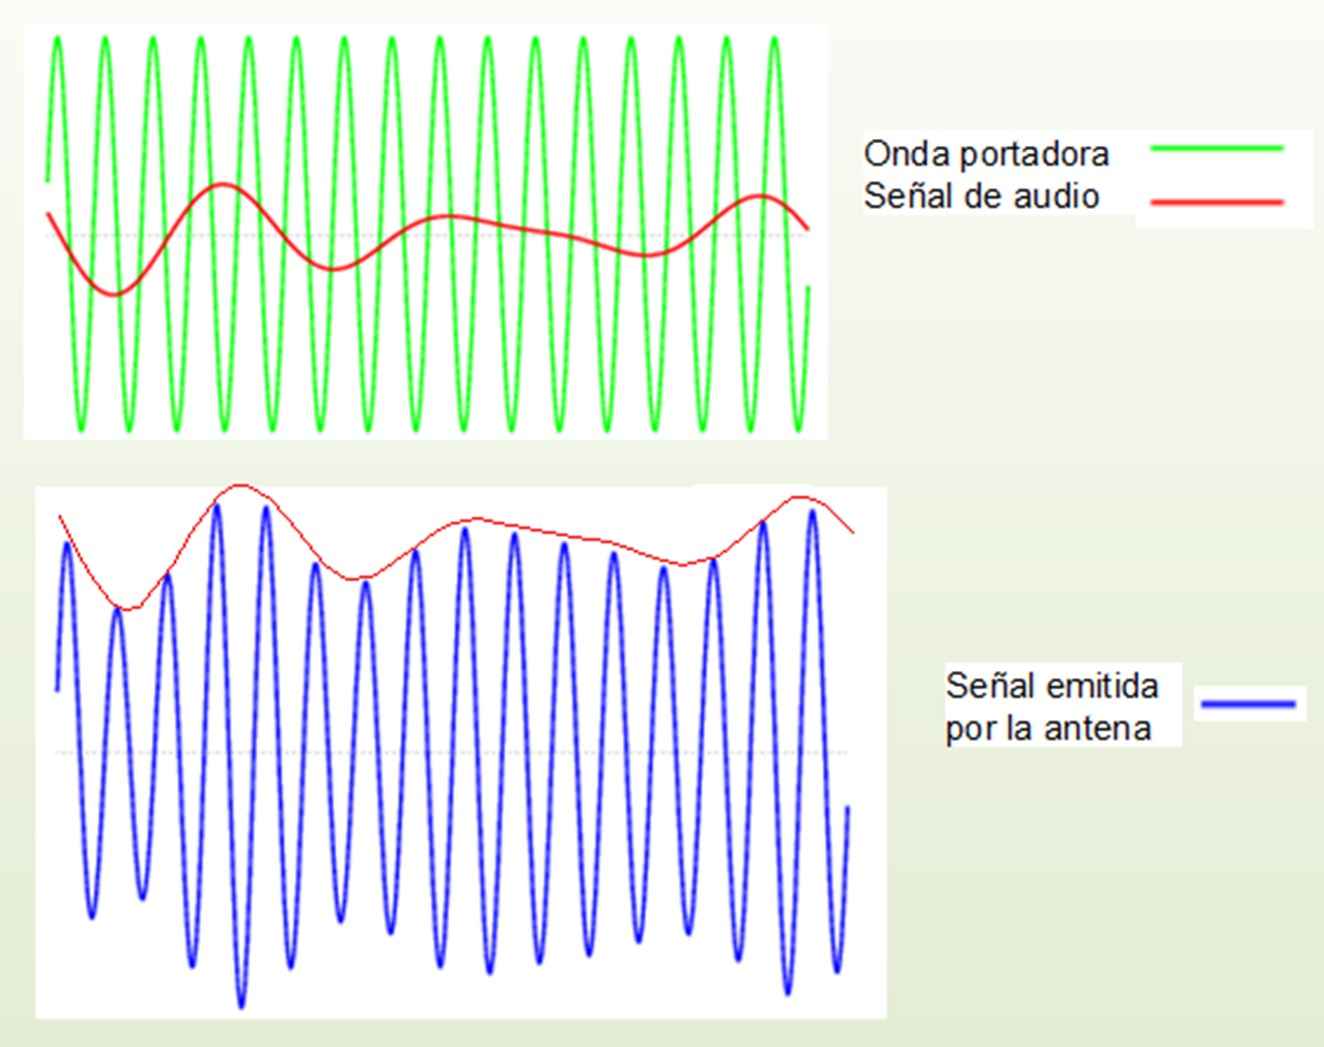
\includegraphics[scale=0.5]{Imagenes/am3.jpg}
	\label{fig:am_t}
    \captionsetup{justification=raggedright,font={scriptsize,bf,it}}
   \caption*{}
\end{figure}

\subsubsection{La Modulación de Frecuencia}
En la modulación de frecuencia (FM) el modelo anterior cambia de la siguiente manera:

\begin{equation} \label{equ_quince}
A(t)=A_c
\end{equation}

\begin{equation} \label{equ_dieciseis}
F(t)= K_f m(t)
\end{equation}

\begin{equation} \label{equ_diecisiete}
B(t)= 0
\end{equation}

Donde $K_f$ se conoce como coeficiente de modulación de frecuencia. Entonces se obtiene la señal modulada $s(t)$:

\begin{equation} \label{equ_diesiocho}
	s(t)=A_c cos[2 \pi (f_c+K_f m(t))t]
\end{equation}

Mediante algunas mejoras a la fórmula anterior se puede llegar a una expresión más conocida para la modulación FM.

\begin{equation} \label{equ_diesinueve}
s(t)=A_c cos[2 \pi f_c t + K_f \int m(t) dt]
\end{equation} 

De la expresión anterior se deduce que la Modulación FM representa también una forma de modulación de fase.

\textcolor{red}{[Falta: Oscar Reyes: gráfica en el dominio del tiempo, parámetros.]}


\subsubsection{La Modulación de Fase}
En la modulación de fase (PM) el modelo anterior cambia de la siguiente manera:

\begin{equation} \label{equ_veinte}
A(t)=A_c
\end{equation} 

\begin{equation} \label{equ_veintiuno}
F(t)= 0 
\end{equation} 

\begin{equation} \label{equ_veintidos}
B(t)= K_p m(t)
\end{equation} 

Donde $K_p$ se conoce como coeficiente de modulación de fase. Entonces se obtiene la señal modulada $s(t)$:

\begin{equation} \label{equ_veintitres}
s(t)=A_c cos[2 \pi (f_c t + K_p m(t))]
\end{equation} 

\textcolor{red}{[Falta: Oscar reyes: gráfica en el dominio del tiempo, parámetros.]}
\subsubsection{Análisis en el dominio de las frecuencias}
\textcolor{red}{[Falta: Oscar reyes: La idea es realizar una comparación entre todos los tipos de modulación en el dominio de las frecuencias. Pero si el profe Oscar tiene otra idea, tambien es aceptable, por ejemplo que ese análisis se haga por cada uno de los tipos de modulación por separado]}
% \OR para revisar desde la notación misma....

\section{Señales aleatorias}

\subsection{Planteamiento del problema}

Hasta el momento, se han visto señales teóricas o deterministicas que pueden ser presentadas por fórmulas matemáticas u otras maneras. En el mundo real las señales son casi siempre aleatorias y eso hace que los conceptos vistos anteriormente no se pueden aplicar de manera directa. Por ejemplo, si pretendemos usar el concepto estricto de la TF para observar, en el dominio de las frecuencias la voz de una persona, deberíamos esperar a que esa persona hable durante toda su vida antes de aplicarle la TF, pues esta, por definición analiza la señal en el tiempo que va desde $t = -\infty $ hasta $t = \infty $. Es claro que esto no es viable en la mayoría de las aplicaciones prácticas debido a la necesidad de resultados en tiempos más reales.\\

Del análisis anterior surge la pregunta: ¿Es posible usar herramientas de análisis como la Transformada de Fourier, los filtros, los sistemas LIT, etc, que han tenido su origen en señales determinísticas, para analizar señales del mundo real donde predomina más bien la aleatoriedad y el caos? ¿cómo hacerlo?. 

\subsection{Promedios de tiempo en señales reales}
La respuesta está en la necesidad de adaptar esos conceptos a dos posibles campos:
\begin{itemize}
    \item La Teoría de señales aleatorias. La idea consiste en que si bien las señales son aleatorias, varios parámetros pueden ser vistos como determinísticos, al menos dentro de ciertos límites. Por ejemplo la media de una señal, la desviación estándar, la potencia promedio, la distribución de la potencia promedio en el dominio de las frecuencias, los cuales se pueden calcular de manera aproximada al observar el comportamiento de la señal durante un tiempo tan corto o tan grande como tan pequeña o grande sea la exactitud deseada.
    \item La Teoría de procesos estocásticos. puede ser visto como una mayor generalización de la teoría se señales aleatorias, cuando la cuestión no se trata de analizar una sola señal sino un grupo de ellas. Por ejemplo, supongamos que hemos reunido las señales de voz de muchas personas diferentes para probar cómo se comportan al pasar por un sistema. El promedio de esas señales es otra señal que varía en el tiempo, pero que tiene un comportamiento más predecible.
\end{itemize}

En este capítulo solo hablaremos de la Teoría de señales aleatorias. Supongamos que en el problema en que usted trabaja solo se cuenta con una señal aleatoria, debido a las especificidades de ese problema. Es claro que esa señal tiene una media y por lo tanto todos esos parámetros que se derivan de la media, como la media cuadrática, la varianza, la desviación estándar, etc. Incluso la función de distribución de probabilidad. En este caso, el concepto que se usa se conoce como Promedios de Tiempo. Los cálculos son similares a los que se realizan con una Variable Aleatoria, la diferencia está esa variable tiene un resultado en cada instante de tiempo y que hay infinitos instantes de tiempo, ya que el tiempo es continuo. \\

El promedio de tiempo para una señal $a(t)$ se representa como $<a(t)>$ y se halla así.

\begin{equation} \label{equ_veinticuatro}
<a(t)> = \lim_{T \to \infty} \frac{1}{2T} \int_{-T}^{T} a(t)dt = \lim_{T \to \infty} \frac{1}{2T} \int_{-T}^{T} a_{T}(t)dt 
\end{equation} 

Donde $a_{T}(t)$ es una versión truncada de $a(t)$ como se muestra en la siguiente figura.

%\setcounter{figure}{29}
%\vspace{200px} 
\begin{figure}[h!]
	\captionsetup{justification = raggedright, singlelinecheck = false}
	\caption{Señal truncada} 
	\centering
	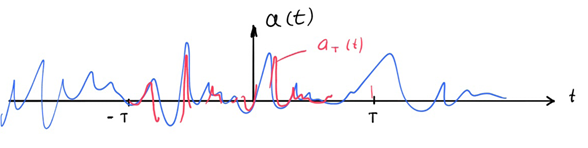
\includegraphics[scale=1]{Imagenes/Truncada.png}
	\label{fig:Truncada}
	%		\captionsetup{justification=raggedright,font={scriptsize,bf,it}}
	%		\caption*{fuente: http://superkuh.com/rtlsdr.html}
\end{figure}

Como puede observarse, entre más grande sea T, más alta es la exactitud en el cálculo del promedio de una señal.

\subsection{La Media de una Señal x(t)}

La Media De una señal x(t): La media De una señal x(t): 
 
 \begin{equation} \label{equ_veinticinco}
	 X_{m} = <x(t)> 
 \end{equation} 

\subsection{La Media Cuadrática de una Señal x(t)}
La Media Cuadrática De Una señal x(t): La media cuadrática de Una señal x(t):

 	\begin{equation} \label{equ_veintiseis}
		 X_{c} = <x^{2}(t)> 
	\end{equation}

\subsection{El Valor RMS}

El Valor RMS (del inglés Root Mean Square que se traduce como Raiz del Valor Medio Cuadrático)  de Una señal x(t): El Valor RMS de una Señal x(t):

	 \begin{equation} \label{equ_veintisiete}
	 	X_{RMS} = \sqrt{<x^{2}(t)>} 
	\end{equation}

\subsection{La Potencia Promedio de una Señal x(t)}

La Potencia Promedio Normalizada De Una señal

\begin{equation} \label{equ_veintiocho}
	 P = X_{RMS}^{2} = <x^{2}(t)> 
\end{equation} 


\textbf{Nota: el término “normalizada” es porque se considera $R=1 \Omega$}

\subsection{La Función de Autocorrelación}

La Función de Autocorrelación de x(t): La Función de Autocorrelación de x(t):

 \begin{equation} \label{equ_veintinueve}
	 R_{X}(\tau) = <x(t) x(t + \tau)> = \lim_{T \to \infty} \dfrac{1}{2T} \int_{-T}^{T} x(t) x(t + \tau) d\tau 
\end{equation}
Es importante notar que:
\begin{itemize}
    \item la Función de Autorrelación evaluada en $\tau =0$, es igual a la media cuadrática de la señal
    \item Por lo anterior, si la media de la señal es cero, entonces la Función de Autorrelación evaluada en $\tau =0$, es igual a la Potencia Promedio de la señal.
\end{itemize}    
\subsection{Otros promedios de tiempo}
La Varianza
\begin{equation} \label{equ_veintiocho}
	 {\sigma_x}^2= <[x(t)-X_m]^2>
\end{equation} 
La Desviación Estándar
\begin{equation} \label{equ_veintiocho}
	 \sigma_x= \sqrt{<[x(t)-X_m]^2>}
\end{equation} 

\subsection{Promedios de tiempo en señales complejas}
En el caso de las señales complejas es especial, ya que una señal es una especie de matrimonio entre una señal real y una imaginaria, de modo que es una pareja inseparable de señales. En este caso, es importante tener en cuenta lo siguiente:
\begin{itemize}
    \item una señal compleja, aunque es un apareamiento entre dos señales, puede ser vista como una sola cosa si se representa como un vector en el plano complejo, el cual puede variar diversos parámetros como su velocidad, su magnitud, su fase.
    \item hablar del promedio de tiempo en una señal compleja es hablar del comportamiento promedio del vector.\\
    \item El promedio de tiempo se puede definir como el valor complejo, donde la parte real y la imaginaria resultan de sacar el promedio de tiempo de la parte real de la señal y de la parte imaginaria respectivamente. Lo cual, se traduce en el punto del plano complejo donde hay mayor probabilidad de encontrar al vector.
    \item En el caso de la media cuadrática es un tanto diferente; en vez de la media cuadrática, lo que se usa es la magnitud cuadrática media del vector en el plano complejo. Pero igualmente resulta en un valor complejo, donde la parte real y la imaginaria resultan de sacar la media cuadrática de la parte real de la señal y de la parte imaginaria respectivamente. Lo cual, se traduce en la longitud al cuadrado que tiene mayor probabilidad de encontrarse el vector.
    \item La magnitud media, se deduce de lo dicho anteriormente, ya que es la raiz cuadrada del magnitud cuadrática media.
    \item En este caso, la Potencia Promedio de una señal es claramente el cuadrado de la magnitud media.
\end{itemize}

De acuerdo a las consideraciones anteriores, la media de una señal compleja aleatoria es un valor complejo y le corresponde esta fórmula:

 	\begin{equation} \label{equ_veintiseis}
		 X_{m} = <x_{r}(t)>+j<x_{i}(t)> 
	\end{equation}
Donde $x_{r}(t)$ y $x_{i}(t)$ corresponden a la parte real y a la imaginaria respectivamente de la señal analizada 

La Magnitud media cuadrática de una señal compleja aleatoria es un valor real y le corresponde la siguiente fórmula:

 	\begin{equation} \label{equ_veintiseis}
		 |X_{c}| = <|x(t)|^{2}> 
	\end{equation}

También es válido decir que:
 	\begin{equation} \label{equ_veintiseis}
		 |X_{c}| = X_{rc}+X_{ic} 
	\end{equation}
Donde $X_{rc}$ y $X_{ic}$ son la media cuadrática de la parte real y de la parte imaginaria respectivamente de la señal analizada $x(t)$
A la Función de Autocorrelación le corresponde la fórmula:

 \begin{equation} \label{equ_veintinueve}
	 R_{X}(\tau) = <|x(t) x(t + \tau)|> = \lim_{T \to \infty} \dfrac{1}{2T} \int_{-T}^{T} |x(t) x(t + \tau)| d\tau 
\end{equation}

Potencia promedio normalizada es:
 	\begin{equation} \label{equ_veintiseis}
		 P=X_{c} 
	\end{equation}
De igual manera, se puede deducir que el Valor RMS para las señales complejas es:

	 \begin{equation} \label{equ_veintisiete}
	 	X_{RMS} = \srqt{|X_{c}|} = \sqrt{<|x(t)^{2}>}=\srqt{<|x(t)|>} 
	\end{equation}

	 \begin{equation} \label{equ_veintiocho}
	 	X_{RMS} = \sqrt{|X_c|} + \sqrt{|x(t)|^{2}>} + <|x(t)|>
	\end{equation}

\subsection{La Densidad Espectral de Potencia}



La PSD como un promedio de tiempo: Ya se ha dicho que la PSD es la distribución de la potencia promedio, de la señal analizada en el espectro de frecuencias. La PSD de una señal $x(t)$ se representa como $S_{X}(f)$. \\

Debido a la anterior afirmación se obtiene que:\\ 

\begin{equation} \label{equ_treinta}
	P =  \int_{-\infty}^{\infty} S_{X}(f) df 
\end{equation}

Aprovechando la relación de Parseval podemos encontrar dos maneras alternativas para hallar la Potencia Promedio de una señal $x(t)$:

\begin{equation} \label{equ_treintauno}
	 P = \lim_{T \to \infty} \dfrac{1}{2T} \int_{-\infty}^{\infty} |X_{T}(t)|^{2}dt  ;  P = \lim_{T \to \infty} \dfrac{1}{2T} \int_{-\infty}^{\infty} |X(f , T)|^{2}df 
\end{equation}

Donde $X(f,T)$ es la TF de $x_{T}(t)$ , luego: \\

\begin{equation} \label{equ_treintados}
X(f,T) = \int_{-\infty}^{\infty} x_{T}(t)e^{-j2\pi ft} dt = \int_{-T}^{T} x/(t)e^{-j2\pi ft} dt 
\end{equation}

Se deduce entonces que:

\begin{equation} \label{equ_treintatres}
	 S_{X}(f) = \lim_{T \to \infty} \frac{1}{2T} |X(f, T)|^{2} 
\end{equation}

Como es bien sabido, las dimensiones de la TF son en V/Hz, de modo que las de la TF en magnitud al cuadrado son en $Watts/Hz^{2}$. Por lo tanto, las de la PSD son de $watts/Hz$. Nota: se están considerando valores normalizados para $R = 1\Omega$ . Esto es útil cuando solo se desea conocer la forma del espectro, sin embargo, para mediciones más precisas de espectro, por ejemplo cuando se desea conocer el espectro que captura la antena de un USRP, hay que tener en cuenta que R es la impedancia del medio donde se mide la señal. El problema es que la impedancia de una antena es diferente para cada frecuencia.\\
\subsection{Relación de la Densidad Espectral de Potencia con la Función de Autocorrelación}
Existe una importante relación entre PSD y autocorrelación de una señal aleatoria la cual se expresa de la siguiente manera:
$S_{X}(f)$ es también la TF de $R_{X}(\tau)$ entonces, $S_{X}(f)=\int_{-\infty}^{\infty} R_{X}(\tau)e^{-j2\pi f\tau} d\tau$. Consecuentemente la potencia promedio se puede hallar también como $P=R_{X}(0)$.\\

\subsection{Periodograma}

Es la Gráfica que corresponde a la expresión $\dfrac{1}{2T}|X(f,T)|^{2}$ cuando se obtiene con elementos de cómputo. \\

En este caso resulta más útil la formulación

\begin{equation} \label{equ_treintacuatro}
  S_{x}(f) = \lim_{T \to \infty} \dfrac{1}{2T} |X(f,T)|^{2} = <|X(f)|^{2}> 
\end{equation}

La idea es caer en cuenta que esta fórmula expresa un promedio. En simulink o en GNU Radio se puede ir mostrando cómo se va calculando ese promedio a medida que pasa el tiempo. De modo que no es necesario esperar a que transcurra todo el tiempo T para visualizar la PSD. \\

%\vspace{200px}
\begin{figure}[h!]
	\captionsetup{justification = raggedright, singlelinecheck = false}
	\caption{Ejemplo de periodograma} 
	\centering
	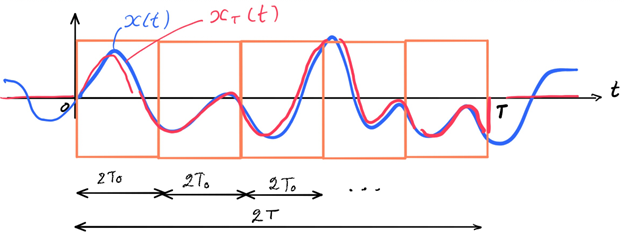
\includegraphics[scale=0.8]{Imagenes/Periodograma.png}
	\label{fig:Ejemplo-periodo}
	%		\captionsetup{justification=raggedright,font={scriptsize,bf,it}}
	%		\caption*{fuente: http://superkuh.com/rtlsdr.html}
\end{figure}

La idea es dividir el tiempo de medición T en pequeñas ventanas de duración $T_{0}$. Entonces la señal truncada $X_{T}(t)$ se divide en señales sub truncadas de más corta duración $ x_{T,1}(t), x_{T,2}(t), .... , x_{T,N}(t) $ De esta manera, es posible hallar paso a paso $ |X_{1}(f,T)|^{2}, |X_{2}(f,T)|^{2}, .... , |X_{N}(f,T)|^{2} $ consecuentemente se puede hallar la PSD aproximada de esas señales sub truncadas $ S _{X,1}(f,T), S _{X,2}(f,T).... S _{X,N}(f,T)$. Si en cada uno de esos pasos se va realizando un ajuste, será posible obtener y graficar la PSD para el tiempo $ 2T_{0}, 4T_{0}, 6T_{0}, ..... , 2T$. . Como resultado veremos como la PSD va tomando poco a poco una forma cada vez más definida. Lo que se logra es que el usuario no tenga que esperar mucho tiempo para ver la PSD, sino que en tiempo real pueda ver como la PSD va tomando una forma cada vez más definitiva. Para el ajuste mencionado solo hay que tener en cuenta que la PSD es un promedio, pero eso se explicará más abajo en una implementación que usa la FFT como bloque de cálculo de la Transformada de Fourier Truncada. \\

Uso del bloque FFT de GNU Radio para obtener la PSD. La idea es usar el bloque de GNU Radio que implementa el algoritmo FFT en magnitud al cuadrado, que simbolizaremos así:
$|FFT|^{2}$. En la página web del libro, se tiene una demostración donde se usa Simulink de Matlab para demostrar lo anterior, este es el enlace:

\begin{center}
\url{https://sites.google.com/saber.uis.edu.co/comdig/m/Analizador}
\end{center}

\subsection{Señal Binaria Bipolar Aleatoria}
Uno de los primeros pasos en el estudio de las comunicaciones consiste en conocer y analizar ciertas señales que son claves. Una de ellas son las señales binarias bipolares aleatorias.\\ 
Obtenemos primero La función de autocorrelación. Tomaremos como ejemplo la señal $x(t)$. de la Figura \ref{fig:Ejemplo} donde $T_b$ es el ancho de cada pulso que en términos de señales digitales, puede ser equivalente a la duración de un bit.

\begin{figure}[h!]
	\captionsetup{justification = raggedright, singlelinecheck = false}
	\caption{Ejemplo de una señal binaria aleatoria bipolar $x(t)$ } 
	\centering
	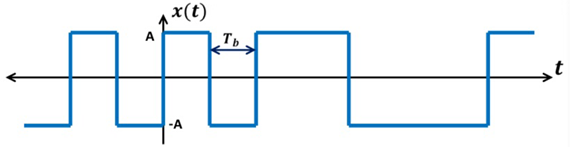
\includegraphics[scale=0.9]{Imagenes/Ejemplo.png}
	\label{fig:Ejemplo}
	%		\captionsetup{justification=raggedright,font={scriptsize,bf,it}}
	%		\caption*{fuente: http://superkuh.com/rtlsdr.html}
\end{figure}

Recordemos que $ R_{X}(\tau) = <x(t)x(t + \tau)> = \lim_{T \to \infty} \dfrac{1}{2T} \int_{-T}^{T} x(t) x(t + \tau ) d\tau $. En la Figura \ref{fig:Ejemplo1} set tiene la forma de la señal $x(t+\tau)$ cuando $\tau<T_b$\\

\begin{figure}[h!]
	\captionsetup{justification = raggedright, singlelinecheck = false}
	\caption{El desplazamiento de la señal binaria aleatoria bipolar que resulta en la señal $\tau < T_b $} 
	\centering
	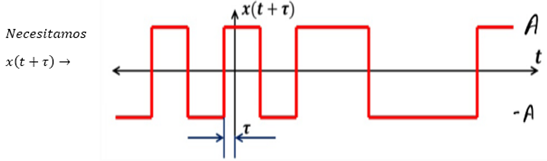
\includegraphics[scale=1]{Imagenes/Ejemplo1.png}
	\label{fig:Ejemplo1}
	%		\captionsetup{justification=raggedright,font={scriptsize,bf,it}}
	%		\caption*{fuente: http://superkuh.com/rtlsdr.html}
\end{figure}
Vamos a revisar los siguientes casos:
\begin{itemize}
    \item Caso en que $\tau = 0$:\\
Tenemos que $<x(t) x(t + \tau )> =<x^{2}(t)>=<A^{2}>=A^{2}$
    \item Caso en que $0<\tau<T_b$:\\
En este caso, la operación $x(t)x(t+\tau)$ tiene la forma que se presenta en la Figura \ref{fig:Ejemplo2}.
\begin{figure}[h!]
	\captionsetup{justification = raggedright, singlelinecheck = false}
	\caption{Multiplicación de la señal $x(t)$ con su versión desplazada $x(t+\tau)$ cuando $0<\tau < T_b$}
	\centering
	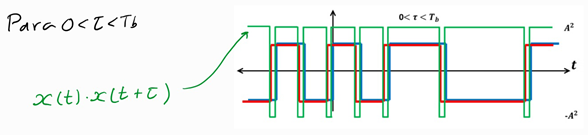
\includegraphics[scale=1]{Imagenes/Ejemplo2.png}
	\label{fig:Ejemplo2}
	%		\captionsetup{justification=raggedright,font={scriptsize,bf,it}}
	%		\caption*{fuente: http://superkuh.com/rtlsdr.html}
\end{figure}
    \item Caso en que  $ \tau = T_{b}$:
Tenemos que la multiplicación $x(t)x(t+\tau)$ resulta siendo una nueva señal binaria aleatoria bipolar como se muestra en la Figura \ref{fig:Ejemplo3}.
\begin{figure}[h!]
	\captionsetup{justification = raggedright, singlelinecheck = false}
	\caption{Multiplicación de la señal $x(t)$ con su versión desplazada $x(t+\tau)$ cuando $0<\tau = T_b$}
	\centering
	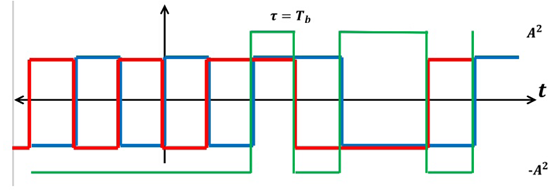
\includegraphics[scale=0.9]{Imagenes/Ejemplo3.png}
	\label{fig:Ejemplo3}
	%		\captionsetup{justification=raggedright,font={scriptsize,bf,it}}
	%		\caption*{fuente: http://superkuh.com/rtlsdr.html}
\end{figure}
\end{itemize}

Vemos que para $ \tau = 0, x(t)x(t + \tau ) = A^{2}$ y su promedio de tiempo es $<x(t)x(t+\tau ) > A^{2}$ que es la misma potencia promedio. Cuando $0 < \tau < T_{b}$ el promedio de tiempo de $x(t)x(t+\tau)$ cae linealmente.
Cuando $ \tau = T_{b}$  ocurre que $x(t)x(t + \tau)$ se convierte en una nueva señal binaria bipolar aleatoria, cuyo promedio de tiempo es cero. Algo similar ocurre cuando $\tau > T_{b}$.
Ahora, cuando $\tau < 0$ ocurre lo mismo que cuando $\tau > 0$.


Es importante tener en cuenta que la Función de Autocorrelación evaluada en cero es la misma potencia promedio $P=R_{X}(0)$, solo que para el caso dado, $P=R_{X}(0)=A^2$. De modo que la función de autocorrelación tiene la forma de la Figura \ref{fig:Triangulo}.

%\vspace{200px}
\begin{figure}[h!]
	\captionsetup{justification = raggedright, singlelinecheck = false}
	\caption{La Función de Autocorrelación de una señal binaria aleatoria bipolar} 
	\centering
	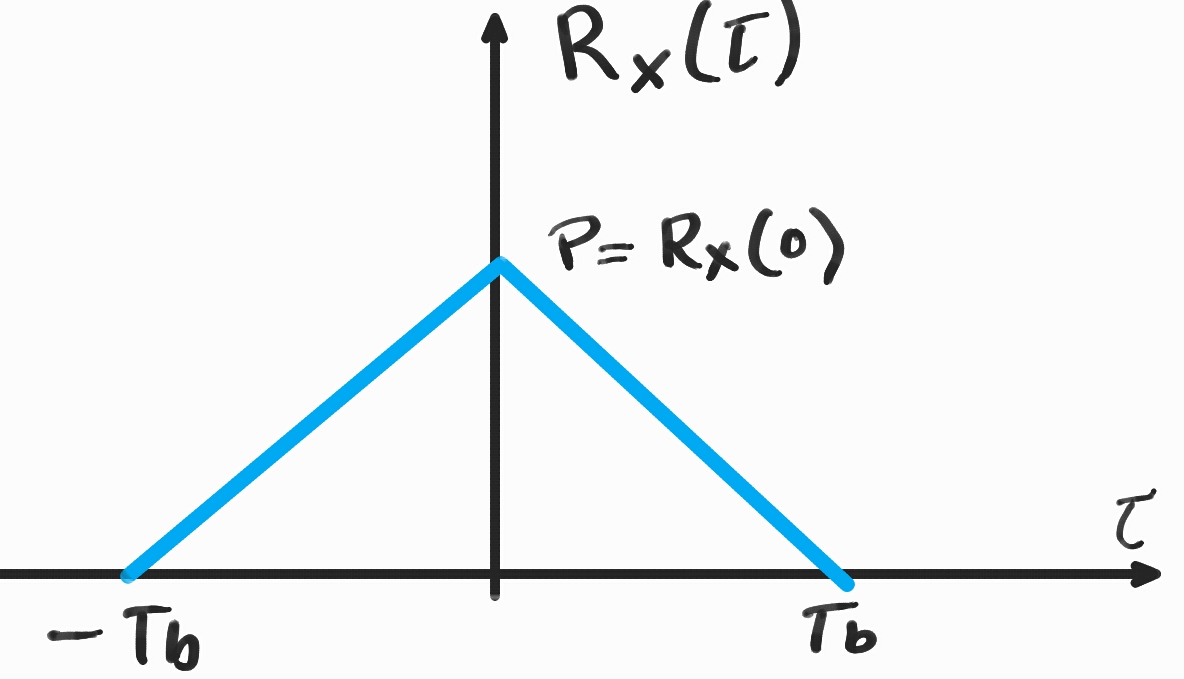
\includegraphics[scale=0.3]{Imagenes/Triangulo.png}
	\label{fig:Triangulo}
	%		\captionsetup{justification=raggedright,font={scriptsize,bf,it}}
	%		\caption*{fuente: http://superkuh.com/rtlsdr.html}
\end{figure}

Recordemos que la PSD es la TF de la Función de Autocorrelación. De manera que podemos usar la Función de Autocorrelación obtenida para buscar la forma de la PSD. Para ello, expresamoos la Función de autocorrelación como una Convolución así:

\begin{equation} \label{equ_treintacinco}
	 R_{x}(\tau) =\frac{1}{T_{b}} R_{X1}(\tau) * R_{X1}(\tau) 
\end{equation}

Donde $R_{X1}(\tau)$ tiene una forma rectangular como se muestra en la siguiente figura \ref{fig:Cuadrado}.



\begin{figure}[h!]
	\captionsetup{justification = raggedright, singlelinecheck = false}
	\caption{ Forma de $R_{X1}(\tau)$} 
	\centering
	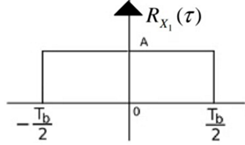
\includegraphics[scale=1]{Imagenes/Cuadrado.png}
	\label{fig:Cuadrado}
	%		\captionsetup{justification=raggedright,font={scriptsize,bf,it}}
	%		\caption*{fuente: http://superkuh.com/rtlsdr.html}
\end{figure}

De esta manera podemos usar la TF de una señal de forma rectangular, la cual es bien conocida y que se muestra en la Figura \ref{fig:Cuadrado-dos}.

\begin{figure}[h!]
	\captionsetup{justification = raggedright, singlelinecheck = false}
	\caption{$R_{X_1}(\tau)$ y su Transformada de Fourier} 
	\centering
	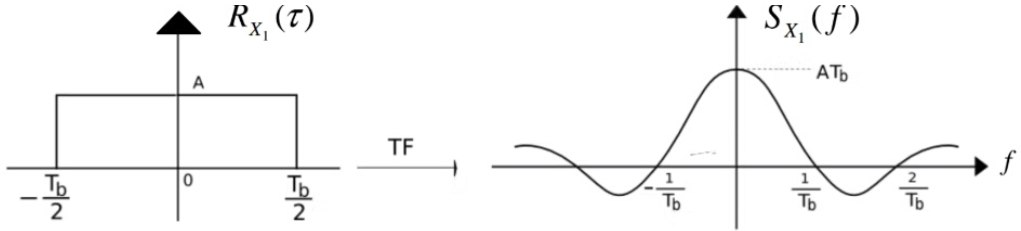
\includegraphics[scale=0.6]{Imagenes/Cuadrado-dos.png}
	\label{fig:Cuadrado-dos}
	\captionsetup{justification=raggedright,font={scriptsize,bf,it}}
\end{figure}

Nótese que $S_{X_1}(f)$ estaría dado en V/Hz tal como se conoce la TF de una señal cuadrada. \\
También aprovechamos el Teorema de la Convolución, también conocido como Teorema de Wiener Khitchine que dice que si se tiene:

\begin{equation} \label{equ_treintaseis}
	x_{1}(t) = \overset{TF}{\rightarrow} X_{1}(f) 
\end{equation}
y
\begin{equation} \label{equ_treintasietex}
	x_{2}(t) = \overset{TF}{\rightarrow} X_{2}(f)
\end{equation}

Entonces
\begin{equation} \label{equ_treintasiete}
	 x_{1}(t) * x_{2}(t) \overset{TF}{\rightarrow} X_{1}(f) X_{2}(f)
\end{equation}

Luego,

\begin{equation} \label{equ_treintaocho}
\frac{1}{T_b}R_{X_1}(\tau )*R_{X_1}(\tau )\overset{TF}{\rightarrow}\frac{1}{T_b}S^{2}_{X_{1}}(f)
\end{equation}

\begin{figure}[h!]
	\captionsetup{justification = raggedright, singlelinecheck = false}
	\caption{ PSD de la forma Forma de $R_{X1}(\tau)$} 
	\centering
	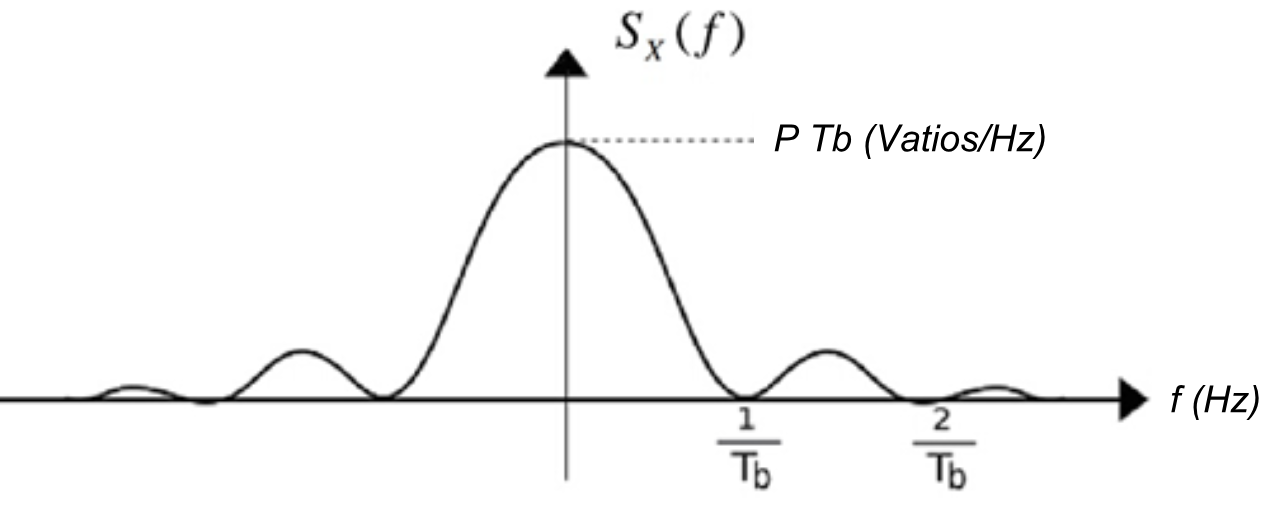
\includegraphics[scale=0.4]{Imagenes/PSD.png}
	\label{fig:PSD}
	%		\captionsetup{justification=raggedright,font={scriptsize,bf,it}}
	%		\caption*{fuente: http://superkuh.com/rtlsdr.html}
\end{figure}
De esta manera se obtiene que la forma de la PSD de una señal binaria aleatoria bipolar corresponde a la función sinc cuadrática:
\begin{equation} \label{equ_treintasietess}
	 S_X(f)=P T_b sinc^2(f/R_b)
\end{equation}
donde $R_b=1/Tb$ es la rata de bits. La gráfica de la PSD de una Función Binaria Aleatoria Bipolar se presenta en la Figura \ref{fig:PSD}.

\subsection{El ruido blanco}

El ruido blanco (WN, del inglés White Noise) siempre está presente en cualquier medio de propagación, pero no deja de ser una abstracción matemática, debido a ciertos supuestos como: 

\begin{itemize}
	
	\item  Tienen un ancho de banda infinito. De allí viene el término “blanco”, pues se supone que el color blanco resulta de combinar homogéneamente todos los colores (las frecuencias).
	\item  La Densidad Espectral de Potencia es constante e igual a $N_0/2$, donde 

\begin{equation} \label{equ_treintanueve}
		 N_0 = kT_e
\end{equation}

Donde $k$ es la constante de Boltzmann y $T_e$ es la temperatura equivalente del ruido en el receptor. La idea de la temperatura equivalente proviene de experimentos realizados con sistemas electrónicos, donde se ha observado a que a medida que aumenta la temperatura en estos sistemas, aumenta el ruido. En gran manera puede estar dado por las características del receptor, pero también por cuestiones naturales en el espectro.

	\item  La función de autocorrelación es una función delta centrada en cero, como se muestra en la Figura \ref{fig:Funcion}, lo cual significa que dos muestras del ruido, por muy cercanas que sean no están correlacionadas, de modo que una muestra aparece correlacionada solo con sí misma. En este sentido, el ruido blando es lo último en aleatoriedad.
	
%	\setcounter{figure}{47}
	\begin{figure}[h!]
		\captionsetup{justification = raggedright, singlelinecheck = false}
		\caption {PSD del ruido blanco y su Función de autocorrelación} 
		\centering
		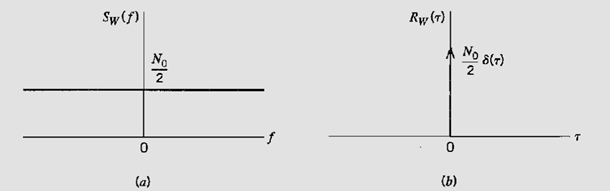
\includegraphics[scale=0.9]{Imagenes/Funcion.png}
		\label{fig:Funcion}
				\captionsetup{justification=raggedright,font={scriptsize,bf,it}}
				\caption*{fuente: Tomado del libro de Haykin}
	\end{figure}
	\item  Conocer el desempeño de un sistema de comunicaciones frente al ruido blanco que puede presentarse en el canal, no deja de ser una idealización, pero sirve de referencia para caracterizar el sistema y los métodos usados en el procesamiento de la información.  
\end{itemize}


\subsection{La voz humana} en la telefonía

El sonido es uno de los principales tipos de mensajes que se emiten por los medios de comunicación y se usa intensamente en ejemplos y prácticas de este libro, sobre todo los sonidos que el ser humano emite para comunicar. La voz es toda una ciencia, sinembargo, para los propósitos del presente libro los siguientes apuntes son los de mayor relevancia:
\begin{itemize}
    \item el sonido son ondas mecánicas longituinales, se desplazan de un lugar a otro mediante perturbaciones de un medio elástico (sólido, líquido, gaseoso).
    \item Las ondas sonoras se reducen a los límites de frecuencia que pueden estimular el oido humano para ser percibidas en el cerebro.
    \item los límites de frecuencia de las ondas sonoras se extienden de aproximadamente 20 Hz a cerca de 20 kHz y se llaman límites de audición.
    \item La voz está constituida por un conjunto de sonidos generados por el aparato fonador, de manera que tiene un menor rango de frecuencias que el sonido
    \item En aplicaciones reales de comunicaciones, una señal de voz es una señal aleatoria, desde este punto de vista sus características son de tipo aleatorio, pero además depende de cada persona.
    \item De acuerdo a los estudios tenidos en cuenta por la UIT, la mayor energía de la voz se encuentra concentrada por debajo de los 4 kHz. De modo que la UIT ha establecido que para los propósitos de la telefonía, la señal de la voz puede estar limitada a 4 kHz. Es por eso que, al implementarse las tecnologías digitales en la frecuencia fija, se estableció que la frecuencia de muestreo es de $Samp rate   audio=8$  kHz. También se estableció que los niveles de cuantificación son 256, lo cual equivale a 8 bits por muestra ya que $NbpS=256=2^8 $ 
    \item De lo anterior se deduce que la rata de bits en la telefonía es de $Rb=Samp rate audio x Nbps=64$ kbps.
\end{itemize}

\section{Variable aleatoria.}
\subsection{Introducción}
Arriesgarse a estudiar y sobre todo a practicar con señales aleatorias  significa arriesgarse a contactar con el mundo real. Esto es así, pues en el mundo real las señales son usualmente aleatorias. Pero surge una pregunta: ¿No basta con haber estudiado el tema de promedios de tiempo para realizar aplicaciones basadas Radio Definida por Software (SDR)? La respuesta es que sí. Sin embargo, estudiar el tema de Variable Aleatoria significa una especie de reconciliación con los matemáticos que trabajan en función de aplicaciones más amplias, que muchas veces no tienen que ver con señales, pero que pueden ser adaptadas a las señales y a los sistemas.\\ 
A manera de ejemplo, imaginemos que contamos con una señal de ruido discreta $x[n]$ de $N$ muestras y que hemos convocado a diferentes expertos a hablar sobre ella y a realizar demostraciones. Nosotros, realizaríamos quizá una simulación con gnuradio para mostrar cómo esta señal $x[n]$ esa compuesta de las muestras $x[1], x[2], ..., x[N]$ que tienen un comportamiento en tiempo y en frecuencia. También podríamos mostrar promedios de tiempo de esa señal, como la media, la varianza, etc. 
El siguiente experto podría ser un matemático o un ingeniero de sistemas que es muy hábil usando las herramientas que traen muchos lenguajes de programación para realizar operaciones vectoriales y matriciales que agilizan de manera severa el desarrollo de código. Entonces prefiere ver esa señal como un vector $\Vec{X}=[x_1, x_2, ...., x_{N}]$ al cual podrá manejar mediante operaciones vectoriales o matriciales. 
Supongamos que el experto es ahora un profesor de estadística acostumbrado a estudiar el comportamiento de ciertas variables como el precio del dolar, la frecuencia de las lluvias, etc. Este profesor prefería ver la  señal como un dataset o conjunto de los datos de las amplitudes que puede tomar la señal para obtener diversos parámetros y conceptos estadísticos como: la media, la varianza, pero también la función de densidad de probabilidad, la función de distribución acumulativa, la autocorrelación, entre otros. En este caso, la variable aleatoria y los promedios de tiempo son una misma cosa. Pero una variable aleatoria es un concepto más general pues abarca muchos otros casos, donde los datos que toma la variable no dependen necesariamente del tiempo. Por ejemplo, supongamos que la variable aleatoria $Z$ está compuesta de los N valores que resultan al lanzar un dado N veces. Esos N resultados no dependen del tiempo ni tienen nada que ver con las amplitudes de las señales.\\ 
En conclusión, lo que se gana al usar el concepto de Variable Aleatoria es la posibilidad de aprovechar en las comunicaciones los avances que existen en la estadística. La podemos usar como una alternativa a los promedios de tiempo. Para ello basta con suponer que cada muestra de la señal es el resultado de un ensayo. Pero el concepto de variable aleatoria se puede usar en un sentido más amplio donde los parámetros a analizar no son necesariamente valores de amplitud que cambian en el tiempo. En todo caso, el estudio del tema de Variable Aleatoria es imprescindible para llegar a estudiar el tema de Procesos Estocásticos que es una rama más genérica aún para estudiar las señales aleatorias en un sentido más amplio, por ejemplo, cuando nos interesa conocer el promedio de las voces de todos mis estudiantes, lo cual resulta en una nueva señal de tiempo que es el promedio de todas\\

Para aclarar aún más el concepto de variable aleatoria, supongamos que usted ha sido contratado para  para caracterizar la estatura de los estudiantes de su universidad. Entonces usted decide usar los siguientes parámetros: la estatura promedio, la desviación estándar, entre otros. Luego, usted decide realizar un experimento: medir de manera aleatoria a cada estudiante que entra ese día a la universidad. También querrá medir de manera aleatoria otras cosas que pueden guardar relación obvia o no tan obvia con la estatura como: la edad o el número de calzado, el sexo. Entonces crea una tabla con una columna para cada una de las mediciones, donde X representa la estatura, Y la edad y Z el calzado. X, Y, Z - son variables aleatorias. \\
En conclusión, el concepto de variable aleatoria es útil en las comunicaciones, cuando se desea interpretar las caracterísiticas de las señales o de los sistemas como datos para aplicarle conceptos estadísticos para llegar a algún tipo de conclusión válida.


\begin{table}[h!]
	\captionsetup{justification = raggedright,singlelinecheck = false}
	\caption{\label{tabla:tabla1} Alguna descripción}
		\centering
		\scalebox{0.75}{
\begin{tabular}{|l|l|l|l|}
\hline
Ensayo & X   & Y   & Z   \\ \hline
1      & $x_{1} = 1.80$   & $y_{1} = 18$   &  $z_{1} = 40$   \\ \hline
2      & $x_{2} = 1.70$   & $y_{2} = 20$   &  $z_{2} = 39$   \\ \hline
3      & $x_{3} = 1.73$   & $y_{3} = 17$   &  $z_{3} = 43$  \\ \hline
...    & ... & ... & ... \\ \hline
\end{tabular}}
\end{table}

También puede usar la siguiente notación: \\
$X= {x_{1}, x, x,...}$ \\

\subsection{Principales conceptos de variable aleatoria}

Los siguientes son los principales términos usados: \\

\textbf{Ensayo (realization):} Cada prueba que usted realiza. \\

\textbf{ Punto Muestra o Punto Muestral (sample point):} El resultado de cada ensayo, en este caso xi es el punto muestral del ensayo i de la variable aleatoria X. \\

\textbf{ Espacio muestral (Sample Space):} Es el conjunto de todos los puntos muestra posible para variable aleatoria. \\

\textbf{ La Esperanza (average or expected value):} Es la manera de referirse al promedio de puntos muestra y se representa como E[variable aleatoria] así: \\


\begin{equation} \label{capuno_variable}	
E[X]= \dfrac{x_{1} + x_{2} + ... + x_{N} }{N} ; E[X^{2}]= \dfrac{x_{1}^{2} + x_{2}^{2} + ... + x_{N}^{2} }{N}
\end{equation}

\begin{equation} \label{capuno_variabledos}	
E[({X-A})^{2}]=  \dfrac{{(x_{1}-A)}^{2} + {(x_{2}-A)}^{2} + ... + {(x_{N}-A)}^{2} }{N}
\end{equation}

$N$ Es el número de puntos muestra tenidos en cuenta. \\
Pero hay casos en que no se conocen los puntos muestra sino otros parámetros que se han obtenido a partir de ellos y que también definen la variable aleatoria como la Función de Densidad de Probabilidad $f_{X}(x)$. Por eso hay otras formas para obtener la Esperanza como $E[X]=-\int_{\infty}^{\infty}xf_{X}(x)dx$. \\

\textbf{ La media de una variable aleatoria} $X: \mu X=E[X]$ \\
\textbf{ La media cuadrática de una variable aleatoria} X: Corresponde a $E[X^{2}]$ \\
\textbf{ La varianza de una variable aleatoria} $X: var[X]=E[{(X- \mu X)}^{2}]= {\sigma}_{X}^{2}$ \\
\textbf{ La Desviación estándar de} $ X :$ es ${\sigma}_{X}$\\
\textbf{ La correlación entre las variables} $ X,Y: R_{XY}=E[XY]$\\

\subsection{La Función de densidad de probabilidad}
La Función de Densidad de Probabilidad (FDP) describe la probabilidad que puede cada valor que puede tomar una variable aleatoria. También permite conocer la probabilidad de que una variable aleatoria caiga dentro de un rango de posibles valores. Para los propósitos de este resumen, resulta suficiente comprender lo que representa la curva de la FDP en un ejemplo como el que se presenta en la en la figura \ref{fig:fdp}. 


\begin{figure}[h!]
	\captionsetup{justification = raggedright, singlelinecheck = false}
	\caption{Ejemplo de la Función de Densidad de probabilidad} 
	\centering
	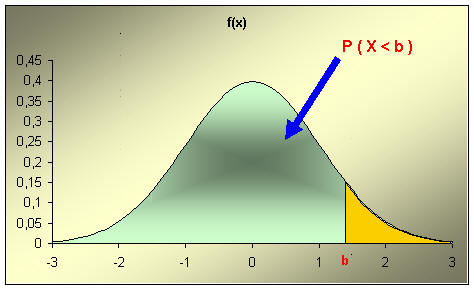
\includegraphics[scale=0.5]{Imagenes/probcon3.jpg}
	\label{fig:fdp}
% Lo siguiene es para indicar la fuente de la cual fue tomada la figura
  \captionsetup{justification=raggedright,font={scriptsize,bf,it}}
\end{figure}

Para el ejemplo que representa esa figura, podemos observar que la probabilidad de que la variable aleatoria $X$ tome el valor 1 es aproximadamente 0,15, que si se expresa en porcentaje, equivale al 15\%. El área bajo la curva de la FDP es siempre igual a 1. La probabilidad de que la variable aleatoria tome un valor menor que b, es decir $P(X<b)$ es igual al área bajo la curva desde $-\infty$ hasta b y para el ejemplo dado en la figura \ref{fig:fdp} se encuentra sombreada en color azul. De manera similar, buscando siempre el área bajo la curva entre intervalos diversos es posible encontrar la probabilidad de que $X$ tome cualquier otro rango de valores.\\

Un aspecto muy importante a tener siempre en cuenta es que al FDP caracteriza completamente a una variable aleatoria. Es decir, si se conoce la FDP de una variable aleatoria, ya se tiene toda la información sobre esa variable.


En gnuradio es común aproximarse a la FDP mediante lo que se conoce como un histograma, mientras que el uso de una forma continua de la FDP es más común en los análisis teóricos. En los histogramas usualmente se considera que la variable aleatoria puede tomar un número finito de valores discretos, como se muestra en el ejemplo de la figura \ref{fig:histo}. 

\begin{figure}[h!]
	\captionsetup{justification = raggedright, singlelinecheck = false}
	\caption{Ejemplo de un histograma} 
	\centering
	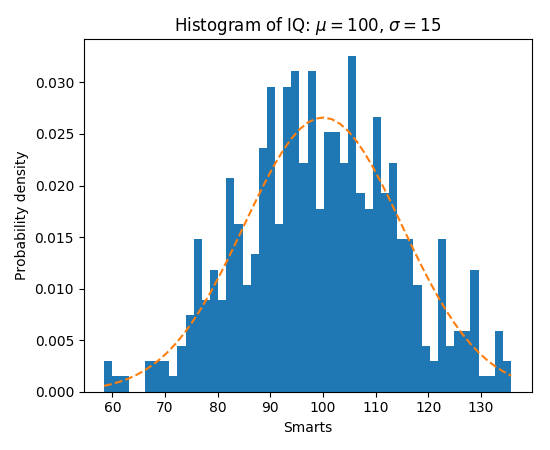
\includegraphics[scale=0.5]{Imagenes/histogram_demo_features.png}
	\label{fig:histo}
% Lo siguiene es para indicar la fuente de la cual fue tomada la figura
  \captionsetup{justification=raggedright,font={scriptsize,bf,it}}
  \caption*{fuente: Matplolib}
\end{figure}

\subsection{La Función de Distribución Acumulativa}
La Función de Distribución Acumulativa (FDA) es otra manera de caracterizar completamente una variable aleatoria, pero no es nada nuevo con respecto a la FDA, sino más bien una deducción de ella, ya que la FDA se puede expresar como

\begin{equation} \label{equ:fda}
	 F(x)=\int\limits_{-\infty}^{x}  f(u)du,				
\end{equation}
donde $f(u)$ es la FDP de una variable aleatoria $U$.

\section{Procesos Estocásticos}

Los procesos estocásticos representan un mayor nivel de generalización de las variables aleatorias para poner la teoría de las probabilidades al servicio exclusivo de las señales aleatorias. En este sentido, es importante tener en cuenta las siguientes aclaraciones:
\begin{itemize}
    \item Una variable aleatoria toma valores que dependen de un ensayo. Por ejemplo, si el experimento consiste en medir la altura de los estudiantes, cada estudiante que medimos es un ensayo y la altura de medimos es una muestra de la variable aleatoria.
    \item Es posible hacer que una variable aleatoria tome como muestras los valores de amplitud que toma una señal en el tiempo, pero precisamente eso es un caso muy particular que hemos llamado Promedios de Tiempo. En los procesos estocásticos no se tiene esta posibilidad, ya que en un proceso estocástico una señal en el tiempo considerado como el resultado de un ensayo, por eso se habla de funciones muestra.
\end{itemize}

Para entenderlo mejor, supongamos que hemos sido contratados para caracterizar no la altura, sino la voz de los estudiantes de su universidad. Entonces, en lugar de medir la altura para llenar una lista de datos, lo que hacemos es grabar la voz de cada estudiante que pasa aleatoriamente y la guardamos. Entonces, ya no tenemos muestras discretas en forma de un valor por muestra, como era el caso para la altura, sino funciones funciones muestra, ya que cada muestra es una función de tiempo, como se muestra en la figura \ref{fig:Ensayo}.

	\begin{figure}[h!]
		\captionsetup{justification = raggedright, singlelinecheck = false}
		\caption{Ejemplo de Funciones muestra de un proceso estocástico $X(t)$} 
		\centering
		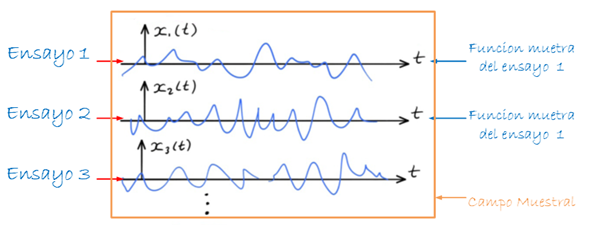
\includegraphics[scale=1]{Imagenes/Ensayo.png}
		\label{fig:Ensayo}
		%	\captionsetup{justification=raggedright,font={scriptsize,bf,it}}
		%	\caption*{fuente: \textcolor{
		%			Orange}{Tomada de Wikipedia}}
	\end{figure}
	
Por analogía con la variable aleatoria, un proceso estocástico se representa como:

\begin{equation} \label{capuno_variablecuatro}	
X(t) = {x_{1}(t), x_{2}(t), x_{3}(t),...} 
\end{equation}

$X(t)$ es lo que se conoce como un Proceso Estocástico. A diferencia de una variable aleatoria que se compone de puntos muestra, el proceso estocástico se compone de \textbf{funciones muestra (sample functions)}, en este caso esas funciones son: $x_{1}(t), x_{2}(t), x_{3}(t), ..., x_{N}(t)$., las cuales a su vez componen el \textbf{espacio muestral o campo muestral (sample space)}.\\
Todos los parámetros estudiandos que aplican a las variables aleatorias, puede generalizarse para los procesos estocásticos.

\textbf{La media de proceso} $X(t): \mu _{X(t)}=E[X(t)]$. Vemos que a diferencia de una Variable Aleatoria, donde la media es un número, en un Proceso Estocástico la media es una función del tiempo. \\

La media se obtiene de manera aproximada sumando N funciones muestra y dividiendo el resultado en N con lo cual se obtiene la señal promediada. $E[X(t)]= \dfrac{\sum_{n=1}^{N}x_{n}(t)}{N}$ \\

\textbf{La media cuadrática de $X(t)$} es  $E[X^{2}(t)]$.\\
\textbf{La Función de Autocorrelación de un Proceso Estacionario $X(t) $ } es $R_{x}( \tau )=E[X(t+ \tau )X(t)]$ \\
De manera similar se derivan todos los demás parámetros.

%%%%%%%%%%%%%%%%%%%%%%%%%%%%%%%%%%%%%%%%%
\section{Resumen de Señales y Sistemas Discretos}

\subsection{Teorema de Muestreo}
[Falta]

\subsection{La Representación en series de Fourier Discreta}

La Representación en Series de Fourier Discreta (RSFD) aplica lo mismo que se dijo para las señales continuas, pero con los siguientes aspectos y aclaraciones adicionales:

\begin{itemize}
	\item  La señal analizada $x_{N}[n]$ es discreta y periódica en N muestras.
	\item  La ecuación de análisis es

\begin{equation} \label{equ_cuarenta}
			 C_{k} = \dfrac{1}{N} \sum_{n=0}^{N-1}x_{N} [n]e^{-j2 \pi kn/N}		
\end{equation}	
\item  La ecuación de Síntesis es:
\begin{equation} \label{equ_cuarentas}
			 x_{N}[n] = \sum_{k=0}^{N-1}C_{k} e^{j2 \pi kn/N}		
\end{equation}
\end{itemize}
\subsection{La Transformada Discreta de Fourier}
La siguiente es la transformada de Fourier Discreta (DFT):\\
La Ecuación de Síntesis:
\begin{equation} \label{equ_DFT}
			 x[n] = \dfrac{1}{2\pi} \int_{2\pi}{X(e^{j\omega n})d\omega}		
\end{equation}	
Donde $\omega=2\pi f$.\\
La Ecuación de Análisis:
\begin{equation} \label{equ_DFTI}
			 X(e^{j\omega}) =  \sum_{n=-\infty}^{+\infty} {x[n]e^{-j\omega n}}		
\end{equation}
Sin embargo, las ecuaciones (\ref{equ_DFT}) y (\ref{equ_DFTI}) no dejan de ser una definición teórica ya que sirven para realizar análisis de tipo teórico, como se hace por ejemplo en el libro de Oppenheim \cite{Mejia2012} \textcolor{red}{[referenciar]}, pero requiere una redefinición para las aplicaciones del mundo real, sobre todo en el campo de las comunicaciones. El problema de las aplicaciones del mundo real en las comunicaciones consiste en lo siguiente:
\begin{itemize}
    \item La señal $x[n]$ proviene de una versión continua $x(t)$, con un ancho de banda definido, que es luego sometida a un muestreo.
    \item Al aplicar el proceso de muestreo se usa una frecuencia de muestreo $F_S$. Como resultado, la señal x[n] resulta acotada en el ancho de banda $BW=F_S/2$  
    \item En una aplicación pŕactica solo es posible procesar un número $N$ finito de muestras. Como resultado, la DFT del mundo real también tiene un número finito $N$ finito de muestras. Por lo tanto, la transformada de Fourier resulta siendo igualmente discreta como lo es la señal.
\end{itemize}
Por todo lo anterior, resulta necesario encontrar la expresión de la  DFT para aplicaciones del mundo real. En este sentido, vale la pena tener en cuenta los siguientes aspectos adicionales:
\begin{itemize}
    \item La DFT está directamente relacionada con la RSF.
    \item La principal diferencia de la DFT con respecto a la RSFD consiste en la manera en que se aplica. La  RSFD se aplica solo al periodo de la señal $x[n]$. La DFT debería aplicarse a toda la duración de esa señal, pero como eso no es posible solo se aplica a un número $N$ de muestras, luego, realmente lo que se obtiene es una aproximación de la DFT.
    \item Otra diferencia consiste en que la TF es, además de lo anterior, una versión escalada de la RSFD. El escalamiento corresponde a la duración de la señal, es decir al valor $N$
\end{itemize}
Por todo lo anterior la DFT, para propósitos prácticos, se puede decir de la siguiente manera:
\begin{itemize}
	\item  La señal analizada $x_[n]$ es discreta y tiene una duración de N muestras.
	\item  La ecuación de análisis es:
\begin{equation} \label{equ_DFT2}
			 X(k) = \lim_{N \to \infty} \sum_{n=0}^{N-1}x[n]e^{-j2 \pi kn/N}		
\end{equation}	
\item  La ecuación de Síntesis es:
\begin{equation} \label{equ_DFTi2}
			 x[n] = \lim_{N \to \infty} \frac{1}{N} \sum_{k=0}^{N-1}X(k) e^{j2 \pi kn/N}
\end{equation}
\end{itemize}
\subsection{La Transformada Rápida de Fourier}
Este capítulo no busca explicar de manera exhaustiva de donde sale ni cómo se calcula la Transformada Rápida de Fourier (FFT, del inglés Fast Fourier Transform), pues realmente hay buena literatura sobre este aspecto \textcolor{red}{[referenciar]}.\\ Nos detendremos en siguientes aspectos que nos interesan para los propósitos del libro:

\begin{itemize}
    \item La FFT es en realidad un algoritmo para ejecutar de manera computacionalmente más económica posible la siguiente operación:
    \begin{equation} \label{equ_fft}
			 X(k) = \sum_{n=0}^{N-1}x[n]W^{-kn},
    \end{equation} donde  $W=e^{-j2 \pi/N}$, $k=0,1,2, ... N-1$, $N = 2^m$, m es un número entero.
    \item Existe también la operación de síntesis conocida mejor como la Transformada Rápida de Fourier Inversa (IFFT), la cual es, consecuentemente, un algoritmo que para ejecutar de la manera computacionalmente más económica posible la siguiente operación:
    \begin{equation} \label{equ_ifft}
			 x[n] = \frac{1}{N} \sum_{k=0}^{N-1}X(k) W^{kn}
     \end{equation}
    
     \item El resultado de la FFT depende de la manera en que se use. Las siguientes son las opciones:
     \begin{itemize}
         \item si $x[n]$ es una señal periódica y su periodo es $N$ lo que se obtiene es la RSFD escalada en N
         \item si $N$ son todas las muestras de la señal $x[n]$ se obtiene una versión discreta de la DFT. Hay que tener en cuenta que si la señal es periódica, ese periodo ya no es $N$ y más bien $N \to \infty$. 
         \item Lo anterior también significa que solo es posible acercarse a la DFT a medida que se usa un valor cada vez más grande de N, lo cual pierde sentido en aplicaciones de tiempo real, pues significaría que hay que esperar un tiempo infinito antes de poder observar la DFT. Sin embargo en la práctica es posible usar varios tipos de trucos, como por ejemplo, un enventanado de la señal para aplicar la FFT a cada ventana de tiempo mientras se va mostrando el resultado y se van introduciendo correcciones para obtener un valor cada vez más cercano a la DFT.
         \item Es posible aplicarle un enventanado a la señal $x[n]$ de manera que cada ventana tenda una duración de tiempo discreto finito igual a $N$, por ejemplo $N=32$, o $N=128$ o $N=1024$. En este caso, está claro que $N$ no representa todas las muestras de $x[n]$ sino las de una ventana de observación. Lo que se obtiene en este caso es un espectro de la señal que cambia dinámicamente a medida que se procesa una nueva ventana. El resultado es similar al que muestra un analizador de espectro y se trata de un espectro dinámico que muestra el espectro instantáneo de la señal, es decir, la composición espectral de la señal en instantes de tiempo que son múltiplos de $N$. 
         \item Es muy común usar el espectro dinámico pero en magnitud al cuadrado combinado con algunos filtros y con una conversión a decibelios para construir lo que se conoce como equipos analizadores de espectro, como los que se presentan en los videos del siguiente enlace:
         \begin{center}
          \url{https://sites.google.com/saber.uis.edu.co/comdig/m/Analizador} 
         \end{center}
         \item La FFT entrega un espectro en el rango de frecuencias que va desde $-F_S/2$ hasta $F_S/2$ y solo tiene $N$ muestras espectrales.
         \item Por lo anterior, la resolución espectral que se logra con la FFT es igual a $F_resol=F_S/N$, donde $F_resol$ es la menor distancia entre muestras espectrales que se pueden llegar a distiguir en el resultado de la FFT.
         \item También es posible usar la FFT para obtener una forma aproximada de la PSD de una señal aleatoria. Lo que se hace es similar a lo explicado en el item anterior, pero luego de obtener el espectro para una ventana de tiempo, se realiza un ajuste de modo que el resultado equivalga al promedio de todas las ventanas anteriores.
     \end{itemize}
\end{itemize}


\subsection{La convolución en los sistemas LIT discretos}
Para el caso de sistemas LIT discretos, la respuesta al impulso es discreta y por su puesto también lo son la señal de entrada y la de salida. La operación de convolución está dada por:
\begin{equation} \label{hob3}
	 y[n]= x[n]*h[n]
\end{equation}
Lo cual equivale a lo siguiente:
\begin{equation} \label{hob4}
	 y[n]= \sum_{-\inf}^{\inf}  x[k]*h[n-k]
\end{equation}
%%%%%%%%%%%%%%%%%%%%%%%%%%%%%%%%%%%%%%%%%%%%%%
\section{Las ondas}

Las ondas son una maravilla de la naturaleza. Ellas se propagan sin necesidad de llevar materia alguna, solo energía. Pero eso sí, necesitan un medio para hacerlo. Por ejemplo, la onda que se propaga en un estadio de fútbol necesita que hallan hinchas presentes. El sonido necesita del aire o de otros materiales. Hoy se habla mucho de un nuevo tipo de ondas como lo son las ondas gravitacionales, que necesitan de los astros para su propagación. Hasta el momento solo se conoce un tipo de onda que no necesita de la materia para propagarse, se trata de las ondas electromagnéticas. \\

La mayoría de ellas han sido mejor estudiadas en la física óptica o óptica de las ondas y por eso llaman a menudo fenómenos ópticos de las ondas. En 1637 René Descartes publicó la teoría de la refracción de luz. Se deduce que es allí donde por primera vez alguien supone que la luz es una onda. A esta conclusión llegó por la analogía con otras ondas que tienen unas propiedades comunes (amplitud, longitud de onda, periodo, frecuencia, velocidad) y sufren unos fenómenos de propagación (refracción, dispersión, interferencia, difracción) que aplican perfectamente a la luz. \\

No importa si estamos hablando de ondas en el agua, en el aire (como es el caso del sonido) o las ondas electromagnéticas, es posible hacer que esas ondas tomen forma senoidal con el fin de usarlas como un vehículo capaz de transportar información en alguno de sus 3 parámetros: amplitud, frecuencia o fase. La diferencia entre una onda y una señal es muy relativa. En el caso de las comunicaciones inalámbricas, usualmente se habla de las ondas electromagnéticas que viajan por el vacío. Por otro lado, una señal puede ser una muestra de ellas, capturada mediante una antena, pero también puede ser un flujo de electrones que viajan por un medio. Eso se puede apreciar mejor en las animaciones que se ofrecen en el sitio web del libro: \\

\begin{center}
\url{https://sites.google.com/saber.uis.edu.co/comdig/m/ondas} 
\end{center}

Sin embargo, independientemente de su naturaleza, las ondas tienen una serie de propiedades comunes que revisaremos aquí. \\ 

\subsection{El campo de propagación. El desvanecimiento}
Se refiere al espacio físico que resulta afectado por la propagación de una onda.

\subsection{La reflexión}
Consiste en el cambio de dirección que puede tomar una onda al chocar contra un obstáculo que tiene un tamaño mayor a su longitud de onda. \\

La reflexión puede ser aprovechada para comunicar puntos fuera de la línea de vista, usando satélites u otros medios, como se muestra en la Figura \ref{fig:Casa}.

	\begin{figure}[h!]
		\captionsetup{justification = raggedright, singlelinecheck = false}
		\caption{Ejemplo de una comunicación que aprovecha la reflexión} 
		\centering
		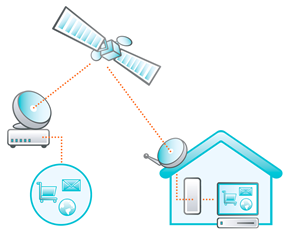
\includegraphics[scale=1]{Imagenes/Casa.png}
		\label{fig:Casa}
		%	\captionsetup{justification=raggedright,font={scriptsize,bf,it}}
		%	\caption*{fuente: \textcolor{
		%			Orange}{Tomada de Wikipedia}}
	\end{figure}
La reflexión es responsable del fenómeno de de multitrayectoria o Rayleigh y el de scattering. 

\subsection{Scattering como consecuencia de la reflexión}

El scattering es debido a las condiciones de la superficie sobre la cual cae una onda incidente, resulta un desorden de ondas son reflejadas en diferentes direcciones, como se muestra en la Figura \ref{fig:Refraccion}.
	
	\begin{figure}[h!]
		\captionsetup{justification = raggedright, singlelinecheck = false}
		\caption{Fenómeno de Scattering} 
		\centering
		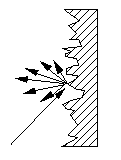
\includegraphics[scale=1]{Imagenes/Refraccion.png}
		\label{fig:Refraccion}
		%	\captionsetup{justification=raggedright,font={scriptsize,bf,it}}
		%	\caption*{fuente: \textcolor{
		%			Orange}{Tomada de Wikipedia}}
	\end{figure}



\subsection{La refracción}
Consiste en el cambio de dirección de una onda que se produce al pasar oblicuamente de un medio a otro de distinta densidad. Entre los usos o consecuencias de la refracción se tiene: \\

\begin{itemize}
	\item    La posibilidad de aprovechar este fenómeno para alcanzar puntos de comunicación tan lejanos que pueden estar más allá de la línea de vista aprovechando el paso por las capas atmosféricas con diferentes densidades.
	
%	\vspace{200px}
	\begin{figure}[h!]
		\captionsetup{justification = raggedright, singlelinecheck = false}
		\caption{Formas de refracción} 
		\centering
		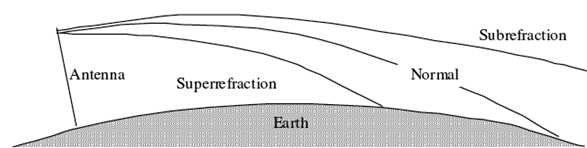
\includegraphics[scale=1]{Imagenes/Earth.png}
		\label{fig:Earth}
		%	\captionsetup{justification=raggedright,font={scriptsize,bf,it}}
		%	\caption*{fuente: \textcolor{
		%			Orange}{Tomada de Wikipedia}}
	\end{figure}
	\item  El uso de la ionosfera en sistemas de comunicación terrestres o espaciales.
	
	%\vspace{200px}
	\begin{figure}[h!]
		\captionsetup{justification = raggedright, singlelinecheck = false}
		\caption{El camino por refracción en función del ángulo de emisión} 
		\centering
		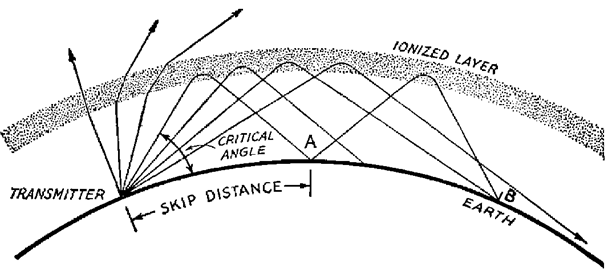
\includegraphics[scale=1]{Imagenes/Ionosfera.png}
		\label{fig:Ionosfera}
		%	\captionsetup{justification=raggedright,font={scriptsize,bf,it}}
		%	\caption*{fuente: \textcolor{
		%			Orange}{Tomada de Wikipedia}}
	\end{figure}
\end{itemize}


\subsection{La dispersión}
Ocurre cuando una onda atraviesa un medio que hace que diferentes longitudes de onda viajen a velocidades diferentes, lo cual hace también que cada longitud de onda tenga un ángulo de refracción diferente. En la Figura \ref{fig:Trian} se muestra un ejemplo para el caso de la luz. \\

\vspace{200px}
\begin{figure}[h!]
	\captionsetup{justification = raggedright, singlelinecheck = false}
	\caption{La Dispersión de la luz al pasar por un prisma} 
	\centering
	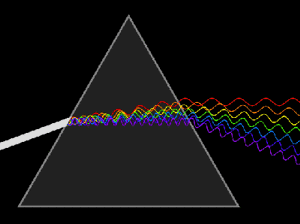
\includegraphics[scale=1]{Imagenes/Trian.png}
	\label{fig:Trian}
	%	\captionsetup{justification=raggedright,font={scriptsize,bf,it}}
	%	\caption*{fuente: \textcolor{
	%			Orange}{Tomada de Wikipedia}}
\end{figure}

Entre los usos o consecuencias de la dispersión se tiene: \\

\begin{itemize}
	\item  El efecto de la lluvia o la nubosidad en la calidad de las comunicaciones.
	
%	\vspace{200px}	
	\begin{figure}[h!]
		\captionsetup{justification = raggedright, singlelinecheck = false}
		\caption{Influencia de la lluvia en la dispesión} 
		\centering
		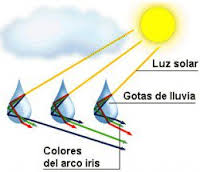
\includegraphics[scale=1]{Imagenes/lluvia.png}
		\label{fig:lluvia}
		%	\captionsetup{justification=raggedright,font={scriptsize,bf,it}}
		%	\caption*{fuente: \textcolor{
		%			Orange}{Tomada de Wikipedia}}
	\end{figure}
	
	\item  El surgimiento de interferencias indeseadas sobre una comunicación:
	
	\begin{figure}[h!]
		\captionsetup{justification = raggedright, singlelinecheck = false}
		\caption{Interferencias por Dispersión} 
		\centering
		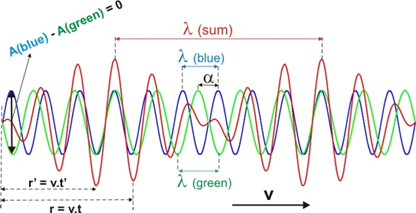
\includegraphics[scale=1]{Imagenes/Onda.png}
		\label{fig:Onda}
		%	\captionsetup{justification=raggedright,font={scriptsize,bf,it}}
		%	\caption*{fuente: \textcolor{
		%			Orange}{Tomada de Wikipedia}}
	\end{figure}
\end{itemize}
%\vspace{100px}
\subsection{La difracción}

%\vspace{5px}
\begin{figure}[h!]
	\captionsetup{justification = raggedright, singlelinecheck = false}
	\caption{La Difracción en las ondas de agua} 
	\centering
	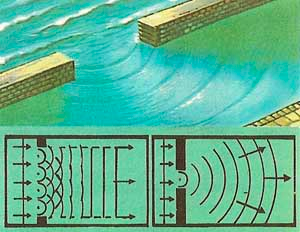
\includegraphics[scale=1]{Imagenes/Rio.png}
	\label{fig:Rio}
	%	\captionsetup{justification=raggedright,font={scriptsize,bf,it}}
	%	\caption*{fuente: \textcolor{
	%			Orange}{Tomada de Wikipedia}}
\end{figure}

Es la responsable del fenómeno conocido como sombra (shadowing), pues a un punto obstruido llega menos energía que a uno en línea de vista, como se muestra en la siguiente figura.

%	\vspace{200px}
\begin{figure}[h!]
	\captionsetup{justification = raggedright, singlelinecheck = false}
	\caption{La sombra como consecuencia de la difración} 
	\centering
	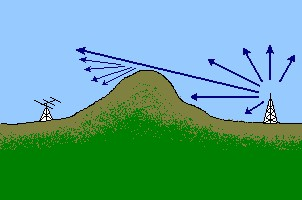
\includegraphics[scale=1]{Imagenes/Valle.png}
	\label{fig:Valle}
	%	\captionsetup{justification=raggedright,font={scriptsize,bf,it}}
	%	\caption*{fuente: \textcolor{
	%			Orange}{Tomada de Wikipedia}}
\end{figure}

\subsection{El Efecto Doppler}

Es el cambio de frecuencia que sufre una onda simplemente debido a la velocidad relativa entre los elementos que intervienen en la comunicación.\\

%\vspace{300px}
\begin{figure}[h!]
	\captionsetup{justification = raggedright, singlelinecheck = false}
	\caption{El Efecto Doppler} 
	\centering
	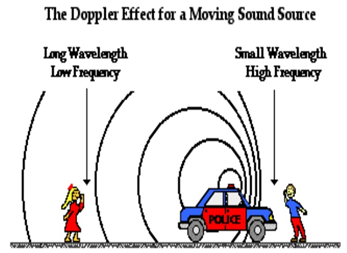
\includegraphics[scale=1]{Imagenes/Policia.png}
	\label{fig:Policia}
		\captionsetup{justification=raggedright,font={scriptsize,bf,it}}
		\caption*{fuente: \textcolor{
			Orange}{Wikipedia}}
\end{figure}

\textbf{Consecuencias del Efecto Doppler:} En un receptor digital basado en GNU Radio este efecto se traduce en que la constelación observada adquiere una velocidad proporcional a la frecuencia Doppler.

\section{La radio propagación}

La radiopropagación brinda herramientas para realizar planeación de coberturas de un sistema de radio comunicaciones. Sin embargo nuestro interés principal es conocer cómo los fenómenos de propagación pueden afectar a una señal que viaja por el canal y cuales pueden ser las medidas para contrarrestar esos efectos. \\

\subsection{La antena}
\textcolor{red}{Oscar reyes}
\textcolor{red}{[Falta. La idea es explicar lo suficiente como para que el estudiante sepa que aquí hay un elemento que no puede ignorar. Por ejemplo, el uso de una antena inadecuada puede hacer que no llegue señal, bien sea por los parámetros que la antena tiene o porque ese dañada. También puede ocurrir que no se esté apuntando hacia otras partes. Fuera de que el usuario debe tomar precauciones por la radiación que produce la antena y los posibles daños a la salud. Por lo menos debe saber si realmente está protegido. Para profundizar más, ofreceremos enlaces a la página web del libro.}\\ %\OR extensión?

La antena en el modo de transmisión puede ser vista como un conversor de una señal eléctrica a una señal electromagnética capaz de propagarse en forma de ondas electromagnéticas. Igualmente, en el modo de recepción representa una especie de sensor de las ondas electromagnéticas para expresarlas en forma eléctrica. Por sencillo que parezca esto, representa realmente la Teoría de Maxwell y su aplicación a la teoría de antenas, pero no es objetivo de este libro entrar a profundizar en estos temas. Lo que es importante tener en cuenta es que la antena tiene limitaciones expresadas principalmente en el cuanto a Ancho de Banda, su capacidad para enfocarse en una dirección, mejor conocida como la directividad de la antena o patrón de radiación de la antena y algunos coeficientes de rendimiento.\\

\subsubsection{La Potencia Isotrópica Radiada Equivalente - PIRE}
En los sistemas de Radiocomunicación, la Potencia Isotrópica Radiada Equivalente (PIRE) es la cantidad de potencia que emitiría una antena isotrópica teórica (es decir, aquella que distribuye la potencia exactamente igual en todas direcciones) para producir la densidad de potencia observada en la dirección de máxima ganancia de una antena. La PIRE tiene en cuenta las pérdidas de la línea de transmisión y en los conectores e incluye la ganancia de la antena. La PIRE se expresa habitualmente en decibelios respecto a una potencia de referencia emitida por una potencia de señal equivalente. La PIRE permite comparar emisores diferentes independientemente de su tipo, tamaño o forma. Conociendo la PIRE y la ganancia de la antena real es posible calcular la potencia real y los valores del campo electromagnético.



\begin{equation} \label{equ_pire}
PIRE=P_{T}-L_{c}+G_{a}	 				
\end{equation}

donde $ PIRE $ y $P_{T}$  (potencia del transmisor) son $dBm$, las pérdidas del cable ($L_{c}$) están en $d$, y la ganancia de la antena ( $G_{a})$  se expresa en $dBi$, relativos a la antena de referencia isotrópica.

El siguiente ejemplo utiliza dBm, aunque también es correcto utilizar dBW. Los Decibelios son una forma muy práctica de expresar la relación entre dos cantidades. dBm utiliza una referencia de 1 mW y dBW 1 W.

\begin{equation} \label{equ_dbm}
dBm=10\log \left({\frac {\text{potencia}}{1\,\mathrm {mW} }}\right) 				
\end{equation}

y

\begin{equation} \label{equ_dbw}
dBW=10\log \left({\frac {\text{potencia}}{1\,\mathrm {W} }}\right) 				
\end{equation}



Por ejemplo, una transmisión de 50 W es lo mismo que 17 dBW o 47 dBm.

\begin{equation} \label{equ_dbwdos}
\displaystyle 16.9897\,\mathrm {dBW} =10\log \left({\frac {50\,\mathrm {W} }{1\,\mathrm {W} }}\right) \\
\end{equation}

La PIRE se utiliza para estimar el área en el que la antena puede dar servicio y coordinar la radicación entre transmisores para que no se solapen las coberturas.
%%%%%%%%%%%%%%%%%%%%%%%%%%%%%%%%%%%%%%%%%%%%%%%%%%%

\subsection{La Densidad de Flujo de Potencia}

En un punto de interés, en campo lejano, la Densidad de Flujo de Potencia (PFD, del inglés Power Flux Density) está dada por el producto cruz entre los vectores $\overline{E}$ y $\overline{H}$:

\begin{equation} \label{equ_cuarenta_uno}
	 |\overline{S}|=|\overline{E} x \overline{H}|=|\overline{E} | |\overline{H}| sin \theta
\end{equation}

Donde $\overline{S}$ representa la PFD, $\overline{E}$  el campo eléctrico, $\overline{H}$ el campo magnético y $\theta$=90º el ángulo entre $\overline{E}$ y $\overline{H}$ para el caso del campo lejano. De modo que, para el campo lejano,  se puede reescribir  como: 

\begin{equation} \label{equ_cuarenta_dos}
	|\overline{S}|=|\overline{E} | |\overline{H}|
\end{equation}


Resulta importante apuntar que, desde el punto de vista de la propagación del campo eléctrico, el vacío (el espacio libre) tiene una impedancia conocida como impedancia característica del espacio libre y es igual a: 

\begin{equation} \label{equ_cuarenta_tres}
	 \eta_{0} = \dfrac{|\overline{E} |}{|\overline{H}|} = \sqrt{\dfrac{\mu_{0}}{\varepsilon_{0}}}= 120\pi \Omega \approx 337\Omega 
\end{equation}

Esta relación se conoce como la ley de Ohm para los campos electromagnéticos, donde $\mu_{0}=1,26 10-6H/m$ es la permeabilidad magnética del espacio libre; $\varepsilon_{0}=8,85 10-12F/m$ es la permitividad eléctrica del espacio libre. Como consecuencia, la PFD promediada guarda una relación con el valor RMS E de la intensidad del campo eléctrico $\overline{E}$ , en un Punto de interés  (PoI, del inglés Point of Interés), similar a la que existe entre la potencia promedio P de una señal de voltaje y su valor RMS: 

\begin{equation} \label{equ_cuarenta_cuatro}
	  S= \dfrac{E^{2}}{\varepsilon_{0}}
\end{equation}

En campo lejano es posible obtener el valor RMS H de la intensidad del campo magnético $\overline{H}$ a partir del eléctrico y viceversa de la siguiente manera:

\begin{equation} \label{equ_cuarenta_cinco}
	  H= \dfrac{E}{\varepsilon_{0}}, E=\varepsilon_{0}H
\end{equation}

Cuando se realizan mediciones de espectro, las emisiones pueden provenir de diferentes direcciones. Por eso, en algunos casos puede ser necesario conocer los aportes a E y H en las direcciones de las 3 direcciones del espacio físico, tridimensional:

\begin{equation} \label{equ_cuarenta_seis}
E = \sqrt{E_{x}^{2}+E_{y}^{2}+E_{z}^{2}} 
\end{equation}

\begin{equation} \label{equ_cuarenta_siete}
 H = \sqrt{H_{x}^{2}+H_{y}^{2}+H_{z}^{2}} 
\end{equation}

\subsection{Fenómeno de desvanecimiento. Pérdidas por Espacio Libre. Ecuación de Friss}

Se conoce como desvanecimiento en espacio libre (free space path loss) la pérdida de potencia captada por un receptor en función de la transmitida por un emisor, cuando no existe ningún obstáculo para la propagación, como ocurre en el cosmos o Espacio Libre (Free Space). Conocer la regla de cálculo de este tipo de pérdidas es de gran utilidad ya que sirven como una primera aproximación para las mediciones de la potencia que puede llegar a un receptor ubicado a una cierta distancia del emisor. \\



\subsubsection{La densidad de Flujo de Potencia en campo lejano}

Un caso teórico de enorme importancia consiste en el supuesto de contar con una fuente isotrópica que radia una potencia promedio $P_t$. La cuestión es que a medida que la onda se aleja a una distancia d, esa potencia se distribuye en el área de una  esfera $A$ de radio $d$ que se conforma alrededor de la fuente. Precisamente, como la potencia se distribuye en un área, se puede hablar de la Densidad de flujo de potencia $S_d$ por área.  Teniendo en cuenta que el área de la esfera es.\\

\begin{equation} \label{equ_cuarenta_ocho}
	 A_{es}= 4 \pi d^{2}
\end{equation}

La PFD es:

\begin{equation} \label{equ_cuarenta_nueve}
	S_{d}= \dfrac{P_t}{A_{es}}= \dfrac{P_t}{4 \pi d^{2}} Watt/m^{2}
\end{equation}

\subsubsection{El área efectiva de una antena }

En un área elemental de interés para la recepción $A_r (m^{2})$, como se muestra en la figura \ref{fig:Antena} , se recibe una potencia elemental $P_r$

$P_r= S_d A_r$

%\vspace{300px}
%	\setcounter{figure}{94}
\begin{figure}[h!]
	\captionsetup{justification = raggedright, singlelinecheck = false}
	\caption{Elemento de Área donde puede localizarse el receptor} 
	\centering
	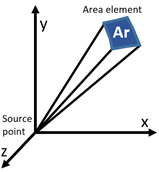
\includegraphics[scale=1.1]{Imagenes/Antena.png}
	\label{fig:Antena}
	%	\captionsetup{justification=raggedright,font={scriptsize,bf,it}}
	%	\caption*{fuente: \textcolor{
	%			Orange}{Tomada de Wikipedia}}
\end{figure}


Una antena, vista como un sensor, debe abarcar cierta área. Por esta razón, la capacidad de una antena para captar una potencia $P_r$ está asociada a un área que se conoce como el área efectiva Aeff de la antena o apertura efectiva de la antena.

\subsubsection{Una antena isotrópica} 

Una antena de recepción isotrópica ideal es aquella que irradia (o recibe) por igual en todas direcciones y tiene un área efectiva $A_{effiso}$ bien conocida que sirve como patrón para caracterizar otras antenas:

\begin{equation} \label{equ_cincuenta}
	A_{effiso} =\dfrac{\lambda^{2}}{4 \pi}= \frac{c^{2}}{4\pi f^{2}} 
\end{equation}

Así, el área efectiva está en función de la longitud de onda y disminuye conforme aumenta la frecuencia. Por esa razón, desde el punto de vista de una antena isotrópica, las ondas de mayor frecuencia se atenúan más rápidamente que las de menor. Por lo tanto, la potencia que puede captar una antena isotrópica es: \\

\begin{equation} \label{equ_cincuenta_uno}
	P_r= S_d A_{effiso}= S_d \dfrac{\lambda^{2}}{4 \pi} =  P_t \left(\dfrac{\lambda}{4 \pi d}\right)^{2}
\end{equation}

\subsubsection{Ecuación de Friis}

Es claro que a medida que una  señal de radio se propaga en la distancia, su energía se va esparciendo en un área cada vez mayor, lo cual va a ser percibido por un equipo receptor como un desvanecimiento, que en condiciones ideales, de espacio libre y usando antenas isotrópicas en transmisión y recepción, se expresa por el coeficiente:

\begin{equation} \label{equ_cincuenta_dos}
		 l_{fs}=  \left(\dfrac{4 \pi d}{\lambda} \right)  ^{2}
\end{equation}

Este coeficiente se conoce en inglés como Free Space Path Loss, en español como  Desvanecimiento en Espacio Libre o Pérdidas en Espacio Libre.\\
En función de la frecuencia tenemos que:

\begin{equation} \label{equ_cincuenta_tres}
	 l_{fs}=  \left(\dfrac{4 \pi df}{c} \right)  ^{2}
\end{equation}

Donde $c$ es la velocidad de la luz. \\
Muchas veces el Desvanecimiento en Espacio Libre se usa en dB. \\


\begin{equation} \label{equ_cincuenta_cuatro}
	 l_{fs}(dB)=  10log(lf_{s})
\end{equation}

\begin{equation} \label{equ_cincuenta_cinco}
	 l_{fs}(dB)=  20log\left(\dfrac{4\pi}{0.3(km/\mu seg)}\right)+ 20log(d(km)f(MHz))
\end{equation}

Entonces se obtiene la expresión más conocida para las pérdidas en espacio libre: \\
\begin{equation} \label{equ_cincuenta_seis}
	 l_{fs}(dB)=  32.4+20log(f)(MHz)+20log(d)[km]
\end{equation}

No hay que olvidar que aún con estos ajustes de ganancia, esta ecuación corresponde al caso ideal de propagación en espacio libre.  En un caso real, para las comunicaciones terrenales las pérdidas en espacio libre son apenas una referencia a la cual se suman otras pérdidas como las pérdidas por irregularidad del terreno o las pérdidas por otros aspectos como la altura del transmisor, la del receptor, si el ambiente de propagación que puede ser urbano, suburbano, rural, abierto o porque que hay tipos especiales de vegetación o falta de ella: \\

\begin{equation} \label{equ_cincuenta_siete}
	L(dB)=L_{reference}+L_{Terrain Irregularity}+L_{Environment}
\end{equation}

En condiciones de espacio libre, la potencia recibida se puede calcular como: \\

\begin{equation} \label{equ_cincuenta_ocho}
	 P_r=\frac{P_t}{l_{fs}}=P_t\left(\frac{\lambda}{4\pi d}\right)^{2}
\end{equation}

Si las antenas no son isotrópicas se les puede realizar ajuste, con lo cual se llega a la forma más común de la Ecuación de Friis:

\begin{equation} \label{equ_cincuenta_nueve}
	 P_r= P_t G_t G_r\frac{P_t}{l_{fs}}=P_t\left(\frac{\lambda}{4\pi d}\right)^{2}
\end{equation}

\textbf{Nota:} $G_r$ está multiplicando a la derecha, entonces está dividiendo a la izquierda, luego $\frac{P_r}{G_t}= \dfrac{P_tG_r}{l_{sf}}$. Eso es correcto, pues la ganancia en la parte receptor contribuye a elevar el área efectiva de la antena receptora y esa área está a la derecha de la ecuación.
Entonces la potencia recibida se calcula como: \\

\begin{equation} \label{equ_sesenta}
	P_r(dB)=P_t(dB)+G_t(dB)+G_r(dB-L(dB)
\end{equation}

\subsection{Propagación en Línea de Vista. Distribución de Rice}
En el mundo real, la potencia que se recibe está oscilando todo el tiempo y el comportamiento de esas oscilaciones depende de varios factores. Uno de ellos es que la recepción se realice en línea de vista (LOS, del inglés Line of Sight), donde, aunque influyen muchos fenómenos de las ondas, predomina la señal que llega directamente de la antena transmisora, pero es influenciada por débiles señales que llegan reflejadas de diferentes obstáculos. \\
%\vspace{200px}
\begin{figure}[h!]
	\captionsetup{justification = raggedright, singlelinecheck = false}
	\caption{Fenómeno de Multitrayectoria} 
	\centering
	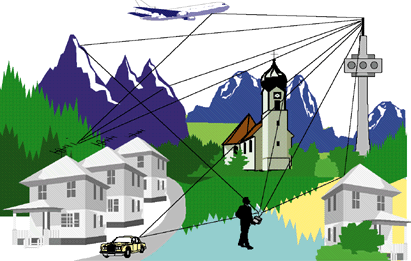
\includegraphics[scale=1]{Imagenes/Edificio.png}
	\label{fig:Edificio}
	%	\captionsetup{justification=raggedright,font={scriptsize,bf,it}}
	%	\caption*{fuente: \textcolor{
	%			Orange}{Tomada de Wikipedia}}
\end{figure}

En la siguiente figura se muestra la imagen que resulta al medir la potencia de la señal RF para este caso. \\
%\vspace{100px}
\begin{figure}[h!]
	\captionsetup{justification = raggedright, singlelinecheck = false}
	\caption{Nivel de potencia medida en LOS} 
	\centering
	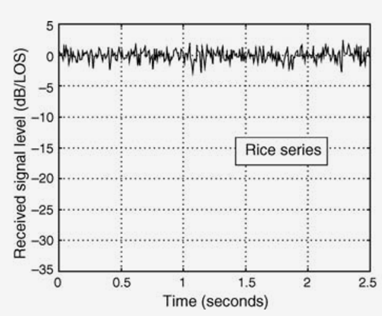
\includegraphics[scale=1]{Imagenes/Medidor.png}
	\label{fig:Medidor}
		\captionsetup{justification=raggedright,font={scriptsize,bf,it}}
		\caption*{fuente: Tomado de F. Pérez Fontán\textbf{Nota:}Esta no es la señal recibida sino lo que entrega un medidor de nivel de potencia} 
\end{figure}

Desde el punto de vista de los Procesos estocásticos, el nivel de señal que se recibe en línea de vista sigue la distribución de Rice.\\

El efecto de Rice se observa no solo en LOS, sino también en algunos casos ocurre en No Línea de Vista (NLOS), por ejemplo, cuando un obstáculo puede ser visto como un fuerte reflector de la señal, lo cual ocurre a menudo en las comunicaciones móviles cuando la señal llega reflejada de una superficie suave de un edificio que si tiene LOS. \\

\subsection{Pérdidas Propagación en Línea de Vista. Distribución de Rice}

Cuando no hay línea de vista (NLOS), en el nivel de señal recibido predominan los débiles aportes de energía que se reciben de manera indirecta, principalmente por el efecto de multitrayectoria, es decir la multitud de ondas que llegan al receptor, recorriendo diferentes distancias, debido al efecto de la reflexión que las  ondas sufren al encontrarse con diferentes obstáculos en su propagación. Estos obstáculos pueden ser edificios, señales de tráfico, árboles, personas y hasta gatos. La suma de las señales que llegan de esos obstáculos causa en el receptor distorsiones tanto constructivas como destructivas. \\

Cuando predomina el efecto de multitrayectoria, la señal RF medida en el receptor muestra una combinación de variaciones rápidas (Fast Fading) y lentas (Slow Fading), como se muestra en la figura siguiente. \\ 

%\vspace{200px}
\begin{figure}[h!]
	\captionsetup{justification = raggedright, singlelinecheck = false}
	\caption{Niveles de potencia medidos en un punto donde se presenta el Efecto de Rayleigh} 
	\centering
	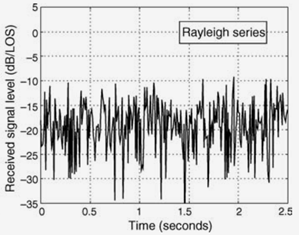
\includegraphics[scale=1]{Imagenes/Rayleigh.png}
	\label{fig:Rayleigh}
	\captionsetup{justification=raggedright,font={scriptsize,bf,it}}
		\caption*{Fuente: Tomado de F. Pérez Fontán. Nota: esta no es la señal recibida sino lo que entrega un medidor de nivel de potencia} 
\end{figure}

Pero el efecto de Rayleigh no solo se observa en condiciones de NLOS, también se observa en un vehículo que se mantiene en LOS, alejándose de la fuente, mientras se desplaza por una zona rural con geografía variable, como se muestra en la siguiente figura. \\

\vspace{200px}
\begin{figure}[h!]
	\captionsetup{justification = raggedright, singlelinecheck = false}
	\caption{Efecto de Rayleigh en un caso de LOS} 
	\centering
	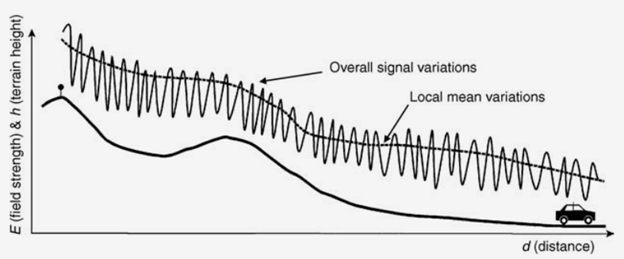
\includegraphics[scale=1]{Imagenes/Field.png}
	\label{fig:Field}
	\captionsetup{justification=raggedright,font={scriptsize,bf,it}}
	\caption*{Fuente: Tomado de F. Pérez Fontán. Nota: Esta no es la señal recibida sino lo que entrega un medidor de nivel de potencia. En esta figura no se muestra el desvanecimiento por la distancia, que puede compensarse mediante un sistema de amplificación automática.} 
\end{figure}

Las variaciones rápidas (Fast Fading or Fast Variations or short term variations) son debidas al efecto de multitrayectoria en sí, mientras que las lentas (Slow Fading or Slow Variations or long-term variations) son debidas principalmente efecto de desvanecimiento por sombra (shadowing), el cual, a su vez es una consecuencia de refracción de las ondas con respecto a las montañas y otros obstáculos. El anterior es el peor escenario, se encuentra en ambientes urbanos densos de altas edificaciones, pero también en ambientes rurales donde la señal es obstruida por densa masa de árboles. La siguiente figura muestra lo que pasaría si las variaciones lentas son promediadas, (parte izquierda) y las variaciones rápidas que resultan al restar a la señal las variaciones lentas (parte derecha). \\

\begin{figure}[h!]
	\captionsetup{justification = raggedright, singlelinecheck = false}
	\caption{El Desvanecimiento lento} 
	\centering
	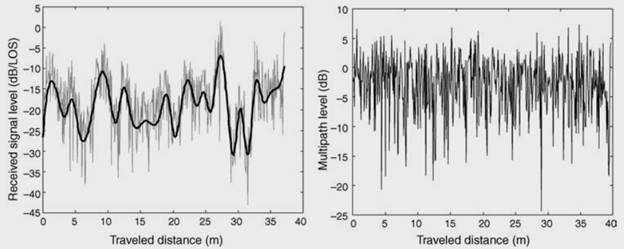
\includegraphics[scale=1]{Imagenes/Distancia.png}
	\label{fig:Distancia}
	\captionsetup{justification=raggedright,font={scriptsize,bf,it}}
	\caption*{Fuente: tomado de F. Pérez Fontán} 
\end{figure}

\section{Equipo de Laboratorio y de medida}

\subsection{El osciloscopio}
\textcolor{red}{[Falta: Oscar Reyes]} % \OR Algún osciloscopio en particular? Qué tan general??

[Falta. La idea es brindar una pequeña explicación y un enlace a la pagina web para que vean un curso sobre el uso correcto del equipo. Hay que dejar claro, que al igual que los USRP son equipos que hay que conocer muy bien y darle un buen uso para que no se dañen. Es importante incluir unas recomendaciones de uso aquí.]

\subsection{El Analizador de Espectros}

Aunque se dice que el ERE es un recurso intangible, que no se puede ver, ni oler, ni pesar, en realidad es posible apreciarlo mediante el uso de un Analizador de Espectros.\\

El Analizador de espectros se basa en el uso de un banco de filtros, cada uno de los cuales está acotado a un ancho de banda lo más angosta posible centrado en una frecuencia diferente a los demás, de modo que entre todos los filtros sea posible cubrir un ancho de banda de interés, centrado en una cierta frecuencia intermedia (FI). El uso de un receptor superheterodino es clave para poder mover a la FI el espectro de la señal que se desea analizar. Una pantalla toma la salida de cada filtro para crear la imágen espectral que consiste en amplitudes de señal distribuidas sobre el eje de las frecuencias. El espectro que muestra el Analizador de espectros es dinámico ya que corresponde a al comportamiento instantáneo de una señal, a diferencia de los métodos teóricos usados para obtener el espectro, donde una señal es muchas veces analizada en toda su extensión. También es posible obtener un espectro promediado y un espectro pico como imágenes algo más estáticas. \\

Los analizadores de espectros pueden ser construidos también con tecnología digital que imita al banco de filtros por lo que tienen la misma apariencia.\\
\textcolor{red}{[Falta: Oscar Reyes]} % \OR qué se espera, qué extensión? enfocado a uso, a estructura....?


\subsection{El Analizador Vectorial de Redes}
\textcolor{red}{Falta:Oscar reyes }\\


\subsection{El Generador Vectorial de Señales}
\textcolor{red}{Falta:Oscar reyes }\\
\subsection{El Analizador Vectorial de Señales}
\textcolor{red}{Falta: Oscar reyes }\\


\subsection{El Analizador Vectorial de Señales}
\textcolor{red}{Falta: Oscar Reyes }\\

\subsection{Medidor de RNI}
\textcolor{red}{Falta: Oscar Reyes}\\

\section{Medición de potencia propagada}

El espacio libre se refiere al caso ideal en que las ondas se propagan libres de cualquier obstáculo como sucedería por ejemplo en el cosmos. Pero tiene una gran utilidad también para condiciones terrestres, pues brinda la posibilidad de realizar una aproximación gruesa, que puede ser complementada con factores terrestres si resulta necesario obtener cálculos más precisos. \\

\subsection{Valor RMS y Potencia Promedio}

En la práctica, aunque el equipo de medición se ubique en un punto de interés (PoI) fijo, la amplitud de las ondas que inciden en el equipo varían aleatoriamente, debido a la información que transportan y a todos los fenómenos que ocurren en el canal inalámbrico. Consecuentemente varía en el tiempo la señal de voltaje que entrega la antena del equipo de medición. Por esta razòn, es necesario usar promedios de tiempo. Resulta entonces pertinente recordar la definición de valor RMS que uno de esos promedios aplicados a una señal aleatoria de voltaje v(t): \\

\begin{equation} \label{equ_sesenta_uno}
	 V_{RMS} = \lim_{Taver \to \infty} \sqrt{\dfrac{1}{Taver} \int_{0}^{Taver} |V(t)|^{2} dt} 
\end{equation}

Otro promedio de tiempo importante es el de potencia promedio, que se puede obtener a partir del valor RMS asì: \\

\begin{equation} \label{equ_sesenta_dos}
	 P = \dfrac{{V_{RMS}}^{2}}{Z} = \lim_{Taver \to \infty} \dfrac{1}{Z Taver} \int_{0}^{Taver} |V(t)|^{2} dt 
\end{equation}

Donde Z es la impedancia del medio en el cual viaja la señal . \\

\subsection{Campo cercano versus campo lejano. }

En la radio propagación de las ondas electromagnéticas se distinguen el campo cercano y el campo lejano. Lo importante a tener en cuenta en las mediciones es que, a una distancia mayor a 3 longitudes de onda, es posible considerar que el frente de una onda electromagnética que puede ser capturado por una antena es plano y los campos eléctricos y el magnético son ortogonales entre sí. No ocurre lo mismo a distancias menores y, por lo tanto, se requieren equipos especializados para la medición. El primer caso corresponde al campo lejano y el segundo al cercano. Los equipos de medición que provee la industria para frecuencias altas en campo lejano permiten medir el campo eléctrico E(V/m) o el campo magnético H(A/m) o la densidad de flujo de potencia $S(W/m^{2})$. \\

\subsection{Factor de antena} 

Una de las grandes dificultades para la realización de trabajos de campo radica en el diseño de un equipo capaz de medir la intensidad de un campo eléctrico incidente $e_i (t)$ en un PoI, empleando un receptor de ondas RF y una antena. La antena es usada como un sensor de la intensidad del campo eléctrico en el PoI, o más bien como un transductor de ese campo a una señal eléctrica aleatoria de voltaje $v_r (t)$ que tiene un valor RMS $V_r$. De modo que la potencia promedio es:   \\


\begin{equation} \label{equ_sesenta_tres}
	 P_R= \dfrac{V_r^{2}}{Z_{Ant}}
\end{equation}

Donde $Z_{Ant}$ es impedancia de la antena receptora. El Factor (AF) de la antena receptora es precisamente el coeficiente de proporcionalidad entre  $E_i$ y $V_r$:

\begin{equation} \label{equ_sesenta_cuatro}
	  A_{fR} = \dfrac{E_i}{V_r}
\end{equation}

Por esta razón es necesario conocer el AF para determinar la intensidad del campo eléctrico incidente a partir $V_r$. Además, con los conceptos ya vistos, puede deducirse que  $V_r$ está relacionado con el área efectiva de la antena así: \\

\begin{equation} \label{equ_sesenta_cinco}
	 \dfrac{{V_{r}}^{2}}{Z_{Ant}} = S_{r} A_{eff}= \dfrac{{E_{i}}^{2}}{120 \pi} * \dfrac{\lambda^{2}}{4\pi} G_{r}
\end{equation}

Por lo tanto, el factor de antena puede hallarse a partir de los parámetros de la antena y es función de la longitud de onda: \\
        
\begin{equation} \label{equ_sesenta_sies}
	  A_{fR} = \dfrac{E_i}{V_r} = \sqrt{\dfrac{480\pi^{2}}{Z_{Ant} \lambda^{2}G_{r}}}
\end{equation}

Esta fórmula sugiere conocer simplemente la ganancia de la antena receptora y la impedancia de la antena, mientras se hace variar la frecuencia o la longitud de onda en el rango de interés. También es posible encontrar una expresión para el factor de antena a partir de la potencia transmitida así: \\

\begin{equation} \label{equ_sesenta_siete}
S_{r}=\dfrac{P_{r}}{A_{eff}}= \dfrac{P_{t}G_{t}G_{r}}{A_{eff}} (\dfrac{\lambda}{4 \pi r})^{2}=\frac{P_{t}G_{t}}{4\pi r^{2}} 
\end{equation}

\begin{equation} \label{equ_sesenta_ocho}
{E_{i}}^{2} = S_{r}120\pi =30 \dfrac{P_{t} G_{t}}{r^{2}}
\end{equation}

Sustituyendo en $A_{fR} = \dfrac{1}{V_r}\sqrt{30P_{r}G_{t}}$ Esta fórmula sugiere la realización de un experimento usando un transmisor de potencia y ganancia conocida, y ubicando un receptor a una distancia $r$ también conocida, para medir $V_r$ y calcular el factor de antena según  \textcolor{orange}{(21)}. \\

La figura \ref{fig:Factor-antena} resumen las relaciones de mayor interés, donde se observa que: la antena transmisora también tiene un factor de antena $A_{fT}$, el cual también puede entrar a jugar un papel importante en las mediciones. \\ 

%\vspace{200px}
%\setcounter{figure}{126}
\begin{figure}[h!]
	\captionsetup{justification = raggedright, singlelinecheck = false}
	\caption{El factor de antena en la práctica} 
	\centering
	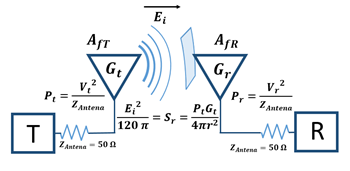
\includegraphics[scale=1]{Imagenes/Factor-antena.png}
	\label{fig:Factor-antena}
	%	\captionsetup{justification=raggedright,font={scriptsize,bf,it}}
	%	\caption*{fuente: \textcolor{
	%			Orange}{Tomada de Wikipedia}}
\end{figure}

\subsection{Parámetros S11 de las antenas}

El parámetro $S_{11}$ de una antena puede jugar también un papel importante en las mediciones de RNI. En este sentido, lo que debe tenerse en cuenta es que $S_{11}$ representa la relación entre la potencia reflejada por la antena u la aceptada y por eso se conoce también como coeficiente de reflexión o pérdidas de retorno de la antena. Por ejemplo, si $S_{11}=0dB$, toda la potencia es reflejada de la antena y nada es recibido. Pero si $S_{11}=-10 dB$ significa que si llegan 3 dB a la antena, -7dB es lo reflejado por la antena y lo demás es lo aceptado. 

\section{El Espectro Radioeléctrico}
El espectro radioeléctrico (ERE) es un término usado principalmente por las autoridades para hacer referencia a ese valioso recurso que permite el desarrollo de las comunicaciones inalámbricas.
Existen dos tipos de autoridades: las nacionales y las internacionales. A nivel internacional se tiene la Unión Internacional de Telecomunicaciones (UIT), donde se encuentra el sector de radiocomunicaciones (UIT-R). Las principales normas que \
rigen el ERE a nivel internacional están plasmadas en un acuerdo de carácter vinculante para todos los piases conocido como el Reglamento Internacional de Radio (RR, del inglés, Radio Regulations). A nivel de cada país, se tiene un documento que adapta el RR a las condiciones del \
país, en el caso de Colombia se conoce como el CNAB (Cuadro Nacional de Atribución de Bandas de Frecuencia). A continuación se resaltan la información del RR que resulta relevante para los propósitos del presente libro.

\subsection{Clasificación de las ondas de radio}

\textcolor{red}{[Falta. la idea es mostrar que las ondas electromagnéticas tienen las mismas cualidades de cualquier onda, pero que también hay aspectos especiales como:}  \\
 
 \begin{itemize}
	
	\item  No necesitan de un medio. El medio es el vació\\
    \item  La ecuación de Friss, que depende de la frecencia y la velocidad de la luz.
    \item  Que las ondas de radio, son en realidad una porción del espectro electromagnético.\\
    \item  Que todo lo anterior hace que sobre el planeta tierra las ondas tengan diferentes formas de propagación como: la ionosfera, en forma curvada, en línea recta, las espaciales, usando satélites, etc.\\
    \item  Que el ERE tienen una clasificación global en: ELF, SLF, ULF, VLF,LF, MF, HF, VHF, UHF, SHF, EHF]. tambien la clasificación en términos de la logitud de ondas como: ondas, larga, onda corta, etc.\\
\end{itemize}

\subsection{Gestión Internacional del Espectro}
\textcolor{red}{Esta es una buena fuente: https://www.itu.int/en/ITU-D/Regional-Presence/Americas/Documents/EVENTS/2016/15532-MX/D1-S2-1.pdf}
\subsubsection{La UIT y la UIT-R}

\textcolor{red}{Falta. La idea es presentar un resumen y luego mostrar enlaces a fuentes más completas.
NOTA: solo incluir no que un estudiante requiere para el curso. Lo demás, solo se referencia.}

\subsubsection{El Reglamento de Radiocomunicaciones}

\subsubsection{Los servicios de radiocomunicaciones}

El RR define ante todo los diferentes servicios de radio, las bandas de frecuencias que tienen asignadas y las condiciones en que pueden usar esas bandas. son 2 los grandes tipos de servicios:
    
\begin{itemize}
	\item   Terrenales. Son los que tienen lugar en el planeta tierra. Son 3:
    
    \begin{itemize}
	    \item  Servicios terrestres.
        \item  Servicios aeronáuticos.
        \item  Servicios marítimos.
    \end{itemize}
    
    \item  Espaciales. Los que tienen lugar fuera del planeta.
    
    	\begin{itemize}
	    	\item  Servicios satelitales
        	\item  Otros.
    	\end{itemize}
 
 	\item  Cada uno de los anteriores servicios pueden ser de tipo:
		\begin{itemize}
			\item  Servicio Fijo
    		\item  Servicio móvil
		\end{itemize}
\end{itemize}        

Para conocer con mayor profundidad estos temas, puede consultar los materiales disponibles en línea así:
\begin{itemize}
	\item   Sitio Web del libro, sección ERE 
	\item  Este es el enlace directo:
	\url{https://sites.google.com/saber.uis.edu.co/Libro/m/ERE}
\end{itemize}

\subsection{La Gestión Nacional del especto}

\textcolor{red}{Falta. La idea es presentar un resumen y enlaces a las fuentes disponibles. Es importante que estudiante conozca: las autoridades de regulación,las principales leyes y normas, pero sobre el todo el Cuadro Nacional de Atribución de Bandas de Frecuencia (CNABF), también las herramientas de consulta disponibles para conocer la ocupación del ERE.} \\

\textbf{NOTA: solo incluir no que un estudiante requiere para el curso. Lo demás, solo se referencia} \\

\subsubsection{El Ecosistema de la gestión del ERE}
\subsubsection{Autoridades de regulación}
\subsubsection{El CNABF}

%%%%%%%%%%%%%%%%%%%%%%%%%%%%%%%%%%%%%%%%%%

\section{Los modelos de capas para representar sistemas de comunicaciones}

Cualquier sistema de comunicaciones, por muy complejo que parezca, puede ser fácilmente representado mediante un modelo de capas- Esto aplica no solo en las telecomunicaciones, sino en cualquier otro sistema. Esto es debido a que, por naturaleza, la comunicación se da de manera elemental a diferentes niveles. Por ejemplo, en una empresa que vende artículos nacionales e importados pueden darse los siguientes niveles de comunicación, la que se da entre: el vendedor y el cliente; los vendedores y su jefe de ventas; los jefes de venta y su gerente; el gerente y las empresas proveedoras. En cada caso, se usa una forma especial de comunicación que puede involucrar formas de relación, términos especiales y hasta temas especiales.\\

En uso de modelos de capas en el presente libro cobra sentido por la gran cantidad de elementos que pueden llegar a formar parte de un sistema de radiocomunicaciones. Las ventajas se pueden resumir en los siguientes puntos. Permite:\\

\begin{itemize}
	\item[$\bullet$] Ordenar los elementos del sistema. Cuando no se usan capas, los componentes de un sistema de comunicaciones se parece a un ejército en el campo de batalla, donde todo funciona bien, pero resulta dificil de comprender cómo operan los diferentes mandos. Al usar el modelo de capas el sistema de comunicaciones se parece más bien a un desfile militar, donde al frente están los generales, luego los coroneles y así sucesivamente hasta llegar a los soldados.  
	\item  Reducir cuando sea necesario, el número de elementos del sistema, por ejemplo agrupando elementos en capas que encierran un mayor grupo de funcionalidades
    \item[$\bullet$] Construir un sistema funcional con funciones elementales, pero que puede ir creciendo con nuevas capas hasta llegar a ser tan complejo como sea necesario.
    \item[$\bullet$] Probar las funcionalidades de un sistema a nivel de una o algunas capas. Esto equivale a decir que es posible aislar algunas capas del sistema de comunicaciones con el fin de realizar cualquier tipo de pruebas, por ejemplo, para determinar en qué capa se puede estar presentando una falla.
\end{itemize}

Existen modelos de capas estandarizados, muy bien documentados que pueden ser usados para intercambiar ideas y conocimientos entre ingenieros y demás expertos en telecomunicaciones. Ejemplo de ellos son:
\begin{itemize}
	\item[$\bullet$] \textbf{El modelo OSI} Explicar los sistemas de comunicaciones de datos usando ocho capas. Así, un sistema particular de datos puede tener más o menos número de capas, pero a la hora de llevarlo a una discusión, siempre resulta posible presentar el sistema como el compuesto de ocho capas.
    \item[$\bullet$] \textbf{El modelo IP} IP se refiere al Protocolo de Internet, del inglés Internet Protocol. Se refiere a todo el conjunto de protocolos que se usan en las redes IP.
    \item[$\bullet$] \textbf{Otros.} La Unión Internacional de Telecomunicaciones (UIT) usa modelos para explicar diferentes sistemas de comunicaciones, como por el ejemplo para explicar el sistema de Telecomunicaciones Móviles internacionales (IMT, del inglés International Telecommunication Union), el Internet de las cosas (IoT, del inglés Internet of Things).
\end{itemize}

Los que usaremos en el presente libro no son modelos de capas recocidos, simplemente adaptados a nuestras necesidades que algunas veces son de diseño otras de documentación o simplemente de tipo pedagógico. \\

Para comenzar, vamos a revisar el modelo de capas que corresponde al sistema de comunicaciones que se da en el transporte aéreo. Con la creación de las aeronaves, se creó el sistema más sencillo usado en el transporte aéreo: la posibilidad de enlazar dos ciudades. \\
El modelo de capas que representa esta posibilidad es el que se tiene en la Figura \ref{fig:modelo_aviacion}. El avión aprovecha un pequeño corredor del Espacio Aéreo; en el aeropuerto convergen las personas y las aeronaves. \\

%\vspace{200px}
\begin{figure}[h!]
	\captionsetup{justification = raggedright, singlelinecheck = false}
	\caption{Modelo de capas para el transporte aéreo entre dos ciudades} 
	\centering
	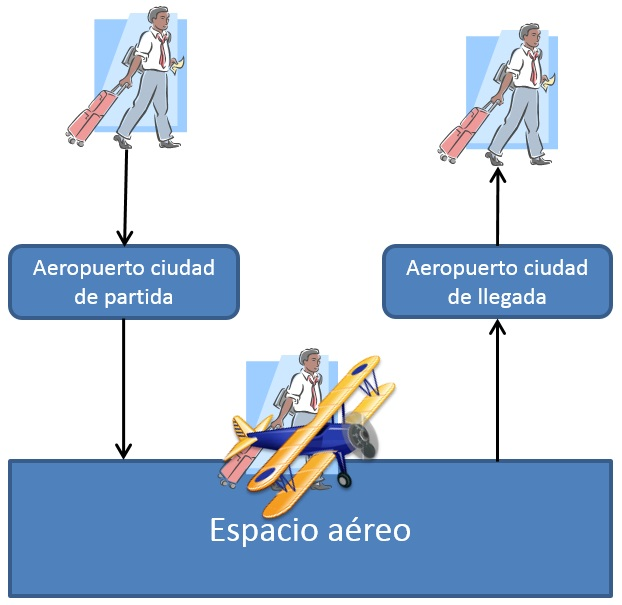
\includegraphics[scale=0.6]{Imagenes/modelo_aviacion}
	\label{fig:modelo_aviacion}
	%		\captionsetup{justification=raggedright,font={scriptsize,bf,it}}
	%		\caption*{fuente: http://superkuh.com/rtlsdr.html}
\end{figure}

Con el tiempo, ese sistema de comunicación evolucionó hasta convertirse en una compleja red que une miles de ciudades, como la que aparece en Figura \ref{fig:AirTrafficNetwork}, siempre respetando los lineamientos que imponen las autoridades encargadas de la administración del espacio aéreo. \\

%\vspace{200px}

\begin{figure}[h!]
	\captionsetup{justification = raggedright, singlelinecheck = false}
	\caption{Red de Transporte Aéreo} 
	\centering
	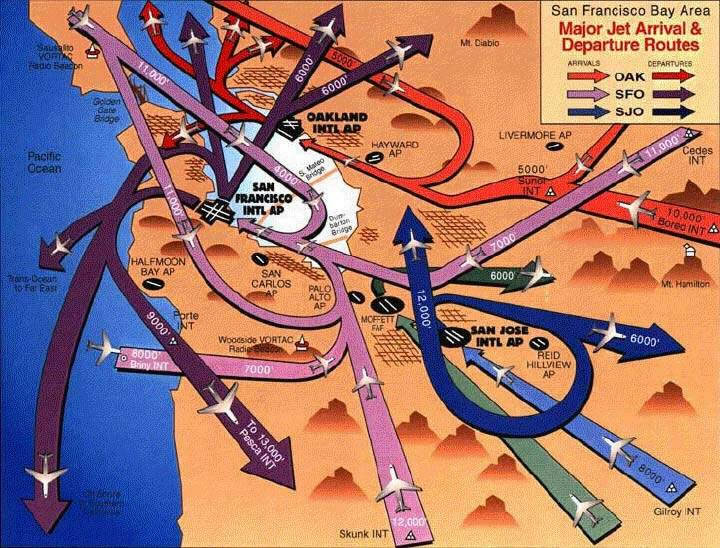
\includegraphics[scale=0.4]{Imagenes/AirTrafficNetwork}
	\label{fig:AirTrafficNetwork}
	\captionsetup{justification=raggedright,font={scriptsize,bf,it}}
	\caption*{fuente: http://https://www.paloaltoonline.com/}
\end{figure}

%\vspace{200px}
Las redes son mantenidas especialmente por las compañías aéreas. Ellas se apoyan en las capacidades que les ofrecen los aeropuertos y las autoridades aeronáuticas para ofrecer al pasajero la posibilidad de viajar desde cualquier punto a cualquier otro punto. Basta con que el pasajero muestre el ticket o pasaje para que cualquier oficina de su compañía de aviación, en cualquier país reconozca al pasajero, su origen y destino. Este complejo mecanismo se resume en un simple modelo de capas como el que se presenta en la Figura \ref{fig:modelo_aviacion_red}. \\

%\vspace{200px}
\begin{figure}[h!]
	\captionsetup{justification = raggedright, singlelinecheck = false}
	\caption{Red de Transporte Aéreo} 
	\centering
	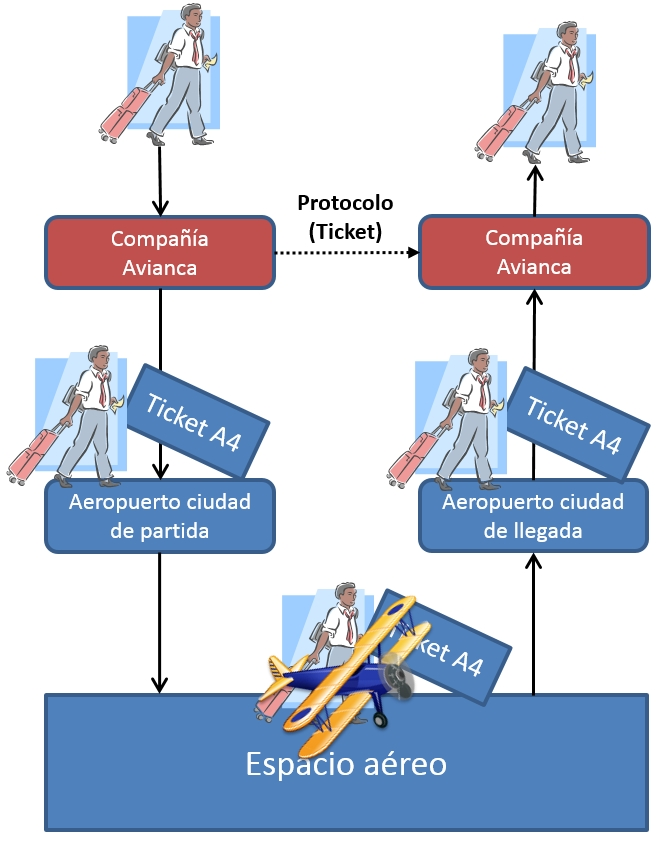
\includegraphics[scale=0.4]{Imagenes/modelo_aviacion_red}
	\label{fig:modelo_aviacion_red}
\end{figure}

En fin de cuentas, todo sistema de comunicación comienza por la conquista de un recurso para la comunicación. En las telecomunicaciones, los recursos más usados son las líneas de cobre, la fibra óptica, el espectro radioléctrico (ERE) y la luz, como es el caso de los sistemas de comunicaciones conocidos como Free Space Optics. Pero nada nos limita a pensar en otras posibilidades como el uso del ultrasonido e incluso no sería descabellado llegar descubrir información que viaja sobre las ondas gravitacionales que se desplazan por el universo.\\

En la Figura \ref{fig:CapasV1} se tiene un modelo de capas para el caso en que se usa el ERE. \\

%\vspace{200px}
\begin{figure}[h!]
	\captionsetup{justification = raggedright, singlelinecheck = false}
	\caption{Modelo de capas para un sistema de comunicaciones inalámbricas en red} 
	\centering
	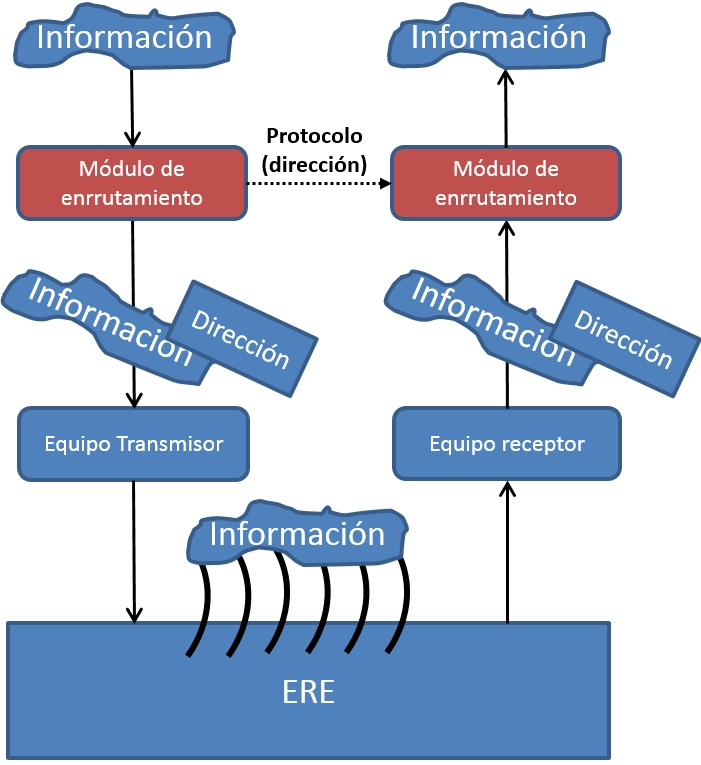
\includegraphics[scale=0.6]{Imagenes/CapasV1}
	\label{fig:CapasV1}
	%		\captionsetup{justification=raggedright,font={scriptsize,bf,it}}
	%		\caption*{fuente: http://superkuh.com/rtlsdr.html}
\end{figure}

Algunos conceptos importantes para este modelo son:   

\begin{itemize}
	\item  \textbf{Las ondas electromagnéticas:} Son el vehículo que hace uso del ERE para conducir información mediante la modulación de uno de sus parámetros. Claro está que en las radio comunicaciones solo se usan las ondas electromagnéticas que se encuentran en una banda del espectro conocida como el espectro radio eléctrico. Se trata de la banda comprendida entre 30 kHz y 300 GHz.
    \item  \textbf{ La modulación:} Consiste en el proceso de montar la información sobre algún medio de comunicación. En el caso de las radio comunicaciones, la información puede montarse sobre la onda en forma forma de variaciones de la amplitud de la onda, como cuando una persona usa su linterna, en cuna cueva para enviar mensajes a un compañero variando la intensidad de la luz. Pero también es posible hacer que la información viaje en forma de variaciones de la frecuencia o de la fase de la onda. 
    \item  \textbf{La Modulación de amplitud (AM):} Se da cuando la información viaja sobre una portadora en forma de variaciones de amplitud.
    \item  \textbf{Modulación de Frecuencia (FM):} Es el nombre que toma el método de modulación que usa la frecuencia de la onda portadora para llevar información.
    \item  \textbf{Modulación de Fase (PM):} Es el tercer método de modulación de una onda portadora y consiste en la posibilidad de hacer que la información viaje en forma de variaciones de la fase de la onda portadora.
\end{itemize}

Como en el caso del transporte aéreo, se ha introducido un módulo de enrrutamiento para que el modelo corresponda al de un sistema de comunicaciones en red. Algunos elementos de un modelo de capas son los siguientes:

\begin{itemize}
	\item  \textbf{Entidades pares:} En cada capa se tiene un módulo en el transmisor que hace pareja con un módulo en el receptor, esto es lo que se conoce como entidades pares.
    \item  \textbf{Protocolo:} corresponde a todo aquello que pueda ser usado entre las entidades pares para entenderse mutuamente. Por ejemplo, el módulo de enrrutamiento en la parte transmisora puede agregar a la información una etiqueta con la dirección de destino. El mismo módulo en en receptor leer esa dirección, para poder tomar una decisión que puede ser la de extraer la información para entregarla o la de encaminar esa información hacia otro destino.
    \item  \textbf{Canal:} se refiere aquello que se usa como medio para que viaje la información desde un origen hasta un destino. Es justo aquello que plantea los principales retos a un sistema de comunicaciones. Cada caso particular puede tener su propio canal. Así, en las radiocomunicaciones punto a punto el canal está usualmente representado por una banda concreta del ERE, pero limitada al espacio geográfico y al duración que corresponda según las normas para el sistema de comunicaciones dado. El canal inalámbrico representa enormes retos para los sistemas de comunicaciones pues el proceso de transmisión y recepción no solo deben sortear la necesidad de emitir y recibir ondas de radio sino la de considerar los diferentes fenómenos que esas ondas pueden sufrir en su propagación. 
\end{itemize}

La Figura \ref{fig:ModeloRadiodifusion} muestra el modelo de capas que podría ser usado para explicar el funcionamiento de la radio difusión. \\

\vspace{300px}
\begin{figure}[h!]
	\captionsetup{justification = raggedright, singlelinecheck = false}
	\caption{Modelo de capas para la radio difusión} 
	\centering
	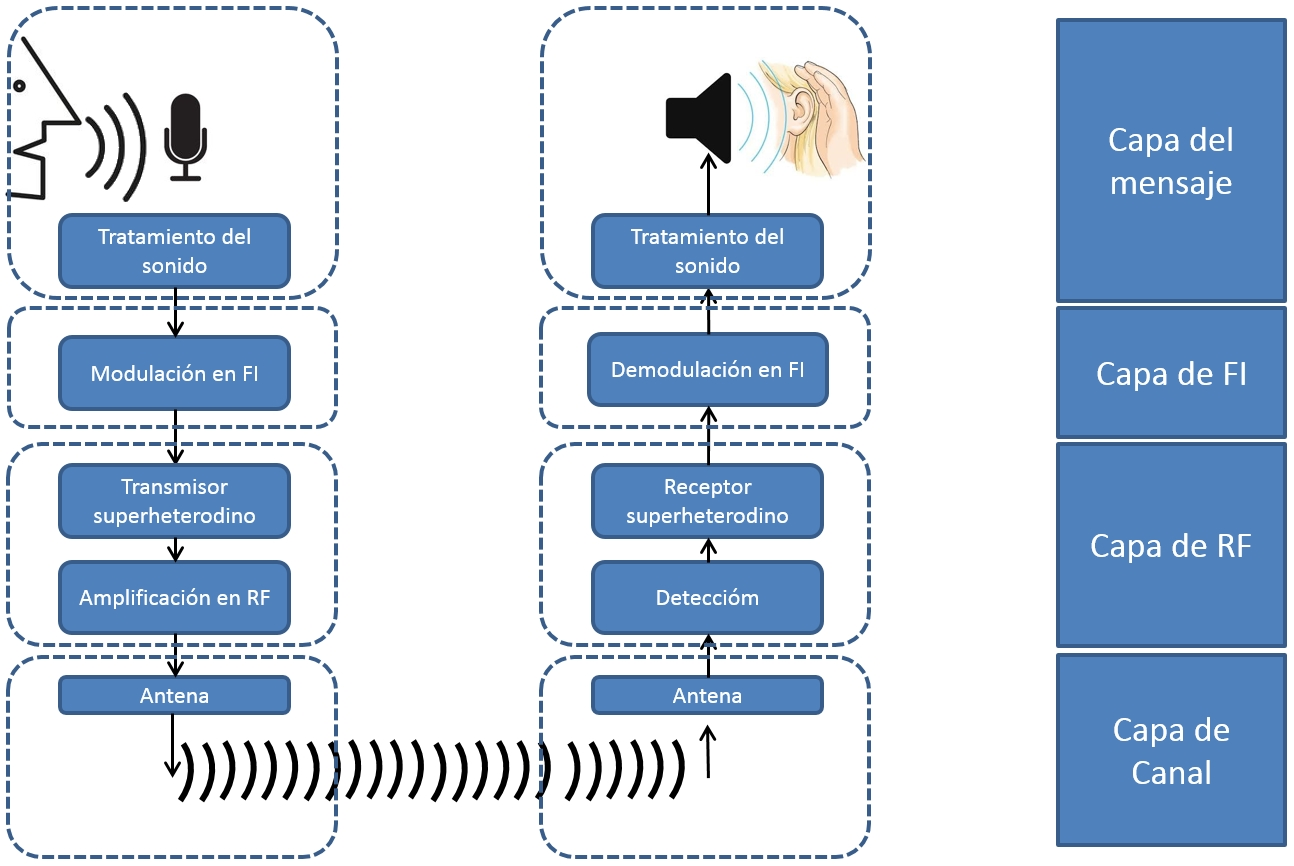
\includegraphics[scale=0.4]{Imagenes/ModeloRadiodifusion}
	\label{fig:ModeloRadiodifusion}
\end{figure}


A diferencia de las comunicaciones punto a punto, en un sistema de radiodifusión se tiene una radio base que emite una señal para que sea sintonizada por cientos o miles de receptores, como es el caso de lo que se conocen como emisoras de radio y de televisión. Como podemos ver, se usan conceptos ya vistos. Las dos capas superiores corresponden al estudio (las oficinas) de una emisora, donde están los equipos que capturan el mensaje de la mejor manera posible, pero también el equipo que realiza la modulación de una señal portadora de frecuencia intermedia que es común para cualquier equipo similar. Por ejemplo, para la radiodifusión AM se ha establecido un valor de frecuencia intermedia igual a 455kHz, mientras que en la de FM es de 10.5 MHz. Las razones para usar una frecuencia intermedia (FI) son las siguientes: \\

\begin{itemize}
	\item  Facilita la separación entre dos tipos de equipos, los que funcionan con baja potencia y baja frecuencia, que pueden usarse en las premisas de la emisora sin temor a causar daños a la salud y los de alta potencia y altas frecuencias, pensados para lograr alcanzar las coberturas necesarias y en las frecuencias necesarias, que deben ser ubicados bajo cuidados especiales, por ejemplo en una torre de comunicación.
    \item  El transmisor superheterodino representa una solución para traducir la señal modulada con FI a una señal modulada con la frecuencia RF. En términos espectrales, consiste en desplazar el espectro de la señal modulada con FI para que quede centrado en la frecuencia $f_c$ como denotaremos en adelante la frecuencia de la portadora o frecuencia RF.
    \item  Igualmente, el receptor superheterodino representa el paso de la señal modulada en la frecuencia RF a la FI
	\item  Gracias a que los valores de FI son estandarizados, es posible combinar el uso de  equipos de diferentes fabricantes para implementar una emisora de radiodifusión.
    \item  Los dispositivos electrónicos usados en cualquiera de las dos etapas se pueden producir a escala a precios bajos ya que tienen funciones limitadas.
\end{itemize}

En la práctica, el modelo de capas de un sistema de radiodifusión puede ser algo más complejo ya que el estudio se localiza usualmente en un lugar poblado, como una ciudad, mientras que los equipos de transmisión, organizados en una radio base, se ubican usualmente en una montaña desde la cual es posible emitir una señal con suficiente potencia para cubrir un gran zona geográfica. Eso significa la necesidad de introducir un sistema adicional de comunicación punto a punto para comunicar el estudio con la radio base. Por ahora no resulta conveniente entrar a revisar un modelo de capas para este caso.\\


%%%%%%%%%%%%%%%%%%%%%%%%%%%%%%%%%%%%%%%%%%%%%%%%%%%%


\chapter{Simulación de señales y sistemas con GNU Radio}

Este capítulo tiene el fin de estudiar lo que significa Software Defined Radio (SDR) y un tipo de hardware usado en SDR. Con el fin de lograr que el estudiante tenga contacto con un hardware real, hemos seleccionado el USRP-2920 de la empresa National Instruments, pero también se busca generalizar el conocimiento sobre ese hardware en forma de modelos más generales que le brinde al estudiante la capacidad de descubrir y comprender cualquiera de los tipos de hardware existentes. El mayor énfasis se hace en que estudiante conozca lo que un hardware SDR representa. \\

\section{Herramientas que compiten con GNU Radio}
La simulación de señales y sistemas es una estrategia que se viene usando desde la aparición del computador. Se ha usado para poner a prueba diversos métodos digitales antes de pensar en su implementación en sistemas reales. La diferencia con el estado del arte de hoy es que lo que está plasmado en una simulación puede pasar a ser parte del mundo real tan pronto como el programador lo desee, siempre y cuando en la simulación se respeten parámetros que limitan el mundo real. Pero muchas veces la simulación es realizada con otros propósitos. Supongamos que deseamos descubrir un método para corregir el efecto Doppler que se produce entre un radio transmisor y un radio receptor, es decir, en un canal inalámbrico. Para probar ese método resulta útil poder simular un canal que no tenga otro efecto de propagación que el Efecto Doppler.\\ 

Cualquier lenguaje de programación puede ser usado en simulación y también como parte de un sistema real de comunicaciones basada en SDR, pero algunas entidades han llevado más allá a ciertos lenguajes y herramientas, entre los cuales tenemos los siguientes:

\subsection{Matlab y Simulink}
Lo destacable es lo siguiente:
\begin{itemize}
   \item [$\bullet$] Es una plataforma de programación y a la vez un lenguaje de programación que solo corre sobre esa plataforma.
	\item [$\bullet$] Tiene una larga tradición en simulación, lo que le ha permitido contar con librerías muy maduras y es muy usada por los científicos.
    \item [$\bullet$] Requiere contar con licencia de Matlab y de las librerías que se vayan a usar.
    \item [$\bullet$] Las soluciones resultan siendo dependientes de Matlab. Es decir, si un usuario interesado en una solución no cuenta con Matlab, no podrá usarla.
    \item [$\bullet$] Puede soportar un amplio rango de equipos SDR.
    \item [$\bullet$] Las soluciones son pesadas desde el punto de vista de computo debido a la necesidad de correr sobre Matlab.
    \item [$\bullet$] Simulink facilita la programación gráfica, es decir, evita en gran manera la escritura de código.
\end{itemize}

\subsection{LabView de National Instruments}
Lo destacable
\begin{itemize}
	\item [$\bullet$] Es un ambiente de programación gráfica de National Instruments (NI) que también puede producir código en c++.
    \item [$\bullet$] Tiene bastante aceptación en la industria.
    \item [$\bullet$] En lo demás, tiene las mismas cualidades que MATLAB con simulink.
\end{itemize}
\subsection{System Vue de KeySight}
\begin{itemize}
	\item [$\bullet$]  Es un ambiente de programación gráfica de KeySight que puede aceptar varios lenguajes de programación.
    \item [$\bullet$] Está muy orientada a la industria.
    \item [$\bullet$]  Las licencias son muy costosas, solo al alcance de la industria, aunque se tiene en algunos laboratorios de investigación de las universidades.
\end{itemize}

%%%%%%%%%%%%%%%%%%%%%%%%%%%%%%%%%%%%%%%%%%%%%%%%

\section{GNU Radio como plataforma de simulación y de desarrollo}

GNU Radio es una de las opciones más importantes para llevar a la práctica las soluciones basadas en SDR. Por lo menos es la opción más usada a nivel de investigación. La empresa National Instruments también ha complementado su plataforma de software de LabView para que sea usada como una herramienta de software para GNU Radio. Matlab e incluso Simulink de Matlab son también complementos para soportar diversos tipos de hardware, como es el caso de los USRP. En principio, cualquier lenguaje de programación puede servir para producir la componente de software en SDR, pero la mayoría de investigadores se inclinan por C++ y Python, por tener librerías que crecen muy dinámicamente con un acompañamiento internacional. Precisamente esas librerías están en GNU Radio. De hecho, las librerías que tiene el lenguaje Python son heredadas de las que tiene C++.\\

\textbf{Modelo que relaciona software y hardware}
El siguiente modelo, deja claro lo que se espera de GNU Radio y del hardware que se puede llegar a complementarlo. \\

%\setcounter{figure}{33}
\vspace{400px}
\begin{figure}[h!]
	\captionsetup{justification = raggedright, singlelinecheck = false}
	\caption{Modelo SDR que relaciona GNU Radio con el Hardware.} 
	\centering
	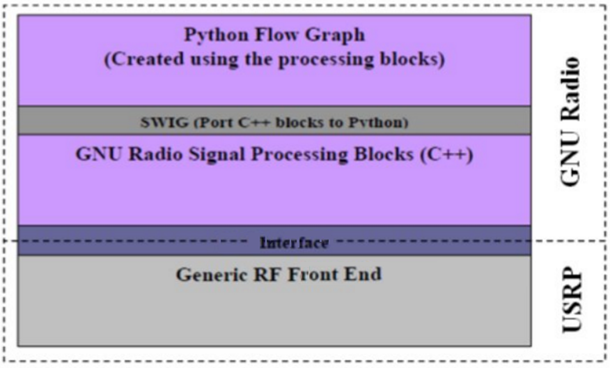
\includegraphics[scale=0.7]{Imagenes/Modelo-SDR.png}
	\label{fig:Modelo-SDR}
		\captionsetup{justification=raggedright,font={scriptsize,bf,it}}
		\caption*{fuente:  El gráfico ha sido adaptado de trabajo: Experimental Study of OFDM Implementation Utilizing GNU Radio and USRP – SDR. Proceedings of the 2009 IEEE 9th Malaysia International Conference on Communications. Kuala Lumpur Malaysia. 15 -17 Diciembre, 2009.
		}
\end{figure}

De este modelo, se puede deducir lo siguiente: \\

\begin{itemize}
	\item [$\bullet$]GNU Radio está compuesto de dos capas que cooperan:	
	\begin{itemize}
		\item [$\bullet$] GNU Radio Signal Processing Blocks (C++). Es una librería en C++ que contiene todos los desarrollos comunes a ser utilizados en programación en el lenguaje C++.
		\item [$\bullet$] Python Flow Graph. Consiste en un desarrollo hecho para facilitar la programación lenguaje en Python o también la basada en un lenguaje gráfico o Flujogramas.
	\end{itemize}
	\item [$\bullet$] Cuando se programa usando Flujogramas, estos producen el código en Python, usando una librería de GNU Radio en Python. Pero esa librería es importada de C++, de modo que indirectamente se usa la librería GNU Radio de C++. La capa señalada com SWIG es la encargada de realizar la importación de C++ de modo que el desarrollador de Python tenga la sensación de que su trabajo es completamente basado en Python.
	\item [$\bullet$] Desde el punto de vista teórico, la componente de software que se desarrolla, se conecta directamente con el hardware, el cual aparece señalado en la figura anterior como USRP, pero que en términos más genéricos, puede llamarse Front End Genérico de RF. Pero en la práctica se requiere algo más: el hardware está alojado en un computador, el cual puede ser tan grande o tan pequeño como sea posible o incluso estar embebido en el hardware, pero este hecho hace que en la práctica se tenga en realidad dos elementos por conectar: el computador y el hardware que para nuestro ejemplo es un USRP. Por esa razón, se requiere introducir un medio de comunicación para estos dos elementos. Ese medio usualmente está representado en los puertos de comunicación que estos dos elementos tengan como: USB, Ethernet u otros.  En la actualidad, los equipos USRP optan por la opción de puerto Gigabit Ethernet, pero otros tipos de hardware como Realtek RTL2832U, optan por puerto USB. En todo caso, cuando hay un medio de comunicación de por medio, surge la necesidad de desarrollar una capa sobre este medio que se encarga de adaptar la información a este medio. En otras palabras, se requiere un software que llamaremos driver, el cual toma la información que entrega el software de la solución SDR, y la traduce para que pueda viajar por el  protocolo de comunicación. Del lado del Front End se requiere también un driver similar para que la comunicación se dé. Para el caso de los USRP ese driver es conocido com UHD (USRP Hardware Driver)
\end{itemize}



\begin{itemize}
	\item [$\bullet$] GNU Radio es realmente una librería de radiocomunicaciones para lenguaje C++, con una versión en el lenguaje Python. El GRC es un ambiente de programación gráfica que aprovecha esa librería y produce código en Python o en c++.
    \item [$\bullet$] Es de uso libre.
    \item [$\bullet$] Las aplicaciones hechas con gnuradio son muy livianas y pueden llevarse a producción sin que dependan de una plataforma determinada.
     \item [$\bullet$] Es ampliamente usada por científicos y académicos.
\end{itemize}

%%%%%%%%%%%%%%%%%%%%%%%%%%%%%%%%%%%%%%%%%%%%%%%%%%%%

\section{Simulación de señales bandabase}

Podría decirse que la Radio Definida por Software representa el uso de la la teoría de señales y sistemas discretos llevada a la práctica. La aplicación práctica implica una relación entre el mundo físico que es por naturaleza continuo y el uso de técnicas de computación que es por naturaleza discreto.\\

Para entenderlo mejor, vamos a volver al sistema de radiodifusión expresado en el modelo de capas de la Figura \ref{fig:ModeloRadiodifusion}. Un sistema de radiodifusión es por su origen analógico tanto por la naturaleza del mensaje como de los equipos usados y la señal emitida. Sin embargo, con los avances tecnológicos, las soluciones que hoy se tienen en el mercado combina tecnología digital y analógica, ya que no tiene lógica alguna usar hoy tecnología analógica para crear un sistema de comunicación por el solo hecho de que ese sistema es analógico. Es por esa razón que cuando hacemos una visita a los estudios de una emisora AM o FM encontramos que todos los equipos nuevos son digitales, aunque AM y FM son modulaciones analógicas.\\
Para entenderlo mejor, en la Figura \ref{fig:ModeloRadiodifusionSDR} se presenta un modelo de capas para un  sistema de radio difusión analógico implementado con tecnología digital, que en realidad es una combinación de tecnologías analógicas y digitales. La combinación se realiza de la siguiente manera:

%\setcounter{figure}{0}
%\vspace{200px}
\begin{figure}[h!]
	\captionsetup{justification = raggedright, singlelinecheck = false}
	\caption{Modelo de capas de un sistema de radio difusión analógico implementado con tecnología digital} 
	\centering
	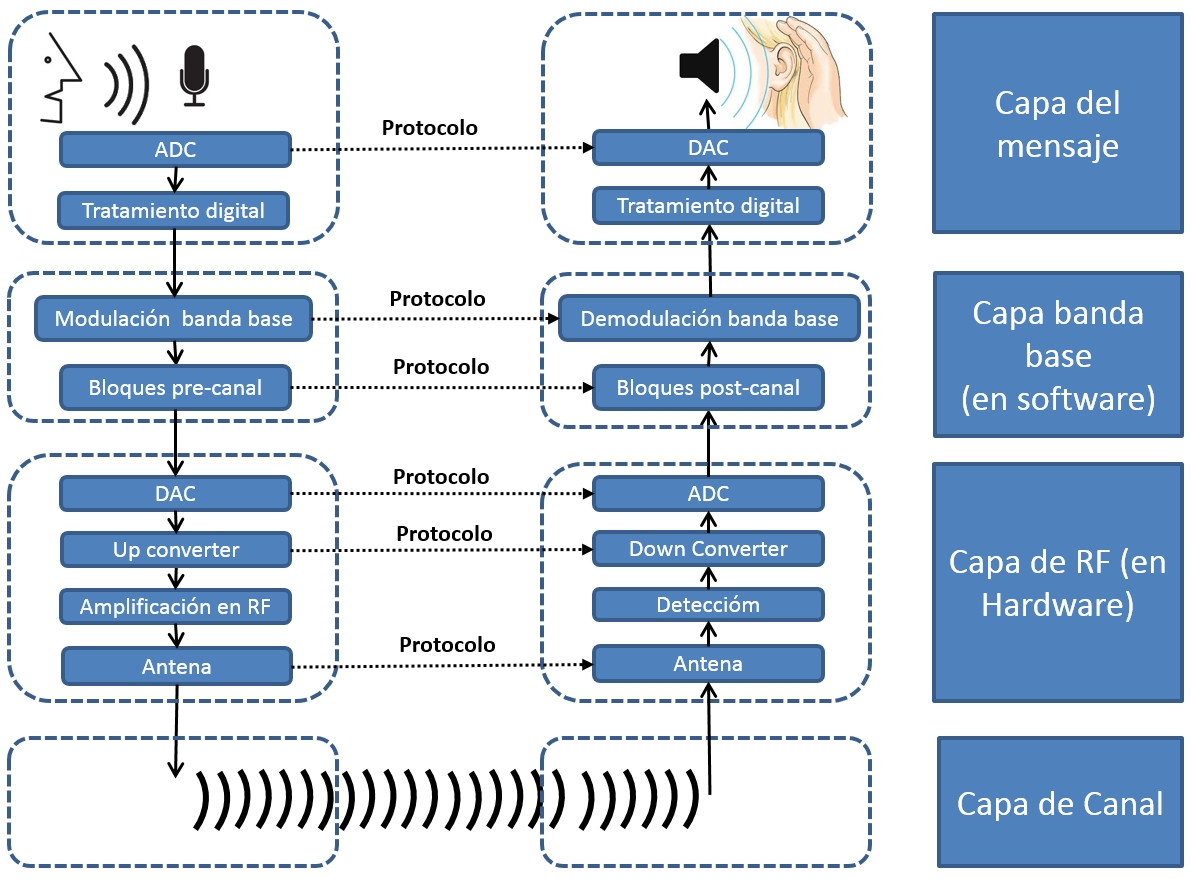
\includegraphics[scale=0.45]{Imagenes/ModeloRadiodifusionSDR}
	\label{fig:ModeloRadiodifusionSDR}
\end{figure}

\begin{itemize}
	\item [$\bullet$] Se conserva la naturaleza analógica del mensaje y de la señal emitida.
    \item [$\bullet$] Tan pronto se tiene la señal del mensaje, se traduce a datos mediante un conversor Análogo Digital (ADC). Este proceso implica el uso de algunos conceptos como el Teorema de Nyquist para realizar un muestreo adecuado a la señal; la cuantificación; la codificación PCM (del inglés Pulse Code Modulation).
    \item [$\bullet$] Lo que sigue es el uso de métodos numéricos que se implementan en un equipo de cómputo tanto para realizar un tratamiento digital del sonido del mensaje pero también, realizar la modulación. 
    \item [$\bullet$] En lugar de usar frecuencias intermedias, la modulación se realiza en banda base, que equivale a obtener una señal que tenga el mismo espectro de la señal modulada tradicionalmente, pero ahora, centrado en la frecuencia cero. 
    \item [$\bullet$] Lo anterior implica nuevos retos teóricos y técnicos, pues la señal modulada en banda base resulta ser compleja y se conoce como la Envolvente Compleja
    \item [$\bullet$] El reto teórico consiste en la necesidad de saber modular y demodular señales usando el concepto de Envolvente Compleja
    \item [$\bullet$] El reto técnico aparece con la capa que hemos llamado Capa RF, donde predominan tareas con equipo analógico analógicas. Antes de entregar la señal a esta capa es necesario preparar la señal para su paso a un medio analógico, eso es lo que hemos llamado Bloques Pre-canal. Luego, la señal pasa al dominio continuo usando un Conversos Digial Análogo (DAC).
    \item [$\bullet$] El Up converter es un circuito que permite mover el espectro de la señal recibida para que quede centrado en la frecuencia RF.
    \item [$\bullet$] La antena simplemente traduce la señal eléctrica en señal obtenida en señal electromagnética
    \item [$\bullet$] Es claro que en la parte receptora se tienen componentes que hacen pareja con los mencionados anteriormente, para recibir la señal, desplazar el espectro de esa señal a la frecuencia cero, usando un Down Converter y así sucesivamente.\\

Este modelo deja precisamente claro la tendencia natural para la implementación de los futuros sistemas de comunicaciones basados en Software Defined Radio (SDR). Básicamente, un sistema de SDR tiene las siguientes características:

    \item [$\bullet$] Tienen una componente de software y una de hardware
    \item [$\bullet$] En la componente de hardware se realiza unas tareas que son comunes para cualquier sistema de comunicaciones: mover la señal en el dominio de las frecuencias para centrarla en la frecuencia RF, amplificarla de acuerdo a las necesidades, transmitirla en forma de ondas de radio. En fin, la componente de hardware corresponde a la Capa RF en la Figura \ref{fig:ModeloRadiodifusionSDR}. Las prácticas propuestas en este libro se apoyan mayormente en un hardware SDR de National instruments conocido como USRP.
    \item [$\bullet$] La componente de software se aloja en un computador y es allí donde se implementan soluciones para sistemas específicos de comunicaciones. A diferencia de lo que ocurre en los sistemas analóticos, los métodos que aquí se implementan son muy cercanos a los teóricos, por ejemplo, una modulación FM puede estar dada por una o varias fórmulas o por uno o más algoritmos. 
    \item [$\bullet$] En la componente de software la programación se realiza para señales banda base, para lo cual existen diversas herramientas de programación. La que usaremos en el presente libro se conoce como gnuradio. Se trata principlamente de una librería que reune las experiencias en el tema de una gran comunidad de desarrolladores
    \item [$\bullet$] Al lado de gnuradio, también se cuenta con una herramienta conocida como GRC, que permite realizar la programación gráfica, usando bloques, de manera similar a lo que se puede lograr usando Simulink de Matlab. De hecho, Simulink de Matlab también puede ser usada para implementar soluciones SDR.
\end{itemize}

\subsection{La Conversión Análogo Digital}
Como se vió anteriormente, en la parte transmisora se requiere usar un dispositivo ADC y en la receptora un dispositivo DAC. Puede decirse que estos elementos sirven de compuerta entre el mundo continuo y el digital. Conocer muy las capacidades y las limitaciones que tienen estos dispositivos es clave para poder lograr un montaje funcional. A continuación se revisan los principales procesos y características de un ADC:

\subsubsection{El muestreo. La frecuencia de muestreo y el ancho de banda}

El ADC puede ser visto como un medidor de la tensión de una señal, que mide en tiempos discretos separados entre sí en un tiempo $T_s$. Por lo tanto, las mediciones se presentan a la frecuencia de muestreo $F_s=\frac{1}{T_s}$.\\

Los siguientes son los aspectos que merecen mayor atención: \\
\begin{itemize}
	\item [$\bullet$] De acuerdo al Teorema de Nyquist, la señal muestreada puede llegar a tener una frecuencia máxima igual a $F_{max}=\frac{F_s}{2}$ se tiene el principal parámetro. Eso significa que un un ADC está limitado en ancho de banda.
    \item [$\bullet$] El costo en dinero que puede tener un ADC se eleva exponencialmente con la frecuencia de muestreo que soporte.
    \item [$\bullet$]  El muestreo es un proceso reversible, al menos desde el punto de vista teórico siempre y cuando la señal haya sido muestreada respetando el Teorema de Nyquist. \\
    
La puesta en práctica del Teorema de Nyquist es lo que produjo en los año 60 la revolución PCM, que es cuando la telefonía, siendo la red más grande del mundo adoptó la tecnología PCM en toda su dimensión. La idea consistía en tomar la señal de voz de un teléfono, limitar su ancho de banda hasta 4 kHz, muestrearla a una frecuencia de muestreo de 8 kHz, con lo cual el periodo de muestreo o distancia de muestra y muestra sería de $125 \mu seg$ . Esa distancia de tiempo entre muestra y muestra se aprovechó para enviar allí muchas más señales de voz también muestreadas. Se elevó entonces la capacidad de las redes, pues ya no era necesario tener un par de hilos de cobre entre dos puntos para conducir cada llamada teléfonica, pues muchas llamadas telefónicas podían ahora viajar sobre un mismo par de hilos de cobre.\\

Usualmente los estudiantes no se convencen del mensaje que envía el Teorema de Nyquist y que puede enunciarse así: si tu muestreas una señal usando una frecuencia de muestre que sea igual o superior a dos veces la frecuencia máxima que esa señal pueda llegar a tener, siempre podrás recuperar, sin pérdida alguna, la forma continua de esa señal a partir de la versión discreta. Ósea que el proceso de muestreo para de dejar de transmitir la señal todo el tiempo y hacerlo solo por instantes, no implica que la señal continua haya dejado de existir. \\

    
\end{itemize}
\subsubsection{La cuantificación. El Diapasón de cuantifiación}
En un ADC La cuantificación es inseparable del proceso de muestreo. Surge debido a que un ADC nunca puede llegar a entregar una señal muestreada como la que teóricamente esperamos. Esto es debido a las siguientes posibles razones:
\begin{itemize}
	\item [$\bullet$] La salida del ADC es un número acotado en bits. Algunos pueden permitir una configuración, por ejemplo para usar 32 bits/muestra o 64 bits/muestra. Los usados en telefonía fija deben cumplir una recomendación de la UIT-T que establece que son 8 bits/muestra 
    \item [$\bullet$]Por lo anterior, el proceso de cuantificación equivale a una una especie de muestreo en amplitud. Pero la cuantificación no es un proceso reversible como sí lo es el muestreo cuando se cumple el Teorema de Nyquist. \\
    
En la Figura \ref{fig:3_bit_cuantizacion} se presenta una comparación entre una señal continua y su versión cuantificada a la razón de 3 bits/muestra.

\begin{figure}[h!]
	\captionsetup{justification = raggedright, singlelinecheck = false}
	\caption{Comparación entre una señal continua y una cuantificada a la razón de 3 bits/muestra} 
	\centering
	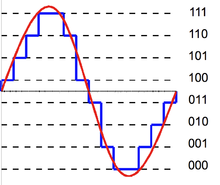
\includegraphics[scale=1]{Imagenes/3-bit_cuantizacion}
	\label{fig:3_bit_cuantizacion}
\end{figure}
    \item [$\bullet$]Por lo anterior, un ADC tiene unos límites inferior y superior para la amplitud de la señal que puede entregar
    \item [$\bullet$]Pero algo no menos relevante es que un ADC también tiene unos límites inferior y superior para la señal que recibe. La diferencia entre esos dos limites es lo que se conoce como Diapasón de cuantificación.
    \item [$\bullet$]Los siguientes son los problemas más comunes con el uso de ADC:
    \begin{itemize}
		\item [$\bullet$] La señal que entra al ADC puede ser tan débil que la cuantificación la deforma completamente porque queda expresadas con muy pocos niveles de amplitud.
        \item [$\bullet$] La señal que entra al ADC puede ser tan fuerte que se sale del diapason que soporta, de modo que las amplitudes que se salen del diapasón desaparecen deformando la señal.
        \item [$\bullet$] La señal entrante puede tener un ancho de banda que supera el soportado por el ADC, lo cual hace que la señal resulte irrecuperable.
    	\item [$\bullet$]\textcolor{Red}{El resultado de la ...}
	\end{itemize}
      
\end{itemize}

\subsection{El paso a un código de línea. PCM}

\subsection{La Conversión Digital Análoga}
La Conversión Digital Análoga es el proceso inverso de la Conversión Análoga Digital. En este sentido, el DAC tiene parámetros similares al ADC.

\subsection{Filtros digitales}
\textcolor{Red}{[falta]. }\\

La idea es explicar lo que significan los filtros digitales. Básicamente como un sistema LIT con una respuesta al impulso

\subsection{interpoladores}
\textcolor{Red}{[falta]}
\subsection{Decimadores}
\textcolor{Red}{[falta]}

\subsection{Transformada Rápida de Fourier (FFT)}
Se trata de un algoritmo que permite calcular, con un óptimo recurso computacional, la siguiente fórmula.

\begin{equation} \label{capdos}
	 C_{k} =  \sum_{n=0}^{N-1}x_{N} [n]e^{-j2 \pi kn/N}
\end{equation}

\subsubsection{Aspectos relevantes de aplicación práctica:}
El uso de la FFT en la práctica pasa por las siguientes consideraciones:
\begin{itemize}
	\item  [$\bullet$] La FFT puede servir para obtener la RSF de una señal de la siguiente manera:
	\begin{itemize}
		\item [$\bullet$]  Si x[n] proviene de una señal continua, el muestreo debe haber sido realizado respetando el Teorema de Nyquist.
		\item [$\bullet$]  La señal debe ser periódica en N.
		\item [$\bullet$]  La FFT se aplica una única vez, para N, con lo cual se produce un espectro estático.
		\item [$\bullet$]  El espectro obtenido debe ser dividido en N.
	\end{itemize}
	\item [$\bullet$] La FFT puede servir para obtener una aproximación de la TF de una señal de la siguiente manera:
	\begin{itemize}
	\item [$\bullet$]  Si x[n] proviene de una señal continua, el muestreo debe haber sido realizado respetando el Teorema de Nyquist. 
	\item [$\bullet$]  Ente más grande sea N, la aproximación será mejor. Es claro que si N es exageradamente grande, resulta engorroso tener que esperar mucho tiempo para obtener el resultado, además la resolución que se obtiene puede ser exagerada para nuestras necesidades reales.
	\end{itemize}

	\item [$\bullet$]  La FFT puede servir para obtener un espectro dinámico o instantáneo de una señal de la siguiente manera
		\begin{itemize}
	\item [$\bullet$]  Con las muestras de x[n] se van creando paquetes de N muestras. N no debe ser tan grande, se recomienda que sea igual al número de puntos que su ojo podría distinguir en la pantalla de su computador, por ejemplo N=1024 o N=512
	\item [$\bullet$]  Se aplica la FFT a un paquete de N muestras para obtener N muestras espectrales. Luego se obtiene la magnitud al cuadrado y se convierte a dB 
	\item [$\bullet$]  Se repite lo anterior para cada uno de los subsiguientes paquetes, con lo cual en la pantalla veremos un espectro que va variando en el tiempo.
		\end{itemize}
	\item [$\bullet$]  La FFT puede servir para obtener la PSD si se aplica de la siguiente manera:
		\begin{itemize}
		\item [$\bullet$]  Se hace lo mismo que el caso anterior, pero cada paquete de N muestras espectrales se va promediando con los anteriormente recibidos.
		\end{itemize}
\end{itemize}
\subsection{La IFFT}
Representa el mecanismo inverso a la FFT. Por lo tanto se apoya en la ejecución de la siguiente fórmula:\\

\begin{equation} \label{capdos_uno}
	 x_{N}[n] =  \sum_{k=0}^{N-1}C_{k}e^{j2 \pi kn/N}
\end{equation}
%\vspace{30px}

\subsection{Simulación de un analizador de espectros}

Analizaremos dos bloque que tiene GNU Radio y que usan la FFT: El bloque FFT y el bloque QT GUI Frequency Sink. En la figura \ref{fig:la-FFT} 

\begin{figure}[h!]
	\captionsetup{justification = raggedright, singlelinecheck = false}
	\caption{Flujograma La-FFT.grc. Comparación del bloque FFT con QT GUI Frequency Sink para observar la PSD de una señal binaria bipolar aleatoria.} 
	\centering
	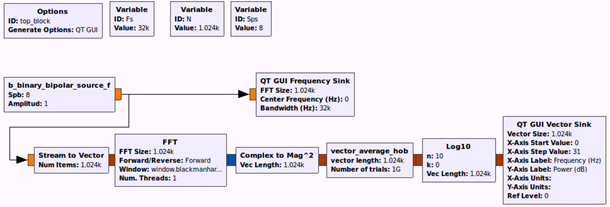
\includegraphics[scale=1]{Imagenes/La-FFT.png}
	\label{fig:la-FFT}
	%		\captionsetup{justification=raggedright,font={scriptsize,bf,it}}
	%		\caption*{fuente: http://superkuh.com/rtlsdr.html}
\end{figure}

La siguiente figura presenta el resultado del bloque QT GUI Frequency Sink

%\vspace{100px}
\begin{figure}[h!]
	\captionsetup{justification = raggedright, singlelinecheck = false}
	\caption{PSD obtenida usando QT Frequency Sink.} 
	\centering
	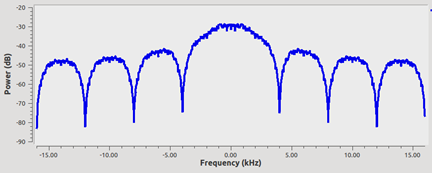
\includegraphics[scale=1]{Imagenes/PSD-QT.png}
	\label{fig:la-PSD-QT}
	%		\captionsetup{justification=raggedright,font={scriptsize,bf,it}}
	%		\caption*{fuente: http://superkuh.com/rtlsdr.html}
\end{figure}

La figura \ref{fig:la-PSD-FFT} presenta el resultado del bloque FFT.

\vspace{200px}
\begin{figure}[h!]
	\captionsetup{justification = raggedright, singlelinecheck = false}
	\caption{PSD obtenida usando el bloque FFT combinado con otros bloque} 
	\centering
	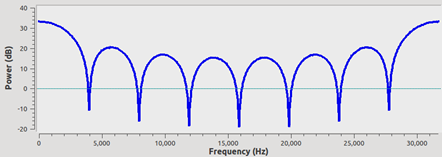
\includegraphics[scale=1]{Imagenes/PSD-FFT.png}
	\label{fig:la-PSD-FFT}
	%		\captionsetup{justification=raggedright,font={scriptsize,bf,it}}
	%		\caption*{fuente: http://superkuh.com/rtlsdr.html}
\end{figure}

Conclusiones de las observaciones y recomendaciones para usar estos bloques:

\begin{itemize}
	\item [$\bullet$]  Obtener la PSD usando el bloque FFT requiere preparar el vector, pasar el resultado de la FFT a magnitud al cuadrado, realizar un promediado con los vectores previos, convertir a dB y graficar. 
	\item [$\bullet$]  Aunque parezca diferente, la imágen obtenida con el bloque FFT es equivalente a la del bloque QT GUI Frequency Sink, ya que la teoría de Fourier dice que la Transformada de Fourier Discreta (DFT) es periódica en $F_{r}= 2\pi Rad/seg$ y eso significa que es periódico en la frecuencia de muestreo $F_{s}$ (Hz)de la señal vista en el tiempo. Por eso, si el bloque FFT pudiese ser configurado para que muestre el espectro entre $\dfrac{-F_{s}}{2}$ y $\dfrac{F_{s}}{2}$ tendríamos imágenes similares. La imágen obtenida con el bloque FFT es más continua debido a que el bloque vector-average-hob, usado como complemento al bloque FFT realiza un promediado más prolongado.
	\item  [$\bullet$] La frecuencia máxima que puede mostrar un Analizador de Espectros es igual a la frecuencia de muestreo sobre 2. También puede observarse que el ancho de banda B, que abarca tanto frecuencias negativas como positivas, es igual a la frecuencia de muestreo.
	\item [$\bullet$]  N es el tamaño del vector y es igual al orden de la FFT, también es igual al número de puntos que son graficados en la ventana. De deduce que la resolución espectral es 	$ f_{Resol} = \dfrac{frecuencia de muestreo}{N}$
	\item [$\bullet$]  Finalmente, es importante tener en cuenta que la PSD se calcula usualmente a señales que son parte del mundo continuo, por ejemplo la señal que se emite desde un transmisor, la que se recibe en un receptor, la que produce un micrófono o la que usa una bocina. Desde este punto de vista, no es usual buscar la PSD de señales que pueden encontrarse en bloques intermedios como por ejemplo un codificador o un modulador digital bandabase.	
\end{itemize}

%%%%%%%%%%%%%%%%%%%%%%%%%%%%%%%%%%%%%%%%%%%%%%%%%

\section{Simulación de señales paso bandas}



\subsection{La Modulación AM}

\textcolor{red}{[Falta: Oscar Reyes]} %\OR a nivel de flujograma??

\subsection{La Modulación FM}

\textcolor{red}{[Falta: Oscar Reyes]}


\subsection{El heterodinado}
\textcolor{red}{[Falta: Oscar Reyes]}

\subsection{Conversión RF}

La Conversión RF es un término que se está introduciendo en este libro, por lo tanto, no lo encontrará en ninguna otra fuente anterior a esta. Se refiere al proceso de pasar una señal real de su correspondiente Envolvente Compleja (EC) y viceversa. La razón para introducir este concepto es meramente pedagógica y consiste en lo siguiente: cuando un ingeniero trabaja con GNU Radio, estará operando casi siempre con la EC, mientras la señal que viaja entre las antenas es pasobandas. La forma en que se define a continuación la Conversión RF ayuda a que ese ingeniero pueda realizar una traducción muy sencilla entre lo que ve en GNU Radio y lo que viaja entre las antenas sin importar qué tipo de modulación se esté usando. Así, si en la señal pasobandas se observa una variación de la amplitud de la onda senoidal, entonces en GNU Radio se observará una variación similar en la magnitud de la envolvente compleja. Algo similar puede decirse de la frecuencia de la fase. Es importante tener en cuenta que una señal pasobandas, recibida por una antena, para ser transformada en una onda electromagnética es siempre senoidal, de modo que la envolvente compleja es siempre una función de euler compleja.\\

\subsection{Conversión RF Directa en el dominio del tiempo}

\begin{equation} \label{equ_rfc}
A(t)\cos{ 2 \pi[f_{c}+B(t)]t+Q(t)} \ 
%	\overrightarrow{Conversión \ RF}
\overset{Conversion \ RF}{\rightarrow}
A(t) e^{j[2\pi B(t)t+Q(t)]}
\end{equation}

La señal que se obtiene en esta conversión se conoce como Envolvente Compleja

\subsection{Conversión RF Inversa  en el dominio del tiempo}

\begin{equation} \label{equ_frc_inv}
A(t)e^{j[2\pi B(t)t+Q(t)]} \
\overset{Conversion \ Inversa \ RF}{\rightarrow} \ A(t)\cos{ 2 \pi[f_{c}+B(t)]t+Q(t) } 
\end{equation}

\subsection{La Conversión RF en el dominio de las frecuencias}

\begin{figure}[h]
	\captionsetup{justification = raggedright, singlelinecheck = false}
	\caption{La Conversión RF en el dominio de las frecuencias. \textcolor{red}{corregir: en la gráfica con se notan las letras, están muy diminutas}} 
	\centering
	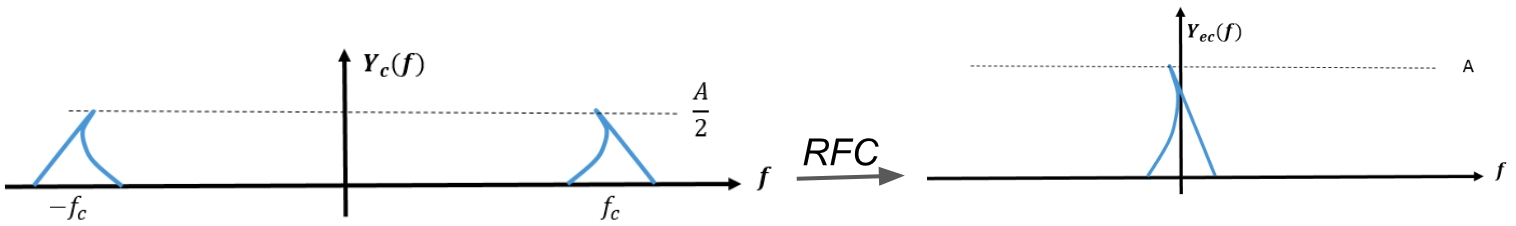
\includegraphics[scale=0.25]{Imagenes/rfconversion.jpg}
	\label{fig:RTC}
	%	\captionsetup{justification=raggedright,font={scriptsize,bf,it}}
	%	\caption*{fuente: llllll}
\end{figure}

\subsection{El Up Converter}
Puede verse como una solución práctica de la Conversión RF inversa y se presenta en la siguiente figura \\

\vspace{200px}
\begin{figure}[h!]
	\captionsetup{justification = raggedright, singlelinecheck = false}
	\caption{Up converter.\textcolor{red}{corregir: las fórmulas de la figura no se ha puesto como fórmulas}} 
	\centering
	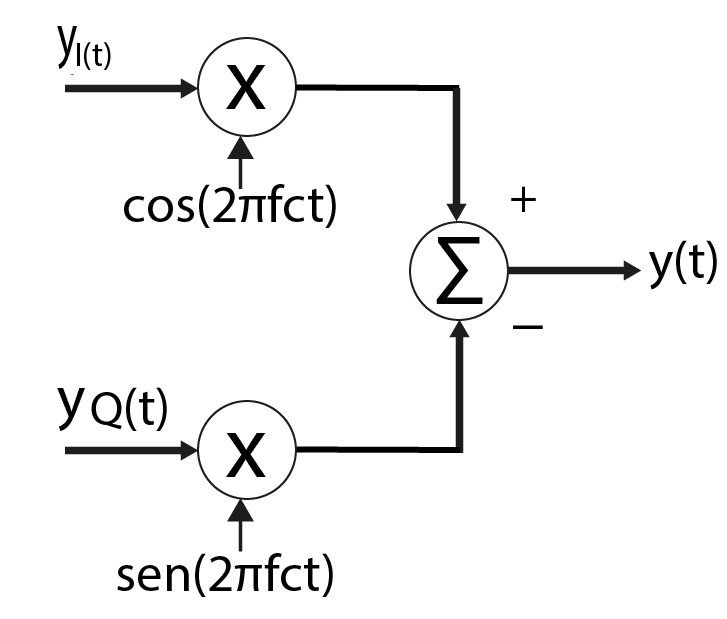
\includegraphics[scale=0.3]{Imagenes/Up.png}
	\label{fig:Up}
%	\captionsetup{justification=raggedright,font={scriptsize,bf,it}}
%	\caption*{fuente: llllll}
\end{figure}

\textbf{Ejercicio:} Hallar la expresión de la Envolvente Compleja de una señal FM paso bandas. Es bien sabido que la expresiòn matemàtica de una señal pasobandas FM es:\\

	\begin{equation} \label{capdos_cinco}
		s(t)= A_{c}\cos(2\pi(f_{c}+K_{f}m(t))t )  %\OR la expresión no es correcta
	\end{equation}

Donde, $A_{c}$ es la amplitud de la portadora, $f_{c}$ es la frecuencia de la portadora, $K_{f}$ es el coeficiente de modulación, $m(t)$ es el mensaje y $t$ es la variable de tiempo.\\

\textbf{Solución}: La siguiente figura presenta una forma hipotética de la TF de $s(t)$.\\

\begin{figure}[h!]
	\captionsetup{justification = raggedright, singlelinecheck = false}
	\caption{Espectro de señal paso bandas.} 
	\centering
	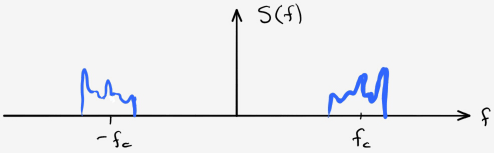
\includegraphics[scale=1]{Imagenes/Espectro-pasobanda.png}
	\label{fig:Espectro-pasobanda}
	%	\captionsetup{justification=raggedright,font={scriptsize,bf,it}}
	%	\caption*{fuente: llllll}
\end{figure}

Obtenemos la expresión para la señal $s(t)$ cuya TF es la misma $S(f)$ pero sin  la componente en frecuencias negativas, como  siguiente figura \\

\vspace{200px}
\begin{figure}[h!]
	\captionsetup{justification = raggedright, singlelinecheck = false}
	\caption{Espectro de la Pre envolvente compleja.} 
	\centering
	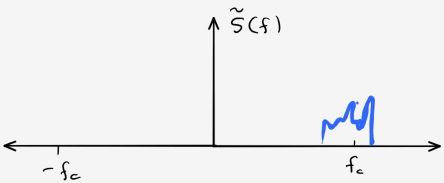
\includegraphics[scale=1]{Imagenes/Espectro-pre.png}
	\label{fig:Espectro-pre}
	%	\captionsetup{justification=raggedright,font={scriptsize,bf,it}}
	%	\caption*{fuente: llllll}
\end{figure}

$s(t)= \frac{1}{2}A_{c}e^{j(2\pi(f_{c}+K_{f}m(t)t))}.$ Esta expresión debe multiplicarse por 2 para conservar la energía, con lo cual se obtiene la pre-envolvente compleja. Hacemos $f_{c}=0$ y obtenemos la Envolvente Compleja.\\ 

\begin{equation} \label{capdos_seis}
	Sec(t)= A_{c}e^{j(2\pi(K_{f}m(t))t)} = A_{c}\cos(2\pi 0K_{f}m(t)t) + jA_{c}\sin(2\pi 0K_{f}m(t)t) 
\end{equation}

Esta es a su vez la fórmula de la FM bandabase. En principio, a cualquier señal pasobandas le corresponde una versión bandabase , que es su envolvente compleja. Podemos ver que la envolvente compleja de una señal FM es un vector rotante. En el sitio web del libro se brindan más detalles en forma de vídeos demostrativos sobre Envolvente Compleja y Up converter.\\

\begin{center}
\url{https://sites.google.com/saber.uis.edu.co/comdig/m/ec} 
\end{center}

\subsection{El Down Converter}

Para obtener la Envolvente Compleja de una señal paso bandas, se usa un dispositivo que llamaremos “Down converter” y que se presenta en la siguiente gráfica: \\

%\vspace{100px}
\begin{figure}[h!]
	\captionsetup{justification = raggedright, singlelinecheck = false}
	\caption{Tomado del Libro de Haykin, cap 1.11.} 
	\centering
	\includegraphics[scale=0.3]{Imagenes/libro-haykin.png}
	\label{fig:libro-haykin}
%	\captionsetup{justification=raggedright,font={scriptsize,bf,it}}
%	\caption*{fuente: http://youtu.be/h-rseLrniCk}
\end{figure}

La envolvente compleja es la señal $y_{c}(t) =  y_{I}(t) + j y_{Q}(t)$,  $y_{I}(t)$ es conocida como la componente en fase,  $y_{Q}(t)$ como la componente en cuadratura de la Envolvente Compleja.

\subsubsection{Demostración del Down Converter}

La Transformada de Fourier es una herramienta útil para diseñar y demostrar la validez de este tipo de soluciones.\\

\begin{equation} \label{capdos_siete}	
y(f)= \frac{1}{2}[y_{ec}(f-f_{c})+y_{ec}(-f-f_{c})]
\end{equation}

\begin{equation} \label{capdos_ocho}
y_{CI}(t) = y_{c}(t)2\cos (2\pi f_{c}t) \Longrightarrow y_{CI}(t) = y_{c}(f-f_{c})+y_{c}(f+f_{c}) 
\end{equation}

\begin{equation} \label{capdos_nueve}
y_{CI}(f) = \frac{1}{2}  [y_{ec}(f-2f_{c}) + y_{ec}(-f) + y_{ec}(f)+y_{ec}(-f-2f_{c})]
\end{equation}

\begin{equation} \label{capdos_diez}
y_{I}(f) = \frac{1}{2}[y_{ec}(-f) + y_{ec}(f)]
\end{equation}

\begin{equation} \label{capdos_once}
y_{CQ}(t) = -2y_{c}(t)\sin (2\pi f_{c}t)  \Longrightarrow TF y_{CQ}(f)= \frac{-1}{2j} [y_{c}(f-f_{c})-y_{c}(f+f_{c})]
\end{equation}

\begin{equation} \label{capdos_doce}
y_{CQ}(f) = \frac{-1}{2j} [y_{ec}(f-2f_{c}) + y_{ec}(-f) - y_{ec}(f)- y_{ec}(-f-2f_{c})]
\end{equation}

\begin{equation} \label{capdos_trece}
y_{Q}(f) = \frac{1}{2j} [y_{ec}(f)- y_{ec}(-f)]
\end{equation}

De modo que el sistema de la figura \ref{fig:libro-haykin} permite obtener la componente en fase y cuadratura de la Envolvente Compleja $y_{ec}(t) \Longrightarrow  y_{ec}(f)$

\subsubsection{Demostración gráfica del Down Converter}

Aplicaremos el Down Converter de la figura \ref{fig:Up} a la señal que tiene la TF de la figura \ref{fig:Espectro-bandapaso}. Deberemos obtener la TF de la Envolvente Compleja que es la que aparece en la figura \ref{fig:Espectro}.

%\vspace{100px}
\begin{figure}[h!]
	\captionsetup{justification = raggedright, singlelinecheck = false}
	\caption{Resultado del uso del Down Converter} 
	\centering
	\includegraphics[scale=0.9]{Imagenes/resultado.png}
	\label{fig:resultado-down}
%	\captionsetup{justification=raggedright,font={scriptsize,bf,it}}
%	\caption*{fuente: http://youtu.be/h-rseLrniCk}
\end{figure}


\subsection{La Envolvente compleja. Sus características}
\subsubsection{El problema a resolver}

A continuación se enuncia un problema que justifica el uso de este concepto.\\

Deseamos implementar un analizador de espectros  en un computador portátil mediante una aplicación basada en la FFT. Observar el espectro de la voz usando la FFT no representa un gran problema. Necesitamos conectar un micrófono al computador, el cual tiene un ancho de banda que finalmente establece una frecuencia máxima para la voz. Cumpliendo el Teorema de Nyquist, la señal de voz deberá ser muestreada a la frecuencia de muestreo \\ 

\begin{equation} \label{capdos_catorce}
f_{s} \geq 2f_{max} = 30KHz
\end{equation}

EL problema se complica cuando se desea analizar la señal que proviene de la radio base de un operador móvil. Será necesario conectar un receptor que convierte la señal electromagnética en una señal eléctrica y la amplifica de manera suficiente. \\ 

%\vspace{200px}
\begin{figure}[h!]
	\captionsetup{justification = raggedright,singlelinecheck = false}	
    \caption{Analizador de espectros basado en computador.} 
    \label{fig:Analizador}
    \centering
    \includegraphics[trim = 0mm 0mm 0mm 0mm, clip,width=1\textwidth]{Imagenes/Analizador}
	\par
		\captionsetup{justification=raggedright,font={scriptsize,bf,it}}
		\caption*{fuente: Autor}
\end{figure}

Pero ahora tenemos una frecuencia máxima muchísimo mayor, por ejemplo 1900000000 Hz. De modo que el muestreo resulta ahora extremadamente costoso y la FFT debe desarrollar tantas operaciones que el espectro no podrá ser visto en tiempo real. \\ 

\subsubsection{La solución. La Envolvente compleja}

{\setlength{\parindent}{1pt}La solución lógica consiste en incluir dentro  del receptor un dispositivo que permita desplazar el espectro de la señal de interés para centrarlo en una frecuencia mucho más baja a la que estaba centrado originalmente. El caso más extremo se tiene cuando el receptor logra centrar el espectro en $f_{c}$= 0 Hz.}  \\ 

{\setlength{\parindent}{1pt} En la siguiente gráfica se representa un ejemplo de la Transformada de Fourier de la señal de interés }

\vspace{200px}
\begin{figure}[h!]
	\captionsetup{justification = raggedright, singlelinecheck = false}
	\caption{Espectro de la señal pasobandas de interés.} 
  	\label{fig:Espectro-bandapaso}
	\centering
	\includegraphics[trim = 0mm 0mm 0mm 0mm, clip,width=1\textwidth]{Imagenes/Espectro-bandapaso.png}
	%	\captionsetup{justification=raggedright,font={scriptsize,bf,it}}
	%	\caption*{fuente: llllll}
\end{figure}


{\setlength{\parindent}{1pt}En la figura \ref{fig:Espectro-bandapaso}, el espectro es simétrico alrededor de la frecuencia $f = 0 Hz$, por lo tanto pertenece a una señal real. Sin embargo, alrededor de la frecuencia fc no es simétrico lo cual es usual  en las comunicaciones. 
En la figura \ref{fig:Espectro} se muestra el resultado al que queremos llegar, donde el espectro aparece centrado en $f_{c}=0 Hz$. Tiene doble amplitud que el de la  figura \ref{fig:Espectro-bandapaso}, con el fin de que conserve la misma energía.} \\ 

\begin{figure}[h!]
	\captionsetup{justification = raggedright, singlelinecheck = false}
	\caption{Espectro de la Envolvente Compleja.} 
	\centering
	\includegraphics[scale=1.2]{Imagenes/Espectro-envolvente.png}
	\label{fig:Espectro}
	%	\captionsetup{justification=raggedright,font={scriptsize,bf,it}}
	%	\caption*{fuente: llllll}
\end{figure}

{\setlength{\parindent}{1pt}Pero ahora el espectro no es simétrico, luego pertenece a una señal compleja que llamaremos Envolvente Compleja.Puede decirse que la Envolvente Compleja es la señal que resulta en el dominio del tiempo al desplazar el espectro de una señal paso bandas de interés que está centrado en una frecuencia $f_{c}$ $>$ 0 para que quede centrado en la frecuencia  $f_{c}$= 0 Hz, sin que se afecte la forma del espectro y por lo tanto sin que se afecte la información que está contenido en él.}\\

\subsection{El uso de la envolvente compleja en la simulación de Sistemas de comunicaciones}

El problema que en este caso justifica el uso de la Envolvente Compleja es el siguiente: supongamos que un operador móvil tiene instalada una red de datos inalámbrica por toda la ciudad y ahora desea cambiar el sistema de comunicación usado a otro. Por ejemplo, pasar de 2G a 3G.  Bien podría reutilizar la red de radio ya instalada. Entonces solo adquirir comparar la sección de equipos que procesa la Envolvente Compleja, que a menudo también se conoce como la señal banda base o componente en fase y en cuadratura ó señal I y señal Q. La sección de radio, en la parte transmisora, se encarga de obtener la señal paso bandas a partir de la envolvente compleja. En la parte receptora, esta sección se encarga de obtener la señal banda base a partir de la paso bandas. En otras palabras, la sección de radio incorpora un up-converter en la parte transmisora y un down-converter en la parte receptora. \\

\vspace{100px}
%\setcounter{figure}{11}
\begin{figure}[h!]
	\captionsetup{justification = raggedright, singlelinecheck = false}
	\caption{Esquema de Modulación pasobandas usando SDR} 
	\centering
	\includegraphics[scale=0.3]{Imagenes/Envol-GNU.png}
	\label{fig:Envol-GNU}
	%	\captionsetup{justification=raggedright,font={scriptsize,bf,it}}
	%	\caption*{fuente: http://youtu.be/h-rseLrniCk}
\end{figure}

En GNU Radio, la EC sólo puede generarse, observarse y recibirse en forma de una señal discreta. Esto obliga a tener ciertos cuidados principalmente relacionados con la frecuencia de muestreo. Los siguientes son puntos a tener en cuenta:\\

\begin{itemize}
	\item [$\bullet$] El modelo matemático de la EC en forma discreta es: $S_{ec}(t) = A[n]e^{j[2\pi B(n)n/B +Q(n) ]}$ y es de esta forma que puede ser implementado el modulador. El parámetro $N$ está relacionado con la frecuencia de muestreo samp-rate y este último con el tiempo continuo, así: \\
	$samp-rate=T/N$, donde $T$ es el periodo de la frecuencia máxima que puede tener la señal y $N$ es el número de muestras en ese periodo.
	\item [$\bullet$] Algunos bloques pueden producir la fórmula anterior, sin que el programador tenga que ver con esa expresión, por ejemplo el bloque Signal Source, pide parámetros continuos como la amplitud, la frecuencia y por supuesto la frecuencia de muestreo.
	\item [$\bullet$] Un modulador usualmente usa solo uno o dos de los anteriores parámetros de modo que la ecuación se puede simplificar en varias formas como las siguientes:	
	\begin{itemize}
		\item [$\bullet$] Cuando solo varía la magnitud: $S_{ec}(t)= A[n]$	
		\item [$\bullet$] Cuando solo varía la fase: $S_{ec}(t)= e^{jQ(n)}$
		\item [$\bullet$] Cuando varía fase y amplitud: $S_{ec}(t) = A[n]e^{jQ(n)}$
		\item [$\bullet$] Cuando solo varía la frecuencia: $S_{ec}(t) = e^{j2\pi B(n)n/N }$
	\end{itemize}
   
	\item [$\bullet$] Luego del modulador, al interior del USRP se cuenta con un elemento que llamamos “Complex to Real” que convierte la EC en dos señales, la señal I y la señal Q, también conocidas como señal en fase y señal en cuadratura.
	\item [$\bullet$] Esas dos señales entran luego a un DAC donde se convierten en señales eléctricas continuas. Es aquí donde la frecuencia de muestreo de la señal que se entrega al DAC juega un gran papel para llegar a producir de manera apropiada esas señales continuas. Básicamente debe cumplirse el Teorema de Nyquist.	
	\item [$\bullet$]Puede decirse que a la salida del DAC se tiene la EC en forma continua, pero en forma de dos señales reales, la señal I y la señal Q.
	\item [$\bullet$] Finalmente, el Up Converter aplica en el plano continuo lo que arrima hemos llamado Conversión RF.
\end{itemize}

En la parte receptora ocurre algo similar en sentido contrario . \\


\subsection{Simulación de señales y sistemas de comunicación en versión bandabase}

Es similar a lo explicado anteriormente, pero el canal también se simula en versión banda base de modo que no se hace necesario incluir un Up Converter ni un Down Converter. De esta manera, es posible hacer simulación con resultados similares pero a un costo computacional sensiblemente menor ya que el uso de esos conversores demanda la necesidad de incluir un sobremuestreo que depende de qué tan alta sea la frecuencia de la portadora.

\subsubsection{El ruido blanco en versión bandabase}
Como ya se ha estudiado, el uso de gnuradio para por usar un software un hardware que para nuestro caso es un equipo USRP y que su elemento principal es un Down Converter, si hablamos de la parte receptora o un Up Converter si hablamos de la parte transmisora. Los aspectos a tener en cuenta son los siguientes:

\begin{itemize}
	
	\item [$\bullet$] Sabemos que el Down Converter se encarga de recibir una señal pasobandas y entregar una señal banda base. Pero el Down Converter también tiene un ancho de banda limitado, de modo que, si a la entrada del Down Converter se tiene una señal de ruido blanco, este solo va a reconocer lo que esté dentro del ancho de banda que tenga configurado. Por eso se habla de ruido blanco de banda angosta (NBWN, del inglés Narrow Band White Noise).
	\item [$\bullet$] Podemos deducir que la salida del Down Converter es la Envolvente Compleja del NBWN y lo podemos llamar Ruido Blanco banda base (BBWN). 
	\item [$\bullet$] También vale la pena recordar que la PSD de la Envolvente Compleja tiene una altura 2 veces mayor a la PSD de la señal pasobandas, aunque esto puede ser no muy notorio si se usa la PSD está dada en dB.
	\item [$\bullet$] 	Es posible deducir que el ruido blanco de banda angosta ya no goza de las mismas propiedades del ruido blanco, así: el ancho de banda ya no es infinito, la función de autocorrelación ya no tiene la forma de una función delta, ni es lo último en aleatoriedad. Lo único que se mantiene es que la altura de la PSD es igual a $\dfrac{N_0}{2}$. 
\end{itemize}

Para analizar todo usando GNU Radio, hemos modificado el flujograma ya visto para obtener el flujograma “La-FFT-Ruido blanco banda base y paso bandas.grc”, que se muestra en la siguiente figura.

\vspace{300px}
\begin{figure}[h!]
	\captionsetup{justification = raggedright, singlelinecheck = false}
	\caption{Flujograma “La-FFT-Ruido blanco banda base y paso bandas.grc” para comparar el ruido blanco con el ruido blanco de banda angosta en banda base} 
	\centering
	\includegraphics[scale=0.7]{Imagenes/Ruido.png}
	\label{fig:Ruido}
%	\captionsetup{justification=raggedright,font={scriptsize,bf,it}}
%	\caption*{fuente: Tomado del libro de Haykin}
\end{figure}

Los resultados de este flujograma se presentan en la siguiente figura donde podemos ver lo siguiente:

\begin{itemize}
	
	\item [$\bullet$] Hemos puesto un generador de ruido blanco (WN, del inglés White Noise).
	\item [$\bullet$] El ruido blanco en toda su dimensión es imposible de ser observado o simulado, pero podemos obtener una versión con altura de PSD igual a $N_0/2=50 10^{6}$y una frecuencia de muestreo Fs-ruido-blanco=136 KHz, calculando que sea apenas lo suficiente para observar lo que puede ser de interés para nuestro caso. De allí, usando un Filtro Paso Bandas, con ancho de banda B = 8 kHz, hemos obtenido el Ruido Blando de Banda Angosta (NBWN, del inglés Narrow Band White Noise). 
	\item [$\bullet$] Los resultados muestran que, con el filtrado, la señal en el tiempo sufre una caída en la amplitud y su forma se vuelve más suave, pero se conserva la altura de la PSD.\\
	
	\vspace{400px}
	
	\begin{figure}[h!]
		\captionsetup{justification = raggedright, singlelinecheck = false}
		\caption{PDS y señal en el tiempo del ruido blanco (arriba). PSD de la Envolvente compleja ruido blanco de banda angosta y diagrama polar del mismo ruido} 
		\centering
		\includegraphics[scale=1]{Imagenes/Ruido-blanco.png}
		\label{fig:Ruido-blanco}
		%	\captionsetup{justification=raggedright,font={scriptsize,bf,it}}
		%	\caption*{fuente: Tomado del libro de Haykin}
	\end{figure}
	
	
	\item [$\bullet$] También hemos usado un generador de ruido blanco en versión compleja con amplitud $N_0=100 10^{6}$, para simular con él lo que debería producir el Down Converter
	\item [$\bullet$] El bloque Rational Resampler se agregó solo con el fin de observar qué hay más allá del ancho de banda bandabase BW=4 kHz. Los resultados, los vemos en la siguiente Figura 45, se trata de la Envolvente Compleja de ruido blanco, que también podemos llamar Ruido Blanco Bandabase. A la izquierda tenemos la PSD y a la derecha la gráfica en el dominio polar.
	
\end{itemize}

%\vspace{250px}
\begin{figure}[h!]
	\captionsetup{justification = raggedright, singlelinecheck = false}
	\caption{Ruido Blanco Banda Base, su PSD y representación Polar} 
	\centering
	\includegraphics[scale=1]{Imagenes/Polar.png}
	\label{fig:Polar}
	%	\captionsetup{justification=raggedright,font={scriptsize,bf,it}}
	%	\caption*{fuente: Tomado del libro de Haykin}
\end{figure}

\subsection{Un canal inalámbrico de ruido blanco gausiano aditivo en versión bandabase }
El canal de ruido blanco gaussiano aditivo es mejor conocido en inglés como Additive White Gaussian Noise Channel (AWGN Channel). Es bien sabido que una señal en su viaje desde una antena transmisora hasta una receptora atraviesa una gran cantidad de fenómenos. Es como si la señal entrara a un sistema que la deforma de varias maneras y ese sistema es lo que llamamos canal de propagación. Uno de ellos es el ruido y precisamente nos preparamos para revisar cómo luchar contra el efecto que este produce. Es muy claro que si vamos a probar un método para atenuar el ruido blanco, resulta importante poder aislar todos los demás fenómenos que pueden existir en el canal de propagación, de manera que el canal solo tenga la posibilidad de inyectar a la señal ruido blanco. Un esquema práctico es el que se muestra en la figura \ref{fig:Conformacion}.

\begin{figure}[h!]
	\captionsetup{justification = raggedright, singlelinecheck = false}
	\caption{Conformación de un canal pasobandas de ruido blanco.} 
	\centering
	\includegraphics[scale=1]{Imagenes/Conformacion.png}
	\label{fig:Conformacion}
%	\captionsetup{justification=raggedright,font={scriptsize,bf,it}}
%	\caption*{fuente: Tomado de Haykin}
\end{figure}

Como puede verse, el efecto del canal se expresa de la siguiente manera $ x_{w}(t) = x(t) + w(t)$ donde $ x(t) $  es la versión pasobandas y continua de la señal modulada en bandabase , $ x_{ec}[k], w(t) $  es el ruido blanco pasobandas. \\
Cuando se trata de explotar al máximo la posibilidades que ofrece el gnuradio, lo conveniente es crear un canal bandabase de ruido blanco que consiste en imitar prácticamente todos bloques que se tienen en la figura \ref{fig:Conformacion}. Para esto es importante tener en cuenta que la salida de ese canal es $ x_{nec}[k] = x_{ec}[k] + n_{ce}[k] $. \\

Donde $ n_{ce}[k] $ es la envolvente compleja en versión discreta de $n(t)$, el cual a su vez la porción del ruido $ w(t)$ que es admitida por el receptor ya que este tiene un ancho de banda finito y por tanto lo que deja pasar es más bien una señal de ruido blanco de banda angosta , que  llamaremos$  n(t) $. $ n_{ce} [k] $ es conocida también como Ruido Blanco de Banda Angosta en versión Bandabase y discreta. \\

En otras palabras, lo que resulta a la salida del ADC es la misma señal que entra al DAC pero con una adición de ruido blanco banda base , como se muestra en  la figura \ref{fig:Implementacion}, donde se tiene la implementación en GNU Radio de un canal de ruido blanco gaussiano aditivo.\\

\vspace{200px}
\begin{figure}[h!]
\captionsetup{justification = raggedright, singlelinecheck = false}
\caption{Implementación en GNU Radio de un Canal de ruido blanco aditivo.} 
\centering
\includegraphics[scale=1]{Imagenes/Implementacion.png}
\label{fig:Implementacion}
%	\captionsetup{justification=raggedright,font={scriptsize,bf,it}}
%	\caption*{fuente: Tomado de Haykin}
\end{figure}

En la figura \ref{fig:Implementacion}, el parámetro Amplitud, en el bloque Noise Source corresponde al valor RMS Vrms del ruido, el cual resulta relacionado con la potencia promedio P del ruido y con el valor No.  \\

En la figura \ref{fig:Diagrama-Polar} se muestra el ruido blanco de banda angosta en banda base, visualizado en un diagrama polar.

\begin{figure}[h!]
	\captionsetup{justification = raggedright, singlelinecheck = false}
	\caption{Ruido Blanco Bandabase en el Diagrama Polar.} 
	\centering
	\includegraphics[scale=1]{Imagenes/Diagrama-Polar.png}
	\label{fig:Diagrama-Polar}
	%	\captionsetup{justification=raggedright,font={scriptsize,bf,it}}
	%	\caption*{fuente: Tomado de Haykin}
\end{figure}

Como ya se dijo, el Ruido Blanco es una señal aleatoria teórica, de modo que resulta imposible generarlo en la práctica, pero tampoco resulta necesario generarlo de manera perfecta, pues un receptor, debido a sus limitaciones en ancho de banda solo deja pasar una porción del espectro de ese ruido. En todo caso, al pasar a bandabase, la PSD va a tener una altura constante igual a No, lo cual es fácil de deducir aplicando la Conversión RF vista en el capítulo 1.

\subsubsection{La modulación FM en versión bandabase}
\textcolor{red}{[Falta: Oscar Reyes]} %\OR a nivel de flujograma??
\subsubsection{La modulación AM en versión bandabase}
\textcolor{red}{[Falta: Oscar Reyes]}
%%%%%%%%%%%%%%%%%%%%%%%%%%%%%%%%%%%%%%%
%%%%%%%%%%%%%%%%%%%%%%%%%%%%%%%%%%%%%%%
\section{Ejercicios resueltos}
\subsection{Ejercicio 1}
\subsubsection{Enunciado}
\begin{enumerate}

\item Desde el punto de vista de GNU Radio, ¿de qu\'e tipo es la se\~nal que entrega el USRP receptor atrav\'es de un cable a la computadora?, será:
	\begin{enumerate}
      \item siempre una se\~nal real.
      \item siempre una se\~nal compleja.
      \item por lo general una se\~nal compleja.
	\end{enumerate}
    
\item Teniendo en cuenta que en GNU Radio la siguiente ecuaci\'on puede corresponder a una señal que se entrega a un bloque "UHD: USRP Sink"



\begin{equation} \label{capdos_quince}
S_{ec}[n] = A[n]e^{j(2 \pi  \beta[n]n/(N+Q[n]))}
\end{equation}

Conecte las ecuaciones de envolvente compleja con sus respectivas formas de modulaci\'on mediante una l\'inea recta, cuando en la señal que llega a la antena var\'ia s\'olo:

    \begin{figure} [h!] 
    \centering
    \includegraphics[width=0.7\textwidth]{Imagenes/Comu_1.png}
    \end{figure}

\item Sea la se\~nal $ y(t)=A_{1}\cdot x_{1}(t)\cdot \cos (2\pi ft)+ A_{2}\cdot x_{2}(t)\cdot \sin (2\pi ft+ m(t))$. C\'alcule su envolvente compleja. \\
\end{enumerate}


\subsubsection{Solución}

\begin{enumerate}
\item Rta: (b) Ser\'a siempre una se\~nal compleja.\\
Esto es debido a que el USRP receptor entrega una envolvente, de manera que la señal es inevitablemente compleja en su esencia. Incluso, aún cuando el transmisor emite cero en la parte imaginaria, al receptor llega un cierto ruido en esa parte imaginaria\\
\item Rta:
	\begin{figure} [h!] 
    \centering
    \includegraphics[width=0.7\textwidth]{Imagenes/Comu_1sol.png}
    \end{figure}


%\vspace{1em}
\item Aplicando la definición introducida en este libro de la Conversión RF directa en el dominio del tiempo tenemos:
\\

La definición de la Conversión RF nos indica que:
\begin{equation} \label{capdos_dieciseis}
 A(t)\cdot \cos (2\pi[ f_{0}+B(t)]+Q(t))  \overset{Conversion RF}{\rightarrow} A(t)\cdot e^{j[ \cdot 2\pi B(t)t+Q(t)]}
\end{equation}

Teniendo en cuenta esto, procedemos a calcular la envolvente compleja de la expresión planteada: 

\begin{equation} \label{capdos_diecisiete}
y(t)=A_{1}\cdot x_{1}(t)\cdot \cos (2\pi f_{0}t)+ A_{2}\cdot x_{2}(t)\cdot \sin (2\pi f_{0}t+ m(t))
\end{equation}

Aplicamos Conversión RF a cada termino de la expresión, identificando los parámetros que la conforman. Como lo es la amplitud, frecuencia, fase.\\

Para el término: 
\begin{equation} \label{capdos_dieciocho}
A_{1}\cdot x_{1}(t)\cdot \cos (2\pi ft)
\end{equation}

Encontramos que $A(t) = A_{1} \cdot x_{1}(t),\hspace{1em} f_{c}=f_{0} \hspace{1em} B(t)=0 \hspace{1em} y\hspace{1em} Q(t)=0$\\

Entonces:

\begin{equation} \label{capdos_diecinueve}
 A_{1}\cdot x_{1}(t)\cdot \cos (2\pi ft)  \overset{Conversion \ RF}{\rightarrow} \ 
 A_{1}\cdot x_{1}(t)
\end{equation}

Ahora, para el segundo término: 
\begin{equation} \label{capdos_veinte}
A_{2}\cdot x_{2}(t)\cdot \sin (2\pi f_{0}t+ m(t))
\end{equation}

Encontramos que contiene una función seno, dado que la Conversión RF solo es aplicable a funciones coseno es necesario expresar dicho seno en términos de coseno. Obteniendo el siguiente termino:
\begin{equation} \label{capdos_veintiuno}
A_{2}\cdot x_{2}(t)\cdot \cos (2\pi f_{0}t + m(t)-\pi/2)
\end{equation}

Al identificar los parámetros obtenemos que: \\$A(t) = A_{2} \cdot x_{2}(t),\hspace{1em} f_{c}=f_{0} \hspace{1em} B(t)=0 \hspace{1em} y\hspace{1em} Q(t)=m(t)-\pi/2$\\

Entonces:
\begin{equation} \label{capdos_veintidos}
 A_{2}\cdot x_{2}(t)\cdot \cos (2\pi f_{0}t + m(t) -\pi/2)  \overset{Conversion RF}{\rightarrow} A_{2}\cdot x_{2}(t)\cdot e^{j[ m(t)-\pi/2]}
\end{equation}
Teniendo la envolvente compleja de cada uno de los términos que comprenden y(t), los sumamos para construir su envolvente compleja, obteniendo el siguiente termino como resultado final.

\begin{equation} \label{capdos_veintitres}
 y_{ec}(t)=A_{1}\cdot x_{1}(t) + A_{2}\cdot x_{2}(t)\cdot e^{j[m(t)-\pi/2]}
\end{equation}

\end{enumerate}
%%%%%%%%%%%%%%%%%%%%
\subsection{Ejercicio 2}
\subsubsection{Enunciado}
\begin{itemize}
 \item[1)] Se tiene la siguiente expresión matemática de la envolvente compleja de una señal con modulación digital paso bandas:
 \end{itemize}
 
\begin{equation} \label{capdos_veinticuatro}
yec(t) = \left\lbrace
\begin{array}{ll}
\textup e^{j\pi /4}, m(t)=1  \\
\textup e^{j5\pi /4}, m(t)=0 
\end{array}
\right.
\end{equation}


\begin{itemize}
 \item[a)] Dibujar la EC de la forma polar que se obtendrá con GNU Radio en caso de usar muchísimas muestras por símbolo y graficarla de manera que parezca continua.
 \end{itemize}
 
\begin{itemize}
 \item[b)] Dibujar la EC de la forma polar para el caso en que ella ha sido muestreada, de forma que hay sólo una muestra por bit.
 \end{itemize}


\begin{itemize}
 \item[c)] Dibujar la señal paso bandas que corresponde a la EC dada para los siguientes bits:
 \\
 0 1 1 0
 \end{itemize}

\begin{itemize}
 \item[d)] Dibujar el flujograma gnuradio  para poder transmitir la señal al aire.
 \end{itemize}
 
 \begin{itemize}
 \item[e)] Graficar la forma de la señal en tiempo  que se obtiene en el receptor luego de pasar por el bloque USRP Source.
 \end{itemize}



\subsubsection{Solución}

 \begin{itemize}
 \item[a)]Se puede deducir de la expresión matemática que corresponde a la envolvente compleja de una BPSK, ya que tiene dos fases, una por cada símbolo digital que lleva.


 \begin{equation} \label{capdos_veinticinco}
 X1=45^{\circ}=\frac{\pi }{4} \; ; Para\; los\; unos.
 \end{equation}
 
 \begin{equation} \label{capdos_veintiseis}
 X2= \frac{5\pi }{4}=225^{\circ}; \;	Para\; los\; ceros.
 \end{equation}

%\vspace{100px} 
\begin{figure}[h!]
	\captionsetup{justification = raggedright, singlelinecheck = false}
	\caption{Gráfica de la forma polar continua de la envolvente compleja}
		\centering
    \includegraphics[width=0.8\textwidth]{Imagenes/polarcont.png}
    \label{fig:polarcont}
\end{figure}


\end{itemize}

 \begin{itemize}
 \item[b)] Desde el punto de vista teórico, la señal sólo tiene dos posibles valores, pero en la implementación en GNU Radio, la constelación tiene la forma de una línea debido a la transición cuando la señal pasa de un símbolo a otro.

\vspace{200px} 
 \begin{figure}[h!]
	\captionsetup{justification = raggedright, singlelinecheck = false}
    \caption{Gráfica de la forma polar discreta de la envolvente compleja}
    \centering
    \includegraphics[width=0.8\textwidth]{Imagenes/imagen1.jpg}
    \label{fig:imagen1}
\end{figure}

 \end{itemize}
 
\begin{itemize}
\item[c)] Para la realización de la señal paso bandas es necesario mirar la localización de los cambios de fase de la BPSK en la señal coseno, para saber de esta manera la posición del uno y del cero.

 \begin{figure}[h!]
	\captionsetup{justification = raggedright, singlelinecheck = false}
    \caption{figura de una señal senoidal con su respectiva fase}
    \centering
    \includegraphics[width=0.8\textwidth]{Imagenes/fas.PNG}
    \label{fig:fas}
\end{figure}

Otra manera de realizar la gráfica de la señal paso bandas es realizar el calculo mediante la Conversión RF. Mediante la cual se puede ver claramente cual es desfase de la señal para cuando tiene u valor de 1 o 0.
\\
\\
La siguiente es la definición de la Conversión RF:
 \begin{equation} \label{capdos_veintisiete}
A(t)cos(2\pi fc*t+B(t)+Q(t))\rightarrow A(t)e^{j(2\pi B(t)+Q(t))}
 \end{equation}
 Aplicando la Conversión RF a $y_{ec}(t)$, tenemos:
\\
Para m(t)=1
 \begin{equation} \label{capdos_veintiocho}
cos(2\pi fc*t+\pi /4)
\end{equation}
\\
Para m(t)=0
 \begin{equation} \label{capdos_veintinueve}
cos(2\pi fc*t+5\pi /4))
\end{equation}
\\

 \begin{figure}[h!]
	\captionsetup{justification = raggedright, singlelinecheck = false}
    \caption{Señal paso banda.}
    \centering
    \includegraphics[width=0.8\textwidth]{Imagenes/bit.PNG}
    \label{fig:bit-taller}
\end{figure}


\end{itemize}
 
\begin{itemize}
\item[d)]
 Para la realización de este punto se debe tener en cuenta que lo que se esta transmitiendo son bits que son apenas unos números discretos por consiguiente se necesita un wave forming que en este caso sera un retenedor de orden cero, el cual ayuda a que la señal consiga una forma cuadrada. Ver Figura \ref{fig:ejerciciodiagbloq}. El siguiente bloque corresponde a una constante de multiplicación la cual nos ayuda a atenuar o amplificar la señal según lo requiera el USRP, también se hace uso de un Rational Resampler el cual me permite cuadrar la frecuencia de muestreo a una que sea permitida por el USRP y por ultimo el USRP sink.
 
 \begin{figure}[h!]
	\captionsetup{justification = raggedright, singlelinecheck = false}
    \caption{Diagrama de bloques.}
    \centering
    \includegraphics[width=0.8\textwidth]{Imagenes/bloques.png}
    \label{fig:ejerciciodiagbloq}
\end{figure}

\end{itemize}



\begin{itemize}
\item[e)] La Señal en tiempo a la salida del USRP se presenta en la Figura \ref{fig:senalesperadausrp}.Cabe aclarar que la gráfica en GNU Radio no tendrá un aspecto como el de la imagen anterior sino que se observa una gráfica para la parte real, una para la imaginaria y una para la constelación, por aparte. 
\vspace{300px}
 \begin{figure}[h!]
	\captionsetup{justification = raggedright, singlelinecheck = false}
    \caption{Gráfica de la señal en tiempo que se espera a la salida del USRP.}
    \centering
    \includegraphics[width=0.8\textwidth]{Imagenes/finalll.png}
    \label{fig:senalesperadausrp}
\end{figure}



\end{itemize}

%%%%%%%%%%%%%%%%%%%%%%%%%%%%%%%%%%%%%%%
\subsection{Ejercicio 3}
\subsubsection{Enunciado}

Se tiene la señal paso banda mostrada en la figura 1. la cual fue obtenida en la entrada de una antena, cuando se deseó transmitir una señal digital. En ella se puede apreciar la forma en que están siendo representados los unos y ceros de la señal y la duración de cada bit.( $T_{b}=0.062ms$). Es importante tener en cuenta que pueden haber mas ciclos por símbolo.\\\\

%\vspace{300px}
 \begin{figure}[h!]
	\captionsetup{justification = raggedright, singlelinecheck = false}
    \caption{Señal pasobanda.}
    \centering
    \includegraphics[width=0.5\textwidth]{Imagenes/pasobanda.JPG}
    \label{fig:senaldeceros}
\end{figure}



Teniendo en cuenta lo anterior encuentre la representación polar  de la envolvente compleja de la señal dada.\\

Obtenga la gráfica  de  la PSD (Densidad espectral de potencia) de la señal dada con todas sus  especificaciones, calculando correctamente sus parámetros  para el caso en que la señal de la Figura 1 tiene asignado un canal inalámbrico entre 968 kHz y 1032 kHz.

\subsubsection{Respuesta}

 \begin{figure}[h!]
	\captionsetup{justification = raggedright, singlelinecheck = false}
    \caption{Señal pasobanda que representa a los unos.}
    \centering
    \includegraphics[width=0.6\textwidth]{Imagenes/unos.JPG}
    \label{fig:senaldeunos}
\end{figure}

\begin{equation} \label{capdos_treinta}
c_{1}(t)=5cos(2\pi ft+\frac{\pi}{2})
\end{equation}


 \begin{figure}[h!]
	\captionsetup{justification = raggedright, singlelinecheck = false}
    \caption{Señal pasobanda que representa a los ceros.}
    \centering
    \includegraphics[width=0.6\textwidth]{Imagenes/ceros.JPG}
    \label{fig:respuestadeunos}
\end{figure}

\begin{equation}  \label{capdos_treintauno}
c_{2}(t)=5cos(2\pi ft+\frac{3\pi}{2})
\end{equation}

La transformada Conversión RF directa nos señala que :

\begin{equation} \label{capdos_treintados}
A(t)cos\{2\pi(fc+B(t))t+Q(t)\}\longrightarrow A(t)e^{j(2\pi B(t)t+Q(t))}
\end{equation}
\\

En nuestro caso se tiene que:
\begin{align*}
A(t)=5
\end{align*}
\begin{align*}
B(t)=0
\end{align*}
\begin{align*}
fc=f
\end{align*}

\begin{equation} \label{capdos_treintatres}
Q(t)= \left\{ \begin{array}{lcc}
             \frac{\pi}{2} & = Para\ c_{1}(t) \\
             \\ \frac{3\pi}{2} & = Para\ c_{2}(t) \\
            
             \end{array}
   \right.
\end{equation}\\

Transformada Conversión RF para los unos se tiene:

\begin{equation} \label{capdos_treintacuatro}
c_{1}(t)=5cos(2\pi ft+\frac{\pi}{2})\longrightarrow 5e^{j\frac{\pi}{2}}
\end{equation}

Aplicando la transformada Conversión RF para los ceros se tiene:

\begin{equation} \label{capdos_treintacinco}
c_{2}(t)=5cos(2\pi ft+\frac{3\pi}{2})\longrightarrow 5e^{j\frac{3\pi}{2}}
\end{equation}



Envolvente compleja:

\begin{equation} \label{capdos_treintaseis}
Sec(t)= \left\{ \begin{array}{lcc}
             5e^{j\frac{\pi}{2}}   & = para los unos \\
             \\5e^{j\frac{3\pi}{2}} & = para los ceros \\
            
             \end{array}
   \right.
\end{equation}


 \begin{figure}[h!]
	\captionsetup{justification = raggedright, singlelinecheck = false}
    \caption{Envolvente compleja en un plano polar.}
    \centering
    \includegraphics[width=0.4\textwidth]{Imagenes/envolventecompleja.JPG}
    \label{fig:imagendepuntos}
\end{figure}


Calculo de la PSD 
\begin{equation*}
B= 1032kHz - 968kHz = 64 KHz 
\end{equation*} 
\begin{equation*}
Fc=968 kHz + B/2 =968 kHz +32 kHz=1000 kHz
\end{equation*}
\begin{equation*}
Rb=\frac{1}{Tb}=\frac{1}{0.062ms}=16kHz
\end{equation*}
\begin{equation*}
Nlobp=\frac{B}{Rb}=\frac{64kHz}{16KHz}=4
\end{equation*}

\vspace{200px}
 \begin{figure}[h!]
	\captionsetup{justification = raggedright, singlelinecheck = false}
    \caption{Grafica de la PSD.}
    \centering
    \includegraphics[width=0.8\textwidth]{Imagenes/PSDD.png}
    \label{fig:graficaPSD}
\end{figure}
%%%%%%%%%%%%%%%%%%%%%%%%%%%%%%%%%%%%%%%
\subsection{Ejercicio 4}
\subsubsection{Enunciado}
Se cuenta con un sistema de modulaci\'on pasobandas representado por la interconexi\'on de la figura 1. b(t) es una se\~nal de voltaje continuo que entrega 1V durante un periodo $T_{b}$ para se\~nalar los unos y 0V para se\~nalar los ceros.\\

%\vspace{200px}


 \begin{figure}[h!]
	\captionsetup{justification = raggedright, singlelinecheck = false}
    \caption{Sistema de modulaci\'on pasobandas.}
    \centering
    \includegraphics[width=0.6\textwidth]{Imagenes/1.png}
    \label{fig:imagenuno}
\end{figure}

Se tienen los siguientes par\'ametros:\

\[ c_{1}(t)=A_{1}Cos(2\pi f_{1}t) \]
\[ c_{2}(t)=A_{2}Cos[2\pi(f_{1}+\Delta f)t] \]
\[A_{1}=10V \]
\[A_{2}=10V \]
\[f_{1}=1000KHz \]
\[\Delta F=96KHz  \]
\[T_{b}=0,0625ms  \]
$b(t)$ lleva informaci\'on binaria: $ 1,1,0,1,0,0  $
\[B=192KHz \]

Nota: B es un ancho de banda pasobanda.
\begin{itemize}


 \item[a)] Grafique, en funci\'on del tiempo, las se\~nales $s_{1}(t)$,$ s_{2}(t)$ y s(t) para los datos dados. 
 
\item[b)] Grafique la PSD de s(t) se\~nalando todos los par\'ametros con cifras y unidades de medici\'on.
\item[c)] Grafique la envolvente compleja de la se\~nal s(t).
\subsubsection{Respuesta}
 \item[a)]  
Para la soluci\'on del enunciado lo primero que se debe hacer es un bosquejo de la se\~nal mensaje b(t), para ello se tiene en cuenta la informaci\'on binaria que da el enunciado: 1,1,0,1,0,0\
la se\~nal tendr\'ia la siguiente forma:

\vspace{20px}
 \begin{figure}[h!]
	\captionsetup{justification = raggedright, singlelinecheck = false}
    \caption{Mensaje transmitido.}
    \centering
    \includegraphics[width=0.4\textwidth]{Imagenes/2.eps}
    \label{fig:mensajetrans}
\end{figure}

%\newpage
La se\~nal anterior tiene la forma de una codificaci\'on binaria NRZ unipolar en donde al recibir un 1 el flanco sube, mientras que con los ceros ocurre lo contrario. $T_{b}$ es el tiempo del bit.
\
 \item[*]El bosquejo de $s_{1}(t)$  es el resultado de multiplicar la portadora $c_{1}(t)$ por la se\~nal de entrada.

 \begin{figure}[h!]
	\captionsetup{justification = raggedright, singlelinecheck = false}
    \caption{Se\~nal $s_{1}(t)$ en el dominio tiempo }
    \centering
    \includegraphics[width=0.5\textwidth]{Imagenes/3.eps}
    \label{fig:dominiotiempo}
\end{figure}


 \item[*]De igual forma $s_{2}(t)$ es el resultado de multiplicar la portadora $c_{2}(t)$ por la se\~nal $b_{z}(t)$ la cual es la se\~nal resultante de pasar el mensaje por un extractor de ceros como el de la figura 4. \\
 
 \vspace{200px}
 
  \begin{figure}[h!]
	\captionsetup{justification = raggedright, singlelinecheck = false}
    \caption{Extractor de ceros.}
    \centering
    \includegraphics[width=0.6\textwidth]{Imagenes/4.png}
    \label{fig:extractoceros}
\end{figure}
 
El extractor de ceros b\'asicamente lo que hace es convertir los unos a ceros y los ceros a unos. La se\~nal $s_{2}(t)$ la apreciamos en la figura \ref{fig:ejerciciosenals2}.
 
  \begin{figure}[h!]
	\captionsetup{justification = raggedright, singlelinecheck = false}
    \caption{Se\~nal $s_{2}(t)$ en el dominio tiempo }
    \centering
    \includegraphics[width=0.6\textwidth]{Imagenes/6.eps}
    \label{fig:ejerciciosenals2}
\end{figure}

%\newpage
\item[*]Por \'ultimo, se obtiene la se\~nal s(t) que es la suma de $s_{1}(t)$ con $s_{2}(t)$ y se puede apreciar a continuaci\'on:

 \vspace{200px}
   \begin{figure}[h!]
	\captionsetup{justification = raggedright, singlelinecheck = false}
    \caption{Se\~nal s(t) en el dominio tiempo  }
    \centering
    \includegraphics[width=0.6\textwidth]{Imagenes/5.eps}
    \label{fig:ejerciciosenals}
\end{figure}

 
\item[b)]Para graficar la PSD lo primero que se debe hacer es calcular la rata de bits $R_{b}$.\\

\begin{equation} \label{capdos_treintasiete}
 R_{b}=\dfrac{1}{T_{b}}=\dfrac{1}{0.0625*10^{-3}}
\end{equation}

\textbf{Consideraciones para realizar las gráficas de PSD} 
\item[*] Para dibujar la PSD se debe tener en cuenta que el l\'obulo central vale por 2 y est\'a centrado en la frecuencia de portadora.
\item[*] Las PSD de $s_{1}(t)$ y de $s_{2}(t)$ ser\'an iguales pero estar\'an centradas en diferentes frecuencias .   
\item[*] La PSD de una se\~nal pasobandas compuesta por la suma de dos se\~nales de diferentes frecuencias de portadora: $f_{1}$ y $f_{2}$ se obtiene al sumar las PSD de $s_{1}(t)$ y $s_{2}(t)$. \

Teniendo en cuenta lo anterior, se calcula el n\'umero de l\'obulos que tendr\'a la PSD de cada una de las se\~nales $s_{1}(t)$ y $s_{2}(t)$. Se tiene un ancho de banda de 192KHz, el cual se debe repartir entre las dos se\~nales, por lo tanto el ancho de banda que ocupa cada se\~nal es de $ \dfrac{B}{2}.$

\begin{equation} \label{capdos_treintaocho}
 Nlob= \dfrac{ \dfrac{B}{2} }{R_{b}} 
 = \dfrac{ 96[KHz]}{16 [Kbps]} 
 = 6 
\end{equation}

Como se  mencion\'o anteriormente, la PSD de la se\~nal s(t) es el resultado de la suma de las PSD de $s_{1}(t)$ y $s_{2}(t)$; por esto, la PSD de s(t) tendr\'a 12 l\'obulos como se observa a continuaci\'on:

   \begin{figure}[h!]
	\captionsetup{justification = raggedright, singlelinecheck = false}
    \caption{PSD de la se\~nal s(t).}
    \centering
    \includegraphics[width=0.7\textwidth]{Imagenes/7.png}
    \label{fig:lobulos}
\end{figure}

Donde:

\[f_{1}=1000KHz \]
\[\Delta f=96KHz  \]
\[f_{2}= f_{1} + \Delta F=  1096 KHz \]

\item[c)] 
\textbf{CONSIDERANDOS}\\
La diferencia entre una se\~nal bandabase (envolvente compleja) y la correspondiente pasobandas se puede observar en las figuras 8 y 9.

 \begin{figure}[h!]
	\captionsetup{justification = raggedright, singlelinecheck = false}
    \caption{PSD banda base.}
    \centering
    \includegraphics[width=0.6\textwidth]{Imagenes/9.jpeg}
    \label{fig:lobuloconsi}
\end{figure}


 \begin{figure}[h!]
	\captionsetup{justification = raggedright, singlelinecheck = false}
    \caption{PSD pasobandas.}
    \centering
    \includegraphics[width=0.6\textwidth]{Imagenes/10.jpeg}
    \label{fig:lobulodos}
\end{figure}

%\newpage
Para encontrar la envolvente compleja a partir de la se\~nal s(t) se usa la transformada RF (Conversión RF) que se define de la siguiente manera:\

\begin{equation}  \label{capdos_treintanueve}
A(t) Cos[ 2\pi(fc + B(t)) t + Q(t)] \\\\
\dfrac{Conversion RF}{} > A(t) e^{j[ 2\pi B(t) t + Q(t)]}  
\end{equation}

Aplicando la transformada Conversión RF se tiene:

\begin{equation}  \label{capdos_cuarenta}
s(t) = c_{1}(t) +c_{2}(t)
\end{equation}

\begin{equation}  \label{capdos_cuarentayuno}
 c_{1}(t)= A_{1} Cos [2\pi  (fc-\dfrac{\Delta F}{2})]\: para \: b(t)=1 
\end{equation}

\begin{equation}  \label{capdos_cuarentaydos}
 c_{2}(t)= A_{2} Cos [2\pi (fc+\dfrac{\Delta F}{2})] \: para \: b(t)=0 
\end{equation}


En ambos casos $Q(t)=0.$ La expresi\'on de envolvente compleja viene dada por:


\begin{equation}  \label{capdos_cuarentaytres}
c_{1}ce(t)=  A_{1} e^{-j2\pi \dfrac{\Delta F}{2}} \end{equation}

\begin{equation}  \label{capdos_cuarentaycuatro}
c_{2}ce(t)=  A_{2} e^{j2\pi \dfrac{\Delta F}{2}}
\end{equation}

 
 
\item[*] En banda base, la se\~nal es un vector rotante a una velocidad $\hat{f_{1}}$ para los unos y  $\hat{f_{2}}$ para los ceros.\\

%\vspace{20px}
 
\begin{figure}[h!]
	\captionsetup{justification = raggedright, singlelinecheck = false}
    \caption{Envolvente compleja s(t) forma polar.}
    \centering
    \includegraphics[width=0.6\textwidth]{Imagenes/12.jpeg}
    \label{fig:Envol-polar}
\end{figure}


Como se mencion\'o anteriormente, la envolvente compleja tiene forma de exponencial compleja la cual se puede expresar de la siguiente manera:

\begin{equation}  \label{capdos_cuarentaycinco}
e^{jx} = cos x +j sen x 
\end{equation}

Por lo tanto, para dibujar la parte real de la envolvente compleja se parte de la se\~nal coseno de la \textcolor{Red}{figura 11}  y para dibujar la parte imaginaria de la envolvente compleja se parte de la se\~nal seno de la \textcolor{Red}{figura 12.} 
 
\begin{figure}[h!]
	\captionsetup{justification = raggedright, singlelinecheck = false}
    \caption{Se\~nal a partir de la cual se dibuja la parte real de la envolvente compleja.}
    \centering
    \includegraphics[width=0.8\textwidth]{Imagenes/15.jpeg}
    \label{fig:seno-ejercicio}
\end{figure}

\vspace{200px}
\begin{figure}[h!]
	\captionsetup{justification = raggedright, singlelinecheck = false}
    \caption{Se\~nal a partir de la cual se dibuja la parte imaginaria de la envolvente compleja.}
    \centering
    \includegraphics[width=1\textwidth]{Imagenes/16.jpeg}
    \label{fig:matlab-ejercicio}
\end{figure}

%\newpage 

Finalmente, se tiene que la envolvente compleja de la se\~nal s(t) es: 

\begin{figure}[h!]
	\captionsetup{justification = raggedright, singlelinecheck = false}
    \caption{Envolvente compleja s(t).}
    \centering
    \includegraphics[width=1\textwidth]{Imagenes/13.png}
    \label{fig:dos-senos}
\end{figure}

 
En la figura anterior, para no dibujar demasiados ciclos en $T_{b}$, la gr\'afica a sido simplificada a un ciclo en $T_{b}$, sin embargo en la pr\'actica hay $ \dfrac{\Delta F}{2} $ ciclos en $T_{b}$.
\end{itemize}

\chapter{Implementación de la Radio Definida por Software en sistemas de radiodifusión}

Este capítulo tiene el fin de estudiar lo que significa Software Defined Radio (SDR) y un tipo de hardware usado en SDR. Con el fin de lograr que el estudiante tenga contacto con un hardware real, hemos seleccionado el USRP-2920 de la empresa National Instruments, pero también se busca generalizar el conocimiento sobre ese hardware en forma de modelos más generales que le brinde al estudiante la capacidad de descubrir y comprender cualquiera de los tipos de hardware existentes. El mayor ènfasis se hace en que estudiante conozca lo que un hardware SDR representa. 

%%%%%%%%%%%%%%%%%%%%%%%%%%%%%%%%%%%%%%%%%%%%%%%

\section{Radio Definida por Software en Modo de Red}

El término Modo de Red o “modo Network” es muy usado en los productos de la empresa Ettus, la cual a su vez pertenece a National Instruments, pero este modo corresponde la configuración más común en los laboratorios experimentales por ser la solución más económica y a la vez más potente. Consiste en lograr un complemento perfecto entre un hardware SDR y un computador con el software apropiado. El término network es usado debido a que el hardware se conecta al computador usualmente por un puerto Giga Ethernet de manera directa. En principio, no se descarta que esa conexión sea por Wi-Fi o que los componentes estén ubicados en lugares remotos distantes entre sí, unidos por Internet, pero esto no es usual pues entre el hardware y el computador se requiere enviar información muy pesada en tiempo real. \\


%\setcounter{figure}{57}
\begin{figure}[h!]
	\captionsetup{justification = raggedright, singlelinecheck = false}
	\caption{Un sistema de comunicaciones punto a punto Full Duplex.} 
	\centering
	\includegraphics[scale=0.8]{Imagenes/Full-duplex.png}
	\label{fig:Full-duplex}
%		\captionsetup{justification=raggedright,font={scriptsize,bf,it}}
%		\caption*{fuente: http://superkuh.com/rtlsdr.html}
\end{figure}

\vspace{200px}
\begin{figure}[h!]
	\captionsetup{justification = raggedright, singlelinecheck = false}
	\caption{Un transceptor (en inglés Transceiver).} 
	\centering
	\includegraphics[scale=0.8]{Imagenes/Transceptor.png}
	\label{fig:Transceptor}
	%		\captionsetup{justification=raggedright,font={scriptsize,bf,it}}
	%		\caption*{fuente: http://superkuh.com/rtlsdr.html}
\end{figure}

USRP (Universal Software Radio Peripheral) es el término usado por la empresa Ettus para denominar el hardware de una solución SDR. Como se muestra en la figura anterior, en el USRP se concentra la componente hardware del sistema de comunicación y en el computador la componente del software. Lo que viaja por el cable que une estos componentes es precisamente la Envolvente Compleja, no sin antes ser adaptada al protocolo Ethernet.\\

Para los USRP que solo funcionan en modo Network, se usa una nomenclatura especial, se considera que pertenece a la serie Nx, donde la N significa Network y la x unos números seriales. Algunos ejemplos son:  USRP N200, USRP N210. Sin embargo, como la empresa Ettus fue adquirida por National Instruments (NI), esta empresa está usando otra nomenclatura como: NI USRP 2920, NI USRP 2921, NI USRP 2922, NI USRP 2930, NI USRP 2932. Ese cambio de nomenclatura es aplicado por NI para indicar que estos equipos funcionan con LabView que es la plataforma de NI que ahora incursiona en SDR. Una comunicación completa en Modo Network se presenta en la figura \ref{fig:Modelo-capas}.\\

\begin{figure}[h!]
	\captionsetup{justification = raggedright, singlelinecheck = false}
	\caption{Modelo de capas de un sistema de comunicación con USRP en Modo Network.} 
	\centering
	\includegraphics[scale=0.8]{Imagenes/Modelo-capas.png}
	\label{fig:Modelo-capas}
	%		\captionsetup{justification=raggedright,font={scriptsize,bf,it}}
	%		\caption*{fuente: http://superkuh.com/rtlsdr.html}
\end{figure}

%%%%%%%%%%%%%%%%%%%%%%%%%%%%%%%%%%%%%%%%%%%%%%%%%%%

\section{Un equipo SDR parara Modo de Red. El NI USRP-2920}

El NI USRP-2920 es un ejemplo típico de un hardware pensado en una solución de comunicación basada en SDR en modo network. vale la pena usarlo como ejemplo para conocer lo que este tipo de equipos usualmente contiene. \\

\begin{figure}[h!]
	\captionsetup{justification = raggedright, singlelinecheck = false}
	\caption{Foto del NI USRP-2920.} 
	\centering
	\includegraphics[scale=0.8]{Imagenes/USRP-2920.png}
	\label{fig:USRP-2920}
	%		\captionsetup{justification=raggedright,font={scriptsize,bf,it}}
	%		\caption*{fuente: http://superkuh.com/rtlsdr.html}
\end{figure}

Es importante, tener claro desde un comienzo que estos USRP son construidos por la empresa \underline{Ettus Research}. Pero esta empresa fue adquirida en el 2015 por la empresa National Instruments (NI). De esta manera se entiende por qué un mismo hardware tiene dos nombres diferentes: uno que le da Ettus y otro que le da NI. \textbf{Es asì como el NI USRP 2920 de National Instruments corresponde al USRP N210 de Ettus}, donde la N indica que se trata de un equipo que funciona en modo Network. El equipo viene un software de NI que permite configurar el equipo con el driver que le permite actuar como NI USRP 2920 o bien con el driver que le permite actuar como USRP N210. El primer caso se usa cuando el equipo se usa con LabView sobre Windows, mientras el segundo, con GNU radio sobre Ubuntu. \\

El	\textcolor{red}{\href{http://www.ni.com/pdf/manuals/375839a.pdf}{manual de este equipo, en este enlace}}, es suficiente para comprender lo que el equipo representa externamente, así como sus especificaciones técnicas y cuidados de uso. Nos detendremos más bien en el esquema interno.\\

\vspace{400px}
\begin{figure}[h!]
	\captionsetup{justification = raggedright, singlelinecheck = false}
	\caption{Modelo de capas del NI USRP 29xx visto por capas. En color naranja: bloques de software embebido. En color verde: Hardware con parámetros controlables por computador. Blanco: Hardware no controlable.} 
	\centering
	\includegraphics[scale=0.8]{Imagenes/Modelo-29xx.png}
	\label{fig:Modelo-29xx}
		\captionsetup{justification=raggedright,font={scriptsize,bf,it}}
			\caption*{fuente: FALTA \textbf{Nota:} Según el manual del NI-USRP 2920 no es claro que tenga un banco de filtros}
\end{figure}

En los siguientes capítulos, el término “Usuario P” se refiere a la persona que está sentada en el computador, desarrollando una aplicación en GNU radio o usando una para contactar el USRP. \\

\subsection{El receptor del NI USRP-2920}

Como puede apreciarse, la parte receptora consiste en una o dos antenas que son conectadas por el RF switch. En muchos USRP la señal pasa inmediatamente por un banco de filtros que resultan sintonizados mediante las órdenes que da el Usuario P desde la aplicación ubicada en el computador. La señal es luego amplificada en el Low Noise Amp. La señal sigue a un amplificador que puede ser configurado por el usuario P desde la aplicación. El esquema que sigue es lo que en el primer capítulo hemos llamado Down Converter, en el cual la frecuencia del Oscilador controlado por voltaje (VCO) puede ser configurada desde la aplicación, pero no los parámetros del Low Pass Filter, que tiene un ancho de banda fijo, inmodificable, de 20 MHz. \\
El Usuario P tampoco puede modificar los parámetros del Conversor Análogo Digital (ADC), que muestrea la señal a su entrada a una rata fija, invariable de 100 MS/s y además la cuantiza a 14 bits/muestra. El Usuario P debe jugar con la ganancia o la atenuación para poder aprovechar todos los 14 bits por muestra, pues la señal entrante es muy débil y no alcanzaría a levantarse de manera suficiente. Pero también es necesario tener en cuenta que una sobre amplificación puede crear también un problema, el de saturación, como se muestra en las siguientes dos figuras.

\begin{figure}[h!]
	\captionsetup{justification = raggedright, singlelinecheck = false}
	\caption{Señal a la entrada del cuantizador.} 
	\centering
	\includegraphics[scale=1]{Imagenes/Senal-entrada.png}
	\label{fig:Senal-entrada}
	%		\captionsetup{justification=raggedright,font={scriptsize,bf,it}}
	%		\caption*{fuente: http://superkuh.com/rtlsdr.html}
\end{figure}


\begin{figure}[h!]
	\captionsetup{justification = raggedright, singlelinecheck = false}
	\caption{Señal a la salida del cuantizador.} 
	\centering
	\includegraphics[scale=1]{Imagenes/Senal-salida.png}
	\label{fig:Senal-salida}
	%		\captionsetup{justification=raggedright,font={scriptsize,bf,it}}
	%		\caption*{fuente: http://superkuh.com/rtlsdr.html}
\end{figure}

Por esta razón, es ideal que la señal resultante después de la amplificación quede con magnitud 1 o incluso 0,8, ya que el rango dinámico del ADC es 1 Vp-p, para el caso del NI USRP 2920. Así, las amplitudes de la componente I y la Q se puede deducir de la magnitud $\sqrt{I_{max}^{2} + Q_{max}^{2}} = 1$.\\

\subsubsection{Cálculo de la frecuencia de muestreo para un NI USRP.}

La señal pasa luego a la FPGA (la tarjeta madre), donde está el OSP (Onboard signal processor) que tiene algunos elementos de procesamiento digital, filtra la frecuencia central, de modo que no aparezca allí un delta que corresponde a la portadora. Pero también en el OSP se le aplica a la señal una decimación, combinado con un filtrado digital, para bajar la rata de muestreo de la señal I/Q para que cumpla con los deseos del programador que especificará un ancho de banda deseado que, en términos de frecuencia de muestreo, resultará en un valor que para el NI USRP 292x está entre 200 kS/s y 25 MS/s. Debido a las limitaciones del computador y la calidad del cable usado para unir el USRP con el computador, el Usuario P puede considerar que el ancho de banda pasobandas está entre 200 kHz y 20 ó 25 MHz, como se muestra en la siguiente figura. \\


\begin{figure}[h!]
	\captionsetup{justification = raggedright, singlelinecheck = false}
	\caption{Ancho de banda real que puede alcanzar el NI USRP 2920 con respecto a las capacidades de la tarjeta hija} 
	\centering
	\includegraphics[scale=1]{Imagenes/Ancho-banda-real.png}
	\label{fig:Ancho-banda-real}
	%		\captionsetup{justification=raggedright,font={scriptsize,bf,it}}
	%		\caption*{fuente: http://superkuh.com/rtlsdr.html}
\end{figure}

Ese ancho de banda se puede configurar en los bloques digitales alojados en el OSP. Esto ocurre de manera indirecta, cuando el Usuario P selecciona un el Coeficiente de Decimación $K_{d}$ para el bloque Digital LPF/decimator con el fin de bajar la frecuencia de muestreo. Es importante tener en cuenta que, usualmente ese coeficiente es un número entero y a la vez potencia de 2, de modo que: \\

\begin{equation} \label{captres_uno}
 K_{d} =2^{m}, donde m es entero positivo. \end{equation}

Los experimentos desarrollados por el autor, con el NI USRP 2920, muestran que, aunque el sistema acepta cualquier valor entero que sea par y positivo para ese coeficiente, si no se escoge como se señaló, se deforma el espectro de la señal que sale del decimador respecto a la que recibe el decimador. \textbf{El autor también demostró que con el NI USRP 2920, hay un tope máximo para ese coeficiente y es 512.} Eso significa que así como el equipo tiene un tope máximo para la frecuencia de muestreo de 100 MSps, también tiene un tope mínimo de 195,3125 kS/s, ósea $100e^{6}/512$. Esto también significa que, el mínimo ancho de banda que el USRP captura en pasobandas es 195,3125 kHz, que equivale a 97,65625 kHz en bandabase. \\

La señal resultante es luego enviada por el cable gigabit ethernet. En conclusión, el USRP captura una señal en toda la banda de 40 MHz, pero la procesa para enviar a la Rx GNU App el ancho de banda que el Usuario P configure en función del Coeficiente de Decimación. También es claro que el usuario está obligado a realizar la decimación, ya que de otra suerte, estaría obligando al USRP a entregar una rata de muestras que no es soportada por el sistema que une el USRP con el computador, o incluso por la capacidad del mismo computador. \\

\vspace{250px}
\begin{figure}[h!]
	\captionsetup{justification = raggedright, singlelinecheck = false}
	\caption{Análisis en banda base de frecuencias de muestreo y anchos de banda que se manejan en el USRP 2920 en el modo de recepción.} 
	\centering
	\includegraphics[scale=0.3]{Imagenes/Analisis-banda.png}
	\label{fig:Analisis-banda}
	%		\captionsetup{justification=raggedright,font={scriptsize,bf,it}}
	%		\caption*{fuente: http://superkuh.com/rtlsdr.html}
\end{figure}

En la figura anterior, vemos que la frecuencia de muestreo de 100 MS/s que por defecto maneja el DAC está sobredimensionada con respecto al ancho de banda del filtro analógico paso bandas usado como parte del down converter que es de 20 MHz, para capturar una señal de hasta 40 MHz. Pero al programador le interesa. Pero esta a su vez está sobredimensionada con respecto a lo que puede realmente viajar por el cable Gigabit Ethernet, lo que puede procesar el computador y en general, por lo que en realidad desea el usuario P. \\

Los usuarios P que son principiantes cometen a menudo el error de usar un Kdno entero, el sistema lo puede aceptar, pero lo redondea hacia arriba, para obtener el valor entero, como consecuencia la frecuencia de muestreo que entrega el USRP puede ser un tanto mayor a la que el usuario cree que va a recibir, con lo cual se produce una inconsistencia entre la frecuencia de muestreo usada por el Usuario P y la que realmente es, con lo cual se pueden producir distorsiones de señal en los siguientes bloques que conecte. Es importante que el Usuario P se asegure que la frecuencia de muestreo que él ha programado es la que el USRP le entrega, para ello, el GRC, como herramienta de programación tiene una ventana de texto donde aparece la advertencia: Target sample rate: tantos MHz, Actual sample rate: tantos MHz. El primer valor es lo que el usuario programó, el segundo, lo que el sistema pudo dar. \\

En resumen, en recepción, cuando se desea capturar un ancho de banda B. \\

{\setlength{\parindent}{1pt}$B_{d}$ = 10 MHz \\}
\vspace{5px}
$samp-rate_{d}$ = $B_{d}$ \\
\vspace{5px}
samp-rate-usrp = 100 MSps \\
\vspace{5px}
$Kd_{max}$ = 512 \\
\vspace{5px}
$Kd_{d}$ = Parte entera de samp-rate-usrp / samp-rate-d. De manera que ocurre un redondeo hacia abajo Kd el menor valor entre Kd=512  y  $K_{d}$ = $2^{\log_{2}Kd_{d}} $ \\
\vspace{5px}
samp-rate = samp-rate-usrp/$K_{d}$ \\
\vspace{5px}
B= samp-rate \\

En transmisión, cuando se desea emitir un ancho de banda B. El proceso es el mismo con las siguientes aclaraciones:

\begin{itemize}
	\item [$\bullet$] samp-rate-usrp = 400 MSps
	\item [$\bullet$] $Kd_{max}$ : no lo conocemos. El autor supone que es 4 veces mayor al usado en recepción, ya que la frecuencia de muestreo en el transmisor es 4 veces mayor a la usada en recepción.
	\item [$\bullet$] Se supone que el transmisor realiza una interpolación en vez de una decimación. Si se quiere ser muy estricto en esto, lo que hay que hacer es:
	\begin{itemize}
		\item [$\bullet$] Calcular el coeficiente de interpolación como: $K_{i}=1/K_{d}$.
		\item [$\bullet$] Luego obtener $samp-rate = samp-rate-usrp*K_{i}$.
		\item [$\bullet$] Pero la verdad, lo anterior se puede saltar, pues igual resulta que: $samp-rate = samp-rate-usrp/K_{d}$.
		
	\end{itemize}
\end{itemize}

\subsection{El transmisor del NI USRP-2920}

Puede entenderse de manera similar al receptor. \\


{\setlength{\parindent}{1pt}En cualquier desarrollo que se realice con SDR es importante conocer en detalle las especificaciones del equipo. Para tener una idea de lo que esto representa, analizaremos a continuación las especificaciones del NI USRP-2920.} \\

\begin{itemize}
	\item [$\bullet$] Para una consulta más precisa, consultar el \textcolor{red}{\href{http://www.ni.com/pdf/manuals/376358a.pdf}{manual del equipo}}
	\item [$\bullet$] El ancho de banda analógico es de 20 MHz analógico, pero esto equivale en pasobandas a 40 MHz. Además entra en juego el ADC, que muestrea a una rata fija, invariable de 400 MS/s la señal y la cuantifica a 16 bits/muestra.
\end{itemize}


\begin{figure}[h!]
	\captionsetup{justification = raggedright, singlelinecheck = false}
	\caption{Elementos internos del USRP para la transmisión.} 
	\centering
	\includegraphics[scale=1]{Imagenes/Elementos-internos.png}
	\label{fig:Elementos-internos}
%	\captionsetup{justification=raggedright,font={scriptsize,bf,it}}
%	\caption*{fuente: https://www.ettus.com/content/files/USRP-E310-Product-Sheet.pdf \\
%		Nota: no es claro que el NI USRP 2920 tenga un banco de filtros como estos, pues no aparecen en los manuales}
\end{figure}

{\setlength{\parindent}{1pt}En la figura XXX se observa que en modo transmisión, el USRP usa un DAC con una frecuencia de muestreo de 400 MS/s. También se observa que cuenta con el bloque Digital Interpolator para adaptar la frecuencia de muestreo de la señal que le llega.  Pero al igual que ocurrió con el coeficiente de decimación, en el modo recepción, aquí el coeficiente de interpolación también en obligatoriamente un número entero de la forma:}

\begin{equation} \label{captres_dos}	
K_{i} = 2^{m}, donde m es entero positivo. 
\end{equation}


\subsection{El papel de GPS en un NI USRP.}

El papel del GPS consiste en usar una señal satelital, del sistema GPS para lograr que el VCO de cualquiera de los varios equipos genere una misma senoidal. Esto mejora enormemente la recepción de una señal transmitida con otro USRP similar, ya que no se presenta desfase entre la portadora usada en el transmisor y en el receptor. Pero esta opción solo la tienen los NI USRP-293x.\\

\subsection{Los filtros en un NI USRP.}

\subsection*{En la parte receptora} 
La siguiente figura presenta un ejemplo de la respuesta en frecuencia del banco de filtros, como no se tenía en el momento la información para el NI USRP 2920, se presenta la del NI USRP E-310, para que el lector tenga una idea de lo que ese banco de filtros significa.

\begin{figure}[h!]
	\captionsetup{justification = raggedright, singlelinecheck = false}
	\caption{Banco de Filtros de la parte receptora del NI USRP E-310.} 
	\centering
	\includegraphics[scale=1]{Imagenes/Banco-filtros.png}
	\label{fig:Banco-filtros}
			\captionsetup{justification=raggedright,font={scriptsize,bf,it}}
			\caption*{fuente: https://www.ettus.com/content/files/USRP-E310-Product-Sheet.pdf \\
			Nota: no es claro que el NI USRP 2920 tenga un banco de filtros como estos, pues no aparecen en los manuales}
\end{figure}

El filtro a usar es seleccionado directamente por el Usuario P.\\

A manera de resumen, las especificaciones del receptor del NI USRP-2920 son  las siguientes: \\

\begin{itemize}
	\item [$\bullet$] La información más confiable sobre las especificaciones es la del	\textcolor{red}{\href{http://www.ni.com/pdf/manuals/376358a.pdf}{manual del equipo}}.
	\item [$\bullet$] Rango de frecuencias de 50 MHz a 2.2 GHz. (las bandas de radio FM, GPS, GSM, radar, ISM)
	\item [$\bullet$] Pasos de frecuencia $<$ 1 kHz
	\item [$\bullet$] Se usa un ADC de dos canales: 100 MS/s a 14 bits/muestra. Un canal es para la señal I y el otro para la señal Q, como se deduce de este \textcolor{red}{\href{http://www.ni.com/white-paper/13881/en/}{enlace}}
	\item [$\bullet$] El rango dinámico del ADC es 1 Vp-p. La potencia de entrada al ADC es no lineal pues varía con la frecuencia.
	\item [$\bullet$] Rata máxima real de muestreo I/Q: 25 MS/s a 16 bits/muestra; 40 MS/s a 8 bits/muestra. El manual aclara que este valor puede verse limitado aún más por las limitaciones del computador usado y por la velocidad de la conexión entre el USRP y el computador. A diferencia de la frecuencia de muestreo del ADC,este valor se refiere a la rata de muestreo a la que realmente puede funcionar el sistema en tiempo real. En otras palabras, si se intentara aprovechar los 100 MS/s que entrega el ADC, veríamos que el sistema se bloquearía o produciría errores, debido a que esa velocidad no es soportada por los bloques que siguen. 
	\item [$\bullet$] Ancho de banda máxima real: 20 MHz para 16 bits/muestra; 40 MHz para 8 bits/muestra.
	\item [$\bullet$] Nota 2: se deduce también que el Ancho de banda máxima instantánea en tiempo real, es el valor pasobandas que en términos reales se puede alcanzar, que representaremos como B. De modo que en bandabase, el ancho de banda es BW=B/2. Así toma sentido la frecuencia de muestreo que es Fs=2*BW=B. Por eso, vemos que en el caso de 8 bits/muestra, con 40 MS/s se alcanza un ancho de banda de 40 MHz. Eso es lo máximo que el equipo permite. Pero el Front-End al que tiene acceso el usuario P, es decir, el GRC, puede no tener la opción para programar este valor de 8 bits/muestra.
	\item [$\bullet$] El usuario P usualmente necesita un menor valor para la frecuencia de muestreo que entrega el USRP Source. Para satisfacer esa necesidad, el USRP Source cuenta con un diezmador. El problema es que el factor de diezmado no es cualquiera, sino que se aproxima al valor más cercano entre los siguientes: 8, 16, 32, 64, 128, 256, 512. 
\end{itemize}

Otras notas de interés para configurar el bloque de GNU radio conocido como USRP Source: \\

\begin{itemize}
	\item [$\bullet$] Para los usuarios P de Simulink es un poco confuso que el muestreo sea realizado por el ADC. Esto se entiende mejor si imaginamos que el ADC del usrp junto con el procesado que realiza luego el OSP, equivalen en Simulink a la interconexión de los bloques: filtro paso bajas, muestreador (con el bloque zero order hold), cuantizador (en caso de que la salida del USRP source sea configurada para  tipo entero). De modo que ADC+OSP lo que entregan es una señal, que usualmente veremos como una señal de valores decimales con un número finito de posibles valores. En otras palabras es la envolvente compleja de la señal que el usuario P desea capturar, pero en su versión muestreada y cuantizada, por lo tanto, esta señal pertenece al mundo físico.
	\item [$\bullet$] En Simulink de Matlab, el bloque USRP Source no pide frecuencia de muestreo sino coeficiente de decimación.
	\item [$\bullet$] El valor máximo de frecuencia de muestreo que se pudo programar sin problemas con un computador Core i7 fue de  fue de 20 MSps, que equivale a un ancho de banda pasobandas de 20 MHz. Pero con advertencias puede ser de 25 MSps. Teóricamente, con computadores mejor dotados se podría elevar más, pero sin pasar nunca de 50 MSps.
	\item [$\bullet$] Aunque la documentación dice que la frecuencia de muestreo cambia en función de número de bits por muestra que se elija, vimos que al menos el bloque USRP Source no brinda esta opción.
	\item [$\bullet$] Si el parámetro Ch0: Bandwidth se deja en cero, el ancho de banda del receptor usrp se sintoniza por defecto a una frecuencia cercana a la frecuencia de muestreo, porque se aplica el Teorema de Nyquist en versión bandabase.
	\item [$\bullet$] Otros parámetros del receptor del USRP de la serie N2920 son:
	\begin{itemize}
		\item [$\bullet$] La letra “N” se refiere a “Network”, debido a que usa puerto Gigabit  Ethernet para la unión PC-USRP
		\item [$\bullet$] La velocidad de los datos entre el PC y el USRP por el puerto Ethernet es de hasta 50 MS/s
		\item [$\bullet$] Se pueden unir varios USRP como si fuesen uno solo para escalar en capacidad
	\end{itemize}
\end{itemize}

\subsection{En la parte transmisora}
De manera similar, en la parte transmisora puede tenerse un banco de filtros como es el caso del NI USRP E-310, como se muestra en la Figura \ref{fig:Banco-e310}

\vspace{300px}
\begin{figure}[h!]
	\captionsetup{justification = raggedright, singlelinecheck = false}
	\caption{Banco de Filtros de la parte transmisora del NI USRP E-310.} 
	\centering
	\includegraphics[scale=0.9]{Imagenes/Banco-e310.png}
	\label{fig:Banco-e310}
			\captionsetup{justification=raggedright,font={scriptsize,bf,it}}
			\caption*{fuente: https://www.ettus.com/content/files/USRP-E310-Product-Sheet.pdf}
\end{figure}

\subsection{Actividades de Caracterización del equipo}

Las especificaciones anteriores son datos tomados de la documentación del equipo NI USRP-2920. Sin embargo, una verificación práctica brinda resultados más reales, pues muchas veces los manuales tienen inconsistencias. Los siguientes son verificaciones realizadas:

\begin{itemize}
	\item [$\bullet$] Se programó el bloque USRP Source una tasa de muestreo de 20 MHz, para capturar una señal de ancho de banda pasobandas de 20MHz, que puede equivaler a todo el espectro de FM. También se le programó una salida de tipo Complex float32.  y esto se observó:
	\begin{itemize}
		\item [$\bullet$] Es algo perfectamente normal con un buen computador.
		\item [$\bullet$] Al correr el flujograma y observar los mensajes que aparecen en la ventana de texto inferior del GRC, dice lo siguiente: decimation=dsp-rate/samp-rate: 5=100 MHz/20MHz. Eso significa que la frecuencia de muestreo fija usada por el USRP es 100 MS/s
		\item [$\bullet$] Hay otro dato interesante en esa ventana de texto: The requested decimation is odd; the user should expect CIC rolloff. Select even decimation to ensure that a halfband filter is enable. Osea que se está pidiendo una decimación impar y que eso tiene consecuencias en que el usuario P no reciba exactamente lo que espera, hay un filtro que no queda bien cuadrado, entonces sugiere solicitar siempre decimación par para asegurar que se activa un filtro pasobajas con un ancho de banda que es la mitad del ancho de banda pasobandas programado en el bloque USRP Source.	
	\end{itemize}
	\item [$\bullet$] Se probó la misma configuración del USRP Source pero con salida tipo Complex Int16. Se observó que:
	\begin{itemize}
			\item [$\bullet$] Aparecen los mismos mensajes de texto, luego, la frecuencia de muestreo no se altera, es siempre 100 MS/s.
			\item [$\bullet$] Se probó la misma configuración con frecuencia de muestreo 10 MHz y salida Complex float32. Funcionó a las mil maravillas.
			\item [$\bullet$] Se probó la misma configuración con frecuencia de muestreo 25 MHz y salida Complex float32, con lo cual se produce una decimación igual a 4. Funcionó bien durante unos segundos, luego siguió funcionando, pero en la ventana de texto botando una advertencia de Error: error in pthread-setschedparam. Digo que siguió funcionando, pero porqué ví que en el osciloscopio la señal continuaba apareciendo. 
			\item [$\bullet$] Se probó la misma configuración con frecuencia de muestreo 100 MHz y salida Complex float32, con lo cual se produce una decimación igual a 1. No corre, la advertencia dice: The hardware does not support the requested RX sample rate: Target sample rate: 100MSps, Actual sample rate: 50 MSps. Osea que el tope de frecuencia de muestreo que podemos pedir es de 50 MHz, si pedimos más, el sistema redondea para entregar 50 MSps, si es que el computador los soporta. Pero hay que tener en cuenta que hasta la misma velocidad del puerto Gigabit Ethernet puede ser un problema.
			\item [$\bullet$] Se probó la misma configuración con frecuencia de muestreo 50 MHz y salida Complex float32, No corre, dice que: Unable to set the thread priority. Performance may be negatively affected. Error in pthread-setschedparam
			\item [$\bullet$] Se probó la misma configuración con frecuencia de muestreo 24 MHz y salida Complex float32. Funcionó con advertencias: Target sample rate: 24 MHz, Actual sample rate: 25 MHz. También mostró un error error in pthread-setschedparam
			
	\end{itemize}
\end{itemize}

%%%%%%%%%%%%%%%%%%%%%%%%%%%%%%%%%%%%%%%%%%%%%%%%%%%

\section{Cuidados con el uso de los equipos SDR}

Es importante leer las instrucciones sobre los cuidados que se deben tener con los equipos USRP. Usualmente estos mencionan los siguientes: \\

\begin{itemize}
	\item [$\bullet$] Previsión de cargas electrostáticas que pueden dañar su equipo.
	\item [$\bullet$] Póngase en conexión a tierra sosteniendo algo que esté aterrizado, como por ejemplo el chasis de su computador.
	\item [$\bullet$] Una conexión de transmisión/recepción en el mismo equipo debe realizarse con el cable suministrado y a través del atenuador de 30 dB suministrado. El atenuador debe conectarse directamente al puerto receptor.
	\item [$\bullet$] Se instala el software primero, antes de hardware.
	\item [$\bullet$] Si hace reinicio de PC, primero encienda el USRP, luego el PC.	
\end{itemize}

Los siguientes son los cuidados que demandan más atención por el peligro de poder dañar las tarjetas hijas:

\begin{itemize}
	\item [$\bullet$] El receptor es un dispositivo extremadamente sensible y puede dañarse o deteriorarse fácilmente por mal uso. Contrariamente, el transmisor es un equipo de alta potencia, si se compara con el receptor
	\item [$\bullet$] El uso natural del receptor sería el de recibir una señal inalámbrica que se ha propagado en la distancia y consecuentemente se ha atenuado sensiblemente. Una señal de este tipo no pone en peligro el receptor.
	\item [$\bullet$] Igualmente lo más natural sería usar el transmisor conectado a una antena para transmitir en la distancia.
	\item [$\bullet$] El problema es que en condiciones de laboratorio puede dársele otros usos al transmisor y al receptor, como estos:
	\begin{itemize}
		\item [$\bullet$] El transmisor se conecta directamente al receptor a través de un cable. En este caso, el riesgo es para el receptor pues puede llegar a recibir una potencia más alta que la que puede soportar. La prevención consiste en conectarle previamente al puerto del receptor la carga del atenuador de 30 dB.
		\item [$\bullet$] El transmisor se usa sin antena, por ejemplo para observar en un osciloscopio la señal que aparece en ese puerto. En este caso el receptor está en riesgo, pues la energía que necesita ser emitida por la antena puede devolverse al transmisor y quemar el MOSFET. Ese fenómeno se conoce como Onda Reflejada y consiste en que la energía que no pueda ser emitida por una antena se devuelve al transmisor.  Lo recomendable es que siempre se tenga una antena conectada al puerto del transmisor.
	\end{itemize}
\end{itemize}

%%%%%%%%%%%%%%%%%%%%%%%%%%%%%%%%%%%%%%%%%%%%%%%%%%%

\section{Razonamiento sobre el teorema de Nyquist en SDR}

El título de este capítulo no significa que el Teorema de Nyquist cambia con el uso de gnuradio. Solo está orientado a brindar las siguientes orientaciones claves para usar este concepto correctamente en gnuradio:

\begin{itemize}
	
	\item [$\bullet$] 	El Teorema de Nyquist dice que si un señal continua, banda base, tiene una ancho de banda BW, puede ser muestreada a una frecuencia de muestreo $F_{s}$ que que es mayor o igual a dos veces BW: $F_{s} \geq 2$ BW
	\item [$\bullet$] Una señal puede ser bandabase por naturaleza, por ejemplo la voz y la mayoría de los mensajes de información, pero también puede ser el resultado de hacer pasar una señal pasobandas, con un ancho de banda B, por un Down Converter. En este caso $BW = \frac{B}{2}$, por lo tanto el Teorema de Nyquist para este caso es así: $F_{s} \geq B	$
\end{itemize}

%%%%%%%%%%%%%%%%%%%%%%%%%%%%%%%%%%%%%%%%%%%%%%%%%%%%%%%


\section{Equipo SDR para soluciones en modo embebido}
\textcolor{red}{[Falta]}

%%%%%%%%%%%%%%%%%%%%%%%%%%%%%%%%%%%%%%%%%%%%%%%%%%%%%

\section{Un sistema de Radiodifusión AM}
[Aquí lo que se busca es llegar a usar el USRP, pero también poner todos los elementos que estaría en un sistema radiodifusión de verdad, como los filtros, etc. Si esos elementos ya se usaron en el capítulo de simulación, lo que resta es más que todo la configuración del USRP y métodos para realizar las pruebas, pruebas de propagación, etc. Tenemos la duda, si vale la pena pasar alguno de los subtemas al capitulo que habla de simulación en GNU Radio]

\subsection{Modelo de capas}
\subsection{La capa del mensaje}
\subsubsection{mensaje Monofónico}
\subsubsection{mensaje stereo}
\subsection{La capa de modulación}
\subsection{La capa de pre-canal}

%%%%%%%%%%%%%%%%%%%%%%%%%%%%%%%%%%%%%%%%%%%%%%%%%%

\section{Un sistema de Radiodifusion FM}
[Se tienen las mismas dudas identificadas en la radio difusion AM]
\subsection{Modelo de capas}
\subsection{La capa de modulación}
\subsection{La capa de pre-canal}

%\include{0_0_3Transformada-RF}
%\include{0_0_4Antena}
%\include{0_0_6SDR}
%\include{0_0_7PCM}
%\include{0_0_8Densidad-espectral}
%\include{0_0_9FFT-gnu}
%\include{0_1_0Nyquist}
%\include{0_2_0Ruido-Blanco}
%\include{0_3_0Scrambling}
\chapter{Las bases de las comunicaciones digitales basadas en la Radio Definida por Software}

%%%%%%%%%%%%%%%%%%%%%%%%%%%%%%%%%%%%%%%%%%%%%%%%%

\section{Modelo de capas}

%%%%%%%%%%%%%%%%%%%%%%%%%%%%%%%%%%%%%%%%%%%%%%%%%

\section{Los retos que impone la capa del mensaje}
\subsection{El Scrambiling}
La señal digital que proviene directamente del mensaje es aleatoria, pero no es de tipo gaussiano, ya que ciertas combinaciones de bits tienen más probabilidad de aparecer que otras, así por ejemplo es común observar largos chorros de 1s y de 0s. Lograr que la señal digital tenga una PSD plana, como la de una señal binaria aleatoria, con una sola muestra por bit, es importante para poder implementar con éxito las técnicas digitales para el uso óptimo del canal, pero también para aprovechar mejor el canal. 
Para realizar el Scrambling se utiliza una secuencia de pseudo ruido (PN, del inglés Pseudo Noise) (PRBS, es otra sigla usada para referirse a lo mismo, del inglés Pseudo Random Binary Sequence)\\

El scrambling puede ser representado por la interconexión que se presenta en la Fig.1, donde b(t) es el mensaje expresado en forma de señal binaria bipolar, c(t) es la secuencia PN, expresada también como señal binaria bipolar y bs(t) es la señal luego del scrambling. \\


%\setcounter{figure}{69}
\begin{figure}[h!]
	\captionsetup{justification = raggedright, singlelinecheck = false}
	\caption{Esquema de scrambling en forma de interconexión} 
	\centering
	\includegraphics[scale=0.9]{Imagenes/Esquema.png}
	\label{fig:Esquema}
%	\captionsetup{justification=raggedright,font={scriptsize,bf,it}}
%	\caption*{fuente: Tomado del libro de Haykin}
\end{figure}

En la \textcolor{Red}{Fig. 3} se presenta un ejemplo de scrambling, cuando la secuencia PN es 0010100010 y el mensaje es 1000111010, entonces la señal aleatorizada es 010110011. 


\vspace{200px}
\begin{figure}[h!]
	\captionsetup{justification = raggedright, singlelinecheck = false}
	\caption{Ejemplo de scrambling} 
	\centering
	\includegraphics[scale=0.9]{Imagenes/scrambling.png}
	\label{fig:scrambling}
	%	\captionsetup{justification=raggedright,font={scriptsize,bf,it}}
	%	\caption*{fuente: Tomado del libro de Haykin}
\end{figure}

De igual manera es posible demostrar que el esquema de la Fig.1, puede usarse también para el de-scrambling, para ello se usa la señal bs(t) como entrada, el mismo código PN usado en el scrambling y se obtiene bsr(t) como salida que es la misma señal b(t).\\

De este ejemplo se deduce también que la señal que resulta del scrambling hereda la aleatoriedad que tiene la secuencia PN, con lo cual se logra el objetivo de hacer que la PSD de la señal que se obtiene sea la que corresponde a una señal binaria aleatoria bipolar.

%%%%%%%%%%%%%%%%%%%%%%%%%%%%%%%%%%%%%%%%%%%%%%%%%

\section{La modulación Digital Bandabase}

Este capítulo explica la modulación digital paso bandas desde un enfoque poco común en la literatura, pero muy necesario para el estado tecnológico de hoy. Se enfoca en los conocimientos necesarios para poder llegar a realizar una implementación basada en Software Defined Radio con un equipo como el USRP que permite realizar una transmisión real. \\
\begin{itemize}
	\item [$\bullet$] La señal paso bandas es una onda senoidal de frecuencia fc que lleva la información codificada ya sea en la fase, en la amplitud, en la frecuencia, o en en una combinación de esos parámetros, los cuales consecuentemente varía en el tiempo. 
	 \begin{equation} \label{capcuatro_uno}
	 	 y(t) = B(t)cos(2 \pi [f_c+f(t)]t+ \varphi t)
     \end{equation}
	
	\item [$\bullet$] Los sistemas de comunicaciones modernos , como las comunicaciones móviles 4G o los enrutadores WiFi no usan una sola modulación, como en los tiempos de antes. Más bien escogen de manera inteligente la modulación que mejor se adapta a las condiciones del canal en el momento. Además usan mayormente la fase y la amplitud de la portadora, lo cual se puede representar así:

 \begin{equation} \label{capcuatro_dos}
	  y(t)=B(t)cos[2 \pi f_ct + \varphi(t)] 
 \end{equation}

	
	\item [$\bullet$] Como ya se ha visto, si este concepto se lleva a SDR con USRP, la señal paso bandas anteriormente descrita es la que entrega el USRP, mientras que la programación en SDR debe enfocarse en producir la señal que se le debe entregar al USRP que no es otra cosa que la Envolvente Compleja $y_CE(t)$ de $y(t)$. Eso significa que programar una modulación en SDR para un sistema de comunicación real es programar la versión banda base de esa modulación paso bandas, que no es otra cosa que la Envolvente Compleja. 

 \begin{equation} \label{capcuatro_tres}
	 y_{CE}(t)=2B(t)e^{j\varphi(t)}
 \end{equation}

	\item [$\bullet$] Desde este punto de vista, el mensaje no modula parámetros de una portadora senoidal, sino de una señal exponencial compleja. También podemos decir que lo que se modula es una portadora en versión banda base o en versión de envolvente compleja.
	
	\item [$\bullet$] En los métodos de modulación más básicos, estos parámetros cambian cada vez que cambia el código o clave que debe llevar.
	
	\item [$\bullet$] La regla que define como cambian los parámetros de la señal exponencial compleja puede ser expresada por medio de una tabla que es comúnmente conocida como tabla de verdad o mediante un diagrama de constelaciones.
	
		\begin{table}[h!]
		\captionsetup{justification = raggedright,singlelinecheck = false}
		\caption{\label{tabla:tabla2} Plantilla para la Tabla de Verdad}
		\begin{center}
			\scalebox{0.75}{
				\begin{tabular}{|l|l|l|}
					\hline
					\multicolumn{2}{|c|}{\textbf{TABLA DE VERDAD}}\\ \hline
					La clave & Lo que la clave modifica en la portadora o el  \\ \hline
					& valor que toma la señal exponencial compleja \\ \hline
					&  \\ \hline
					&  \\ \hline
			\end{tabular}}
		\end{center}
	\end{table}

	\item [$\bullet$] Esto se explica mejor con ejemplos que se ilustran en los siguientes capítulos.

\end{itemize}

%%%%%%%%%%%%%%%%%%%%%%%%%%%%%%%%%%%%%%%%%%%%%%%%%%%

\section{La modulación BPSK}
Esta modulación se distingue porque:

\begin{itemize}
	\item [$\bullet$] El mensaje es de tipo: binario, de modo que el código o clave que puede modificar los parámetros de la portadora puede tomar el valor 1 o el 0
	\item [$\bullet$] El parámetro de la portadora que es modificado es: la fase. Consecuentemente solo se tienen dos posibles estados para la fase. Usualmente la fase toma los valores 0 y $\pi$, pero también es BPSK si toma los valores $-\pi/2$ y $\pi/2$ o cualquier otros dos valores separados entre sí en un ángulo $\pi$ 
	\item [$\bullet$] Para generar la envolvente compleja lo usual es considerar que la fase pueda tomar los valores 0 y , por lo tanto, la Envolvente compleja está dada por:
	
 \begin{equation} \label{capcuatro_cuatro}
			 y_{CE}(t) = y_{I}(t) +j y_{Q}(t), donde  \begin{cases}  y_{I}(t) = Ae^{j0}, cuando- entra- un -0\\ y_{Q}(t) = Ae^{j\pi}, cuando- entra- un -1
			\end{cases}
\end{equation}

 \begin{equation} \label{capcuatro_cinco}
	O donde  \begin{cases}  y_{I}(t) = A, cuando / entra / un -0\\ y_{Q}(t) = -A, / cuando / entra / un  / -1
	\end{cases}
\end{equation}

Donde A es la magnitud de los símbolos que son entregados al USRP.
	\item [$\bullet$] La tabla de verdad resume lo anterior así:
	
			\begin{table}[h!]
		\captionsetup{justification = raggedright,singlelinecheck = false}
		\caption{\label{tabla:tabla3} Tabla de Verdad de la Modulación BPSK en Función de la Fase}
		\begin{center}
			\scalebox{0.75}{
				\begin{tabular}{|l|l|l|}
					\hline
					\multicolumn{2}{|c|}{\textbf{TABLA DE VERDAD DE LA MODULACIÓN BPSK}}\\ \hline
					Clave & Fase  \\ \hline
				0	& 0\\ \hline
				1	& $\pi$ \\ \hline
			%		&  \\ \hline
			\end{tabular}}
		\end{center}
	\end{table}
Otra manera de decir lo mismo es la siguiente.
%\vspace{200px}
			\begin{table}[h!]
	\captionsetup{justification = raggedright,singlelinecheck = false}
	\caption{\label{tabla:tabla4} Tabla de Verdad de la Modulación BPSK en Función de la Amplitud Compleja}
	\begin{center}
		\scalebox{0.75}{
			\begin{tabular}{|l|l|l|}
				\hline
				\multicolumn{2}{|c|}{\textbf{TABLA DE VERDAD DE LA MODULACIÓN BPSK}}\\ \hline
				Clave & Fase  \\ \hline
				0	& $Ae^{j0}$\\ \hline
				1	& $Ae^{j\pi}$ \\ \hline
				%		&  \\ \hline
		\end{tabular}}
	\end{center}
\end{table}

o la siguiente. \\

			\begin{table}[h!]
	\captionsetup{justification = raggedright,singlelinecheck = false}
	\caption{\label{tabla:tabla5} Tabla de Verdad de la Modulación BPSK en Función de la amplitud}
	\begin{center}
		\scalebox{0.75}{
			\begin{tabular}{|l|l|l|}
				\hline
				\multicolumn{2}{|c|}{\textbf{TABLA DE VERDAD DE LA MODULACIÓN BPSK}}\\ \hline
				Clave & Fase  \\ \hline
				0	& $A$\\ \hline
				1	& $-A$ \\ \hline
				%		&  \\ \hline
		\end{tabular}}
	\end{center}
\end{table}
\end{itemize}
O en un diagrama polar, conocido como diagrama de constelaciones.

%\setcounter{figure}{78}
\begin{figure}[h!]
	\captionsetup{justification = raggedright, singlelinecheck = false}
	\caption{Diagrama de constelaciones BPSK}
	\centering
	\includegraphics[scale=1]{Imagenes/Constelaciones.png}
	\label{fig:Constelaciones}
%	\captionsetup{justification=raggedright,font={scriptsize,bf,it}}
%	\caption*{fuente: \textcolor{
%			Orange}{Tomada de Wikipedia}}
\end{figure}

La señal paso bandas, a la salida del upconverter se puede deducir por su paso por el siguiente esquema:

\vspace{300px}
\begin{figure}[h!]
	\captionsetup{justification = raggedright, singlelinecheck = false}
	\caption{Esquema señal paso banda}
	\centering
	\includegraphics[scale=0.3]{Imagenes/Y.png}
	\label{fig:Y}
	%	\captionsetup{justification=raggedright,font={scriptsize,bf,it}}
	%	\caption*{fuente: \textcolor{
	%			Orange}{Tomada de Wikipedia}}
\end{figure}		

La calidad de la señal enviada, respecto al ruido del canal está en función de la amplitud D de la señal s(t) que entrega el USRP el cual tiene varios elementos que alteran la amplitud como filtros y amplificadores:

 \begin{equation} \label{capcuatro_seis}
	  s(t)=D cos[2\pi f_{c}t+\varphi(t)] donde \varphi(t) = \begin{cases} 0, cuando- entra- un -0\\ \pi, cuando- entra- un -1 
	\end{cases}
\end{equation}

Donde $D=AK_a$ y $K_a$ representa la amplificación total que aplica el USRP. \\

Para llegar a conocer el desempeño de esta modulación ante el ruido, es necesario formular esta expresión en términos de la energía $E_s$ que lleva cada símbolo, la cual para el caso de la BPSK es lo mismo que la energía $E_b$ que lleva cada bit, pues cada símbolo contiene solo un bit en el caso de la BPSK. Esa energía es igual a la potencia promedio de la señal multiplicada por la duración del bit.\\

 \begin{equation} \label{capcuatro_siete}
	 E_b=PT_{b}
\end{equation}

A su vez, sabemos que:

 \begin{equation} \label{capcuatro_ocho}
	 V_{RMS}=\frac{D\sqrt{2}}{2}
\end{equation}

Por lo tanto, la energía contenida en cada bit, en la señal modulada paso bandas, es en promedio:

 \begin{equation} \label{capcuatro_nueve}
	 E_{b}=\frac{D^{2}T_b}{2}
\end{equation}

De aquí, que.

\begin{equation} \label{capcuatro_diez}
	 D=\sqrt{\dfrac{2E_b}{T_b}}
\end{equation}

Para obtener finalmente que:

\begin{equation} \label{capcuatro_once}
	 s(t)= \sqrt{\dfrac{2E_{b}}{T_{b}}} \cos [2\pi f_{c}t+\varphi(t)] donde \varphi(t)= \begin{cases} 0, cuando- entra- un -0\\ \pi, cuando- entra- un -1 
	\end{cases}
\end{equation}

De modo que cuando la señal pasobandas está antes de la antena transmisora del USRP se puede expresar como: 

\begin{equation} \label{capcuatro_doce}
	 s(t)= K_aA\cos [2\pi f_ct+\varphi(t)] donde \varphi(t)= \begin{cases} 0, cuando- entra- un -0\\ \pi, cuando- entra- un -1 
	\end{cases}
\end{equation}

Pero, más allá de la antena, el parámetros $E_b$ se desvanece por el efecto de la propagación y aparece una componente adicional el ruido. \\

Veamos el siguiente ejemplo. Se tiene una  información binaria aleatoria y debe ser enviada a un lugar distante por un medio inalámbrico. La señal de voltaje que se le entrega a la antena transmisora debe ser una senoidal con frecuencia $f_c$, de modo que pueda ser traducida a una onda electromagnética que puede atravesar la distancia hasta llegar al receptor. \\

\begin{figure}[h!]
	\captionsetup{justification = raggedright, singlelinecheck = false}
	\caption{Formación de la señal BPSK} 
	\centering
	\includegraphics[scale=1]{Imagenes/BPSK-1.png}
	\label{fig:BPSK-1}
	%	\captionsetup{justification=raggedright,font={scriptsize,bf,it}}
	%	\caption*{fuente: \textcolor{
	%			Orange}{Tomada de Wikipedia}}
\end{figure}

La figura \ref{fig:BPSK-1} ilustra las modificaciones de fase que una clave binaria (un uno o un cero) introduce en la portadora para que ese mensaje pueda cruzar la distancia en forma de una onda que va sufriendo saltos de fase. \\

Para realizar un montaje real, usando GNU radio y un USRP es necesario tener en cuenta las siguientes consideraciones: \\

\begin{itemize}
	\item [$\bullet$] La señal senoidal de la figura 1, estará a la salida del USRP. Esa señal usualmente no será vista por el programador de GNU, ni siquiera usando un osciloscopio físico conectado a la salida del USRP por dos razones: 
	\begin{itemize}
		\item [$\bullet$] Porque la portadora tiene, en la práctica, una frecuencia demasiado alta, lo cual hace difícil de apreciar los saltos de fase;
		
		\item [$\bullet$] El ancho de banda de la señal física es acotado, mientras que la teórica es infinito, por eso en la primera no se apreciaran los bruscos saltos de frecuencia que se aprecian en la segunda. Así por ejemplo, los moduladores que trae la biblioteca de GNU radio llevan implícitamente un filtro coseno alzado con un factor de rolloff que el programador puede elegir entre 0 y 1.
	\end{itemize}
	\item [$\bullet$] El programador debe conocer la forma de la señal que debe ser entregada al USRP, que, como ya se vió, es la envolvente compleja de la señal que produce el USRP. 
\end{itemize}

\subsection{La Envolvente compleja}

\subsection{La tabla de verdad}
\subsection{La constelación}

%%%%%%%%%%%%%%%%%%%%%%%%%%%%%%%%%%%%%%%%%%%%%%%%%%

\section{Retos que impone el ancho del banda del canal}
\subsection{Generalidades sobre la Forma de los pulsos en tiempo}
Supongamos que se tiene una computadora y esta debe enviar información binaria hacia otra computadora mediante un cable de cobre. El cable es un canal capaz sólo de conducir señales eléctricas. El proceso de convertir la información binaria en pulsos eléctricos es lo que llamamos Formación de pulsos o en inglés Wave Forming. 

%\setcounter{figure}{53}
\begin{figure}[h!]
	\captionsetup{justification = raggedright, singlelinecheck = false}
	\caption{La necesidad de pulsos continuos en una comunicación de datos discretos} 
	\centering
	\includegraphics[scale=0.7]{Imagenes/Computador.png}
	\label{fig:Computador}
	%	\captionsetup{justification=raggedright,font={scriptsize,bf,it}}
	%	\caption*{fuente: llllll}
\end{figure}

Pueden haber varias causas para darle forma a los pulsos, pero lo esencial consiste en la  necesidad de adaptar la señal a las condiciones que impone el canal. En este sentido, sobre un cable las señales viajan como pulsos eléctricos limitados a las condiciones del cable, pero ellas también pueden viajar sobre un canal inalámbrico, lo cual implica hacerlo en forma de ondas electromagnéticas, en una banda limitada en ancho de banda y centrada en la frecuencia de la portadora. En el segundo caso, si se usan técnicas de SDR, el Up-converter y la antena realizan gran parte del trabajo, pero debemos entonces entregar las formas de onda apropiadas al Up-converter para que este realice su trabajo,

Lo primero que se nos ocurre es que estos pulsos tengan forma rectangular, pero en realidad nada impide que puedan tener cualquier otra forma. Lo cierto es que la forma que se elija tiene varias implicaciones.\\

A continuación se brinda una solución teórica, en el dominio de tiempo continuo, pero que da claras luces para una implementación práctica. La idea consiste en contar con un sistema lineal e invariante en el tiempo (LIT) con una respuesta al impulso $h(t)$ que tenga la forma del pulso deseado. Para que la idea funcione es necesario convertir de alguna manera la información binaria a una señal digital en impulsos tipo $A \delta (t)$, donde $A=1$ para los 1 y $A=-1$ para los ceros, como se muestra en la Figura  \ref{fig:Secuencia1} para un  ejemplo donde los datos son 1 0 1 1 0 1 0 y la forma de onda deseada es rectangular.
\begin{figure}[h!]
	\captionsetup{justification = raggedright, singlelinecheck = false}
	\caption{Formador de pulsos rectangulares implementado mediante un Sistema LIT} 
	\centering
	\includegraphics[scale=0.3]{Imagenes/waveform_rect.jpg}
	\label{fig:Secuencia1}
	%	\captionsetup{justification=raggedright,font={scriptsize,bf,it}}
	%	\caption*{fuente: Tomado de Haykin}
\end{figure}

En el dominio discreto, la realización es muy similar [\textcolor{red}{falta}]

\subsection{La Interferencia Intersimbolo debido a la forma de los pulsos}

Las señales de forma rectangular tienen la desvenja de ocupar un gran ancho de banda, pero tratar de limitar eses ancho de banda usando señales con otras formas diferentes puede traducirse en un problema conocido como Interferencia Intersímbolo (ISI). En la Figura \ref{fig:Intervalos} se muestra un ejemplo de lo significaría hacer pasar una señal binaria con formas rectangulares por un filtro que restrija notablemente el ancho de banda. Podemos apreciar como la energía de un bit afecta al bit vecino. En la parte receptora, para intentar recuperar los bits, es posible muestrear la señal recibida en los intervalos de muestreo que presenta la figura \ref{fig:Intervalos} para obtener la mejor aproximación de la señal original y poder regenerar los bits, por ejemplo comparando cada muestra con el nivel de amplitud cero, osea que si la muestra tiene un valor mayor a cero es un uno, de lo contrario es un cero. Sin embargo, observamos que se pueden presentar errores, los cuales pueden agravarse aún más ante la presencia de ruido y distorsiones propias de un canal real. \\

%\vspace{200px}
\begin{figure}[h!]
	\captionsetup{justification = raggedright, singlelinecheck = false}
	\caption{Comparación de una señal aleatoria bipolar de forma ideal con la forma que puede tomar al acotar su ancho de banda} 	\centering
	\includegraphics[scale=0.3]{Imagenes/Intervalos.png}
	\label{fig:Intervalos}
	%	\captionsetup{justification=raggedright,font={scriptsize,bf,it}}
	%	\caption*{fuente: Tomado de Haykin}
\end{figure}

\subsection{Diagrama de Ojo}
Podríamos decir que se trata de una herramienta de visualización de las señales digitales, especialmente las binarias. En la página web del libro se tiene un vídeo sobre ClearCurve que explica muy bien lo que significa el diagrama de Ojo. El enlace es el siguiente

\begin{center}
\url{https://sites.google.com/saber.uis.edu.co/comdig/m/wf} 
\end{center}
La figura \ref{fig:Ojo} explica las partes del ojo.

\begin{figure}[h!]
	\captionsetup{justification = raggedright, singlelinecheck = false}
	\caption{Diagrama de Ojo.} 
	\centering
	\includegraphics[scale=0.8]{Imagenes/Ojo.png}
	\label{fig:Ojo}
		\captionsetup{justification=raggedright,font={scriptsize,bf,it}}
		\caption*{fuente: Tomado del Libro de Haykin}
\end{figure}


\subsection{Forma de pulsos basada en de Criterio de Nyquist}

La forma de la transformada de Fourier de un un pulso analítico o teórico, guarda relación con la forma de la PSD de una señal digital aleatoria representada por esos mismos pulsos. Por ejemplo, si se tiene una señal rectangular y se conoce la TF, entonces cuando se tiene una señal digital aleatoria, expresada por pulsos rectangulares aleatorios, la PSD también va a tener la una forma parecida a la TF de un pulso rectangular.\\
La Tabla \ref{tabla:tabla1} ha sido preparada para comprender mejor lo anterior. En la parte superior de la tabla se presenta la forma de pulso más conocida, se trata del pulso rectangular. También se presenta allí su forma equivalente en el dominio de las frecuencias de acuerdo a la Transformada de Fourier. Los siguientes son los detalles a destacar:

\begin{itemize}
    \item [$\bullet$] En el dominio del tiempo la señal es rectangular y está acodada a la duración $T_b$ seg. En el dominio de las frecuencias en cambio, tiene forma de función sinc y tiene un ancho de banda infinito.
    \item [$\bullet$] Por lo anterior, este pulso tiene un ancho de banda infinito
    \item El espectro pasa por cero en las que son múltiplo entero de $R_b=\frac{1}{T_b}$. En otras palabras, el espectro tiene lóbulos de duración $R_b$, pero en el centro el lóbulo es de doble duración, lo que equivale a considerar que allí hay dos lóbulos seguidos.
    \item [$\bullet$]  Si el impulso en el tiempo tiene amplitud $A$ y duración $T_b$, el espectro tiene una amplitud igual a $A \cdot_b$
\end{itemize}

\vspace{300px}
\begin{table}[h!]
	\captionsetup{justification = raggedright,singlelinecheck = false}
	\caption{\label{tabla:tabla6} Paralelo entre TF pulsos y PSD de pulsos aleatorios}
    \begin{center}
        \begin{tabular}{|l|}
        \hline
        \textbf{Transformada de Fourier de una señal analítica x(t)} \\
        \hline 
        \\  \hspace{13mm} \includegraphics[scale=1]{Imagenes/Transfor.png}\\
        \hline
        \textbf{PDS de una señal de pulsos aleatoria}\\
        \hline
        \\ \hspace{13mm} \includegraphics[scale=1]{Imagenes/Energia.png}\\
        \hline

        \end{tabular}
    \end{center}
\end{table}

En la misma Tabla \ref{tabla:tabla1}, debajo del pulso rectangular se tiene el caso contrario, donde la señal que en el tiempo tiene forma de función sinc, de duración infinita y con amplitud igual a $A R_b$. Entonces, por la propiedad de Dualidad de la Transformada de Fourier, se tiene que la TF es una pulso cuadrado en el dominio de las frecuencias, de altura A y un ancho de banda acotado, ya que ese pulso tiene un ancho igual a $R_b$. 

Pero las señales anteriores son determinísticas. En la práctica, sobre todo en las comunicaciones las señales que llevan información son aleatorias. En la segunda parte de la Tabla \ref{tabla:tabla1} se tiene dos casos equivalentes a los vistos anteriormente. En primer lugar vemos una señal aleatoria de pulsos rectangulares, pero aleatoria. Como estamos tratando con señales aleatorias, ya no podemos hablar de TF sino de PSD. Pero casualmente, la PSD de esta señal coincide en forma con la TF de un pulso determinístico, pero la altura ahora $A^2 T_b$. 
De manera similar, como se muestra más abajo, es posible generar una señal binaria con pulsos aleatorios con forma sinc y en este caso, la PSD tiene forma rectangular.

Lo más destacable de este razonamiento es lo siguiente:
\begin{itemize}
\item [$\bullet$] Existe una relación entre la TF de una señal determinística y la PSD de una señal donde esa señal determinística aparece aleatoriamente en un secuencia determinada.
\end{itemize}


Sabemos que la PSD de una señal binaria bipolar con rata de bits $R_b=\frac{1}{T_b}$ tiene la forma de la función sinc(.) al cuadrado, que se presenta en la Figura \ref{fig:PSD-ejemplo}. \\

% \vspace{200px}
%\setcounter{figure}{67}
\begin{figure}[h!]
	\captionsetup{justification = raggedright, singlelinecheck = false}
	\caption{PSD de una señal binaria aleatoria bipolar con pulso de duración $T_b$} 
	\centering
	\includegraphics[scale=1]{Imagenes/PSD-ejemplo.png}
	\label{fig:PSD-ejemplo}
	%	\captionsetup{justification=raggedright,font={scriptsize,bf,it}}
	%	\caption*{fuente: Tomado de Haykin}
\end{figure}

Lo primero que salta a la vista es que su transmisión requiere un ancho de banda infinito. Eso significaría, por ejemplo, que una persona con un teléfono celular debería ocupar todo el espectro electromagnético para emitir señales digitales. Una opción para seguir usando este tipo de señales consiste en hacerla pasar previamente por un filtro que acote su ancho de banda para ajustarse al ancho de banda del canal. Aunque esto no resulta en una señal idealmente rectangular, es posible reconocerla en el receptor y recuperar la información en ella contenida. Podríamos decir que esto es gracias a que gran parte de la energía de la señal está contenida en las frecuencias bajas. 

Luego, de lo visto en el punto anterior surge una gran pregunta: ¿Cuál es el menor ancho de banda que puede llegar soportar una señal binaria aleatoria bipolar sin que esta se vea afectada por ISI? \\

La respuesta a esta pregunta se puede formular de la siguiente manera: La Figura \ref{fig:Solucion} muestra la forma de la señal acotada en ancho de banda, pero que está libre de ISI en ciertos instantes de tiempo que pueden ser elegidos en el receptor como los instantes más apropiados para realizar el muestreo.

\vspace{400px}
\begin{figure}[h!]
	\captionsetup{justification = raggedright, singlelinecheck = false}
	\caption{Comparación de una señal aleatoria bipolar de forma ideal con la forma que puede tomar al acotar su ancho de banda, de manera que quede libre de ISI en algunos instantes} 
	\centering
	\includegraphics[scale=0.3]{Imagenes/Solucion.png}
	\label{fig:Solucion}
	%	\captionsetup{justification=raggedright,font={scriptsize,bf,it}}
	%	\caption*{fuente: Tomado de Haykin}
\end{figure}

Está demostrado \footnote{Simon Haykin [17], 2001 pág 261-267} que cada bit debería tomar la forma de una función sinc() para lograr dos cosas: evitar la ISI en el instante de muestreo; reducir al máximo el ancho de banda. \\

\begin{figure}[h!]
	\captionsetup{justification = raggedright, singlelinecheck = false}
	\caption{Filtro de Nyquist.} 
	\centering
	\includegraphics[scale=0.4]{Imagenes/Canal.png}
	\label{fig:Canal}
	%	\captionsetup{justification=raggedright,font={scriptsize,bf,it}}
	%	\caption*{fuente: Tomado de Haykin}
\end{figure}

De modo que si tomamos como ejemplo la secuencia binaria: 1011010. La forma de la señal en el tiempo será como la de la Figura \ref{fig:Secuencia}.\\

\subsection{Implementación del criterio de Nyquist}
\subsubsection{Implementación en forma continua}
El Filtro de Nyquist puede ser visto como el sistema que ante una entrada en forma de pulso rectangular responder con una salida en forma de función sinc. A continuación se brinda una solución teórica, en el dominio de tiempo continuo, pero que da claras luces para una implementación práctica en el dominio de tiempo discreto. La idea consiste en contar con un sistema lineal e invariante en el tiempo (LIT) con una respuesta al impulso $h(t) = sinc(\dfrac{t}{T_{b}})$. Para que la idea funcione es necesario convertir de alguna manera los pulsos rectangulares conrrespondientes a la señal digital en impulsos tipo $A \delta (t)$, donde $A=1$ para los 1 y $A=-1$ para los ceros. En la Figura  \ref{fig:Secuencia} se presenta un ejemplo para el caso en que la señal digital es binaria corresponde a los datos 1 0 1 1 0 1 0. Cabe aclarar que la señal de salida en la Figura  \ref{fig:Secuencia} se ha realizado con propósitos pedagógicos para mostrar como se superponen los diferentes pulsos que se van generando a la salida del sistema LIT, está claro que en la práctica lo que aparece es una sola señal que es la suma de todos los pulsos. Lo importante es lograr que en la señal de salida, cada Tb se logre identificar el valor de un bit gracias a que hay un instante en la duración de ese bit en que no está interferido por las señales que corresponden a los demás bits.\\

% \vspace{200px}
\begin{figure}[h!]
	\captionsetup{justification = raggedright, singlelinecheck = false}
	\caption{El Filtro de Nyquist implementado mediante un Sistema LIT} 
	\centering
	\includegraphics[scale=0.3]{Imagenes/filtro_nyquist.jpg}
	\label{fig:Secuencia}
	%	\captionsetup{justification=raggedright,font={scriptsize,bf,it}}
	%	\caption*{fuente: Tomado de Haykin}
\end{figure}

Solo resta definir cual es la respuesta al impulso del sistema LIT. Ya se ha dicho que los pulsos tienen que tomar la forma de una función sinc(..). Como se aprecia en la Figura  \ref{fig:Secuencia}, los pasos por cero deben darse cada periodo de tiempo $T_b$ de modo que la respuesta al impulso es la siguiente:

\begin{equation} \label{capcuatro_trece}
	 h(t) = sinc(\dfrac{t}{T_{b}}) 
\end{equation}

\subsubsection{Implementación del Filtro de Nyquist en versión Discreta}
La idea es que cada bit es previamente representado como un delta discreto, con amplitud 1 para los unos y con amplitud -1 ó 0 para los ceros. Esto es lo más normal en cualquier sistema discreto implementado como un programa de software como en GNU Radio. En este caso, la respuesta al impulso toma una forma discreta $h[n]$. El único problema es que en la práctica, la respuesta al impulso no puede tener una duración infinita como es el caso de h(t) (ver la Figura \ref{fig:Eme}). Esto impacta a la respuesta en frecuencias que ya deja de ser tan idealmente rectangular.  \\

Implicaciones en el ancho de banda :

\vspace{200px}
\begin{figure}[h!]
	\captionsetup{justification = raggedright, singlelinecheck = false}
	\caption{Respuesta al impulso de un Filtro de Nyquist. En color rojo el caso de un Filtro de Nyquist discreto} 
	\centering
	\includegraphics[scale=0.5]{Imagenes/Eme.png}
	\label{fig:Eme}
	%	\captionsetup{justification=raggedright,font={scriptsize,bf,it}}
	%	\caption*{fuente: Tomado de Haykin}
\end{figure}

En adelante $W=\frac{R_b}{2}$ es el ancho de banda según el criterio de Nyquist:

\begin{equation} \label{capcuatro_catorce}
	 h(t) = sinc(2Wt) = \dfrac{sin(2\pi Wt)}{2\pi Wt}
\end{equation}

El paso a la versión discreta puede hacerse teniendo en cuenta que $t=nT_s$ , donde Tses el periodo de muestreo, $T_s = \frac{T_b}{Sps} $, donde $Sps$ (Samples per symbol) es el número de muestras que caen en la duración del bit. \\

\begin{equation} \label{capcuatro_quince}
	 t = nT_s = \dfrac{nT_b}{Sps} = \frac{n}{R_{b}Sps} = \frac{n}{2WSps} 
\end{equation}

De modo que \\

\begin{equation} \label{capcuatro_diesiseis}
	 h[n] = sinc(\dfrac{2Wn}{2WSps}) = sinc(\frac{n}{Sps}) 
\end{equation}

Con lo cual se concluye que: El mínimo ancho de banda que requiere una señal binaria banda base es $W=\frac{R_b}{2}$, lo cual es lo mismo que decir que la rata máxima de bits que puede enviar representados en una señal binaria por un canal banda base con Ancho de Banda W es Rb=2W. Es esta expresión en que el criterio de Nyquist se parece al Teorema de Nyquist, pero son cosas diferentes. \\

\subsection{El Criterio de Nyquist en las señales M-arias.}
Aplica de manera similar a las señales binarias. La diferencia está en que las señales binarias llevan bits y por lo tanto la duración de los bits es lo que cuenta. En las señales M-arias, se tienen símbolos y la duración de los símbolos es lo que cuenta. Por eso, en las señales M-arias se usa $R_s$, que es la rata de símbolos, es lugar de $R_b$.\\ 

\textcolor{red}{[Falta un ejemplo para mayor claridad. No solo sobre aplicación del Criterio de Nyquist, sino lo que significan las señales M-arias]}

\subsection{El Filtro Coseno Alzado}
El Filtro de Nyquist presenta algunos problemas: se trata de un filtro ideal y por lo tanto su implementación en la práctica sería apenas una aproximación. Sin embargo, este criterio ha establecido una meta que permite a los científicos buscar soluciones que se acerquen a este criterio. El codificador Duobinario es un filtro que logra ese objetivo, sin embargo, es más común el uso del filtro Coseno elevado, que no logra el mismo resultado, pero tiene mayor acogida por su sencillez. \\

Es posible superar las dificultades prácticas que se encontraron con el filtro de Nyquist o canal de Nyquist ideal extendiendo el ancho de banda desde W hasta un valor ajustable entre W y 2W. recordemos que $W = \frac{Rb}{2}$ corresponde al criterio de Nyquist. \\
Así, el Filtro Coseno Elevado tiene la respuesta al impulso

\begin{equation} \label{capcuatro_diesisiete}
	 h(t) = sinc(2Wt)\dfrac{cos(\alpha2\pi Wt)}{1-16\alpha ^{2}W^{2}t^{2}}
\end{equation}

En esta expresión, el denominador puede dar cero, cuando $1-16 \alpha^{2}W^{2}t^2=1$, es decir, cuando $\alpha = \frac{1}{4Wt}$. Por ello se usa también la expresión \\

\begin{equation} \label{capcuatro_diesiocho}
h(t)=\left \{ \begin{matrix}
\frac{\pi}{4}  sinc(\frac{1}{2 \alpha}) &, & t=\pm \frac{1}{4 \alpha W}=\frac{T_b}{2 \alpha} \\
\\ 
sinc(2Wt) \frac{cos(\alpha \pi 2Wt)}{1-16 \alpha^2 W^2 t^2} & , & otros \space casos 
\end{matrix} \right.
\end{equation}


Pasándola al dominio discreto, como se hizo para el criterio de Nyquist se obtiene \\

\begin{equation} \label{capcuatro_diesinueve}
h[n]=\left \{ \begin{matrix}
\frac{\pi}{4} sinc(\frac{1}{2 \alpha}) &, & n=\pm \frac{Sps}{2 \alpha} \\
\\ 
sinc(n/Sps) \frac{cos(\alpha \pi n/Sps)}{1-(2 \alpha n/Sps)^2} & , & otros \space casos 
\end{matrix} \right.
\end{equation}

\begin{figure}[h!]
	\captionsetup{justification = raggedright, singlelinecheck = false}
	\caption{Respuesta al impulso del Filtro Coseno Alzado para diferentes valores de $\alpha$} 
	\centering
	\includegraphics[scale=0.3]{Imagenes/Seno.png}
	\label{fig:Seno}
	%	\captionsetup{justification=raggedright,font={scriptsize,bf,it}}
	%	\caption*{fuente: Tomado de Haykin}
\end{figure}

$ \alpha $ es conocido como el rolloff factor, que en español significa factor caída. En GNU radio se usa el término en inglés. La respuesta en frecuencias del filtro Coseno Alzado está dada por la siguiente expresión: \\

\begin{equation} \label{capcuatro_veinte}
H(f)=\left \{ \begin{matrix}
1 &, & |f|  \leq W(1- \alpha) \\
\\ 
\dfrac{1}{2} [1+cos(\frac{\pi}{2W \alpha}[|f|-W(1-\alpha)])] & , & W (1- \alpha)  <  |f| \leq W(1+\alpha) \\
 \\
0 & , & resto
 
\end{matrix} \right.
\end{equation}

El caso más común es cuando $\alpha = 1 $ y se dice que se tiene el coseno elevado con toda su caída (full rolloff)”. Con el full rolloff la la respuesta en frecuencia es: \\

\begin{equation} \label{capcuatro_veintiuno}
	 H(W) = \dfrac{1}{4W}[1+Cos(\frac{\pi f}{2W})] \space , 0 < |f| < 2W,\space  0 para otros valores de f
\end{equation}

En todo caso, la respuesta en frecuencia para otros valores se puede tomar de la Figura \ref{fig:Coseno-elevado}. \\

%\vspace{200px}
\begin{figure}[h!]
	\captionsetup{justification = raggedright, singlelinecheck = false}
	\caption{Respuesta en frecuencia del Filtro Coseno Alzado para varios valores de $\alpha $} 
	\centering
	\includegraphics[scale=1.2]{Imagenes/Coseno-elevado.png}
	\label{fig:Coseno-elevado}
	%	\captionsetup{justification=raggedright,font={scriptsize,bf,it}}
	%	\caption*{fuente: Tomado de Haykin}
\end{figure}

Con el filtro Coseno Elevado se requiere entonces un ancho de banda igual a Rb para $\alpha =1$ . Con GNU Radio usualmente se emplea este filtro con un rolloff de $\alpha=0,5$ o de $\alpha =1$. Ver más detalles en el libro de Haykin [17], capítulo 4.5, \textcolor{Red}{página 261.}\\
Para mostrar una escala de frecuencia no normalizada como se ha hecho con las anteriores gráficas, a continuación se comparte una imagen tomada de wikipedia, donde el factor de caída está representado como $ \beta $ : \\

En GNU Radio se usa tanto el término Roll Off Factor como Excess Bandwidth para hacer referencia al mismo coeficiente. El término Excess Bandwidth se refiere al número de veces que el ancho de banda elegido supera al ancho de banda de Nyquist W. \\

\vspace{300px}
\begin{figure}[h!]
	\captionsetup{justification = raggedright, singlelinecheck = false}
	\caption{Respuesta en Frecuencia del Filtro (arriba) y Respuesta al Impulso (abajo)} 
	\centering
	\includegraphics[scale=0.8]{Imagenes/Roll-off.png}
	\label{fig:Roll-off}
	%	\captionsetup{justification=raggedright,font={scriptsize,bf,it}}
	%	\caption*{fuente: Tomado de Haykin}
\end{figure}

\subsection{Implementación en GNU Radio del Filtro Formador de Pulsos}

En GNU Radio el Wave Forming es también un paso necesario cuando se tiene una señal digital. La diferencia es que esa señal será compleja ya que se tratará de una señal que espera el Up Converter, el cual a su vez se encuentra en el Hardware de una solución SDR. Antes de llegar al Up converter la señal debe pasar por un conversor digital análogo (DAC) como es el caso del hardware usado en el NI USRP 2920 visto en el capítulo  1 y que se resume en la figura siguiente.\\

%\vspace{200px}
\begin{figure}[h!]
	\captionsetup{justification = raggedright, singlelinecheck = false}
	\caption{ El Wave Forming como intermediario entre el Modulador y el DAC.} 
	\centering
	\includegraphics[scale=1]{Imagenes/Wave.png}
	\label{fig:Wave}
	%	\captionsetup{justification=raggedright,font={scriptsize,bf,it}}
	%	\caption*{fuente: llllll}
\end{figure}

En la figura \ref{fig:BPSK} se tiene un ejemplo de la señal que entrega un modulador digital BPSK en gnuradio, la cual es compleja por tratarse de la versión bandabase. Como puede verse, esa señal está un tanto alejada de la correspondiente en el mundo real, que son los cuadros que aparecen punteados en la figura  \ref{fig:BPSK}. 

\vspace{200px}
\begin{figure}[h!]
	\captionsetup{justification = raggedright, singlelinecheck = false}
	\caption{Ejemplo de la señal que entrega el modulador BPSK.} 
	\centering
	\includegraphics[scale=1]{Imagenes/BPSK.png}
	\label{fig:BPSK}
		\captionsetup{justification=raggedright,font={scriptsize,bf,it}}
		\caption*{Nota: En línea azul grueso la componente real, en rojo la imaginaria, en punteada la que corresponde en el mundo físico. Ts - duración del símbolo}
\end{figure}
\subsubsection{Wave Forming basado en pulsos rectangulares}
En la Figura \ref{fig:Azul}, en color azúl muestra la señal que se podría tener a la salida del bloque Wave Forming si este se configura para que cada símbolo se repita cuatro veces en la misma duración Ts. Entonces, se obtiene una señal con una frecuencia de muestreo 4 veces mayor a la anterior la cual es más parecida a la esperada en el mundo real. \\

%\vspace{100px}
\begin{figure}[h!]
	\captionsetup{justification = raggedright, singlelinecheck = false}
	\caption{En línea azul la componente real y en rojo la señal a la salida del bloque Wave Forming. En negro la salida del DAC. Sps=4} 
	\centering
	\includegraphics[scale=1]{Imagenes/Azul.png}
	\label{fig:Azul}
%	\captionsetup{justification=raggedright,font={scriptsize,bf,it}}
%	\caption*{Nota: En línea azul grueso la componente real, en rojo la imaginaria, en punteada la que corresponde en el mundo físico. Ts - duración del símbolo}
\end{figure}

El DAC entrega como resultado la señal que aparece en color negro para la parte real y una de nivel cero para la parte imaginaria. Tampoco se ha logrado reproducir la señal continua en forma ideal como la mostrada en forma punteada en la Fig.1, ya que esa señal tendría un espectro de ancho de banda infinito, lo que significa que es necesario que haya infinitas muestras por bit en la señal que se entrega al DAC, lo cual es imposible desde todo punto de vista. Se obtiene más bien una señal que tiene una forma similar a la esperada y que de paso tiene un ancho de banda finito igual a:

\begin{equation} \label{capcuatro_veintidos}
	 BW = \frac{samp-rate}{2}=\frac{Sps}{2T_{s}} 
\end{equation}

Donde samp-rate es la frecuencia de muestreo de la señal que entra al ADC y Sps es el número de muestras por símbolo, del inglés samples per symbol, lo cual es coherente con el Teorema de Nyquist.
\textcolor{red}{falta un ejemplo con gnuradio que muestre cómo son las cosas no solo en tiempo, sino en frecuencia, diagrama de ojo, etc. Incluso sería util ofrecer el codigo de python para producir este filtro}
\subsubsection{Wave Forming basado en el criterio de Nyquist}
\textcolor{red}{Falta este tema}

\subsubsection{Wave Forming basado en el criterio Coseno Alzado}
\textcolor{red}{Falta este tema}

\subsection{Regeneracion de Bits}
La regeneración de los bits es el procedimiento para recuperar en el receptor los bits transmitidos, luego de haber pasado por un canal. En el caso más sencillo se trata simplemente de realizar un muestreo a cada bit para obtener un nivel de señal que luego pasa a un bloque un comparador donde se tiene una referencia o umbral de comparación para producir un uno o un cero según corresponda con la comparación.\\

%%%%%%%%%%%%%%%%%%%%%%%%%%%%%%%%%%%%%%%%%%%%%%%%%%

\section{Consecuencias del desvanecimiento}

La dificultad que surge con la permanente presencia de ruido en un canal de comunicaciones. De modo que cuando la señal emitida se va desvaneciendo en su trayectoria, disminuye la relación señal a ruido que se percibe en el receptor. En la Figura \ref{fig:Ruido-canal} se muestra este efecto para el caso de una señal BPSK vista en banda base. Es decir, la señal puede viajar en pasobandas, pero es observada por un USRP en forma de envolvente compleja, aunque en la se ha mostrado solo la componente real ya que en BPSK la imaginaria es cero. Esta señal es también común en comunicaciones por cable de cobre sin usar modulación pasobandas, mostrando en este caso solo la componente real.

\begin{figure}[h!]
	\captionsetup{justification = raggedright, singlelinecheck = false}
	\caption{Afectacion de la relación Señal a Ruido por el efecto de desvanecimiento} 
	\centering
	\includegraphics[scale=1]{Imagenes/Ruido-canal.png}
	\label{fig:Ruido-canal}
	%	\captionsetup{justification=raggedright,font={scriptsize,bf,it}}
	%	\caption*{fuente: \textcolor{
	%			Orange}{Tomada de Wikipedia}}
\end{figure}


%%%%%%%%%%%%%%%%%%%%%%%%%%%%%%%%%%%%%%%%%%%%%%%%%%%%%

\section{Consecuencias del Fenómeno de Multitrayectoria}



\subsection{El Jitter}
La distorsión producida por el fenómeno de multitrayectoria puede ser intra-símbolo, cuando el efecto de las reflexiones es más corto que la duración de los símbolos, pero también se da el caso de que sea intersimbolo (ISI) debido al retardo que pueden tener ciertas reflexiones y a la deformación que ocurre en el dominio de las frecuencias, entonces los bits o los símbolos puede resultar superpuestos en el receptor, lo que también se conoce como Jitter. \\

El término Jitter es un poco más amplio, pues no es exclusivo para el fenómeno de multitrayectoria. Se denomina jitter (término inglés para fluctuación) a la variabilidad temporal durante el envío de señales digitales, una ligera desviación de la exactitud de la señal de reloj puede producirlo. El jitter puede ser una de las consecuencias del fenómeno de multi trayectoria que siguen las ondas en su propagación desde el transmisor al receptor. En la la televisión digital terrestre (TDT), con el standard DVB-T2, el Jitter es algo muy propio del sistema, pues este sistema ha sido pensado para lograr que cada operador use frecuencias únicas en todo el territorio asignado (SFN, de single frequency network). En este caso, el operador despliega las estaciones de radiodifusión que sean necesarias para cubrir todo el territorio asignado. Entonces, como todas las estaciones deben radiar la misma señal, a un punto de interés llega no solo la señal de la antena más cercana sino aportes de otras antenas, con lo cual la señal se ve afectada por el Jitter que depende de la geografía y la distancia en que se encuentre el receptor. El Jitter es algo no deseado, es inevitable, pero puede ser premeditado como en el caso de la TDT. \\

\begin{figure}[h!]
	\captionsetup{justification = raggedright, singlelinecheck = false}
	\caption{Red de Frecuencias Únicas en TDT} 
	\centering
	\includegraphics[scale=1]{Imagenes/Jitter.png}
	\label{fig:Jitter}
	%	\captionsetup{justification=raggedright,font={scriptsize,bf,it}}
	%	\caption*{Fuente: tomado de F. Pérez Fontán} 
\end{figure}

En ese caso, cómo se tienen varias áreas o celdas cubiertas con la misma banda de frecuencias, radiando la misma señal, pueden llegar a interferirse en ciertas zonas, lo importante es que el Jitter no sobrepase unos valores que hagan que la señal útil sea irrecuperable. El jitter puede estar variando, como se muestra en la siguiente figura donde Aj refleja esa variabilidad que se da cuando varía el canal, por ejemplo, porque el usuario o las fuentes reflectoras se mueven \\

%\vspace{200px}
\begin{figure}[h!]
	\captionsetup{justification = raggedright, singlelinecheck = false}
	\caption{El Jitter} 
	\centering
	\includegraphics[scale=1]{Imagenes/Intersimbolo.png}
	\label{fig:Intersimbolo}
	%	\captionsetup{justification=raggedright,font={scriptsize,bf,it}}
	%	\caption*{Fuente: tomado de F. Pérez Fontán} 
\end{figure}

También es claro que el Jitter es una de las causas de lo que se conoce como Interferencia Intersimbolo (ISI) pues finalmente lo que se observa es que la energía de unos símbolos se solapa con la de otros, pero en muchos casos al Jitter se le puede dar un tratamiento especial, diferente a la ISI producida por las restricciones de ancho de banda del canal, cuando el Jitter puede ser visto como una inestabilidad en la frecuencia en que llegan los símbolos al receptor, lo cual se traduce en la necesidad de realizar un timing o clock recovery, pero de manera continuada o adaptativa. \\



\subsection{Desvanecimientos lentos y rápidos. Efecto de Rayleigh}
Consecuencias del desvanecimiento rápido: \\
En un sistema de comunicaciones digitales basado en GNU Radio, este fenómeno se verá como una tembladera de las constelaciones rápida, pero con pocas desviaciones. En la siguiente figura hay un ejemplo visto en dos instantes de tiempo, donde se observa que la nube de puntos de una constelación se ha movido ligeramente de su posición. En una observación continua veremos entonces las constelaciones danzando en alrededor de la posición original. \\


\begin{figure}[h!]
	\captionsetup{justification = raggedright, singlelinecheck = false}
	\caption{Consecuencias en la constelación del Desvanecimiento rápido} 
	\centering
	\includegraphics[scale=1]{Imagenes/Circulos.png}
	\label{fig:Circulos}
	%\captionsetup{justification=raggedright,font={scriptsize,bf,it}}
%	\caption*{fuente: Tomado de F. Pérez Fontán\textbf{Nota:}Esta no es la señal recibida sino lo que entrega un medidor de nivel de potencia} 
\end{figure}

Consecuencias del desvanecimiento lento. En la Figura \ref{fig:Variacion} se presenta un ejemplo de lo que puede ocurrirle a a una constelación BPSK.\\

\begin{figure}[h!]
	\captionsetup{justification = raggedright, singlelinecheck = false}
	\caption{Consecuencias en la constelación del Desvanecimiento lento} 
	\centering
	\includegraphics[scale=1]{Imagenes/Variacion.png}
	\label{fig:Variacion}
%	\captionsetup{justification=raggedright,font={scriptsize,bf,it}}
%	\caption*{Fuente: tomado de F. Pérez Fontán} 
\end{figure}



\subsection{Afectación por no linealidades}

Pero la multi trayectoria también trae consecuencias que son comunes en el paso de una señal por un medio no lineal, lo cual se ve principalmente reflejado en el dominio de las frecuencias, donde algunas frecuencias o rangos de frecuencia de la señal resultan más o menos amplificadas que otras.\\

\begin{figure}[h!]
	\captionsetup{justification = raggedright, singlelinecheck = false}
	\caption{Variaciones espectrales debido a no linealidades del canal} 
	\centering
	\includegraphics[scale=0.35]{Imagenes/canal_no_lineal.jpg}
	\label{fig:canal_no_lineal}
	%	\captionsetup{justification=raggedright,font={scriptsize,bf,it}}
	%\caption*{Fuente: tomado de:  \url{https://wiki.gnuradio.org}} 
\end{figure}
\begin{figure}[h!]
	\captionsetup{justification = raggedright, singlelinecheck = false}
	\caption{QPSK impactada por no linealidades del canal} 
	\centering
	\includegraphics[scale=0.35]{Imagenes/qpsk_canal_no_lineal.jpg}
	\label{fig:qps_canal_no_lineal}
	%	\captionsetup{justification=raggedright,font={scriptsize,bf,it}}
	%\caption*{Fuente: tomado de:  \url{https://wiki.gnuradio.org}} 
\end{figure}

Para mostrar un ejemplo de esta afectación vamos al caso de SDR, con lo cual nos referiremos directamente a lo que ocurre con la Envolvente compleja. El ejemplo se presenta en la Figura \ref{fig:canal_no_lineal}, donde vemos que la señal que se origina en la parte transmisora tiene una PSD que es plana en todas las frecuencias. Para lograrlo, hemos conectado el medidor de PSD a la salida del modulador, antes del Formador de Pulsos, de modo que solo se tiene una muestra por símbolo, con lo cual la señal modulada pueda ser vista, desde el punto de vista espectral, como un ruido blanco. Otro medidor de la PSD lo hemos conectado en el receptor, pero no inmediatamente a la salida del canal sino después del proceso de muestreo que permite obtener solo una muestra por símbolo. Vemos que la señal recibida, en color rojo, tiene fuertes desviaciones de magnitud en el dominio de las frecuencias.\\
En la Figura \ref{fig:qpscanal_no_lineal} se presenta un ejemplo del impacto que las no linealidades del canal pueden tener sobre la forma la constelación de una señal con modulación QPSK y como podemos ver, resulta en una desfiguración que hace casi imposible reconocer directamente los símbolos.\\

Pero lo peor de esta afectación, es que no es estática sino que varía con el tiempo, lo cual se puede apreciar mediante un analizador de espectros configurado en modo waterfall para mostrar como el espectro varía en el tiempo, como se muestra en la Figura \ref{fig:waterfall_canal_no_lineal}
\begin{figure}[h!]
	\captionsetup{justification = raggedright, singlelinecheck = false}
	\caption{Waterfall para una señal QPSK afectada por no linealidades que varian en el tiempo} 
	\centering
	\includegraphics[scale=0.35]{Imagenes/waterfall_canal_no_lineal.jpg}
	\label{fig:waterfall_canal_no_lineal}
	%	\captionsetup{justification=raggedright,font={scriptsize,bf,it}}
	%\caption*{Fuente: tomado de:  \url{https://wiki.gnuradio.org}} 
\end{figure}
%%%%%%%%%%%%%%%%%%%%%%%%%%%%%%%%%%
\section{Consecuencias de otros Fenómenos}
\subsection{Desviación angular}
En términos de señal paso bandas, ser refiere a la desviación angular que existe entre dos señales. En la Figura \ref{fig:bpsk_desfasadas} se tiene un ejemplo para la modulación BPSK, donde la versión original está en color azul y la versión desfasada en 45 grados está en color rojo.\\

\begin{figure}[h!]
	\captionsetup{justification = raggedright, singlelinecheck = false}
	\caption{Señal BPSK y su versión desfasada en 45 grados} 
	\centering
	\includegraphics[scale=0.45]{Imagenes/bpsk_desfasadas.jpg}
	\label{fig:bpsk_desfasadas}
% Lo siguiene es para indicar la fuente de la cual fue tomada la figura
%  \captionsetup{justification=raggedright,font={scriptsize,bf,it}}
%  \caption*{fuente: Tomada de Wikipedia}
\end{figure}
En la Figura \ref{fig:bpsk_desfasadas90} se tiene otro ejemplo para el caso en que el desfase es de 90 grados. En los sistemas de comunicación, el desfase es prácticamente un fenómeno obligatorio dado principalmente por el paso de la señal através de diferentes condiciones del medio de transmisión, que para nuestro caso es el canal inalámbrico. También se puede producir en el paso de la señal por diferentes circuitos de radio que se tienen tanto en los equipos de transmisión como de recepción. Incluso, aún en el caso hipotético en que la señal llegue sin desfase alguno, este puede aparecer al intentar bajar la señal a bandabase, ya que es poco probable que la fase del oscilador local del down converter esté en fase con la señal recibida.  
\begin{figure}[h!]
	\captionsetup{justification = raggedright, singlelinecheck = false}
	\caption{Señal BPSK y su versión desfasada en 90 grados} 
	\centering
	\includegraphics[scale=0.45]{Imagenes/bpsk_desfasadas90.jpg}
	\label{fig:bpsk_desfasadas90}
% Lo siguiene es para indicar la fuente de la cual fue tomada la figura
%  \captionsetup{justification=raggedright,font={scriptsize,bf,it}}
%  \caption*{fuente: Tomada de Wikipedia}
\end{figure}

Cuando se usan las técnicas de SDR la desviación de fase que llega al receptor no alcanza a ser corregida completamente en el hardware, de manera que se presenta en la Envolvente Compleja discreta que se recibe. En la Figura \ref{fig:16qam_desfasadas} se presenta un ejemplo para el caso de la modulación 16QAM, en la parte superior se tiene la constelación generada en el modulador de la parte transmisora, en la parte inferior está la constelación que se obtiene en el receptor cuando se presenta la desviación angular.\\
\begin{figure}[h!]
	\captionsetup{justification = raggedright, singlelinecheck = false}
	\caption{Constelación de la Modulación 16QAM y su versión con desviación de fase} 
	\centering
	\includegraphics[scale=0.45]{Imagenes/16qam_desfasadas.jpg}
	\label{fig:16qam_desfasadas}
\end{figure}

La implementación de un simulador de un canal banda base con desviación de fase puede realizarse de la siguiente manera:
\begin{equation} \label{equ:p_dev}
	 z(t) = s(t)e^{j\phi}				
\end{equation}
donde $s(t)$ es la envolvente compleja de la señal que el transmisor entrega al canal; $\phi$ es el desfase que introduce el canal; y $z(t)$ es la salida del canal. 
\subsection{Desviación en frecuencia}
Las desviaciones entre la frecuencia usada en la transmisión y la que llega a un receptor, luego de que la señal atraviesa un canal, son también un fenómeno casi obligado, sobre todo cuando el canal es inalámbrico. La causa principal es el Efecto Doppler, aunque pueden haber otras como por ejemplo las imperfecciones en  los circuitos que generan la portadora tanto en el transmisor como en el receptor. En la Figura \ref{fig:bpsk_desv_frec} se presenta un ejemplo, donde la señal en color rojo aparece dos veces desviada de la original, sin embargo, en la práctica esta desviación suele ser de unos pocos Hertz.
\begin{figure}[h!]
	\captionsetup{justification = raggedright, singlelinecheck = false}
	\caption{Desvición Frecuencias entre dos señales BPSK} 
	\centering
	\includegraphics[scale=0.4]{Imagenes/bpsk_desv_frec.jpg}
	\label{fig:bpsk_desv_frec}
\end{figure}
Como en el caso de la desviación de fase, al usar técnicas de SDR, las desviaciones de frecuencias no alcanzan a ser corregidas completamente con el hardware, de modo que es un problema que se traslada a las componentes de software. En este sentido, nos ocuparemos ahora en conocer cómo es la envolvente compleja de una señal con desviación de frecuencias comparada con una sin ella. En este caso, la desviación está dada por la siguiente expresión: 
\begin{equation} \label{equ:f_dev}
	 z(t) = s(t)e^{j2\pi f_{desv} t}				
\end{equation}
donde $s(t)$ es la envolvente compleja de la señal que el transmisor entrega al canal; $f_{desv}$ es la desviación de frecuencia que introduce el canal; y $z(t)$ es la salida del canal.\\
Desde este punto de vista, es fácil deducir que una señal con desviación de frecuencias, puede ser observada a la salida del Down Converter como una constelación similar a la mostrada en la Figura \ref{fig:16qam_desfasadas} pero no estática, sino girando en contra de las manecillas del reloj si la desviación es positiva o en favor de las manecillas del reloj si es negativa. 
%%%%%%%%%%%%%%%%%%%%%%%%%%%%%%%%%%%%%%%%%%%%%%%%%%%%%

\section{Simulación de un canal inalámbrico en GNU Radio}

Simular el canal resulta tremendamente útil. Supongamos que vamos a implementar un método para corregir los estragos que produce la multitrayectoria. Para probar ese método es necesario contar con un canal en el cual se puedan aislar los fenómenos que no sean de multitrayectoria. Eso es posible cuando se cuenta con un canal simulado. Podemos ver el canal como un sistema que tiene una señal de entrada y una salida: la primera es la señal que entrega el equipo de transmisión y la segunda es la que entrega el equipo de recepción que obviamente estará afectada por los fenómenos de propagación. Como tanto el transmisor como el receptor operan con la envolvente compleja, resulta lógico que el canal sea implementado en banda base para lo cual es necesario poder llevar a banda base los efectos que pueden ocurrir a la señal paso bandas. En la figura siguiente se presenta el esquema de un canal realizado en GNU Radio.

%	\setcounter{figure}{106}
\vspace{200px}
\begin{figure}[h!]
	\captionsetup{justification = raggedright, singlelinecheck = false}
	\caption{Flujograma para el canal Inalámbrico} 
	\centering
	\includegraphics[scale=0.9]{Imagenes/Bloques.png}
	\label{fig:Bloques}
	%	\captionsetup{justification=raggedright,font={scriptsize,bf,it}}
	%	\caption*{fuente: \textcolor{
	%			Orange}{Tomada de Wikipedia}}
\end{figure}


\begin{itemize}
	\item [$\bullet$] \textbf{Bloques “Pad Source” y “Pad Sink”:} son los puertos de entrada y salida del canal
	\item [$\bullet$] \textbf{Bloque “Delay”:} permite configurar el retardo que puede estar produciendo el canal a la señal recibida. Si este valor cambia en el tiempo puede simular en cierta manera la presencia de Jitter.
	\item [$\bullet$]\textbf{Bloque “Multiply Const”:}permite configurar las pérdidas que el canal introduce, aunque este bloque no resulta muy necesario si lo que se requiere es lograr una cierta relación señal a ruido 
	\item [$\bullet$]\textbf{Bloque “Constant Source”:}  Permite configurar una desviación de fase que se presenta en cualquier caso en un canal, principalmente por componentes no lineales, por retardos o por falta de sincronismo entre el transmisor y el receptor. 
	\item [$\bullet$] \textbf{Bloque “Signal Source”:} Permite configurar una desviación de frecuencias, como la que puede presentarse por el Efecto Doppler o simplemente porque puede no coincidir exactamente la frecuencia usada en el transmisor con la usada en el receptor
	\item [$\bullet$] \textbf{Bloque “Multiply”:}  reúne todas las desviaciones multiplicativas que se aplican a la señal de recibida
	\item [$\bullet$]\textbf{Bloque “b-noise-dB-cc”:} agrega ruido blanco aditivo a la señal que entrega el canal. Gracias a esto se puede configurar la relación señal a ruido que se puede producir con la propagación de la onda
	\item [$\bullet$] En la parte inferior se tiene una interconexión para generar variaciones aleatorias de magnitud como las que se producen por el efecto de Rayleigh. 
	
\end{itemize}

\section{Técnicas para corregir los efectos del canal inalámbrico}
\subsection{El Filtro de Acoplamiento}
Los filtros de acoplamiento son totalmente necesarios en un receptor de señales digitales. A continuación, se describe el problema que conlleva a su uso. Este tema se analiza aquí para las señales binarias, pero fácilmente puede deducirse que aplica para símbolos de cualquier señal digital basada en constelaciones.  La figura 8 resume de la manera más sencilla posible como una señal digital binaria emitida g(t) desde un transmisor es afectada por ruido blanco aditivo, antes de pasar a un sistema de regeneración que se encuentra en el receptor. El sistema presentado en la figura sugiere la necesidad de usar un Filtro Lineal e Invariante en el Tiempo (LIT) para atenuar el efecto del ruido o para lograr elevar de alguna manera la relación señal a ruido antes de tomar una decisión sobre la presencia de un uno o un cero en un instante determinado. \\

%\setcounter{figure}{62}
\begin{figure}[h!]
	\captionsetup{justification = raggedright, singlelinecheck = false}
	\caption{Receptor Lineal} 
	\centering
	\includegraphics[scale=1]{Imagenes/Receptor.png}
	\label{fig:Receptor}
	%	\captionsetup{justification=raggedright,font={scriptsize,bf,it}}
	%	\caption*{fuente: Tomado de Haykin}
\end{figure}

Usualmente la señal recibida pasa por una etapa de acondicionamiento que permite resaltar un instante de tiempo, dentro de la duración de cada bit, en el cual la relación señal a ruido es máxima.\\

\begin{figure}[h!]
	\captionsetup{justification = raggedright, singlelinecheck = false}
	\caption{Filtro LIT usado como Filtro de Acoplamiento.\textcolor{blue}{El Formador de pulso es el mismo Filtro de Transmisión} } 
	\centering
	\includegraphics[scale=1]{Imagenes/Filtro.png}
	\label{fig:Filtro}
	%	\captionsetup{justification=raggedright,font={scriptsize,bf,it}}
	%	\caption*{fuente: Tomado de Haykin}
\end{figure}

La pregunta que surge es: \textbf{¿Para las condiciones dadas cómo debería ser ese filtro LIT? }\\ 

La respuesta $y(t)$ del filtro es la suma de la respuesta $g_0 (t)$ a la señal útil $g(t)$ y la respuesta $n(t)$ que resulta al pasar el ruido blanco w(t) a través de ese filtro, todo esto observado en la duración T de un un bit. Estamos suponiendo que a la entrada del Formador de Pulsos se tiene información en forma de bits, pero el análisis igual aplica para cuando allí se tienen símbolos que pueden incluso ser complejos, como los que entrega un modulador banda base: Entonces tenemos que: \\

\begin{equation} \label{capcuatro_veintitres}
	 y(t) = g_{0}(t) + n(t), 0  \leq t \leq  T  
\end{equation}

Sea $ \eta $ la relación entre el valor que toma $g_{0}(t)$en el instante óptimo T para el muestreo y la media cuadrática o potencia media del ruido.  se conoce mejor como Relación Señal a Ruido del Pulso Pico:

\begin{equation} \label{capcuatro_veinticuatro}
	 \eta = \dfrac{|g_{0}(T)|^{2}}{E[n^{2}(t)]} 
\end{equation}

En el libro de Haykin  \textcolor{Red}{[17]} se realiza un análisis para determinar la respuesta óptima $ h_{opt}(t) $ para el Filtro LIT que debe ser usado en el receptor para lograr el máximo valor   antes de pasar al proceso de regeneración de bits o símbolos. Lo que allí se logra demostrar es que para que  $ \eta = \eta_{max} $, la respuesta al impulso debe ser $ h_{opt}(t) = kg (T-t) $ o en el dominio de las frecuencias para $ \eta = \eta_{max} $,  $ h_{opt}(f) = kG(f)e^{-j2\pi fT} $ donde $ H_{opt}(t)$ es la transformada de Fourier de $ h_{opt}(t), G_{0}(f)$ es el conjugado de la transformada de Fourier de $g_{0}(t) $.

\begin{equation} \label{capcuatro_veinticinco}
	 y(t) = x(t)*h(t) = \int x(\tau)h(t-\tau)d\tau
\end{equation}

En la práctica se pueden usar los límites de integración entre $ -\infty y \infty$, pero también entre 0 y T si se desea reiniciar el proceso cada vez que ingresa un nuevo símbolo. En conclusión, la respuesta al impulso más óptima para el filtro, en las condiciones dadas, excepto por el valor de escala k, es la versión reflejada y atrasada de $g(t)$ que representa la forma del del pulso elegida para transmitir los símbolos de información que usualmente son bits. También puede decirse que en lugar de un Filtro LIT es posible usar un bloque que realiza la correlación que puede haber entre $x(t)$ y $g(t)$.

\begin{equation} \label{capcuatro_veintiseis}
	y(t) = x(t)oh(t) = \int x(t)h(t+\tau)d\tau
\end{equation}

Por esta razón se habla de acoplamiento entre la señal emitida y la usada en la recepción como respuesta al impulso para el Filtro LIT. También es claro que la autocorrelación es la misma convolución cuando h(t) tiene una forma simétrica \\

En una aplicación práctica podemos olvidarnos del desplazamiento T ya que solo tiene el efecto de producir un retardo en la respuesta, de modo también resulta válido decir que la operación de correlación entre la señal recibida y la forma de pulso g(t) usada en la transmisión es la manera forma más óptima para eliminar el ruido blanco. También podemos decir que si g(t) tiene una forma simétrica en el tiempo, se puede usar la operación de convolución en lugar de la correlación. \\

\subsubsection{Filtro de acoplamiento de pulsos rectangulares}

Aquí se analiza el caso ideal en que una señal pudiese ser emitida con una forma rectangular de Amplitud A y duración T. La siguiente figura muestra lo que ocurre cuando una señal rectangular $g(t)$ llega el receptor y luego pasa por el filtro de acoplamiento, se produce entonces la señal triangular $ g_0(t) $ que tiene un máximo en T  igual a $kA^{2}T$. También es posible deducir que es posible lograr un acoplamiento similar usando, en calidad de filtro, un integrador que se carga durante la señal y luego se descarga. En ambos casos el mejor instante para el muestreo es T. \\

\vspace{200px}
\begin{figure}[h!]
	\captionsetup{justification = raggedright, singlelinecheck = false}
	\caption{a) Pulso Rectangular; b) Salida del Filtro de Acoplamiento; c) Salida del Integrador } 
	\centering
	\includegraphics[scale=1]{Imagenes/Salida_filtro.png}
	\label{fig:Salida_filtro}
	%	\captionsetup{justification=raggedright,font={scriptsize,bf,it}}
	%	\caption*{fuente: Tomado de Haykin}
\end{figure}

El uso de un circuito de integración y descarga se muestra en el siguiente diagrama de bloques. \\

%\vspace{100px}
\begin{figure}[h!]
	\captionsetup{justification = raggedright, singlelinecheck = false}
	\caption{Filtro de acoplamiento basado en un circuito de Integración y Descarga } 
	\centering
	\includegraphics[scale=1]{Imagenes/Integrador.png}
	\label{fig:Integrador}
	%	\captionsetup{justification=raggedright,font={scriptsize,bf,it}}
	%	\caption*{fuente: Tomado de Haykin}
\end{figure}

En la siguiente figura se presenta el diagrama de ojo que ha sido obtenido en GNU Radio a la entrada y salida de un filtro de acoplamiento para señales digitales representadas como pulsos de forma cuadrada. \\

\vspace{200px}
\begin{figure}[h!]
	\captionsetup{justification = raggedright, singlelinecheck = false}
	\caption{Entrada (la gráfica superior) y salida (la inferior) de un Filtro de Acoplamiento para una señal con modulación BPSK usando GNU Radio } 
	\centering
	\includegraphics[scale=0.7]{Imagenes/Filtro-aco.png}
	\label{fig:Filtro-aco}
	%	\captionsetup{justification=raggedright,font={scriptsize,bf,it}}
	%	\caption*{fuente: Tomado de Haykin}
\end{figure}

\subsubsection{Filtro Raíz Cuadrada de Coseno Alzado}

Anteriormente se discutió el Filtro de Nyquist y el Filtro Coseno Alzado. El problema que surge ahora es: Si el transmisor usa un filtro de esos, ¿cuál sería el filtro de acoplamiento a usar en el receptor?\\ De acuerdo a la teoría vista sobre Filtro de acoplamiento, el filtro de acoplamiento a usar en el receptor debe tener, como respuesta al impulso, una forma reversada y atrasada de la forma de los pulsos usados en la transmisión. El problema que ahora surge es que, a la salida del filtro de acoplamiento, en el receptor, si bien se tiene un menor efecto del ruido blanco, ya no se van a obtener los instantes libres de ISI para cada símbolo, ya que al unir transmisor y receptor tenemos dos filtros Coseno Alzados en sería y por lo tanto la  Respuesta en Frecuencia resultante no será la misma que teníamos prevista para el Filtro Coseno Alzado. \\

La solución a este problema, consiste en usar en el transmisor un Filtro Raíz Cuadrada de Coseno Alzado (RRC de Root Raised Cosine), el cual tiene el siguiente efecto: La señal a la salida del Wave Forming, en el transmisor no tiene el instante libre de ISI, pero sí la PSD esperada, mientras en el receptor, a la salida del filtro de acoplamiento ya se tiene el instante libre de ISI, pues el Filtro RCC usado en el transmisor, seguido del Filtro RCC usado en el receptor, conformen de manera conjunta un Filtro RC. \\
Es importante tener en cuenta que la raíz cuadrada aplica a la respuesta en frecuencia, no en tiempo, de modo que:
Sí para el filtro Coseno Alzado se tiene:\\

\begin{equation} \label{capcuatro_veintisiete}
 	h_{RC}(t)\overset{TF}{\rightarrow}H_{RC}(f)
\end{equation}

Entonces, para el Filtro Raíz del Coseno Alzado se tiene la respuesta en frecuencia: \\

\begin{equation} \label{capcuatro_veintiocho}
	|H_{RRC}(f)|= \sqrt{|H_{RC}(f)|}
\end{equation}

Para cumplir esta condición en el dominio del tiempo, la respuesta al impulso del Filtro RRC resulta un tanto complicada: 

\begin{equation} \label{capcuatro_veintinueve}
	h(t)=\begin{cases}
	\frac{1}{T_{b}}(1+\alpha (\frac{4}{\pi}-1)) & \text{ ,   } t=0 \\ \\
	\frac{\alpha}{T_{b}\sqrt{2}}[(1+\frac{2}{\pi})sin(\frac{\pi}{4\alpha})+(1-\frac{2}{\pi})cos(\frac{\pi}{4\alpha})] & \text{ ,   } t= \pm\frac{T_{b}}{4\alpha}\\ \\
	\frac{1}{T_{b}}\frac{sin[\pi\frac{t}{T_b}(1-\alpha)]+4\alpha\frac{t}{T_b}cos[\pi\frac{t}{T_{b}}(1+\alpha)]}{\pi\frac{t}{T_{b}}[1-(4\alpha\frac{t}{T_{b}})^2]} & \text{ ,   } t=otros 
	\end{cases}
\end{equation}

Donde $\alpha$ es el roll-off factor.

% \vspace{200px}
%\setcounter{figure}{77}
\begin{figure}[h!]
	\captionsetup{justification = raggedright, singlelinecheck = false}
	\caption{Respuesta al Impulso del Filtro RRC para diferentes valores del factor Roll-off} 
	\centering
	\includegraphics[scale=1]{Imagenes/Factor.png}
	\label{fig:Factor}
		\captionsetup{justification=raggedright,font={scriptsize,bf,it}}
	\caption*{fuente: Wikipedia}
\end{figure}

En su forma discreta la respuesta al impulso del filtro RRC se traduce a la siguiente forma: 

\begin{equation} \label{capcuatro_treinta}
 		 h[n]=\begin{cases}
 		 \frac{1}{Sps}(1+\alpha (\frac{4}{\pi}-1)) & \text{ , } n=0 \\ \\ 
 		 \frac{\alpha}{Sps\sqrt{2}}[(1+ \frac{2}{\pi})sin(\frac{\pi}{4 \alpha})+(1- \frac{2}{\pi})cos(\frac{\pi}{4 \alpha})] & \text{ , } n=  \pm \frac{Sps}{4 \alpha}\\ \\ 
 		 \frac{1}{Sps}\frac{sin[ \pi \frac{n}{Sps}(1- \alpha )]+4 \alpha \frac{n}{Sps}cos[ \pi \frac{n}{Sps}(1+\alpha)]}{ \pi \frac{n}{Sps}[1-(4\alpha\frac{n}{Sps})^2]} & \text{ , } n=otros 
 		 \end{cases}
\end{equation}


\subsubsection{Forma de los pulsos en las Redes Fast Ethernet}

El el sitio web del libro se tiene un víde que muestra cómo se usa este concepto en las redes Fast Ethernet. Este es el enlace directo:
\begin{center}
\url{https://sites.google.com/saber.uis.edu.co/comdig/wf} 
\end{center}

\subsection{Clock Recovery o Timing}

Ya sabemos que, para la recepción de un bit o un símbolo digital, usualmente existe un instante, dentro de ese bit o símbolo que es el más óptimo para analizar qué es lo que viene viajando allí. Eso se ha tratado en el tema de acoplamiento y regeneración de bits o símbolos. El problema que ahora surge consiste en lo siguiente: los fenómenos de propagación dificultan enormemente el timing ya que el instante óptimo no será fijo en la señal de entrada, sino que estará variando en el tiempo. Podemos imaginar esto como una fila de hormigas que intentan llegar a su destino manteniendo una misma distancia entre ellas, pero por cuestiones imprevisibles esa distancia varía, pero posible implementar una especie de peaje donde cada hormiga es separada para que entren a la cueva conservando una misma distancia. \\

La solución se conoce como Timing o Time recovery o clock syncronization, que básicamente consiste en lograr, de manera automática, seleccionar el mejor instante de muestreo de la señal digital recibida en un USRP, aun cuando se estén presentando variaciones de tiempo para ese instante. Esto equivale también a seleccionar la muestra donde el diagrama de ojo aparece más abierto. Pero la tarea va más allá de un Diagrama de Ojo, pues en la mayoría de los casos, el mejor instante para el muestreo no se encuentra ni siquiera entre las muestras de la señal discreta recibida. Es decir, en el proceso de muestreo, que se realiza previo al timing, es posible que el mejor instante de muestreo no sea captado por una de las muestras. Así, por ejemplo, en la siguiente figura, en la parte izquierda, el mejor instante de muestreo es parte de las muestras, pero en la parte derecha no lo es. \\

\begin{figure}[h!]
	\captionsetup{justification = raggedright, singlelinecheck = false}
	\caption{Timing} 
	\centering
	\includegraphics[scale=1]{Imagenes/Simbolo.png}
	\label{fig:Simbolo}
	%	\captionsetup{justification=raggedright,font={scriptsize,bf,it}}
	%	\caption*{fuente: \textcolor{
	%			Orange}{Tomada de Wikipedia}}
\end{figure}

Hay varios algoritmos que podemos utilizar para recuperar el reloj en el receptor, y casi todos ellos implican algún tipo de bucle de control con retroalimentación. Otros se apoyan generalmente en una palabra conocida como un preámbulo. \\

El bloque Polyphase Clock Sync, usa una técnica de recuperación de reloj de filtrado polifásico que se describe en el libro de Fred Harris . Este bloque nos brinda tres cosas: En primer lugar, realiza la recuperación del reloj, en segundo lugar, realiza el acoplamiento entre señal transmitida y recibida para luchar con el problema de ISI. \\

Para usar el bloque se supone que en el transmisor se empleado un Filtro Raíz del Coseno Alzado (Filtro RCC). El principio de funcionamiento consiste en hacer pasar la señal por otro Filtro Raíz de Coseno Alzado para realizar el acoplamiento y luego calcular la primera diferencia de la señal resultante para relacionarla con su desplazamiento del reloj. Como se muestra en la figura siguiente todo parece perfecto en este caso, pues el instante óptimo se encuentra dentro de las muestras recibidas. El filtro de diferencia ([-1, 0, 1]) genera el diferencial del símbolo, y como muestra la siguiente figura, la salida de este filtro en el punto de muestreo correcto es 0. Podemos entonces invertir esa afirmación y en su lugar decir que cuando La salida del filtro diferencial es 0, hemos encontrado el punto de muestreo óptimo. \\

%\vspace{200px}
\begin{figure}[h!]
	\captionsetup{justification = raggedright, singlelinecheck = false}
	\caption{Punto óptimo} 
	\centering
	\includegraphics[scale=1.2]{Imagenes/Punto-optimo.png}
	\label{fig:Punto-optimo}
	%	\captionsetup{justification=raggedright,font={scriptsize,bf,it}}
	%	\caption*{fuente: \textcolor{
	%			Orange}{Tomada de Wikipedia}}
\end{figure}

El problema es mayor cuando el punto óptimo no aparece dentro de las muestras recibidas, como se muestra en la siguiente figura. \\

%\vspace{200px}
\begin{figure}[h!]
	\captionsetup{justification = raggedright, singlelinecheck = false}
	\caption{Punto óptimo no aparece dentro de las muestras recibidas} 
	\centering
	\includegraphics[scale=0.8]{Imagenes/Punto-no-optimo.png}
	\label{fig:Punto-no-optimo}
	%	\captionsetup{justification=raggedright,font={scriptsize,bf,it}}
	%	\caption*{fuente: \textcolor{
	%			Orange}{Tomada de Wikipedia}}
\end{figure}

Por esta razón, el bloque Polyphase Clock Sync usa un número mayor de filtros cada uno con un desfase diferente. Si se tienen suficientes filtros con diferentes desfases, uno de ellos dará el valor del timing que buscamos. En la siguiente figura se muestra el resultado de incluir 5 filtros, lo que significa 5 desfases diferentes y podemos ver que la señal etiquetada como d (sym0) / dt + phi3 tiene un punto de muestreo exactamente igual a 0. Esto nos indica que nuestro punto de muestreo ideal se produce con este desfase. Por lo tanto, si tomamos un filtro RRC de nuestro receptor y ajustamos su fase phi3 (que es $3 * 2\pi / 5$), entonces podemos corregir la falta de sincronización y seleccionar el punto de muestreo ideal para este caso. \\

%\vspace{200px}
\begin{figure}[h!]
	\captionsetup{justification = raggedright, singlelinecheck = false}
	\caption{Búsqueda del punto óptimo} 
	\centering
	\includegraphics[scale=1.2]{Imagenes/Timing.png}
	\label{fig:Timing}
	%	\captionsetup{justification=raggedright,font={scriptsize,bf,it}}
	%	\caption*{fuente: \textcolor{
	%			Orange}{Tomada de Wikipedia}}
\end{figure}

El resultado del timing en una constelación se ejemplifica en la siguiente figura en la cual se tiene en la parte izquierda la constelación de la señal a la entrada del bloque y en la parte derecha la de la salida. \\

\begin{figure}[h!]
	\captionsetup{justification = raggedright, singlelinecheck = false}
	\caption{Constelación antes y después del timing} 
	\centering
	\includegraphics[scale=1]{Imagenes/Resultados-timing.png}
	\label{fig:Resultados-timing}
	%	\captionsetup{justification=raggedright,font={scriptsize,bf,it}}
	%	\caption*{fuente: \textcolor{
	%			Orange}{Tomada de Wikipedia}}
\end{figure}

\subsection{Time alignment}

El problema consiste en que el instante en que comienza un Byte es desconocido para el receptor. Así, por ejemplo, en la siguiente tabla se representan los bytes y los bits que podría estar entregando un transmisor. 
\vspace{200px}
\begin{table}[h!]
	\captionsetup{justification = raggedright,singlelinecheck = false}
	\caption{Alguna descripción.}
	\label{tabla:tabla7}
	\centering
	\scalebox{0.70}{
\begin{tabular}{|c|c|c|c|c|c|c|c|c|c|c|c|c|c|c|c|c|c|c|c|c|c|c|c|c|c|c|c|c|c|c|c|c|}
\hline
Byte & \multicolumn{8}{c|}{23}       & \multicolumn{8}{c|}{56}       & \multicolumn{8}{c|}{1}        & \multicolumn{8}{c|}{99}       \\ \hline
Bits & 0 & 0 & 1 & 0 & 1 & 1 & 1 & 1 & 0 & 0 & 1 & 1 & 1 & 0 & 0 & 0 & 0 & 0 & 0 & 0 & 0 & 0 & 0 & 1 & 0 & 1 & 1 & 0 & 0 & 0 & 1 & 1 \\ \hline
\end{tabular}}
\end{table}



Pero en la siguiente, debido a un retardo que es usualmente desconocido, aunque están llegando los mismos bits, son interpretados como bytes diferentes a los transmitidos. 

\begin{table}[h!]
	\captionsetup{justification = raggedright,singlelinecheck = false}
	\caption{Sin alguna descripción.}
	\label{tabla:tabla8}
	\centering
	\scalebox{0.70}{
\begin{tabular}{|c|c|c|c|c|c|c|c|c|c|c|c|c|c|c|c|c|c|c|c|c|c|c|c|c|c|c|c|c|c|c|c|c|}
\hline
Byte & \multicolumn{8}{c|}{69}       & \multicolumn{8}{c|}{231}      & \multicolumn{8}{c|}{0}        & \multicolumn{8}{c|}{44}       \\ \hline
Bits & 0 & 1 & 0 & 0 & 0 & 1 & 0 & 1 & 1 & 1 & 1 & 0 & 0 & 1 & 1 & 1 & 0 & 0 & 0 & 0 & 0 & 0 & 0 & 0 & 0 & 0 & 1 & 0 & 1 & 1 & 0 & 0 \\ \hline
\end{tabular}}
\end{table}


Como consecuencia, no se obtienen en el receptor los bytes transmitidos a partir de los bits que va recibiendo. \\

Para resolver el problema es posible usar un protocolo superior que permita marcar el comienzo de una emisión o de paquetes de emisión. Esto puede realizarse con un codificador y es lo que se conoce como Time alignment. \\


\subsection{Frequency Lock Loop (FLL) y Phase Local Loop (PLL)}

Un método sencillo para estabilizar una constelación consiste en que el bloque de sincronización tenga la información sobre la constelación usada. Se basa en la implementación de un Bucle de Costas (Costas Loop) para medir la señal recibida en búsqueda del error que presenta con respecto al punto de constelación más cercano en la constelación que se tiene como modelo.  La siguiente figura ha sido tomada de Wikipedia  y refleja muy bien la idea: una señal m(t) puede llegar con una desviación de frecuencias $\varpi$, se involucra un VCO para corregirla.  \\


\begin{figure}[h!]
	\captionsetup{justification = raggedright, singlelinecheck = false}
	\caption{Frequency Lock Loop} 
	\centering
	\includegraphics[scale=0.9]{Imagenes/Costas.png}
	\label{fig:Costas}
	\captionsetup{justification=raggedright,font={scriptsize,bf,it}}
	\caption*{fuente:  https://en.wikipedia.org/wiki/Costas-loop}
\end{figure}

De manera similar funciona el FLL (Frequency Lock loop) , pero m(t) es una envolvente compleja. El bloque puede fallar cuando las desviaciones son exageradamente altas. El bloque se conecta usualmente después del ecualizador. \\

Otro bloque es el “Costas Loop”. Este bloque está pensado para ser usados en modulaciones M-PSK, utiliza un bucle de segundo orden y por lo tanto se define con un parámetro de ancho de banda de bucle. La otra cosa que necesita saber es el orden de la modulación M-PSK, de modo que es 2 para BPSK, 4 para QPSK y 8 para 8PSK. En la imagen podemos ver que los símbolos están todos en el círculo de unidad, pero girando debido a que aún no se está realizando aún la compensación de frecuencia. A la salida del bloque de bucle Costas, podemos ver la constelación bloqueada más el ruido extra que no podemos suprimir. \\

\begin{figure}[h!]
	\captionsetup{justification = raggedright, singlelinecheck = false}
	\caption{Antes y después de a plicar FLL} 
	\centering
	\includegraphics[scale=0.9]{Imagenes/Bucle-costas.png}
	\label{fig:Bucle-costas}
%	\captionsetup{justification=raggedright,font={scriptsize,bf,it}}
%	\caption*{fuente:  https://en.wikipedia.org/wiki/Costas-loop}
\end{figure}

\subsection{La ambigüedad de fase}

Obsérvese que en nuestra discusión anterior la corrección de las desviaciones de frecuencia o de fase se basan en un conocimiento previo de la forma de la constelación, pero debido a que la constelación tiene una forma simétrica es posible que la constelación recibida y procesada resulte girada en un ángulo tal que tenga la misma apariencia de la constelación transmitida. Entonces ocurre que cada punto puede resultar expresando un símbolo diferente al transmitido. Para resolver este problema hay que aprovechar que, en todo caso, se mantiene el orden de la secuencia de los símbolos, es decir, los símbolos siguen llegando en el mismo orden en que fueron emitidos, solo que con fases diferentes. \\

\subsubsection{La codificación diferencial}

La idea es no transmitir los símbolos tal y como se originan sino los que resulten de la diferencia entre ellos, de modo que la información útil no se asocia a un punto de constelación sino a la diferencia entre puntos de constelación. En la parte receptora se obtiene cada símbolo a partir de su relación con otro símbolo adyacente. \\

En la parte transmisora, la solución se implementa mediante un codificador diferencial.Para el caso más sencillo, supongamos que los símbolos transmitidos son simplemente bits y que en un instante determinado, a la entrada del codificador se tiene el bit $x_i$. La salida $y_i$ se calcula así. \\
\begin{equation} \label{capcuatro_treintauno}
	 y_{i} = y_{i-1} \oplus x_i
\end{equation}

Donde $ \oplus$ es la operación de suma binaria o suma por módulo 2. \\ En la parte receptora, se realiza la operación inversa \\
\begin{equation} \label{capcuatro_treintados}
	 x_{i} = y_{i} \oplus y_{i-1}
\end{equation}

De modo que en el receptor el valor de $x_i$ no está en un determinado símbolo $y_i$ sino en la diferencia con respecto al símbolo anterior $y_{i-1}$. \\

Para llevar a cabo esta idea en el caso en que se usan símbolos compuestos por $k$ bits, es necesario aplicar la operación a paquetes de $k$ bits, así, en el caso de BPSK, $k=1$; en QPSK, $k=2$; en 8PSK, $k=3$; en 16QAM, $k=4$. Cabe notar que $k=log_2(M)$, donde $M$ es el número de puntos de constelación de la modulación de interés \\

Veamos un ejemplo para la modulación 8PSK: \\

\begin{itemize}
	\item [$\bullet$] El símbolo actual es $x_i=110$
	\item [$\bullet$] El símbolo anterior era $y_{i-1}=101$
	\item [$\bullet$] La salida del encoder es: $y_i=y_{i-1} \oplus x_i = 101 \oplus 110=011$	
	\item [$\bullet$] En el decoder se realiza la operación: $x_i = y_i  \oplus y_{i-1} = 011 \oplus 101=110 $
\end{itemize}\\

Veamos un ejemplo más completo para la misma modulación:\\

Supongamos que la señal a la entrada del codificador es $110010011100$ y que puede ser ser vista como símbolos de a 3 bits de la siguiente manera:\\

$x=[110] [010] [011] [100]$\\

Supongamos que al iniciar el proceso el codificador está en estado:\\

$y_0=[111]$\\

con la llegada del primer símbolo al codificador se produce la salida de la siguiente manera:\\

$y_1=y_0 \oplus x_1 = 111 \oplus 110=001$\\

con el segundo símbolo\\

$y_2=y_1 \oplus x_2 = 110 \oplus 010=011$\\

Con el tercer símbolo\\

$y_3=y_2 \oplus x_3 = 011 \oplus 011=000$\\

Con el cuarto símbolo\\

$y_4=y_3 \oplus x_4 = 000 \oplus 100=100$\\

Veamos ahora lo que ocurre en la parte receptora\\

Al decodificador llega la señal:\\

$y=[111] [001] [011] [000] [100]$\\

Con la llegada del primer símbolo al decodificador se produce la salida de la siguiente manera:\\

$x_1=y_0 \oplus y_1 =111 \oplus 001=110$\\

con el segundo símbolo\\

$x_2=y_1 \oplus y_2 =001 \oplus 011=010$\\

con el tercer símbolo\\

$x_3=y_2 \oplus y_3 =011 \oplus 000=011$\\

con el cuarto símbolo\\

$x_4=y_3 \oplus y_4 =000 \oplus 100=100$\\

Como podemos ver, la salida del decodificador es: $110010011100$ y es igual a la entrada del codificador.

\subsubsection{La codificación diferencial generalizada}

La operación $y_{i-1} \oplus x_i$ no es la única forma para una codificación diferencial. De manera más genérica, se puede usar una función $u=F(x,y)$ siempre y cuando la ecuación $u_0 = F(y_0,x)$ solo tenga una solución para cualquier $y_0$ y $u_0$. 

\subsubsection{Problemas de la codificación diferencial}

La codificación diferencial tiene una desventaja significativa: multiplica errores. Esto es, si un símbolo $y_i$ es recibido incorrectamente, habrán dos símbolos de información $x_i$ y $x_{i+1}$ decodificados incorrectamente ya que ambos depende de $y_i$, pues: $x_i = y_i \oplus y_{i-1}$, pero $x_{i+1}= y_{i+1} \oplus y_i$ . Por esa razón, la rata de símbolos perdidos se dobla. \\

Existen otras alternativas para para resolver ambigüedad de fase. Por ejemplo, en la televisión digital satelital, con el sistema DVB-S, se usan syncword sobre una trama de sincronización, de manera que si en esa trama se detecta que las syncword están invertidas de alguna manera, todos los datos proceden a ser invertidos de manera consecuente. \\

\subsection{El Control Automático de la Ganancia}
De acuerdo a lo visto, es inevitable que la señal a la salida de USRP receptor esté variando su magnitud de manera impredecible. Un AGC puede permitir estabilizar ese parámetro de una manera aceptable para su observación y procesamiento. El sistema puede ser implementado basado en el sistema retroalimentado de bucle cerrado que aparece en la siguiente figura. 

%\setcounter{figure}{107}
\vspace{200px}
\begin{figure}[h!]
	\captionsetup{justification = raggedright, singlelinecheck = false}
	\caption{Elemento de Área donde puede localizarse el receptor} 
	\centering
	\includegraphics[scale=1]{Imagenes/PLL.png}
	\label{fig:PLL}
	%	\captionsetup{justification=raggedright,font={scriptsize,bf,it}}
	%	\caption*{fuente: \textcolor{
	%			Orange}{Tomada de Wikipedia}}
\end{figure}

Básicamente se cuenta con una referencia, que es el nivel deseado de señal. El detector está midiendo permanentemente el nivel de señal a la salida. La diferencia de los anteriores valores permite regular la ganancia del amplificador. Una descripción más detallada se encuentra en el trabajo de \textcolor{red}{Tom Rondau- REFERENCIAR} quien desarrolló un AGC en gnuradio que se resume en la figura siguiente. \\

\begin{figure}[h!]
	\captionsetup{justification = raggedright, singlelinecheck = false}
	\caption{AGC según Tom Rondau} 
	\centering
	\includegraphics[scale=1]{Imagenes/AGC.png}
	\label{fig:AGC}
	%	\captionsetup{justification=raggedright,font={scriptsize,bf,it}}
	%	\caption*{fuente: \textcolor{
	%			Orange}{Tomada de Wikipedia}}
\end{figure}

El sistema permite realizar un seguimiento continuo del nivel de señal, pero es claro que no contribuye a mejorar la relación señal a ruido. En realidad, todo radio receptor contiene un AGC. \\

\subsection{El Ecualizador}

En muchos casos la señal que pasa por un canal sufre diversas alteraciones en función de la frecuencia. La ecualización del canal busca determinar cuáles son esas alteraciones, intentando descubrir la respuesta en frecuencias del canal para luego sintonizar un filtro con la respuesta en frecuencias inversa para corregir el efecto del canal.

\vspace{200px}
\begin{figure}[h!]
	\captionsetup{justification = raggedright, singlelinecheck = false}
	\caption{Variaciones espectrales del canal (rojo) versus respuesta en frecuencias del Ecualizador} 
	\centering
	\includegraphics[scale=1]{Imagenes/Inversa.png}
	\label{fig:Inversa}
	%	\captionsetup{justification=raggedright,font={scriptsize,bf,it}}
	%	\caption*{fuente: \textcolor{
	%			Orange}{Tomada de Wikipedia}}
\end{figure}

\begin{itemize}
	\item [$\bullet$]\textbf{Filtro digital:} El principal componente de un ecualizador es un simple filtro digital, que no es otra cosa que un sistema Lineal e Invariante en el Tiempo (LIT). De modo que se trata de un sistema que tiene una respuesta al impulso h[n], una entrada x[n] y una salida y[n], como el de la siguiente figura. \\
	
%	\vspace{200px}
	\begin{figure}[h!]
		\captionsetup{justification = raggedright, singlelinecheck = false}
		\caption{Sistema LIT} 
		\centering
		\includegraphics[scale=1]{Imagenes/Diagrama-trans.png}
		\label{fig:Diagrama-trans}
		%	\captionsetup{justification=raggedright,font={scriptsize,bf,it}}
		%	\caption*{fuente: \textcolor{
		%			Orange}{Tomada de Wikipedia}}
	\end{figure}

\begin{equation} \label{capcuatro_treintatres}
	 y[n]= x[n]*h[n]
\end{equation}

En los sistemas reales, como es el caso de GNU Radio, $h[n]$ es un conjunto de valores $W_k$ cada uno de los cuales representa el valor de amplitud de la muestra k de $h[n]$, como se muestra en la siguiente figura. \\

\begin{figure}[h!]
	\captionsetup{justification = raggedright, singlelinecheck = false}
	\caption{Respuesta al impulso de un Ecualizador} 
	\centering
	\includegraphics[scale=1]{Imagenes/Muestras.png}
	\label{fig:Muestras}
	%	\captionsetup{justification=raggedright,font={scriptsize,bf,it}}
	%	\caption*{fuente: \textcolor{
	%			Orange}{Tomada de Wikipedia}}
\end{figure}

De modo que podemos, aplicando el concepto de convolución, decir que.\\

\begin{equation} \label{capcuatro_treintacuatro}
	 y[n]=w[k]*x[n]= \sum_{k=1}^{p}w_{k} x[n-kl] \\
\end{equation}
	
En GNU Radio se tienen bloques que juegan el papel de filtro digital, para lo cual hay que configurarle un vector w que contiene los pesos $W_k$. Esos pesos se conocen en GNU Radio como taps.\\

	\item [$\bullet$] \textbf{El Ecualizador fijo:} Un filtro como el anterior, con una respuesta al impulso adecuada, podría resolver la necesidad de ecualización del canal. \\

%	\vspace{200px}	
	\begin{figure}[h!]
		\captionsetup{justification = raggedright, singlelinecheck = false}
		\caption{Proceso de entrenamiento del ecualizador} 
		\centering
		\includegraphics[scale=1]{Imagenes/Ecualizador.png}
		\label{fig:Ecualizador}
		%	\captionsetup{justification=raggedright,font={scriptsize,bf,it}}
		%	\caption*{fuente: \textcolor{
		%			Orange}{Tomada de Wikipedia}}
	\end{figure}

\vspace{300px}
	
	\begin{figure}[h!]
	\captionsetup{justification = raggedright, singlelinecheck = false}
	\caption{El ecualizador funcionando con pesos obtenidos durante el entrenamiento} 
	\centering
	\includegraphics[scale=1]{Imagenes/Ecualizador-dos.png}
	\label{fig:Ecualizador-dos}
	%	\captionsetup{justification=raggedright,font={scriptsize,bf,it}}
	%	\caption*{fuente: \textcolor{
	%			Orange}{Tomada de Wikipedia}}
\end{figure}


	\item [$\bullet$] \textbf{El Ecualizador adaptativo}

	\begin{figure}[h!]
		\captionsetup{justification = raggedright, singlelinecheck = false}
		\caption{Ecualización adaptativo} 
		\centering
		\includegraphics[scale=1]{Imagenes/Ecualizador-adaptativo.png}
		\label{fig:Ecualizador-adaptativo}
		%	\captionsetup{justification=raggedright,font={scriptsize,bf,it}}
		%	\caption*{fuente: \textcolor{
		%			Orange}{Tomada de Wikipedia}}
	\end{figure}

\vspace{300px}

	\begin{figure}[h!]
	\captionsetup{justification = raggedright, singlelinecheck = false}
	\caption{Respuesta variante al Impulso de un Ecualizador} 
	\centering
	\includegraphics[scale=1]{Imagenes/Pesos.png}
	\label{fig:Pesos}
	%	\captionsetup{justification=raggedright,font={scriptsize,bf,it}}
	%	\caption*{fuente: \textcolor{
	%			Orange}{Tomada de Wikipedia}}
	\end{figure}

	\item [$\bullet$]\textbf{Filtro basado en los mínimos cuadrados medios (LMS). Filtro de Wiener y Hopf o Filtro LMS:}
	
	Los problemas a resolver son dos: el de obtener esa respuesta al impulso adecuadas y el de recalcularla cada vez que el canal cambie de estado.  Esto se logra, si el filtro digital es complementado con un Algoritmo que estudie lo que se espera de él para recalcular los pesos o taps del filtro. Es necesario informar a este filtro lo que de él se espera y esto se puede realizar mediante una señal de error.
	
	\begin{figure}[h!]
		\captionsetup{justification = raggedright, singlelinecheck = false}
		\caption{Filtro adaptativo} 
		\centering
		\includegraphics[scale=1]{Imagenes/Filtro-adaptativo.png}
		\label{fig:Filtro-adaptativo}
		%	\captionsetup{justification=raggedright,font={scriptsize,bf,it}}
		%	\caption*{fuente: \textcolor{
		%			Orange}{Tomada de Wikipedia}}
	\end{figure}

Ahora es tiempo de preguntarnos qué operaciones realiza el Algoritmo Adaptativo. El algoritmo deberá seleccionar valores para el vector w y analizar cómo ellos van influyendo en el error e[n] para hasta lograr que la media cuadrática del error sea la mínima posible. De esta manera, el índice de desempeño elegido es el valor cuadrático medio.\\

\begin{equation} \label{capcuatro_treintacinco}
	 J=E[(d[n]-y[n])^{2}]
\end{equation}

El criterio para encontrar los pesos consiste en lograr que ese índice de desempeño sea el mínimo, con lo cual llegamos a aplicar el criterio de aproximación conocido como el mínimo de la media cuadrada o LMS (Least Mean Square).\\

\begin{equation} \label{capcuatro_treintasies}
	J=Jmin
\end{equation}

Como d[n] es la señal que se desea a la salida del filtro, entonces puede decirse que se desea que. \\

\begin{equation} \label{capcuatro_treintasiete}
	y[n]= \sum_{k=1}^{p}=  w_{k}x[n-kl]
\end{equation}

Por lo tanto se desea que

\begin{equation} \label{capcuatro_treintaocho}
	J= E \left([d[n]-\sum_{k=1}^{p}=  w_{k}x[n-kl]]\right)^{2}
\end{equation}

Desenvolviendo lo anterior, teniendo en cuenta que: \\


\begin{equation} \label{capcuatro_treintanueve}
	\sum_{k=1}^{2}a_{k} * \sum_{k=1}^{2}a_{j} = \sum_{k=1}^{2}\sum_{k=1}^{2}a_{k}a_{j}
\end{equation}



obtenemos. \\

\begin{equation} \label{capcuatro_cuarenta}
	J= E [d^{2}[n]]-2  \sum_{k=1}^{p}w_{k}E [d[n]x[n-k]]+ \sum_{j=1}^{p} \sum_{k=1}^{p} w_{j} w_{k} E[x[n-j]x[n-k]]
\end{equation}
\end{itemize}

Se pueden realizar algunas simplificaciones si se tiene en cuenta que: \\

\begin{itemize}
	\item [$\bullet$] La señal x(t) es la función muestra de un proceso estacionario X(t) y su versión muestreada x[n] tiene media. \\
	
	\begin{equation} \label{capcuatro_cuarentayuno}
		\mu_{X}[n] = \mu_{X}= 0= E[x[n]]
	\end{equation} 
\item [$\bullet$] De lo anterior se deduce que la varianza. \\

	\begin{equation} \label{capcuatro_cuarentaydos}
	E[(x[n]- \mu_{x})^{2}] = E[x^{2}[n]] = \sigma_{x}^{2} 
	\end{equation} 	
	
\item [$\bullet$] Sabiendo que la función de autocorrelación está definida como: 

	\begin{equation} \label{capcuatro_cuarentaytres}
	 E[x[n]x[n-k]]=R_X[k]
	\end{equation} 
\item [$\bullet$] y que la función de cross correlación entre $d[n]$ y $x[n]$ es: \\

	\begin{equation} \label{capcuatro_cuarentaycuatro}
	 E[d[n]x[n-k]]=R_{DX}[k]
\end{equation} 

Se deduce que: \\

\begin{equation} \label{capcuatro_cuarentaycinco}
	 J= \sigma_{x}^{2}-2 \sum_{k=1}^{p} w_{k} R_{DX}[k]+\sum_{j=1}^{p} \sum_{k=1}^{p} w_{j} w_{k}R_{X}[k-j]
\end{equation}

Lo que resta es identificar qué pasa con los pesos w cuando $J=J_{min}$, con lo cual podríamos llegar a despejar los pesos óptimos $w_{o}$, como se muestra en la siguiente figura. \\


\begin{figure}[h!]
	\captionsetup{justification = raggedright, singlelinecheck = false}
	\caption{El mínimo de la media cuadrática } 
	\centering
	\includegraphics[scale=1]{Imagenes/Jmin.png}
	\label{fig:Jmin}
	%	\captionsetup{justification=raggedright,font={scriptsize,bf,it}}
	%	\caption*{fuente: \textcolor{
	%			Orange}{Tomada de Wikipedia}}
\end{figure}
\end{itemize}

El mínimo error cuadrático medio Jmin  se presenta cuando el gradiente (la pendiente) del error cuadrático medio J es cero. De modo que si nos interesa hallar $W_k=W_{0k}$ para ese caso, debemos despejar $W_k$ cuando $ \dfrac{ \delta J}{ \delta W_{k}}= 0$. \\

\begin{equation} \label{capcuatro_cuarentayseis}
	g_k = \dfrac{ \delta J}{ \delta W_{k}}= -2R_{DX}[k]+2 \sum_{k=1}^{p} w_j R_{X}[k-j]
\end{equation}

Igualando a cero el vector gradiente $g_k$, se obtiene la Expresión de optimización de los Mínimos Cuadrados de Wiener-Hopf, también conocida como Ecuaciones de Wiener Hopf: \\

\begin{equation} \label{capcuatro_cuarentaysiete}
	 R_{DX}[k] = \sum_{j=1}^{p} w_j R_X [k-j]
\end{equation}

Veamos el conjunto de todos los valores que intervienen en esta ecuación. Ellos se pueden organizar en forma matricial. \\

\begin{equation} \label{capcuatro_cuarentayocho}
	 r_{DX}= \left[
	 \begin{array}{c}
     R_{DX}[1]\\
     R_{DX}[2]\\
     .\\
     .\\
     .\\
     R_{DX}[p]
     \end{array}
     \right];
     w_{0}= \left[
	 \begin{array}{c}
     w_{1}\\
     w_{2}\\
     .\\
     .\\
     .\\
     w_{p}
     \end{array}
     \right];
\end{equation}

\begin{equation} \label{capcuatro_cuarentaynueve}
	 R_X= \left[
	 \begin{array}{cccc}
     R_X[0] & R_X[1] & ... & R_X[p-1]\\
     R_X[1] & R_X[0] & ... & R_X[p-2]\\
     .\\
     .\\
     .\\
     R_X[p-1] & R_X[p-2] & ... & R_X[0]
     \end{array}
     \right]
\end{equation}
\\
$R_X$ es conocida como la matriz simétrica de Toepliz. Representando $R_X$ y $w_0$ de la forma vectorial siguiente:

\begin{equation} \label{capcuatro_cincuenta}
w_{0} = [w_1 , w_2, ... , w_p]^{T} \\
r_{DX} = [R_{DX}[1], R_{DX}[2], ... , R_{Dx}[p]]^{T}   \\
\end{equation}

Se obtiene la forma matricial de la expresión de optimización.

\begin{equation} \label{capcuatro_cincuentayuno}
	 r_{DX}=w_oR_X
\end{equation}

Facilitando el despeje de los pesos así: \\

\begin{equation} \label{capcuatro_cincuentaydos}
	 w_{o}= r_{DX}R_{X}^{-1}
\end{equation}

$R_X^{-1}$ es la inversa de $R_X$ y se supone que existe pues $R_X$ no es singular.

\begin{itemize}
	\item [$\bullet$] \textbf{Filtro Recursivo basado en los mínimos cuadrados medios (RLS)} \\
	
	Se trata del mismo Filtro LMS solo que se usa un método conocido como el descenso más pronunciado (deepest descent) para obtener una ecuación donde los pesos pueden ser hallados de manera recurrente, realizando un ligero ajuste a los pesos previamente calculados. \\
	
	\begin{equation} \label{capcuatro_cincuentaytres}
		 w_k [n+1]=w_k[n]+x[n-k] e[n], k=0,1,...,N
    \end{equation}

$ \mu$ Es un paso que el algoritmo usa para ir buscando el valor $Jmin-ideal$ a partir de un valor $Jmin-ya-calculado$.
Este es quizá el método más utilizado en ecualización adaptativa. A continuación algunos apuntes sobre experiencias de trabajo con este tipo de filtros:

\begin{itemize}
	\item [$\bullet$] En cuanto mayor sea el parámetro del tamaño del escalón $\mu$, tanto más rápida la capacidad de rastreo del ecualizador adaptable.
	\item [$\bullet$] Un parámetro grande de $\mu$   quizá resulte en un error cuadrático medio de exceso inaceptablemente alto, es decir, excede exageradamente a Jmin
	\item [$\bullet$] Entre más pequeño sea m encontramos que después de un gran número de interacciones el comportamiento del algoritmo de Mínimos Cuadrados es casi similar al del Algoritmo de Descenso Pronunciado, que utiliza el gradiente real en vez de la estimación de error para el cálculo de los pesos del filtro
	\item [$\bullet$] La elección en la práctica de un valor adecuado para $\mu$ implica establecer un compromiso entre el rastreo rápido y la reducción del error cuadrático medio de exceso
	\item [$\bullet$] El bloque LMS de Simulink tiene una opción para usar una forma normalizada del algoritmo LMS para que  resulte limitada así: $0<\mu <2$	
\end{itemize}
\end{itemize}

Proceso que realiza el filtro: \\

1.En cada paso se halla un nuevo $Jmin-ya-calculado=Jmin-calculado+ \mu$. \\

2.luego analiza la diferencia con el $Jmin-ideal$. \\

3.si no alcanza este $Jmin-ideal$, entonces vuelve al punto 1. \\

Para el caso, cuando no se usa el algoritmo normalizado,  \textcolor{blue}{\href{https://drive.google.com/file/d/1XoqU-Hh8m18M3muvptJiY-LHh5bgdcwV/view?usp=sharing}{el material “Ecualización adaptativa de un canal digital ” del profesor Lorenzo Díaz}} es el màs explícito encontrado hasta ahora. \\

El profesor Lorenzo afirma que es muy difícil encontrar el valor óptimo de $ \mu$ en tiempo real, pero que hay una manera aproximada y rápida: \\

\begin{equation} \label{capcuatro_cincuentaycuatro}
	 0 < \mu <\dfrac{2}{3LP_{X}}
\end{equation}

Donde L: es el tamaño del filtro, es decir el tamaño del vector de pesos y $P_{x}$: la potencia media de la señal


\subsection{la Ecualización en GNU Radio}
	
GNU Radio viene con dos ecualizadores fácilmente utilizables. El ecualizador de CMA Equalizer y el LMS DD Equalizer. El CMA, o Algoritmo de Módulo Constante, es un ecualizador ciego, porque no necesita mucha información sobre la señal originalmente transmitida, pero sólo funciona con señales que tienen una amplitud constante, o módulo, como es el caso de la modulación M-PSK ya que los puntos de constelación están en un círculo. El algoritmo de CMA acepta el número de taps a utilizar en el ecualizador, que se basará en una combinación de una conjetura educada, las mejores prácticas conocidas y quizás algún conocimiento real del canal en sí. \\

La siguiente figura ha sido obtenida al conectar un bloque CMA Equalizar de 11 taps a la salida de un Polyphase Clock Sync. La constelación y el espectro a la izquierda corresponden a la entrada del Ecualizador, las de la derecha a la salida. \\

El “LMS DD Equalizer” usa un filtro de predicción basado en el principio del mínimo error medio cuadrático (Least Mean Square) con decisión directa (DD) con respecto a una información que se conoce sobre la señal originalmente transmitida. En el caso del bloque usado en GNU Radio, lo que se conoce de la señal originalmente transmitida en la forma de la constelación. El filtro va recalculando los taps del filtro vigilando que la salida corresponda con la constelación que se tiene como modelo. Puede fallar cuando SNR es demasiado alta, arruinando el desempeño. Este bloque además tiene mayor complejidad computacional. \\

\vspace{300px}
\begin{figure}[h!]
	\captionsetup{justification = raggedright, singlelinecheck = false}
	\caption{Resultado del la Ecualización. A la izquierda sin ecualización. A la derecha con Ecualización} 
	\centering
	\includegraphics[scale=1]{Imagenes/Flujograma-gnu.png}
	\label{fig:Flujograma-gnu}
%		\captionsetup{justification=raggedright,font=%{scriptsize,bf,it}}
%	\caption*{fuente: \textcolor{
%				Orange}{Tomada de https://wiki.gnuradio.org/index.php/Guided-Tutorial-PSK-Demodulation7.7.-Multipath}}
\end{figure}


\section{Ejercicios resueltos}
\subsection{Ejercicio 1.}
\subsubsection{Enunciado}
Se quiere enviar una señal de audio muestreada con una frecuencia de $22[kHz]$. Internamente se usa modulación PCM, previa cuantificación de 8 [bits/muestra] con una amplitud máxima de $0,6[V]$ y símbolos que se entregan a la razón de 4 muestras cada uno al USRP.\\
Implementar el flujograma paso a paso para emitir usando modulación BPSK y realizar los cálculos que sean necesarios.
\subsubsection{Respuesta}
\begin{itemize}

\item \textbf{PARTE I}\\
% \justify 
Para aplicar la modulación PCM se requiere previamente obtener la señal debidamente muestreada y cuantificada, para lo cual estamos usando un bloque construido especialmente para ello $b\_quantizer\_fb$ en el entorno de GNU Radio, como se muestra en la Figura \ref{fig:ej1_pcm_flujo}. Allí, las muestras de la señal con valores numéricos decimales son discretizados en amplitud según la cantidad de niveles de amplitud con que se quiera representar cada una de las muestras a la salida de ese cuantificador. Para nuestro caso, usaremos $2^{Nbps} = 256$ niveles de cuantificación. Enseguida viene la capa que aplica propiamente la modulación PCM, es decir, la capa entre entrega la señal en forma de UNOS y CEROS. La señal PCM se obtiene mediante el bloque "Unpack K Bits", como se muestra en la Figura \ref{fig:ej1_pcm_flujo} el cual simplemente desempaqueta los unos y los ceros que componen a los valores de amplitud de las muestras que entrega el cuantificador. Para nuestro caso, tenemos 256 niveles de amplitud, lo cual equivale a 8 bits por muestra. En la Figura \ref{fig:ej1_pcm_t} se observa parte de la señal PCM, a la salida del bloque "Unpack K Bits".  

\begin{figure}[h!]
	\captionsetup{justification = raggedright, singlelinecheck = false}
	\caption{Flujograma hasta la capa PCM.} 
	\centering
	\includegraphics[scale=0.5]{Imagenes/T6.png}
	\label{fig:ej1_pcm_flujo}
%		\captionsetup{justification=raggedright,font=%{scriptsize,bf,it}}
%	\caption*{fuente: \textcolor{
%				Orange}{Tomada de https://wiki.gnuradio.org/index.php/Guided-Tutorial-PSK-Demodulation7.7.-Multipath}}
\end{figure}


Los siguientes son los cálculos a realizar. Se tiene que el $samp \_rate\_audio$ es 22kHz, el Nbps es 8 y el vp 0.6V, a partir de esto calcule el número de niveles del cuantizador (NivelesQ) y el voltaje máximo (Vmax).
A continuación se presentan las ecuaciones finales necesarias para completar el flujograma con el que se estudiarán las gráficas vistas desde la capa PCM, tanto en tiempo como en frecuencia.

\begin{equation} \label{capcuatro_cincuentaycinco}
samp\_rate\_audio=22kHz \\
\end{equation}

\begin{equation} \label{capcuatro_cincuentayseis}
Nbps = 8 \\
\end{equation}

\begin{equation} \label{capcuatro_cincuentaysiete}
NivelesQ = 2^{Nbps} = 256\\
\end{equation}

\begin{equation} \label{capcuatro_cincuentayocho}
V_{p}= 0.6v\\
\end{equation}

\begin{equation} \label{capcuatro_cincuentaynueve}
Vmax = V_{p}=0.6 v\\
\end{equation}

\vspace{200px}
\begin{figure}[h!]
    \captionsetup{justification = raggedright, singlelinecheck = false}
    \caption{Gráfica en el tiempo en capa PCM
    \label{fig:ej1_pcm_t}
    \textcolor{red}{Error: hay dos curvas, la azul y la roja. la azul parece mal o sobra. Al actualizar se puede aprovechar para hacer las gráficas más nítidas}}
    \includegraphics[width=0.7\linewidth]{Imagenes/tiempocapa6.png}
    \centering
\end{figure}

La siguiente pregunta es: ¿Cuál sería la duración de cada bit?\\

\begin{equation} \label{capcuatro_sesenta}
T_{b}=1/R_{b} = 1/R_{s}
\end{equation}

\begin{equation} \label{capcuatro_sesentayuno}
R_{b}= Nbps X samp\_rate\_audio =176kbps
\end{equation}

\begin{equation} \label{capcuatro_sesentaydos}
T{b}= 5.681us
\end{equation}


La frecuencia de muestreo hasta este punto es igual a Rb porque hay solo una muestra por cada bit.\\

\begin{equation} \label{capcuatro_sesentaytres}
s(t) = \sqrt{\dfrac{2E_{b}}{T_{b}}} Cos(2\pi f_{c}t+ \pi (1-n)) 
\end{equation}

Como se observa en la ecuación \ref{capcuatro_sesentaytres} la PSD corresponde a la de una señal de ruido blanco, pero presenta un delta en $0 Hz$. El delta es debido a que la señal de la Figura \ref{fig:ej1_pcm_t} tiene un nivel de DC, debido a que ella oscila entre 0 y 1. Quizá los lectores esperarían que la PSD tuviese la forma de una función sinc() o algo parecido. Sin embargo no es así debido a que la señal binaria no está aún siendo representada mediante formas rectangulares.

\item \textbf{PARTE II}\\

Para esta nueva capa queremos que nuestra señal sea bipolar con el fin de aproximarnos a la forma de una señal con modulación BPSK bandabase. Previamente usamos el bloque Scrambling para lograr que la PSD sea realmente plana, como se ha explicado en la parte teórica. \\
Lo que sigue es la implementación del modulador BPSK en bandabase. Lo hacemos con los bloques float to complex y null source, como ya se ha explicado en la parte teórica. La implementación se muestra en la Figura \ref{fig:ej1_bpsk_flujo}\\

\vspace{200px}
\begin{figure}[h!]
	\captionsetup{justification = raggedright, singlelinecheck = false}
	\caption{Flujograma de la capa que incluye el Scrambling}
	\label{fig:ej1_bpsk_flujo}
    \includegraphics[width=0.6\linewidth]{Imagenes/T4_T5_parte1.png}
    \centering
\end{figure}

La descripción matemática de una señal modulada BPSK es la siguiente:

\begin{equation}  \label{capcuatro_sesentaycuatro}
	s(t)=	\sqrt{\frac{2E_{b}}{T_{b}}}cos(2\pi f_{c} t+\pi (1-n))	
\end{equation}

Donde $n \in \{0,1\}$. Se supone $n$que toma el valor 0 o el valor 1 dependiendo de la información binaria que la señal debe llevar. Esta expresión proporciona dos fases: $0\deg$ y $180\deg$ ($\pi$ radianes). En la forma específica, los datos binarios se transmiten a menudo con las siguientes señales:


\begin{equation} \label{capcuatro_sesentaycinco}
	s_0(t)=	\sqrt{\frac{2E_b}{T_b}}cos(2\pi f_c t+\pi)=-\sqrt{\frac{2E_b}{T_b}}cos(2\pi f_c t)			
\end{equation}

\begin{equation} \label{capcuatro_sesentayseis}
	s_1(t)=	\sqrt{\frac{2E_b}{T_b}}cos(2\pi f_c t)			
\end{equation}

$f_c$: frecuencia de la onda portadora.\\
$s_0(t)$: señal de salida para el "0" lógico.\\
$s_1(t)$: señal de salida para el "1" lógico.\\

\vspace{300px}
\begin{figure}[h!]
	\captionsetup{justification = raggedright, singlelinecheck = false}
	\caption{Flujograma de la capa BPSK bandabase}
	\label{fig:ej1_bpsk_flujo2}
    \includegraphics[width=0.6\linewidth]{Imagenes/T4_T5_parte2.png}
    \centering
\end{figure}

\textcolor{Red}{Aplicando la Conversión RF (\ref{equ_rfc}):}

\begin{equation} \label{capcuatro_sesentaysiete}
s_ec(t)=\begin{Bmatrix}
 & e^{j0} \rightarrow  unos \\ 
 & e^{j\pi}\rightarrow ceros
\end{Bmatrix}
\end{equation}

\begin{equation} \label{capcuatro_sesentayocho}
s_ec(t)=\begin{Bmatrix}
 & 1 \rightarrow  unos \\ 
 & -1\rightarrow ceros
\end{Bmatrix}
\end{equation}

La envolvente compleja es la misma señal binaria bipolar compleja, pero con parte imaginaria igual a cero.


\begin{figure}[h!]
	\captionsetup{justification = raggedright, singlelinecheck = false}
	\caption{Gráfica PSD después del Scrambling} 
	\centering
	\includegraphics[scale=0.4]{Imagenes/capa5.png}
	\label{fig:ej1_psd_scram}
	%		\captionsetup{justification=raggedright,font={scriptsize,bf,it}}
	%		\caption*{fuente: http://superkuh.com/rtlsdr.html}
\end{figure}

Para BPSK tenemos que0 $R_{s}=R_{b}$,ya que en este punto se esta hablando de símbolos y por lo tanto la frecuencia de muestreo es igual a Rs. \\

\begin{figure}[h!]
	\captionsetup{justification = raggedright, singlelinecheck = false}
	\caption{Gráfica de las señal binaria discreta luego del scrambling}
	\label{fig:ej1_scram_t}
   \includegraphics[width=0.8\linewidth]{Imagenes/tiempocapa5.png}
   \centering
\end{figure}

En la Figura \ref{fig:ej1_psd_scram} y \ref{fig:ej1_scram_t} se muestra el resultado de la operación de Scrambling.\\


En la capa de modulación podemos ver  a la salida una señal parecida a la Figura \ref{fig:ej1_scram_t}. pero ahora pertenece al mundo complejo puesto que a partir del \textit{Float to Complex} se encuentra compuesta de parte Real e Imaginaria. \\

\item \textbf{PARTE III}\\

Para profundizar definiremos los dos bloques nuevos:\\
\ \\ %
El bloque de \textit{Zero order hold} es un retenedor de orden cero. De modo que cada muestra la repite Sps veces, donde Sps es el tiempo discreto de retención. Usaremos este bloque para que los símbolos parezcan tener forma rectangular, es la operación que se conoce como Wave Forming. \\
\ \\ %
El bloque  \textit{b-sampler-cc} el cual recibe una señal y la entrega en forma diezmada por la salida superior, lo cual equivale a una especie de muestreo aplicado a una señal discreta. Lo que se busca es revertir el proceso de Wave Forming, de modo que en ese diezmado se elimian periódicamente un grupo de Sps muestras, con lo cual disminuye Sps la frecuencia de  muestreo.\\

\begin{equation} \label{capcuatro_sesentaynueve}
 sea, Sps=4
\end{equation}

\vspace{200px}
\begin{figure}[h!]
	\captionsetup{justification = raggedright, singlelinecheck = false}
    \caption{Flujograma para la capa de precanal}
    \label{fig:ej1_precanal_flujo}
    \includegraphics[width=0.7\linewidth]{Imagenes/r.png}
    \centering
\end{figure}

El el bloque  \textit{Noise Source}. Se ha implementado para realizar una simulación de la recepción de una señal de audio del mundo real para lo cual  agrega una componente de ruido gaussiano.

\begin{figure}[h!]
	\captionsetup{justification = raggedright, singlelinecheck = false}
    \caption{Gráfica de la PSD en la CAPA0.1.PRECANAL, en la parte transmisora (azul) y en parte receptora (rojo)}
    \label{fig:ej1_precanal_psd}
    \includegraphics[width=1\linewidth]{Imagenes/capa01.png}
    \centering
\end{figure}

\vspace{200px}
\begin{figure}[h!]
	\captionsetup{justification = raggedright, singlelinecheck = false}
	\caption{Gráfica en el tiempo en la CAPA0.1.PRECANAL en la parte receptora.\textcolor{red}{corregir: sobra la linea roja}}
	\label{fig:ej1_precanal_tiempo}
    \includegraphics[width=1\linewidth]{Imagenes/tiempocapa01.png}
    \centering
    %\caption{Gráfica en el tiempo de  R0.1 Con ruido}
\end{figure}

El bloque de \textit{multiply const} permite cuadrar la magnitud de la señal transmitida, para que encaje dentro de los valores permitidos por el USRP, ya que si no se respetan los valores permitidos, el USRP puede deformar la señal de manera indeseada debido a los elementos internos que tiene, como se ha explicado en un capítulo anterior.\\ 

El bloque \textit{Rational resampler} consiste, en resumidas palabras, en hacer que una señal que trae una frecuencia de muestreo $f_i$ salga con una frecuencia de muestreo $f_0$.\\
Los parámetros a definir dentro del bloque \textit{rational resampler} son los siguientes:\\

\begin{itemize}
\item [$\bullet$] Al parámetro \textit{decimation} se le entrega el valor $f_i$.\\
\item [$\bullet$] Al parámetro \textit{interpolation} se le entrega el valor $f_0$.\\
\end{itemize}

El uso de este bloque es necesario cuando se desea trasmitir por medio de un dispositivo de radio como USRP, ya que el USRP solo acepta ciertos valores de frecuencia de muestreo. De modo que si nuestra señal no tiene justo uno de esos valores permitidos, debemos aplicar una conversión de la frecuencia de muestreo mediante este bloque. La frecuencia de muestreo a la cual se configura el USRP corresponde al parámetro $samp\_rate$.\\
\ \\ %
Se sabe que al interior del USRP 2920, el DAC entrega una señal muestreada a la frecuencia de muestreo de $samp_rate_USRP=100 MS/s$ en el modo de recepción. Dentro del mismo USRP existe un bloque decimador que convierte esa frecuencia de muestreo a la frecuencia $samp_rate$ usando un coeficiente de decimación $K_{rx}$.\\


Análisis en la parte de Recepción rx\\

\begin{center}
$samp\_rate\_USRP\_rx= 100MHz$\\

$K_{rx}= 2^{m}=128$\\

$f_i=samp\_rate\_d= Rs*Sps=704kHz$\\

$f_{0}=samp\_rate\_rx=\frac{100M}{Krx}=781.25kHz$\\

\end{center}
%%%%%
La frecuencia de muestreo en transmisión en el USRP 2919 es de $400 MS/s$, es decir 4 veces mayor a la usada en recepción.
Se supone que el transmisor realiza una interpolación en vez de una decimación.
\begin{center}
Análisis en Transmisión Tx\\
$samp\_rate\_USRP\_tx$= 400MHz\\
$K_{tx}= 2^{m}=512 $.\\ 
\end{center}
Este coeficiente tiene un un tope máximo igual a 512 para el USRP 2910.\\

\begin{center}

$f_0=samp\_rate\_d= Rs*Sps=704kHz$\\
$f_i=samp\_rate\_tx=\frac{400M}{Ktx}=781.25kHz$\\
\end{center}
\ \\ %




\begin{figure}[h!]
	\captionsetup{justification = raggedright, singlelinecheck = false}
	\caption{Gráfica de la PSD en la CAPA0.2 PRECANAL. En azul en el transmisor, a la salida del Rational Resampler; en rojo en el receptor, a la entrada del Rational Resampler}
	\label{fig:ej1_precanal_psd_capa02}
    \includegraphics[width=0.8\linewidth]{Imagenes/capa03.png}
    \centering
\end{figure}

\vspace{200px}
\begin{figure}[h!]
	\captionsetup{justification = raggedright, singlelinecheck = false}
	\caption{Grpafica en el tiempo en la CAPA0.2 PRECANAL. En el transmisor a la salida del Rational Resampler (azul para la parte real y rojo para la imaginaria); en el receptor a la entrada del Rational Resampler (verde para la parte real y negro para la imaginaria)}
	\label{fig:ej1_precanal_tiempo_capa02}
\includegraphics[width=0.8\linewidth]{Imagenes/tiempocanal03.png}
\centering
\end{figure}


\end{itemize}
\ \\ %

El bloque textit{UHD:USRP Sink} lo usamos para transmitir, por medio del radio \textit{NI USRP-2920}, la señal de pasobandas. Seguimos el manual del equipo para establecer las conexiones necesarias para enviar la información.
\ \\ %

El bloque \textit{UHD:USRP Source} lo usamos para recibir por medio del radio \textit{NI USRP-2920} la señal de pasobandas. Con los datos encontrados anteriormente completamos las especificaciones del bloque.

\vspace{400px}
\begin{figure}[h!]
	\captionsetup{justification = raggedright, singlelinecheck = false}
	\caption{Flujograma para la capa de radio.} 
	\centering
	\includegraphics[scale=0.8]{Imagenes/4.png}
	\label{fig:ej1_caparf_flujo}
	%		\captionsetup{justification=raggedright,font={scriptsize,bf,it}}
	%		\caption*{fuente: http://superkuh.com/rtlsdr.html}
\end{figure}

Para los bloque utilizados para la transmisión mediante USRP es necesario seleccionar la frecuencia central que es la misma para la recepción, la cual fue un parámetro inicial, $F_{c}$= 80MHz, estos bloques también exigen Ganancias en las antenas, estas por criterio de diseño se seleccionan como 10dB para la antena transmisora y 0 para la receptora; ahora, el $samp\_rate$ viene dado por la rata de muestreo después del Rational Resampler que es $fi\_tx$= 781.25kHz.







\chapter{Comunicaciones Digitales Avanzadas}

\section*{El Teorema de Shannon}

\section{Modulación QPSK}
[falta explicar]

\section{Modulación MPSK}
[falta explicar]

\section{Modulación MQAM}
[falta explicar]


\section{Modulación basadas en constelaciones en gnuradio}

\subsection{Modulacion M-PAM}

En GNU Radio la modulación M-PAM se usa de manera indirecta, ya que el bloque que vamos a usar para la realizar la modulación digital pasobandas de orden M exige que la señal de entrada esté previamente modulada en M-PAM. \\

\begin{table}[h!]
	\captionsetup{justification = raggedright,singlelinecheck = false}
	\caption{\label{tabla:tabla9} Tabla de Verdad de la Modulación M-PAM}
	\begin{center}
		\scalebox{0.75}{
			\begin{tabular}{|l|l|l|}
				\hline
				\multicolumn{2}{|c|}{\textbf{Tabla de Verdad de la Modulación BPSK}}\\ \hline
				Clave & Fase  \\ \hline
				000	& 		 0 \\ \hline
				001	& 1 \\ \hline
				010	& 2 \\ \hline
				011	& 3 \\ \hline
				100	& 4 \\ \hline
				101	& 5 \\ \hline
				110	& 6 \\ \hline
				111	& 7 \\ \hline
		\end{tabular}}
	\end{center}
\end{table}

M-PAM se refiere a la modulación de la amplitud de los pulsos en M posibles valores. A diferencia de la modulación PAM (Pulse Amplitude Modulation), donde la amplitud de los pulsos es modulados por un mensaje analógico, en la modulación M-PAM el mensaje es una señal binaria. M-PAM no es una modulación usada de manera directa en GNU Radio, es más bien usada en sistemas que no requieren una portadora de radio como en algunos casos de comunicación por cable o por fibra óptica. 
La modulación M-PAM está dada por una tabla de verdad, donde cada símbolo (combinación de bits) se representa mediante un valor de amplitud, como en la tabla \ref{tabla:tabla10}. \\

%%%%%%%%%%%%%%%%%%%%%%%%%%%%%%%%%%%%%%%%%%%%%

\section{Curvas de BER}
En una comunicación Digital, BER (Bit Error Ratio) es el número de bits en un volumen de datos transmitidos que llegan alterados al receptor debido a su paso por el canal, donde la señal es afectada por el ruido, las interferencias o distorsiones. BER es el número de bits con errores dividido entre el total de bits transmitidos en un intervalo de estudio. Es usualmente medido en forma de porcentaje. La probabilidad de error $P_e$ es el valor esperado de la BER.  La BER puede ser considerada como una estimación aproximada de la probabilidad de pérdida de bits. \\

Ejemplo, supongamos que la secuencia transmitida es la siguiente: \\

0110001011 \\

pero que al receptor llegó lo siguiente: \\

0010101001 \\

El número de bits con errores son en este caso 3. La BER son 3 bits incorrectos divididos entre 10 bits transmitidos, lo cual resulta en una BER de 0.3 o 30$\%$.
La BER puede ser evaluada usando simulación estocástica computarizada, lo cual se conoce mejor como el método de Monte Carlo. Pero es bastante común su cálculo analítico asumiendo un sencillo modelo del canal de transmisión y una fuente de datos, en este caso uno de los modelos es el de Bernoulli. \\

%\vspace{250px}
\section{Curvas de BER comparativas de algunos de sistemas que funcionan con algunos métodos de modulación} 

%\setcounter{figure}{127}
\begin{figure}[h!]
	\captionsetup{justification = raggedright, singlelinecheck = false}
	\caption{Curvas de BER BPSK, QPSK, PSK} 
	\centering
	\includegraphics[scale=1]{Imagenes/Eb.png}
	\label{fig:Eb}
	%	\captionsetup{justification=raggedright,font={scriptsize,bf,it}}
	%	\caption*{fuente: \textcolor{
	%			Orange}{Tomada de Wikipedia}}
\end{figure}	


\vspace{200px}
\begin{figure}[h!]
	\captionsetup{justification = raggedright, singlelinecheck = false}
	\caption{Curva de BER BPSK con y sin Codificación Diferencial} 
	\centering
	\includegraphics[scale=1]{Imagenes/Ber.png}
	\label{fig:Ber}
	%	\captionsetup{justification=raggedright,font={scriptsize,bf,it}}
	%	\caption*{fuente: \textcolor{
	%			Orange}{Tomada de Wikipedia}}
\end{figure}	

% \vspace{100px}
Las curvas de BER también pueden ser dadas en función de Es/No como se muestra en la siguiente figura.

\begin{figure}[h!]
	\captionsetup{justification = raggedright, singlelinecheck = false}
	\caption{Curvas de BER Diversas Modulaciones} 
	\centering
	\includegraphics[scale=1]{Imagenes/Es.png}
	\label{fig:Es}
	%	\captionsetup{justification=raggedright,font={scriptsize,bf,it}}
	%	\caption*{fuente: \textcolor{
	%			Orange}{Tomada de Wikipedia}}
\end{figure}
%%%%%%%%%%%%%%%%%%%%%%%%%%%%%%%%%%%%%%%%%%%%%

\section{Técnicas de Corrección de Errores}

%%%%%%%%%%%%%%%%%%%%%%%%%%%%%%%%%%%%%%%%%%

\section{Técnicas de Duplexación}

%%%%%%%%%%%%%%%%%%%%%%%%%%%%%%%%%%%%%%%%%%%

\section{El multiplexado por Division de Frecuencias}

%%%%%%%%%%%%%%%%%%%%%%%%%%%%%%%%%%%%%%%%%%%

\section{El Multiplexado y el Multiacceso}
\subsection{Multi acceso por Division de Frecuencias}
\subsection{Multi acceso por Division de Tiempo}
\subsection{Multi acceso por Division de Códigos}

%%%%%%%%%%%%%%%%%%%%%%%%%%%%%%%%%%%%%%%%%%%
\section{Técnicas relacionadas con la Diversidad}
\subsection{Diversidad de Tiempo. Interleaving}
\subsection{Diversidad de Espacio. MIMO}
\subsection{Diversidad de Frecuencias. FH-SS}
\subsection{Diversidad de código. DS-SS}

%%%%%%%%%%%%%%%%%%%%%%%%%%%%%%%%%%%%%%%%%%%
\section{Técnicas de Corrección de Errores}
\chapter{Comunicaciones multiusuario}
\section{Introducción}
En este capítulo se abordan los problemas y métodos modernos para aprovechar al máximo el canal en comunicaciones multiusuarios.\\

\section{MULTIPLEXACIÓN POR DIVISIÓN DE TIEMPO (TDM). LA REVOLUCIÓN PCM }
Veámos  el problema que dió origen a  aparición del Multiplexado por División de Tiempo (TDM) en los años 60: Todos los hogares soñaban con tener un teléfono, pero los costos del servicio no estaban al alcance de todos. La telefonía era analogica y establecer una llamada entre dos personas requería establecer una conexión física, alambrada entre ellas, como se muestra en la siguiente figura. \\

\begin{figure}[h!]
	\captionsetup{justification = raggedright, singlelinecheck = false}
	\caption{Central local} 
	\centering
	\includegraphics[scale=0.8]{Imagenes/Central-local.png}
	\label{fig:Central}
	%		\captionsetup{justification=raggedright,font={scriptsize,bf,it}}
	%		\caption*{fuente: http://superkuh.com/rtlsdr.html}
\end{figure}

\vspace{200px}
\begin{figure}[h!]
	\captionsetup{justification = raggedright, singlelinecheck = false}
	\caption{Central de transito} 
	\centering
	\includegraphics[scale=0.8]{Imagenes/Central-transito.png}
	\label{fig:Central-transito}
	%		\captionsetup{justification=raggedright,font={scriptsize,bf,it}}
	%		\caption*{fuente: http://superkuh.com/rtlsdr.html}
\end{figure}

El problema: se volvió insostenible el creciente número de operadoras en las centrales telefónicas, sin que bajarán sensiblemente los costos de conexión. La telefonía seguía siendo solo para los elites. La UIT se propuso impulsar una revolución para lograr que cada hogar tuviese un teléfono. Esa es conocida como la revolución PCM (Pulse Code Modulation). La idea es que la voz de cada llamada se convierte a PCM, las centrales telefónicas cambiarían la conmutación manual por la conmutación por circuitos que se podía realizar de manera automática, por medios computarizados. Pero el mayor avance consistió en lograr que cada línea que une dos centrales telefónicas, que antes podía llevar solo una llamada en un momento determinado, pudiera ahora llevar cientos de llamadas multiplexadas por división de tiempo. \\

La siguiente figura muestra resume el principio de TDM.

\begin{figure}[h!]
	\captionsetup{justification = raggedright, singlelinecheck = false}
	\caption{Ejemplo de TDM} 
	\centering
	\includegraphics[scale=0.5]{Imagenes/Telefono.PNG}
	\label{fig:Telefono}
	%	\captionsetup{justification=raggedright,font={scriptsize,bf,it}}
	%	\caption*{fuente: \textcolor{
	%Orange}{Tomada de Wikipedia}}
\end{figure}

Como puede verse, entre los dos puntos comunicantes viaja una sola señal, en cada uno de los teléfonos receptores llega una señal que es una versión PAM (Pulse Amplitud Modulation) de la emitida. Puede decirse que cada señal que llega al destino resulta muestreada, pues llega una pequeña duración de ella cada periodo Ts. Por lo tanto, este proceso no resulta en pérdida de información si se respeta el teorema de Nyquist. De modo que s(t) es la señal TDM. En este caso, surge el concepto de canal de tiempo, pues la manera en que un usuario de distingue de otro en el medio de propagación es una ventana de tiempo. \\

En la práctica, la telefonía usó una forma más avanzada de TDM. Consiste en que antes de emitir la señal s(t) esta se convierte a unos y ceros. Para ello, la señal s(t) es muestreada de manera que haya una muestra por cada ventana de duración Ts, luego se cuantiza y finalmente se traduce a una señal binaria que no es otra cosa que una una señal PCM (Pulse Code Modulation) produce la señal PCM que no es un proceso Una versión más avanzada del
Aunque esta figura no lo muestra, una vez la señal se multiplexa es convertida a PCM. De modo que la señal TDM usada hoy día es digital como se muestra en la siguiente figura. \\

\begin{figure}[h!]
	\captionsetup{justification = raggedright, singlelinecheck = false}
	\caption{Teléfono digital} 
	\centering
	\includegraphics[scale=1]{Imagenes/Digital-telefono.png}
	\label{fig:Digital-telefono}
	%	\captionsetup{justification=raggedright,font={scriptsize,bf,it}}
	%	\caption*{fuente: \textcolor{
	%Orange}{Tomada de Wikipedia}}
\end{figure}

En telefonía al multiplexor a menudo se le llamó concentrador, ya que recibe muchas líneas y entrega pocas.
El multiplexor digital usado en la telefonía también incluía capacidades de conmutación. Era justamente la era de la conmutación de circuitos que consistía en cambiar la ventana de tiempo asignada a una llamada de modo que así cambiará el destinatario. \\

Una red más real requería usar centrales telefónicas para que una llamada pudiese llegar a cualquier destino. \\

\vspace{200px}
\begin{figure}[h!]
	\captionsetup{justification = raggedright, singlelinecheck = false}
	\caption{Modelo con las redes telefónicas} 
	\centering
	\includegraphics[scale=0.7]{Imagenes/Concentrador.png}
	\label{fig:Concentrador}
	%	\captionsetup{justification=raggedright,font={scriptsize,bf,it}}
	%	\caption*{fuente: \textcolor{
	%Orange}{Tomada de Wikipedia}}
\end{figure}

Al poco tiempo se complementó el modelo con las redes de transporte especializadas, inicialmente, en interconectar centrales telefónicas. La tecnología usada en esas redes se llama SDH (Synchronous Digital Hierarchy) y hoy sirven para interconectar todas las redes de voz y datos, mediante enlaces de fibra óptica, incluyendo cable submarino, enlaces de microondas y enlaces satelitales. \\

\begin{figure}[h!]
	\captionsetup{justification = raggedright, singlelinecheck = false}
	\caption{Red SDH} 
	\centering
	\includegraphics[scale=0.7]{Imagenes/SDH.png}
	\label{fig:SDH}
	%	\captionsetup{justification=raggedright,font={scriptsize,bf,it}}
	%	\caption*{fuente: \textcolor{
	%Orange}{Tomada de Wikipedia}}
\end{figure}

\section{MULTIACCESO POR DIVISIÓN DE FRECUENCIAS (FDMA)}
\subsection{Problema que justicia esta tecnología:}

Al comenzar la era de las comunicaciones móviles surgen diversos sistemas de primera generación 1G como: NMT (Nordic Mobile Telephone), AMPS (Advanced Mobile Phone System), TACS (Total Access Communication System), C-450, Radicom, RTMI, NTT. El reto principal consistía en lograr de muchos usuarios pudieran conectarse a una misma radiobase. La solución consistió simplemente en asignar una banda de frecuencias a cada llamada. \\

\begin{figure}[h!]
	\captionsetup{justification = raggedright, singlelinecheck = false}
	\caption{Ejemplo de multiacceso} 
	\centering
	\includegraphics[scale=0.5]{Imagenes/Multiacceso.png}
	\label{fig:Multiacceso}
	%	\captionsetup{justification=raggedright,font={scriptsize,bf,it}}
	%	\caption*{fuente: \textcolor{
	%Orange}{Tomada de Wikipedia}}
\end{figure}

El multiacceso es la manera en que múltiples usuarios logran compartir un mismo recurso inalámbrico para resultar conectados a una misma radiobase. \\

\section{El Multiacceso por División de Tiempo (TDMA)}

Con FDMA solo las élites tenían acceso a las comunicaciones móviles, pues resultaban extremadamente costosas. Como ocurrió con la telefonía fija, la UIT ahora se propuso la meta de lograr que cada persona tuviese un  celular y eso requería una nueva revolución tecnológica para hacer más eficiente y flexible el uso del espectro. Surgieron entonces las comunicaciones móviles de Segunda Generación (2G). La novedad era esencialmente la implementación de TDMA. Como se deduce de la siguiente figura, el terminal de usuario debe preparar la señal digital para ir enviándola por una ventana de tiempo que se repite periódicamente.Surge así un nuevo tipo de canal para enviar información- \textbf{\textit{el canal de tiempo}}.\\

\vspace{400px}
\begin{figure}[h!]
	\captionsetup{justification = raggedright, singlelinecheck = false}
	\caption{Ejemplo de multiacceso} 
	\centering
	\includegraphics[scale=1]{Imagenes/Canal-tiempo.png}
	\label{fig:Canal-tiempo}
	%	\captionsetup{justification=raggedright,font={scriptsize,bf,it}}
	%	\caption*{fuente: \textcolor{
	%Orange}{Tomada de Wikipedia}}
\end{figure}

En la figura vemos que al usuario A ocupa el canal 1, el B el 2 y el C el 3. Con TDMA surgen los sistemas móviles de Segunda generación (2G) que se caracteriza por: ser digital, ser asequible, llevar voz y datos. Entre los sistemas 2G se tienen: GSM, D-AMPS (también conocido como sistema TDMA), cdma-one (también conocido como IS-95), PDC.\\


\section{Fundamentos de codificación del canal}

El capítulo 4 de este libro se dedica a un estudio más profundo de la codificación del canal. En el presente capítulo sólo se realiza un abrebocas, presentando el ejemplo más sencillo de codificación de canal con el fin de justificar la necesidad de usar técnicas de diversidad.

\subsection{Teorema de Shannon}

El Teorema de Shannon o Teorema de codificación del canal ruidoso (1948) establece las fronteras para la máxima información teórica que se puede transferir a un canal con un cierto nivel de ruido. Increíblemente, los últimos límites en la teoría de la información y codificación fueron determinados justo cuando esta ciencia nació, con los primeros artículos de Shannon. El resultado más conocido de Shannon es el teorema de la capacidad de un canal. El teorema establece que para muchas clases comunes de canal existe un parámetro que ha sido llamado Capacidad de Canal C, sobre el cual viajan códigos a una rata $R < C$ que pueden alcanzar transmisiones con cualquier grado de confiabilidad, pero estos códigos no existen para $R > C$.\\

El teorema también establece que para una canal de ancho de banda B (Hz) y afectado solo por ruido blanco aditivo gaussiano (AWGN del inglés Additive White Gaussian Noise), la capacidad C (en bps) solo depende de dos parámetros: el ancho de banda B y la relación señal a ruido SNR (del inglés Signal to Noise Relationship), así.\\

\begin{equation} \label{capseis_uno}
	C= Blog_2(1+SNR)
\end{equation}

Este teorema ha significado un reto para las siguientes generaciones de investigadores que se han enfrascado en lograr que sus algoritmos se acerquen al menos a ese límite establecido por Shannon. En los procesos de codificación y decodificación está en gran manera la clave para alcanzarlo. \\

\subsection{El proceso de codificación y decodificación digital del canal}

El problema de la codificación es planteado por el canal. Como ya  se ha dicho en otros capítulos los efectos del canal en el proceso de la comunicación es la razón por la cual aumenta constantemente el número de elementos o nuevos métodos de tratamiento de la información. Pareciera que con lo visto en capítulos anteriores, ya se ha visto todo sobre esos métodos, pero la realidad es que por más soluciones que se implementen siempre existirá la posibilidad de que la información llegue al destino con errores.\\

\begin{figure}[h!]
	\captionsetup{justification = raggedright, singlelinecheck = false}
	\caption{Relación entre transmisor, canal y receptor} 
	\centering
	\includegraphics[scale=1]{Imagenes/Relacion-canal.png}
	\label{fig:Relacion-canal}
	%	\captionsetup{justification=raggedright,font={scriptsize,bf,it}}
	%	\caption*{fuente: \textcolor{
	%Orange}{Tomada de Wikipedia}}
\end{figure}

Entonces surgen varias preguntas:
\begin{itemize}
	\item [$\bullet$] ¿Es posible reconocer en qué momento se están presentando los errores?
	\item [$\bullet$] ¿Qué acciones es posible tomar cuando se han detectado errores?
\end{itemize}

La solución a estas preguntas está en lo que se conoce como Codificación del Canal. La idea es enviar junto con la información ciertos datos adicionales que permitan detectar la pérdida de bits, lo cual llamaremos codificación y se realiza en el transmisor. Finalmente, en el receptor se debe realizar el proceso de la detección de los errores, su corrección y la decodificación para recuperar los datos enviados, como se muestra en la siguiente figura.\\

\vspace{200px}
\begin{figure}[h!]
	\captionsetup{justification = raggedright, singlelinecheck = false}
	\caption{El proceso de codificación y decodificación } 
	\centering
	\includegraphics[scale=1]{Imagenes/Codificacion.png}
	\label{fig:Codificacion}
	%	\captionsetup{justification=raggedright,font={scriptsize,bf,it}}
	%	\caption*{fuente: \textcolor{
	%Orange}{Tomada de Wikipedia}}
\end{figure}

Los retos de la teoría de codificación del canal:
\begin{itemize}
	\item [$\bullet$] El primer reto consiste en poder corregir el máximo número de errores mientras se usa la mínima redundancia (rata) posible
	\item [$\bullet$] El segundo reto consiste en construir códigos que tengan procesos eficientes de codificación y decodificación
\end{itemize}

\section{El código de repetición }

Para presentarle rápidamente un ejemplo de codificación al lector, a continuación se analiza el ejemplo más sencillo de codificación. Consiste en transmitir 3 veces cada bit. Entonces se tiene una tabla de verdad, a la cual también se refieren como un diccionario

	\begin{table}[h!]
		\captionsetup{justification = raggedright,singlelinecheck = false}
		\caption{Alguna descripción.}
		\label{tabla:tabla10}
		\centering
		\scalebox{1}{
		\begin{tabular}{|c|c|}
			\hline
			\textbf{Bit de información} &\textbf{Palabra asignada} \\ \hline
			0 & 000  \rule[1mm]{0mm}{5mm}\\ \hline 
			1 & 111  \rule[1mm]{0mm}{5mm} \\ \hline
		\end{tabular}}
	\end{table}

En el receptor, para el ejemplo dado, se pueden recibir 8 posibles versiones de datos a interpretar. En el receptor podría usarse la siguiente tabla de verdad para interpretar la información útil:

\vspace{200px}
	\begin{table}[h!]
	\captionsetup{justification = raggedright,singlelinecheck = false}
	\caption{Alguna descripción.}
	\label{tabla:tabla11}
	\centering
	\scalebox{0.90}{
		\begin{tabular}{|c|c|c|}
			\hline
			\textbf{Tribits recibidos} & \textbf{Bit Interpretado} & \textbf{Número de Errores identificados} \\ \hline
			000 & 0 & 0  \rule[1mm]{0mm}{5mm}\\ \hline 
			001 & 0 & 1  \rule[1mm]{0mm}{5mm} \\ \hline
			010 & 0 & 1	 \rule[1mm]{0mm}{5mm} \\ \hline
			100 & 0 & 1	 \rule[1mm]{0mm}{5mm} \\ \hline
			111 & 1 & 0  \rule[1mm]{0mm}{5mm} \\ \hline
			110 & 1 & 1  \rule[1mm]{0mm}{5mm} \\ \hline
			101 & 1 & 1  \rule[1mm]{0mm}{5mm} \\ \hline
			011 & 1 & 1  \rule[1mm]{0mm}{5mm} \\ \hline
			
	\end{tabular}}
\end{table}

\textbf{Ventajas de esta codificación:} Es muy fácil codificar y decodificar.\\

\textbf{Desventaja:} Baja rata $ \frac{1}{3} $\\

Un ejemplo un poco mes avanzado se puede ver en el vídeo explicativo del siguiente enlace:\textcolor{blue}{\href{https://www.youtube.com/watch?v=0CLTy231Hsw}{Vídeo que explica un ejemplo de FEC}}

\section{Técnicas adicionales usadas en las comunicaciones móviles}

\subsection{Técnicas o esquemas de Diversidad}

El problema a resolver con estas técnicas puede ser planteado de la siguiente manera: \\

El Teorema de Shannon nos plantea un reto importante, que puede ser resuelto mediante técnicas de codificación del canal. Pero en un sistema de comunicaciones es muy común que los errores aparezcan concentrados de manera indeseada. Por ejemplo, cuando vimos el comportamiento de los niveles de potencia de la señal RF cuando se presenta el fenómeno de multitrayectoria, vimos que la señal puede presentar fuertes caídas, con respecto a la media. Supongamos que una caída de esas es debido al paso de carros entre el receptor y la radio base, el caso es que eso hace que se produzca una ràfaga de un volumen alto bits perdidos concentrados en un instante de tiempo. El volumen puede ser tan alto que los algoritmos de codificación del canal no tienen nada que hacer. Entonces diríamos que el Teorema de Shannon falla en estos casos?. La respuesta es que se requieren técnicas adicionales, como los esquemas de diversidad para lograr que los errores queden de alguna manera distribuidos uniformemente y la codificación del canal funcione mejor. \\

Los esquemas de diversidad se tratan de métodos para mejorar la recepción de una señal mensaje usando dos o más canales con diferentes características, pero usualmente sin agregar otra redundancia que la que pueden imprimir los mètodos de codificaciòn del canal. Desde este punto de vista, puede decirse que esta técnica es complementaria a los métodos de codificación del canal, para lograr que la codificación del canal sea más efectiva. Es una técnica común para combatir el desvanecimiento variable y las interferencias cocanal que experimentan las señales en su paso por un canal que producen ráfagas de errores. Se basan en que canales individuales experimentan diferentes niveles de desvanecimiento y de interferencia. La idea es transmitir y/o recibir múltiples versiones de la misma señal para hacerles un tratamiento en el receptor que permita obtener una mejor versión del mensaje que cuando se usa un solo canal. \\

\subsection{Diversidad de tiempo. Interleaving, FEC}

Se usa principalmente cuando el sistema de comunicación usa canales de tiempo, como ocurre al usar TDMA en un sistema de comunicaciones móviles, donde a la comunicación de un usuario le corresponde solo una ventana en el tiempo o Time-Slot dentro de un canal de frecuencia. Es el caso de las comunicaciones móviles digitales en general, pero el caso más claro son los sistemas de comunicaciones móviles de segunda generación (2G), los cuales usan, en la interfaz aire, PCM y  multiplexado por división de tiempo (TDM) como principal innovación con respecto al sistema de comunicaciones móviles de primera generación (1G) el cual usaba métodos analógicos en la interfaz aire.
Una señal TDM tiene muchos canales de tiempo, y resulta lógico pensar que cada uno de ellos pasa por diferentes condiciones de propagación. Por ejemplo, si la señal entre una radiobase y un usuario es interrumpida por el paso de algún obstáculo en medio de ellos, esto puede impactar a algunos canales de tiempo pero no a todos. En este caso toma sentido una técnica conocida como bit-interleaving que consiste en mezclar los bits de todos los canales de tiempo de manera que, si se pierde un canal de tiempo, no se pierdan todos los bits de unos ciertos time-slots sino que esa pérdida se reparta homogéneamente entre todos los usuarios, de modo que cada usuario pierda solo unos pocos bits. Ahora es cuando surge el reto de poder recuperar los pocos bits perdidos y cuando toma sentido otra técnica adicional conocida como Forward Error Correction (FEC). Esta consiste en agregar redundancia al mensaje, de manera previa o posterior al interleaving, para lograr reconocer en el receptor los bits perdidos y poder recuperarlos. El Interleaving evita entonces las ráfagas de errores, mejorando el desempeño de las técnicas FEC que son efectivas cuando hay pocos bits perdidos en cada canal de tiempo. Es importante notar que el Interleaving no significa enviar el mensaje de manera redundante, son las técnicas FEC las que introducen información que permita al receptor descubrir errores. Desde este punto de vista Interleaving y FEC son capas diferentes en un sistema de comunicaciones: la capa de interleaving se encarga de distribuir bits, la FEC de mantener un sistema capaz de corregir errores para lo cual en el transmisor se tiene una especie de codificador y en el receptor un decodificador. La cuestión es que la capa de FEC es más efectiva con el Interleaving y esta última tiene sentido sólo si se va a usar FEC, luego, van de la mano, pero queda claro que el interleaving no aplica redundancia, pero es el FEC quien lo hace. \\

\begin{figure}[h!]
	\captionsetup{justification = raggedright, singlelinecheck = false}
	\caption{Examples on the time diversity using the interleaving } 
	\centering
	\includegraphics[scale=1]{Imagenes/Interrelacion.png}
	\label{fig:Interrelacion}
	%	\captionsetup{justification=raggedright,font={scriptsize,bf,it}}
	%	\caption*{fuente: \textcolor{
	%Orange}{Tomada de Wikipedia}}
\end{figure}

Pero el bit interleaving también tiene sentido incluso cuando la comunicación no se basa en TDMA. Supongamos que se tiene una comunicación digital inalámbrica solo entre dos puntos. Está claro que FEC va a funcionar mejor si los errores se concentran en ráfagas, va a ser más difícil corregir esos errores que cuando quedan repartidos de manera uniforme en el tiempo. \\

\section{Diversidad de espacio}

En los sistemas de comunicación cableada corresponde a la transmisión de una misma información por diferentes cables. En el caso de las comunicaciones inalámbricas es menos obvio pues no es la idea usar varios canales para la comunicación. Se trata más bien de una Diversidad de Antena, usando varias antenas para transmitir y/o recibir, lo cual debe ir seguido de técnicas de procesamiento digital para recuperar el mensaje a partir de esa diversidad que permite que cada antena aporte algo diferente que ayuda a la tarea de recuperación. Cuando el transmisor y el receptor usan varias antenas, se habla de técnicas MIMO (Multiple Input Multiple Output). Pero también se habla de macrodiversity o site diversity, cuando las antenas que participan en la comunicación están muy alejadas entre sí como es el caso de la existencia de varios puntos de acceso (access point) como se hace en las redes WLAN. Cuando esas distancias entre las antenas son menores a una longitud de onda se habla de microdiversidad y MIMO es un ejemplo de ella. Estas técnicas pueden combinarse adicionalmente con codificación para cada canal, con lo cual se habla de space-time coding (STC), así como con técnicas de beamforming para hacer que las antenas busquen a los usuarios, por ejemplo, cuando la concentración de usuarios cambia en el curso del día.   \\

\begin{figure}[h!]
	\captionsetup{justification = raggedright, singlelinecheck = false}
	\caption{Diversidad de espacio} 
	\centering
	\includegraphics[scale=1]{Imagenes/Antenas-TX.png}
	\label{fig:Antenas-TX}
	%	\captionsetup{justification=raggedright,font={scriptsize,bf,it}}
	%	\caption*{fuente: \textcolor{
	%Orange}{Tomada de Wikipedia}}
\end{figure}
\vspace{200px}

\begin{figure}[h!]
	\captionsetup{justification = raggedright, singlelinecheck = false}
	\caption{Diversidad de espacio} 
	\centering
	\includegraphics[scale=1]{Imagenes/Antenas-RX.png}
	\label{fig:Antenas-RX}
	%	\captionsetup{justification=raggedright,font={scriptsize,bf,it}}
	%	\caption*{fuente: \textcolor{
	%Orange}{Tomada de Wikipedia}}
\end{figure}

\subsection{Diversidad de polarización}

Consiste en enviar y/o recibir varias versiones de un mensaje usando diferentes \ 
polarizaciones de antena. Es en el fondo un caso especial de diversidad de espacio \ 
ya que usualmente se usan al menos dos antenas para darle a cada una polarización diferente. 

\begin{figure}[h!]
	\captionsetup{justification = raggedright, singlelinecheck = false}
	\caption{Ejemplo de diversidad de polarización} 
	\centering
	\includegraphics[scale=1]{Imagenes/Polarizacion.png}
	\label{fig:Polarizacion}
	%	\captionsetup{justification=raggedright,font={scriptsize,bf,it}}
	%	\caption*{fuente: \textcolor{
	%Orange}{Tomada de Wikipedia}}
\end{figure}

\subsection{Diversidad de frecuencias}	

El mensaje se transmite y/o recibe usando varios canales de frecuencia. Como en los casos anteriores, no necesariamente debe haber transmisión redundante, pues también es muy común la distribución premeditada de la información en varios canales. Supongamos un sistema de comunicaciones móviles donde el espectro disponible se ha dividido en sub-bandas A,B,C,D. Supongamos también que a un usuario se le asigna la subbanda A, pero en la práctica la información transmitida para todos los usuarios ha sido previamente mezclada, de modo que resulta repartida en todas las subbandas. Entonces, el usuario, en modo de recepción, deberá poder recibir todas las subbandas para poder pretender extraer lo que le corresponde. La técnica que más claramente se relaciona con este ejemplo es la que se conoce como OFDM usada en las comunicaciones móviles de Cuarta Generación (4G) y en la televisión digital. \\

\begin{figure}[h!]
	\captionsetup{justification = raggedright, singlelinecheck = false}
	\caption{Múltiples tuberías de capa física (PLP)} 
	\centering
	\includegraphics[scale=1]{Imagenes/DVB-T2.png}
	\label{fig:DVB-T2}
	%	\captionsetup{justification=raggedright,font={scriptsize,bf,it}}
	%	\caption*{fuente: \textcolor{
	%Orange}{Tomada de Wikipedia}}
\end{figure}

Otra posibilidad es el uso de la técnica de conocida como FHSS (Frequency Hopping Spread Spectrum), usada en las redes WIFI y Bluetooth.\\

\subsection{Diversidad de multi usuario}

Consiste en que el transmisor o radiobase agenda de manera oportunista al usuario, estudiando las condiciones del canal entre ella y todos los usuarios para seleccionar al usuario que tiene mejores cualidades para la comunicación. la idea es elegir el mejor instante para atender a cada usuario de la manera más óptima posible. 

\subsection{Diversidad cooperativa}

Se trata de una especie de diversidad de ganancia de antena que se alcanza usando antenas de otros usuarios o nodos.

\subsection{Diversidad de códigos}

Un ejemplo es lo que puede lograrse usando la técnica conocida como DS-SS (Direct Sequence Spread Spectrum) que predomina en las comunicaciones móviles de tercera generación (3G) que facilita el uso redundante del ancho de banda.

\section{La Duplexación}

Es la solución que permite a los usuarios conectados a una radiobase mantener una comunicación bidireccional. \\

Duplexación por División de Frecuencias (FDD) se usa una banda de frecuencias para la información que va desde el usuario a la radiobase, es decir para el \textbf{ Enlace de subida o up-link} y otra banda para la información que va desde la radiobase al usuario. es decir \textbf{el Enlace de bajada o Dowlink}. \\

FDD es el método de Duplexación más usado desde el comienzo de las comunicaciones móviles hasta el día de hoy. A manera de ejemplo, la figura \ref{fig:Bandas} muestra la \
distribución de la banda conocida como 1900MHz, entre los operadores móviles establecidas en Colombia. Allí vemos por ejemplo que a la banda A destinada para up-link le corresponde la banda A’ destinada para Downlink. \
Obsérvese también que en medio de esas grandes bandas existe una central que sirve de guarda, pero que hoy día busca ser aprovechada mediante otro tipo de Duplexación, \textbf{La Duplexación por División de Tiempo (TDD).} \\

\vspace{50px}

\begin{figure}[h!]
	\captionsetup{justification = raggedright, singlelinecheck = false}
	\caption{Banda 1900 como posibilidad de ser aprovechada por duplexación por division de tiempo TDD.} 
	\centering
	\includegraphics[scale=1]{Imagenes/Bandas.png}
	\label{fig:Bandas}
	%	\captionsetup{justification=raggedright,font={scriptsize,bf,it}}
	%	\caption*{fuente: \textcolor{
	%Orange}{Tomada de Wikipedia}}
\end{figure}


La figura \ref{fig:FDMA} resume la distribución de bandas de frecuencia de los términos estudiados.

%\vspace{200px}
\begin{figure}[h!]
	\captionsetup{justification = raggedright, singlelinecheck = false}
	\caption{Resumen de FDMA-FD, TDMA-FDD, FDMA-TDD. } 
	\centering
	\includegraphics[scale=1]{Imagenes/FDMA.png}
	\label{fig:FDMA}
	%	\captionsetup{justification=raggedright,font={scriptsize,bf,it}}
	%	\caption*{fuente: \textcolor{
	%Orange}{Tomada de Wikipedia}}
\end{figure}

\vspace{200px}
\subsection{La celda y la radiobase}


\begin{figure}[h!]
	\captionsetup{justification = raggedright, singlelinecheck = false}
	\caption{La celda y la radiobase} 
	\centering
	\includegraphics[scale=1]{Imagenes/Cluster.png}
	\label{fig:Cluster}
	%	\captionsetup{justification=raggedright,font={scriptsize,bf,it}}
	%	\caption*{fuente: \textcolor{
	%Orange}{Tomada de Wikipedia}}
\end{figure}

\subsection{El reuso}

\subsection{El handoff}

\section{Spread Spectrum (SS) y el Multiacceso por División de Códigos (CDMA)}

Es la tecnología que hace posible el multiplexado por división de códigos (CDM) y consecuentemente el multiacceso por división de códigos (CDMA), que dio origen a un sistema 2G conocido como CDMA-ONE, que inicialmente competía con los sistemas GSM y D-AMPS. La batalla en 2G por el mercado mundial la ganó GSM debido a la gran expansión que logró al provenir de la unión de todos los países europeos. Pero CDMA-ONE logró demostrar que era la tecnología que permitía el uso más flexible del espectro. \\

\textit{Problema que impulsa la tecnología Spread Spectrum:} La necesidad no está originalmente en las comunicaciones móviles, sino simplemente en la comunicación entre dos puntos. Por ejemplo, entre el piloto de un avión militar y el comando en tierra. Durante la segunda guerra mundial era ideal poder emitir señales que el enemigo no pudiese detectar. La idea consiste en lograr distribuir la energía de la señal útil en una banda muy ancha, para que su PSD se parezca a la del ruido blanco. Así el enemigo solo detectará en sus equipos de medición la presencia de ruido blanco. Hoy esta tecnología es ampliamente usada para la implementación de \textit{enlaces de microondas en bandas de frecuencia de uso libre}, las cuales son muy congestionadas. En este sentido, SS permite establecer enlaces incluso en bandas que ya están ocupadas sin interferirlas. \\ 

\vspace{200px}
\begin{figure}[h!]
	\captionsetup{justification = raggedright, singlelinecheck = false}
	\caption{SIN NOMBRE} 
	\centering
	\includegraphics[scale=1]{Imagenes/Diagrama-TX.png}
	\label{fig:Diagrama-TX}
	%	\captionsetup{justification=raggedright,font={scriptsize,bf,it}}
	%	\caption*{fuente: \textcolor{
	%Orange}{Tomada de Wikipedia}}
\end{figure}

Para su análisis resulta útil usar un sistema equivalente en banda base, como el siguiente:\\


\begin{figure}[h!]
	\captionsetup{justification = raggedright, singlelinecheck = false}
	\caption{SIN NOMBRE} 
	\centering
	\includegraphics[scale=1]{Imagenes/Diagrama-RX.png}
	\label{fig:Diagrama-RX}
	%	\captionsetup{justification=raggedright,font={scriptsize,bf,it}}
	%	\caption*{fuente: \textcolor{
	%Orange}{Tomada de Wikipedia}}
\end{figure}

$b_t$ es usualmente una señal binaria con $R_b= \dfrac{1}{T_b}$, pero puede ser cualquier señal digital banda base, por ejemplo la envolvente compleja 8-PSK, con $R_{sym}= 1/ T_{sym}$.\\

$c(t)$ es una señal de ruido que se caracteriza por tomar valores en 1 y -1 cada $T_c$, donde  $T_{c}<<T_{b}$ o $T_{c}<<T_{sym}$.

\vspace{200px}

\begin{figure}[h!]
	\captionsetup{justification = raggedright, singlelinecheck = false}
	\caption{Señales de ejemplo.} 
	\centering
	\includegraphics[scale=1]{Imagenes/Data.png}
	\label{fig:Data}
	%	\captionsetup{justification=raggedright,font={scriptsize,bf,it}}
	%	\caption*{fuente: \textcolor{
	%Orange}{Tomada de Wikipedia}}
\end{figure}

Veamos la PSD de estas señales:

\begin{figure}[h!]
	\captionsetup{justification = raggedright, singlelinecheck = false}
	\caption{PSD de las señales.} 
	\centering
	\includegraphics[scale=1]{Imagenes/Banda-interes.png}
	\label{fig:Banda-interes}
	%	\captionsetup{justification=raggedright,font={scriptsize,bf,it}}
	%	\caption*{fuente: \textcolor{
	%Orange}{Tomada de Wikipedia}}
\end{figure}

Podemos observar que:

\begin{itemize}
	\item [$\bullet$] La PSD de la señal $c(t) y m(t)=b(t)*c(t)$ se expande hasta una frecuencia        $N=\frac{R_c}{R_b}$ veces mayor, a la vez que cae en altura, hasta el punto que, dentro de una banda de interés para la transmisión/recepción $S_c(f)$ y $S_m(f)$ resultan siendo similares a la del ruido blanco. Por lo anterior, c(t) aunque es binaria bipolar es considerada una señal de ruido.
	\item [$\bullet$] Es ideal que $c(t)$ sea totalmente aleatoria para que tenga la PSD mostrada, pero esto es difícil de lograr ya que $c(t)$ debe ser conocida tanto en el transmisor como en le receptor.
	\item [$\bullet$] En la práctica, $c(t)$ es generada por un dispositivo conocido como GENERADOR DE SECUENCIAS DE PSEUDORUIDO. La idea es lograr que exista un generador idéntico en la parte transmisora y en la receptora. Esta limitación hace que $c(t)$ no tenga características completamente aleatorias, al punto que incluso $c(t)$ resulta siendo una señal periódica, aunque el periodo puede ser tan grande que esta periodicidad puede ser ignorada en el análisis. Por esta razón, $c(t)$ es en la práctica una señal o secuencia de pseudoruido.
	\item [$\bullet$] Entre más grande será el factor de dispersión (SF- del inglés “Spreading Factor”)       $N=\frac{R_c}{R_b}$ o $N=\frac{R_c}{R_sym}$, menos se notará la señal emitida m(t) en receptores diferentes al nuestro, los cuales la verán más bien como ruido blanco.
\end{itemize}

\textit{Análisis de la parte receptora:}\\

Es importante resaltar que la señal $i(t)$ que en el canal se suma de manera indeseada a nuestra señal útil $m(t)$ puede ser, más que ruido blanco, potentes señales de otras emisiones indeseadas, es decir, interferencias que producen otros sistemas de comunicación de la banda de frecuencia de nuestro sistema. Por eso, revisaremos el peor caso de la PSD de una señal $i(t)$ como se muestra en la figura \ref{fig:Banda-triangulo} \\

\begin{figure}[h!]
	\captionsetup{justification = raggedright, singlelinecheck = false}
	\caption{Peor de los casos de la señal i(t).} 	\centering
	\includegraphics[scale=1]{Imagenes/Banda-triangulo.png}
	\label{fig:Banda-triangulo}
	%	\captionsetup{justification=raggedright,font={scriptsize,bf,it}}
	%	\caption*{fuente: \textcolor{
	%Orange}{Tomada de Wikipedia}}
\end{figure}

\begin{equation} \label{capseis_dos}
r(t)= m(t)+ i(t);    z(t)= r(t)*c(t) 
\end{equation}

\begin{equation} \label{capseis_tres}
z(t)=[m(t)+ i(t)]*c(t)=  [b(t)*c(t)+i(t)]*c(t) 
\end{equation}

\begin{equation} \label{capseis-cuatro}
z(t)=b(t)*c^{2}(t)+i(t)*c(t)
\end{equation}

Si $c(t)$ es binaria bipolar de amplitud 1, entonces $c^{2}(t)=1$.

\begin{equation} \label{capseis-cinco}
z(t)=\underbrace{b(t)+i(t)}_{Nuestro \ mensaje \ se \ recupera   } * \underbrace{c(t)}_{ La \ senal\ de \ interferencia \ se \ dispersa \ en \ las \ frecuencias}
%%\overbrace{x+\underbrace{y+z}_{2} +w}^{4}
\end{equation}

\vspace{200px}
\begin{figure}[h!]
	\captionsetup{justification = raggedright, singlelinecheck = false}
	\caption{Señal b(t).} 
	\centering
	\includegraphics[scale=1]{Imagenes/Banda-seno.png}
	\label{fig:Banda-sena}
	%	\captionsetup{justification=raggedright,font={scriptsize,bf,it}}
	%	\caption*{fuente: \textcolor{
	%Orange}{Tomada de Wikipedia}}
\end{figure}

Finalmente, un filtro de acoplamiento y un decisor de umbral permiten recuperar la señal $b(t)$.

\subsection{Tipos de Spread Spectrum}

Hoy se habla de dos grandes tipos de espectro disperso:

\begin{itemize}
	\item [$\bullet$] El que hace uso de las secuencias de pseudoruido, que es justo el tema explicado anteriormente y se conoce mejor como DS - SS (Direct Sequence Spread Spectrum).
	\item [$\bullet$] El que hace uso de saltos de frecuencias y que se conoce mejor como FH – SS (Frequency Hopping Spread Spectrum).
\end{itemize}

\textbf{El Multiacceso por División de códigos (CDMA)}

DS-CDMA (Direct Sequence Code Division Multiaccess).\\

Este tipo de multiacceso fue usado por la empresa estadounidense Qualcomm en el sistema móvil 2G conocido como CDMA - ONE. Este sistema pronto perdió la batalla en los mercados, pero demostró que esta forma de multiacceso era más flexible y más eficiente que TDMA en comunicaciones que combinan voz y datos.\\

CDMA usa tecnología DS-SS y a menudo se conoce también como DS – CDMA. La figura  \ref{fig:Cuadrado-link} muestra cómo se usa el espectro cuando se usa CDMA.

\begin{figure}[h!]
	\captionsetup{justification = raggedright, singlelinecheck = false}
	\caption{Distribucion del espectro con CDMA.} 
	\centering
	\includegraphics[scale=1]{Imagenes/Cuadrado-link.png}
	\label{fig:Cuadrado-link}
	%	\captionsetup{justification=raggedright,font={scriptsize,bf,it}}
	%	\caption*{fuente: \textcolor{
	%Orange}{Tomada de Wikipedia}}
\end{figure}

\section{Multiacceso por División de Códigos de banda ancha (WCDMA)}

Finalizado el siglo XX la UIT se propuso comenzar el año 2000 con una nueva revolución en las comunicaciones: lograr que cada persona, independientemente de su condición económica, tuviese la posibilidad de estar siempre conectado, desde cualquier lugar, en cualquier momento, mediante cualquier terminal y en cualquier situación.

\subsection{Convergencia de las comunicaciones}

Hasta ese momento, las redes de telecomunicaciones se desarrollaban para prestar servicios independientes. Por ejemplo, la telefonía fija, permitía: hacer llamadas, usar buzones de llamadas, llamadas bipartidas, etc. Pero solo entre usuarios de telefonía fija. Por supuesto se podía llamar desde un teléfono fijo a un móvil, pero los costos eran exorbitantemente mayores. Lo mismo ocurría con las redes de datos, tenían servicios propios, que si bien era posible acceder por medio de la telefonía fija o la móvil, se hacía con una muy baja calidad y unos costos absurdos. \\

Retos tecnológicos: \\

\begin{itemize}
	\item [$\bullet$] Organizar el núcleo de todas las redes, ahora ese núcleo se llamaría  \textit{REDES DE NUEVA GENERACIÓN (NGN)}.
\end{itemize}

\begin{figure}[h!]
	\captionsetup{justification = raggedright, singlelinecheck = false}
	\caption{Redes clásicas y redes de nueva generación.} 
	\centering
	\includegraphics[scale=1]{Imagenes/Redes-retos.png}
	\label{fig:Redes-retos}
	%	\captionsetup{justification=raggedright,font={scriptsize,bf,it}}
	%	\caption*{fuente: \textcolor{
	%Orange}{Tomada de Wikipedia}}
\end{figure}

El impacto principal de las NGN consistía en posibilitar el desarrollo de servicios comunes a todas las posibilidades de los usuarios.


\begin{itemize}
	\item [$\bullet$] Retos políticos: En Colombia, la política nacional se consolida en la \textit{ley 1341 de 2009} ley 1341 de 2009 y en el \textit{ Plan de Gobierno Vive Digital}.
	\item [$\bullet$] Acuerdo internacional para producir un sistema único para las comunicaciones móviles, las cuales eran la clave para lograr la revolución trazada.
\end{itemize}

\subsection{El UMTS}

Hoy ese sistema \textit{UMTS (Universal Mobile Telecommunication System)}, que corresponde a \textit{la tercera generación de comunicaciones móviles (3G)}. Algunos también le llaman WCDMA ya que implementa la tecnología de multiacceso conocida como  \textit{Multiacceso por División de Códigos de banda ancha}, para lograr que los usuarios puedan establecer comunicaciones con requerimientos flexibles de uso de las bandas de frecuencia disponibles.\\

\subsection{IMT-2000}

Es la recomendación que emitió la UIT para impulsar las comunicaciones móviles 3G. Fue escrito con apoyo del 3GPP (Third Generation Partnership Project) – un conjunto de entidades interesadas en estos avances que incluyen: proveedores de tecnología, operadores, etc. El número 2000 hace referencia al esperanzador año 2000 y también a la necesidad de sumar bandas de frecuencias para el nuevo sistema, cercanas a los 2000 MHz. 2000 kbps también era la meta establecida para la velocidad de datos que podrían tener los usuarios desde sus terminales móviles usando la nueva Interfaz aire. IMT (International Mobile Telecommunications) significa la necesidad de un sistema único mundial.\\

\subsection{WCDMA:}

El sistema de tercera generación UMTS usa CDMA de banda ancha (WCDMA) que se diferencia de CDMA en los siguientes aspectos:\\

Se usan bandas de frecuencia de ancho 5MHz, que es notablemente mayor al usado en CDMA-ONE.\\

Se usan códigos de Walsh para distinguir los usuarios. Se trata de una familia de señales que tienen una forma similar a las secuencias de pseudoruido, pero son todas ortogonales entre sí. La siguiente figura muestra un ejemplo de ocho Funciones de Walsh.\\

\begin{figure}[h!]
	\captionsetup{justification = raggedright, singlelinecheck = false}
	\caption{Funciones de Walsh.} 
	\centering
	\includegraphics[scale=1]{Imagenes/Funciones-codigo.png}
	\label{fig:Funciones-codigo}
	%	\captionsetup{justification=raggedright,font={scriptsize,bf,it}}
	%	\caption*{fuente: \textcolor{
	%Orange}{Tomada de Wikipedia}}
\end{figure}

$N$ es el número de diferentes códigos de Walsh. Coincide con el número máximo de usuarios simples. También coincide con el número de chips en l duración de un bit. Por tanto           $SF=N x N= 2^{n}$, donde n es un entero.\\

El término “usuario simple” se ha usado porque en principio un usuario podría llegar a usar varios códigos en la práctica. \\

Debido a su ortogonalidad se cumple que: \\

\begin{equation} \label{capseis_seis}
\int_{T_{b}}^0 C_{n}(t)*C_{k}(t)dt={0, n diferente de k 1, n=k}
\end{equation}

Gracias a esto los usuarios no se interfieren entre sí. \\

Ejercicio: Comprobar si el código $C_{2}(t)$ y el $C_{5}(t)$ son ortogonales en el periodo $T_{b}$.

\begin{figure}[h!]
	\captionsetup{justification = raggedright, singlelinecheck = false}
	\caption{ Ejercicios funciones de Walsh.} 
	\centering
	\includegraphics[scale=1]{Imagenes/Funcion-dos.png}
	\label{fig:Funciones-dos}
	%	\captionsetup{justification=raggedright,font={scriptsize,bf,it}}
	%	\caption*{fuente: \textcolor{
	%Orange}{Tomada de Wikipedia}}
\end{figure}

\begin{equation} \label{capseis_siete}
\int_{T_{b}}^0 C_{2}(t)*C_{5}(t)dt=0
\end{equation}

Así que $C_{2}(t)$ y $C_{5}(t)$ son ortogonales en ese periodo. \\

Ejercicio: Tenemos el siguiente sistema de comunicación. 4 usuarios envían un mensaje cada uno a una radio base, donde esos 4 mensajes deben ser extraídos a partir de la señal $s(t)$.\\

\vspace{200px}
\begin{figure}[h!]
	\captionsetup{justification = raggedright, singlelinecheck = false}
	\caption{Sistemas de comunicaciones.} 
	\centering
	\includegraphics[scale=1]{Imagenes/Demux.png}
	\label{fig:Demux}
	%	\captionsetup{justification=raggedright,font={scriptsize,bf,it}}
	%	\caption*{fuente: \textcolor{
	%Orange}{Tomada de Wikipedia}}
\end{figure}

Para obtener cada señal $m_{k}(t)$ en el demux se usa el esquema de la página 3 para cada una de esas señales. Veamos el caso del usuario k=2. Dentro del demux se halla $r(t)*c_{2}(t)$ \\

\begin{equation} \label{capseis_ocho}
z_{2}(t)=[m_{1}(t)*c_{1}(t)*c_{2}(t)]+ [m_{2}(t)*c_{2}(t)*c_{2}(t)]+ [m_{3}(t)*c_{3}(t)*c_{2}(t)]+ [m_{4}(t)*c_{4}(t)*c_{2}(t)]
\end{equation}

Es importante aclarar que durante el tiempo, cada una de las señales $m_{k}(t)$ tiene un valor constante $A_{k}$. Veamos un ejemplo para $m_{2}(t)$. Si $m_{2}(t)$ es la siguiente 

\begin{figure}[h!]
	\captionsetup{justification = raggedright, singlelinecheck = false}
	\caption{Ejemplo $m_{2}(t)$.} 
	\centering
	\includegraphics[scale=1]{Imagenes/Linea-cuadro.png}
	\label{fig:Linea-cuadro}
	%	\captionsetup{justification=raggedright,font={scriptsize,bf,it}}
	%	\caption*{fuente: \textcolor{
	%Orange}{Tomada de Wikipedia}}
\end{figure}

\begin{equation} \label{capseis_nueve}
\int_{T_{b}}^0 z(t)dt= \int_{T_{b}}^0 m_{1}(t)*c_{1}(t)*c_{2}(t)dt+ \int_{T_{b}}^0 m_{2}(t)*c_{2}^{2}(t)dt + \int_{T_{b}}^0 m_{1}(t)*c_{3}(t)*c_{2}(t)dt + \int_{T_{b}}^0 m_{4}(t)*c_{4}(t)*c_{2}(t)dt
\end{equation}

\begin{equation} \label{capseis_diez}
\int_{T_{b}}^0 z(t)dt= A1 \int_{T_{b}}^0 *c_{1}(t)*c_{2}(t)dt+ A2 \int_{T_{b}}^0 + A3 \int_{T_{b}}^0 c_{3}(t)*c_{2}(t)dt + A4 \int_{T_{b}}^0 c_{4}(t)*c_{2}(t)dt
\end{equation}

Debido a la ortogonalidad entre los códigos en el intervalo Tb tenemos que:

\begin{equation} \label{capseis_once}
\int_{T_{b}}^0 z(t)dt = A2* T_{b} => \dfrac{1}{T_{b}} \int_{T_{b}}^0 z(t)dt = A2
\end{equation}

\textit{En conclusión:} Vemos que para cada ventana de tiempo de duración $T_{b}$ es posible encontrar el valor de cada mensaje sin ningún tipo de afectación de parte de los mensajes de los otros usuarios. \\

Por el hecho de usar códigos ortogonales este tipo de técnica de espectro ensanchado se conoce como Orthogonal Variable Spreading Factor (OVSF) y es considerado como una forma de CDMA. Esto es debido a que cada código de Walsh tiene un ancho de espectro diferente y por lo tanto se produce un Sf diferente a mensaje, pero nunca superior a SF=N. \\

Se combina TDMA con CDMA. 

\begin{figure}[h!]
	\captionsetup{justification = raggedright, singlelinecheck = false}
	\caption{Distribución del espectro combinando TDMA con CDMA.} 
	\centering
	\includegraphics[scale=1]{Imagenes/TDMA.png}
	\label{fig:TDMA}
	%	\captionsetup{justification=raggedright,font={scriptsize,bf,it}}
	%	\caption*{fuente: \textcolor{
	%Orange}{Tomada de Wikipedia}}
\end{figure}

La figura \ref{fig:TDMA} muestra cómo se aprovecha la banda de frecuencias destinada a una radio base. En UMTS, esa banda es de 5MHz. Surge la pregunta lógica ¿Cómo se podría representar en esa gráfica el uso que las diferentes radio bases hacen del espectro? Recordemos que en los sistemas basados en TDMA (como GSM y D-AMPS) la banda de frecuencias asignada a un operador es dividida en N subbandas centradas en las frecuencias de las portadoras fc1, fc2, fc3…, fn que se asignan a N celdas aledañas de modo que no se presenten interferencias perceptibles por los usuarios de cualquier celda. Se conforma entonces, un clúster de N celdas, como se muestra en la figura \ref{fig:Cluster-movil}: 

\vspace{200px}
\begin{figure}[h!]
	\captionsetup{justification = raggedright, singlelinecheck = false}
	\caption{Cluster de N celdas.} 
	\centering
	\includegraphics[scale=1]{Imagenes/Cluster-movil.png}
	\label{fig:Cluster-movil}
	%	\captionsetup{justification=raggedright,font={scriptsize,bf,it}}
	%	\caption*{fuente: \textcolor{
	%Orange}{Tomada de Wikipedia}}
\end{figure}

\subsection{El reúso en UMTS}

Se usan secuencias de pseudoruido (PN – del inglés Pseudo - noise) para distinguir las celdas. 

%\vspace{200px}
\begin{figure}[h!]
	\captionsetup{justification = raggedright, singlelinecheck = false}
	\caption{El reúso en UMTS} 
	\centering
	\includegraphics[scale=0.7]{Imagenes/FDD.png}
	\label{fig:FDD}
	%	\captionsetup{justification=raggedright,font={scriptsize,bf,it}}
	%	\caption*{fuente: \textcolor{
	%Orange}{Tomada de Wikipedia}}
\end{figure}

De modo que, admirablemente, con UMTS un operador móvil podría contar mínimamente con 10MHz (5MHz para el Uplink y 5 para el Downlink, si usa duplexación FDD (la mayoría lo hace)). No necesita subbandas de frecuencias para conformar clusters de celdas, pues \textit{UMTS reutiliza una banda de 5MHz mediante códigos de Pseudoruido}. \\

Cabe aclarar que una banda tiene en todo caso una capacidad limitada de trafico dada por la limitación de potencia de los transmisores usados principalmente en las radio bases. Cada usuario conectado demanda parte de esa energía que emite la radio base de manera proporcional a la velocidad de datos del servicio que el usuario utiliza. Por ello, no es raro que los operadores tengan en la práctica varias bandas UMTS, Cuando esto ocurre, pudiera decirse que el multiacceso en UMTS combina CDMA con TDMA y con FDMA, aunque a la combinación de todo eso, en la práctica, se conoce simplemente como WCDMA. \\

\subsection{Respiración de las celdas en UMTS}

Este tema se ha dejado se ha dejado para que el estudiante lo investigue y ponga a prueba los conocimientos adquiridos para comprender fácilmente otros. Durante esta investigación no olvide que: una radio base y también un terminal tienen potencia limitada; a diferencia de otros sistemas. UMTS busca atender con calidad similar a un usuario que está cerca de la radio base y a otro que está lejos de ella.\\

\section{OFDM – OFDMA}

OFDM es un multiplexado por División de Frecuencias (FDM), que usa portadoras que son ortogonales entre sí. La figura \ref{fig:OFDM} muestra 4 portadoras ortogonales.\\

\begin{figure}[h!]
	\captionsetup{justification = raggedright, singlelinecheck = false}
	\caption{OFDM} 
	\centering
	\includegraphics[scale=0.9]{Imagenes/OFDM.png}
	\label{fig:OFDM}
	%	\captionsetup{justification=raggedright,font={scriptsize,bf,it}}
	%	\caption*{fuente: \textcolor{
	%Orange}{Tomada de Wikipedia}}
\end{figure}

Todas las señales senoidales cuyas frecuencias sean múltiplo entero de una cierta frecuencia $f_{0}$, son ortogonales entre sí.

\subsection{Realización práctica de OFDM}

Haber descubierto que una señal OFDM se puede producir usando el algoritmo FFT (Fast Fourier Transform) es una de las causas del amplio uso que ha tenido en las comunicaciones de Cuarta Generación (4G), que se han materializado en el sistema LTE (Long Term Evolution).

\begin{figure}[h!]
	\captionsetup{justification = raggedright, singlelinecheck = false}
	\caption{sistema LTE (Long Term Evolution)} 
	\centering
	\includegraphics[scale=0.9]{Imagenes/Multiplexar.png}
	\label{fig:Multiplexar}
	%	\captionsetup{justification=raggedright,font={scriptsize,bf,it}}
	%	\caption*{fuente: \textcolor{
	%Orange}{Tomada de Wikipedia}}
\end{figure}

$m_{0}(t)$, $m_{1}(t)$, … , $m_{N-1}(t)$  \ 
son las señales a multiplexar, ellas pueden ser señales reales binarias, pero también pueden ser señales digitales moduladas en su versión de envolvente compleja, como se muestra en la figura, donde cada señal tiene una componente I y una Q y por lo tanto trae símbolos de duración Ts. \\

El muestreador hace que solo una muestra por cada símbolo pase al siguiente bloque llamado IFFT (Inverse Fast Fourier Transform). Este bloque ejecuta la operación inversa de Representación en Series de Fourier Discreta:

\begin{equation} \label{capseis_doce}
\sum_{k=0}^{N-1}m[k]e^{j \frac{2 \pi kn}{N}} ,n=[0, N-1]
\end{equation}

La figura \ref{fig:Conversor-discreto} muestra el paso del primer símbolo de cada mensaje por los bloques del multiplexor. La IFFT recibe ese paquete y entrega N muestras de la señal multiplexada.

\vspace{200px}
\begin{figure}[h!]
	\captionsetup{justification = raggedright, singlelinecheck = false}
	\caption{Paso del primer símbolo por los bloques del multiplexor.} 
	\centering
	\includegraphics[scale=0.9]{Imagenes/Conversor-discreto.png}
	\label{fig:Conversor-discreto}
	%	\captionsetup{justification=raggedright,font={scriptsize,bf,it}}
	%	\caption*{fuente: \textcolor{
	%Orange}{Tomada de Wikipedia}}
\end{figure}

Lo mismo se repite para el segundo símbolo como lo muestra la figura \ref{fig:Conversor-continuo}.

\begin{figure}[h!]
	\captionsetup{justification = raggedright, singlelinecheck = false}
	\caption{Paso del segundo símbolo por los bloques del multiplexor.} 
	\centering
	\includegraphics[scale=0.9]{Imagenes/Conversor-continuo.png}
	\label{fig:Conversor-continuo}
	%	\captionsetup{justification=raggedright,font={scriptsize,bf,it}}
	%	\caption*{fuente: \textcolor{
	%Orange}{Tomada de Wikipedia}}
\end{figure}

Se produjo otro paquete de N muestras de la señal s[n]. Esas muestras van siendo organizadas en serie y convertidas en una señal continua por el bloque “Conversor Discreto/Continuo”.

\vspace{200px}
\begin{figure}[h!]
	\captionsetup{justification = raggedright, singlelinecheck = false}
	\caption{Paso del N símbolo hasta llegar al bloque “Conversor Discreto/Continuo”. } 
	\centering
	\includegraphics[scale=0.9]{Imagenes/Muestreador.png}
	\label{fig:Muestreador}
	%	\captionsetup{justification=raggedright,font={scriptsize,bf,it}}
	%	\caption*{fuente: \textcolor{
	%Orange}{Tomada de Wikipedia}}
\end{figure}

Como la señal discreta es:

\begin{equation} \label{capseis_trece}
s[n]= \sum_{k=0}^{N-1}m[k]e^{j \frac{2 \pi kn}{N}} ,n=[0, N-1]
\end{equation}

Es importante notar que con un sola muestra $m[k]$ de todos los usuarios se obtienen N muestras de la señal $s[n]$. Eso significa que durante un periodo N, la muestra $m[k]$ se mantiene constante. Luego, $s[n]$ varía N veces más rápido que $m[k]$. Sea $m[k]$,n una versión de $m[k]$ sobre muestreada N veces, osea que por cada valor $m[k]$ se produce $m[k,0]=m[k]$, , $m[k,1]=m[k]$,  ... , $m[k,N-1]=m[k]$, entonces se justifica la siguiente expresión.

\begin{equation} \label{capseis_catorce}
s[n]= \sum_{k=0}^{N-1}m[k,n]e^{j \frac{2 \pi kn}{N}} ,n=[0, N-1]
\end{equation}

Entonces puede deducirse que si esa señal se hace pasar por un conversor discreto a continua, se obtiene:

\begin{equation} \label{capseis_quince}
s[n]= \sum_{k=0}^{N-1}m_{k}(t)e^{j2\pi kf_{0}t} , f_{0}= \frac{1}{T_{s}}, t= [0, \infty]
\end{equation}

Esta fórmula nos revela que esta interconexión es equivalente a la figura \ref{fig:Aliasing}.

\vspace{200px}
\begin{figure}[h!]
	\captionsetup{justification = raggedright, singlelinecheck = false}
	\caption{Efecto de Aliasing.} 
	\centering
	\includegraphics[scale=0.9]{Imagenes/Aliasing.png}
	\label{fig:Aliasing}
	%	\captionsetup{justification=raggedright,font={scriptsize,bf,it}}
	%	\caption*{fuente: \textcolor{
	%Orange}{Tomada de Wikipedia}}
\end{figure}

Efecto del aliasing. \\

Es importante tener en cuenta los efectos del aliasing que se presenta con las señales senoidales discretas, como se muestra en la siguiente figura, en la cual puede deducirse que $c_{7}[n]=c_{1}[n]$, donde * se usa para señalar que es el conjugado. Si estas dos señales se miran en un plano complejo, veremos que son vectores rotantes que giran a una misma velocidad, pero en direcciones contrarias. Por lo tanto también puede decirse que:

\begin{equation} \label{capseis_diesiseis}
c_{7}[n]=e^{j2 \pi 7n/N}=C_{-1}[n]=e^{j2 \pi n/N}
\end{equation}

Lo mismo ocurre entre $c_{6}[n]$ y $c_{2}[n]$, así como entre $c_{5}[n]$ y $c_{3}[n]$.

\vspace{200px}
\begin{figure}[h!]
	\captionsetup{justification = raggedright, singlelinecheck = false}
	\caption{Efecto aliasing.} 
	\centering
	\includegraphics[scale=0.6]{Imagenes/Efecto-aliasing.png}
	\label{fig:Efecto-aliasing}
	%	\captionsetup{justification=raggedright,font={scriptsize,bf,it}}
	%	\caption*{fuente: \textcolor{
	%Orange}{Tomada de Wikipedia}}
\end{figure}

Como el USRP no mira las frecuencias que están entre 0 Hz y la frecuencia de muestreo $F_{s}$Hz, sino entre $-F_{s}/2$ y $+F_{s}/2$, equivale a decir que solo reconoce la existencia de las portadoras $c_{-N/2}[n]$, … $c_{-1}[n]$, $c_{0}[n]$, $c_{1}[n]$, … , $c_{N/2}[n]$. Por esta razón, el espectro OFDM se obtiene centrado en la frecuencia cero como se muestra en la siguiente figura tomada de GNU Radio. 
\chapter{TELEVISIÓN DIGITAL TERRESTRE DVB-T1}
\section{Introducción}

Ideas a incluir en la introducción:

\begin{itemize}
    \item En 1950 la televisión a blanco y negro analógica comenzó a extenderse por el mundo y convertirse en uno de los eventos más memorables. En ese momenot ya se había extendido el uso del teléfono, pero resultaba muy costoso usarlo en llamadas de larga distancia.
    \item Pero ya desde 1948, Shannon ya estaba comenzando a usar la palabra bit para llegar a producir la revolución digital que estamos viviendo hoy, donde la información fluye en forma digital por cables o sin ellos.
    \item En ese momento, la tecnología digital parecía algo innecesario ya que por un lado significaba tecnología más costosa y por el otro requería mayores anchos de banda. 
    \item En realidad, la tecnología digital tiene sus desventajas, pero las ventajas son mayores. El progreso que ha habido en la electrónica, pero también en las técnicas de codificación del canal y en algoritmos de procesamiento digital han sido claves para que las comunicaciones digitales se impongan.
\end{itemize}

\section{Conceptos previos}

\subsection{Polinomio generador de código}

Cualquier código binario puede ser representado mediante un determinado polinomio G(x), de cierto grado r. También puede decirse que cualquier polinomio de estos puede generar un código binario, por eso se habla de un polinomio generador Por ejemplo, el Polinomio Generador podría ser. 

\begin{equation} \label{capsiete_uno}
G(x)=x^{3}+1, el \ cual \ es \  de  \ grado \ es \ r=3
\end{equation}


\begin{equation} \label{capsiete_dos}
G(x)= 1x^{3}+0 x^{2}+0 x +1x^{0}
\end{equation}

El código binario corresponde a los coeficientes: 1001 
Los signos de suma en los polinomios generadores son suma por módulo 2. Por eso podríamos decir que $X^{2}+X^{2}=0, ya \ que 1 \oplus 1 \rightarrow 0.$


\section{Aritmética de módulo 2}

Vale la pena recordar la aritmética de módulo 2, donde las sumas y las restas funcionan como compuertas XOR.\\


\begin{equation} \label{capsiete_tres}
0 \oplus 0 \rightarrow 0
\end{equation}

\begin{equation} \label{capsiete_cuatro}
1 \oplus 0 \rightarrow 1
\end{equation}

\begin{equation} \label{capsiete_cinco}
0 \oplus 1 \rightarrow 1
\end{equation}

\begin{equation} \label{capsiete_seis}
1 \oplus 1 \rightarrow 0
\end{equation}

\subsection{Campos de Galois}

\section{Fundamentos de codificación del canal}

\subsection{Teorema de Shannon}

Ideas a incluir en este capítulo:
\begin{itemize}
    \item El Teorema de Shannon o Teorema de codificación del canal ruidoso establece las fronteras para la máxima información teórica que se puede transferir a un canal con un cierto nivel de ruido. 
    \item Increíblemente, los últimos límites en la teoría de la información y codificación fueron determinados justo cuando esta ciencia nació, con los primeros artículos de Shannon.
    \item El resultado más conocido de Shannon es el teorema de la capacidad de un canal. El teorema establece que para muchas clases comunes de canal existe un parámetro que ha sido llamado Capacidad de Canal C, sobre el cual viajan códigos a una rata R<C que pueden alcanzar transmisiones con cualquier grado de confiabilidad, pero estos códigos no existen para R>C.
    \item El teorema también establece que para una canal de ancho de banda B (Hz) y afectado solo por ruido blanco aditivo gaussiano (AWGN del inglés Additive White Gaussian Noise), la capacidad C (en bps) solo depende de dos parámetros: el ancho de banda B y la relación señal a ruido SNR (del inglés Signal to Noise Relationship), así. 
    
    \begin{equation} \label{capsiete_siete}
   C = Blog_{2}(1+ SNR)
    \end{equation}
    
    \item Este teorema ha significado un reto para las siguientes generaciones de investigadores que se han enfrascado en lograr que sus algoritmos se acerquen al menos a ese límite establecido por Shannon. En los procesos de codificación y decodificación está en gran manera la clave para alcanzarlo. 
\end{itemize}

\subsection{El proceso de codificación y decodificación digital del canal}

El problema de la codificación es planteado por el canal. Como ya  se ha dicho en otros capítulos los efectos del canal en el proceso de la comunicación es la razón por la cual aumenta constantemente el número de elementos o nuevos métodos de tratamiento de la información. Pareciera que con lo visto en capítulos anteriores, ya se ha visto todo sobre esos métodos, pero la realidad es que por más soluciones que se implementen siempre existirá la posibilidad de que la información llegue al destino con errores.

\vspace{200px}
\begin{figure}[h!]
	\captionsetup{justification = raggedright, singlelinecheck = false}
	\caption{Ruta de recepción de un mensaje.} 
	\centering
	\includegraphics[scale=1]{Imagenes/Origen-datos.png}
	\label{fig:Origen-datos}
	%		\captionsetup{justification=raggedright,font={scriptsize,bf,it}}
	%		\caption*{fuente: http://superkuh.com/rtlsdr.html}
\end{figure}

Entonces surgen varias preguntas:
\begin{itemize}
    \item ¿Es posible reconocer en qué momento se están presentando los errores?
    \item ¿Qué acciones es posible tomar cuando se han detectado errores?
\end{itemize}
La solución a estas preguntas está en lo que se conoce como Codificación del Canal. La idea es enviar junto con la información ciertos datos adicionales que permitan detectar la pérdida de bits, lo cual llamaremos codificación y se realiza en el transmisor. Finalmente, en el receptor se debe realizar el proceso de la detección de los errores, su corrección y la decodificación para recuperar los datos enviados, como se muestra en la siguiente figura. \\

\begin{figure}[h!]
	\captionsetup{justification = raggedright, singlelinecheck = false}
	\caption{Proceso de codificación } 
	\centering
	\includegraphics[scale=1]{Imagenes/Proceso-deco.png}
	\label{fig:Proceso-deco}
	%		\captionsetup{justification=raggedright,font={scriptsize,bf,it}}
	%		\caption*{fuente: http://superkuh.com/rtlsdr.html}
\end{figure}


\subsection{Los retos de la teoría de codificación del canal}

El primer reto consiste en poder corregir el máximo número de errores mientras se usa la mínima redundancia (rata) posible
El segundo reto consiste en construir códigos que tengan procesos eficientes de codificación y decodificación

\section{Códigos de Repetición}

\subsection{El Código de Repetición (3,1)}

Para presentarle rápidamente un ejemplo de codificación al lector, a continuación se analiza el ejemplo más sencillo de codificación. Consiste en transmitir 3 veces cada bit. 
Entonces se tiene una tabla de verdad, a la cual también se refieren como un diccionario

	\begin{table}[h!]
		\captionsetup{justification = raggedright,singlelinecheck = false}
		\caption{Alguna descripción.}
		\label{tabla:tabla12}
		\centering
		\scalebox{1}{
		\begin{tabular}{|c|c|}
			\hline
			\textbf{Bit de información} &\textbf{Palabra asignada} \\ \hline
			0 & 000  \rule[1mm]{0mm}{5mm}\\ \hline 
			1 & 111  \rule[1mm]{0mm}{5mm} \\ \hline
		\end{tabular}}
	\end{table}
	
En el receptor, para el ejemplo dado, se pueden recibir 8 posibles versiones de datos a interpretar. En el receptor podría usarse la siguiente tabla de verdad para interpretar la información útil:

	\begin{table}[h!]
	\captionsetup{justification = raggedright,singlelinecheck = false}
	\caption{Alguna descripción.}
	\label{tabla:tabla13}
	\centering
	\scalebox{0.90}{
		\begin{tabular}{|c|c|c|}
			\hline
			\textbf{Tribits recibidos} & \textbf{Bit Interpretado} & \textbf{Número de Errores identificados} \\ \hline
			000 & 0 & 0  \rule[1mm]{0mm}{5mm}\\ \hline 
			001 & 0 & 1  \rule[1mm]{0mm}{5mm} \\ \hline
			010 & 0 & 1	 \rule[1mm]{0mm}{5mm} \\ \hline
			100 & 0 & 1	 \rule[1mm]{0mm}{5mm} \\ \hline
			111 & 1 & 0  \rule[1mm]{0mm}{5mm} \\ \hline
			110 & 1 & 1  \rule[1mm]{0mm}{5mm} \\ \hline
			101 & 1 & 1  \rule[1mm]{0mm}{5mm} \\ \hline
			011 & 1 & 1  \rule[1mm]{0mm}{5mm} \\ \hline
			
	\end{tabular}}
\end{table}

\textbf{Ventajas de esta codificación:} es muy fácil codificar y decodificar\\

\textbf{Desventaja:} Baja rata $ \frac{1}{3} $\\
Un vídeo explicativo es el siguiente:
\textcolor{blue}{\href{https://www.youtube.com/watch?v=0CLTy231Hsw}{Vídeo }}

\subsection{ El Código de repetición basado en una matriz 2x3}

El código se obtiene a partir de una matriz G
Por ejemplo 
\begin{equation} \label{capsiete_ocho}
G= \left(
\begin{array}{lcr}
1 & 0 & 1 \\
0 & 1 & 1 \\
\end{array}
\right)
\end{equation}

Como la matriz es de dimensión 2x3, el el mensaje se organiza en bloques de a 2 bits o símbolos.

\begin{equation} \label{capsiete_nueve}
m= {\mu_{1}, \mu_{2}} 	\in  F^{2}
\end{equation}

Mediante una multiplicación matricial se obtiene la señal a transmitir.

\begin{equation} \label{capsiete_diez}
T= m / x / G
\end{equation}

Para el ejemplo

\begin{equation} \label{capsiete_once}
T \ = \ ({\mu_{1}, \mu_{2}})  \left(
\begin{array}{lcr}
1 & 0 & 1 \\
0 & 1 & 1 \\
\end{array}
\right) ({\mu_{1}, \mu_{2}, \mu_{1} + \mu_{2} })
\end{equation}

como el último componente es la suma de los dos primeros, este puede indicar si hay o no error, por ejemplo si $u_{1}=1$, $u_{2}=1$, entonces  para el último miembro debe ocurrir que $u_{1} \oplus u_{2} = 0$. \\

El código es el conjunto de todas las posibles combinaciones de símbolos a transmistir. Para el ejemplo dado el código tiene 4 posibles palabras, pues al organizar la información por dibits, se tendrán $2^{2}=4$ posibles dibits diferentes. Para este ejemplo, también se dice que T pertenece a un espacio $F_{2}^{3}$ . Eso significa que en ese espacio pueden haber $2^{3}=8$ posibles combinaciones, pero que solo 4 son de información válida. \\

La ventaja con respecto al código del capítulo anterior, es que por cada 2 componentes del mensaje se envía en 3 elementos, entonces la Rata es $\dfrac{2}{3}$ La desventaja: se puede detectar 1 error, pero no se puede corregir.

\section{Principales parámetros de la codificación}

\subsection{ Distancia de Hamming entre dos palabras}

Se usa normalmente para comparar una palabra digital original con respecto a otra que puede ser una versión codificada o una versión recibida con errores. La distancia de Hamming es el número de bits que difieren en esas dos palabras. En la figura \ref{fig:Unos-ceros} se muestran dos palabras a comparar.

\begin{figure}[h!]
	\captionsetup{justification = raggedright, singlelinecheck = false}
	\caption{Comparación entre dos palabras.} 
	\centering
	\includegraphics[scale=1]{Imagenes/Unos-ceros.png}
	\label{fig:Unos-ceros}
	%		\captionsetup{justification=raggedright,font={scriptsize,bf,it}}
	%		\caption*{fuente: http://superkuh.com/rtlsdr.html}
\end{figure}

En ellas, la distancia de Hamming es 4, lo cual significa que se necesitan 4 errores para transformar una palabra en la otra. La manera en que se simboliza matemáticamente la distancia de Hamming es la siguiente: \\

\begin{center}
    d(101101, 110100) = 3
\end{center}

Significa que la distancia entre los códigos 101101 y 110100 es 3.\\

\subsection{Distancia de Hamming de un código}

Supongamos que se desea emitir un mensaje que solo tiene las vocales abiertas: a,e,o. De manera que a cada vocal le asignamos un código, entonces tenemos por ejemplo las siguientes tres palabras {100, 111, 011}. Para cada pareja de palábras de un código se pueden tener diferentes distancias, para este ejemplo tenemos:\\

d(100,111)=2 \\

d(100,011)=3 \\

d(111,011)=1 \\

La Distancia de Hamming para el código dado, de varias palabras es el mínimo de todas las distancias. Para el ejemplo dado es 1. Es claro que entre más grande sea esta distancia, mejor será el código, pues es más grande la diferencia entre las palabras, de modo que los errores que puedan resultar son más fácilmente identificables.\\

Veamos un ejemplo de codificación usando una matriz 3x6.\\

\begin{itemize}
    \item El mensaje binario se divide en bloques de 3 bits, de manera que uno de esos bloques podría representase mediante un símbolo m, por ejemplo:
    \begin{equation} \label{capsiete_doce}
    m = [110] \in F^{3}  
    \end{equation}
     \item La matriz de codificación a usar es la siguiente:
    \begin{equation} \label{capsiete_trece}     
G= 
\begin{bmatrix}
    1 & 0 & 0 & 1 & 1 & 0 \\
    0 & 1 & 0 & 1 & 0 & 1 \\
    0 & 0 & 1 & 0 & 1 & 1 \\
\end{bmatrix}
    \end{equation}
    
    \item La señal a transmitir sería entonces $T \ = \ u \ x \ G$. \\
    Ejemplo para los simbolos 110 y 101.
    
        \begin{equation} \label{capsiete_catorce}     
(1,1,0)
\begin{bmatrix}
    1 & 0 & 0 & 1 & 1 & 0 \\
    0 & 1 & 0 & 1 & 0 & 1 \\
    0 & 0 & 1 & 0 & 1 & 1 \\
\end{bmatrix} = (1,1,0,0,1,1)
    \end{equation}

        \begin{equation} \label{capsiete_quince}     
(1,0,1)
\begin{bmatrix}
    1 & 0 & 0 & 1 & 1 & 0 \\
    0 & 1 & 0 & 1 & 0 & 1 \\
    0 & 0 & 1 & 0 & 1 & 1 \\
\end{bmatrix} = (1,0,1,1,0,1)
    \end{equation}
\end{itemize}

Podríamos hacer lo mismo para $2^{3}=8$ palabras, se dice que el código pertenece a un $F_{2}^{6}$, es decir un espacio que tiene $2^{6}=64$ posibles elementos, pero sólo $2^{3}=8$ son parte del código.
Si realizamos el análisis para todas las posibles palabras, descubriremos que la distancia de hamming es igual a 3, pues al menos 3 bits serán diferentes entre cualquiera de las componentes del código.
Si una palabra de un código C se representa como x y otra como y, se dice que la distancia de Hamming es:
h(x,y)= el número de símbolos de x que diferente de y
y para todo un código C, la distancia es: 

\begin{equation} \label{capsiete_diesiseis}
d(C) = min \ {h(x,y) \ | \ x,y \in C,x 	\neq y }
\end{equation}

Podemos imaginar que el campo $F_{2}^{6}$  es el que se presenta en la siguiente figura.

\vspace{200px}
\begin{figure}[h!]
	\captionsetup{justification = raggedright, singlelinecheck = false}
	\caption{El espacio $F_{2}^{6}$ Los puntos negros representan las posibles palabras que pueden resultar en el campo y los círculos representan las palabras del código} 
	\centering
	\includegraphics[scale=1]{Imagenes/Espacio.png}
	\label{fig:Espacio}
	%		\captionsetup{justification=raggedright,font={scriptsize,bf,it}}
	%		\caption*{fuente: http://superkuh.com/rtlsdr.html}
\end{figure}

En la gráfica podemos observar que cada palabra del código tiene una cobertura de radio d. Quiere decir que si al receptor llega la señal con errores, en todo caso cada palabra recibida caerá dentro del área de cobertura de una palabra del código y es lo que permitirá corregir el error. Por eso es importante que el código cuente con coberturas grandes, que abarquen todo el espacio. \\

La gráfica anterior se refuerza si observamos que un bloque (n,k), que es un código C(n,k) y proviene de una matriz G de n x k, es un subespacio de un espacio vectorial $F^{n}$ y las filas de G son la base de C.

\subsection{La rata del código.}

En cualquier caso de codificación se tiene un mensaje de k que luego de la codificación sale con n palabras.

\begin{figure}[h!]
	\captionsetup{justification = raggedright, singlelinecheck = false}
	\caption{Rata del código.} 
	\centering
	\includegraphics[scale=1]{Imagenes/Mensaje.png}
	\label{fig:Mensaje}
	%		\captionsetup{justification=raggedright,font={scriptsize,bf,it}}
	%		\caption*{fuente: http://superkuh.com/rtlsdr.html}
\end{figure}

La rata de codificación Rc señala qué tan eficiente es el código en términos de la cantidad de información redundante que es necesario transmitir.

\begin{equation} \label{capsiete_diesisiete}
Rc = \dfrac{k}{n}
\end{equation}

\subsection{La ganancia del código}

Es la diferencia entre los niveles de relación señal a ruido (SNR) del sistema que no incluye codificación y el que la incluye.

\section{Clasificación de los códigos según sus características}

\subsection{Códigos lineales}

Se dice que un código es lineal cuando se cumple lo siguiente:\\

si \\
$m_{1} \rightarrow c_{1}$ \\
$m_{2} \rightarrow c_{2}$ \\

Entonces se cumple que.\\
$m_{1} \oplus m_{2} \rightarrow c_{1} \oplus c_{2}$

Donde m es una palabra del mensaje de k bits de información; c es una palabra de código de n bits de información; $\oplus$   significa suma de módulo 2 bit a bit.
De modo que la suma de cualquier dos palabras de código es una palabra de código que corresponde a la suma de las correspondientes palabras del mensaje.

\subsection{Los códigos de bloques}

Los códigos de bloques son los vistos en los anteriores ejemplos, donde a cada palabra de un mensaje le corresponde exclusivamente una palabra de código que usualmente se agrega al final de la palabra del mensaje en forma de una palabra de paridad.

\begin{figure}[h!]
	\captionsetup{justification = raggedright, singlelinecheck = false}
	\caption{Código de bloques.} 
	\centering
	\includegraphics[scale=1]{Imagenes/Paridad.png}
	\label{fig:Paridad}
	%		\captionsetup{justification=raggedright,font={scriptsize,bf,it}}
	%		\caption*{fuente: http://superkuh.com/rtlsdr.html}
\end{figure}

\subsection{Los códigos convolucionales}

Pueden ser vistos como una variación de los códigos de bloques si se tiene en cuenta lo siguiente:

\begin{itemize}
    \item Tanto en los códigos de bloques como en los convolucionales, un mensaje se divide en bloques de bits o palabras que se pueden representar como $u_{2}, u_{1} , u_{0}$.
    \item En los códigos de bloques se usa una matriz \textbf{G}  que sirve de base para obtener la señal a transmitir, de modo que:
    \begin{equation} \label{capsiete_diesiocho}
    .... u_{2}, u_{1} , u_{0} \ \underrightarrow{G} \ (.... V_{2} = u_{2}G , v_{1} = u_{1}G, v_{0}=u_{0}G )
     \end{equation}
     \item En algunas fuentes se usa la representación polinomial que es la siguiente:
    \begin{equation} \label{capsiete_diesinueve}
    .... + u_{2} D^{2} +  u_{1}D + u_{0} \ \underrightarrow{G(D)} \ .... + u_{2}G D^{2} +  u_{1}GD + u_{0}G 
     \end{equation}
     \item Para el caso de los códigos convolucionales, lo que se tiene es una matriz para cada posición de la palabra de bits del mensaje $G_{0}$, $G_{1}$ , …,$G_{s}$ . También puede decirse que se tiene un polinomio de matrices: 
    \begin{equation} \label{capsiete_veinte}
    G_{0} \ + \ G_{1} + ... + \ G_{s} \ D^{s}
     \end{equation}
     Donde D puede ser visto como un retardo unitario (del inglés Delay). Osea que $G_{0}$ se aplica a la primera palabra del mensaje que llega, $G_{1}$ a la que llega con un retrazo, etc.
     \item De modo que, en la codificación convolucional, la señal a transmitir se calcula así:
    \begin{equation} \label{capsiete_veintiuno}
    (....u_{2},u_{1},u_{0}) \ \underrightarrow{G(D)} \ 
    (..., v_{2}= u_{2} G_{0} +u_{1}G_{1}+u_{0}G_{2},v_{1}=u_{1}G_{0}+u_{0}G_{1}),v_{0}=u_{0}G_{0}
     \end{equation}
     
     \item Como puede verse, cada palabra a transmitir, se obtiene usando varias palabras mientras se desplazan las matrices usadas, lo cual puede ser visto como una  convolución
     \item La representación polinomial para decir lo mismo anterior es la siguiente:
    \begin{equation} \label{capsiete_veintidos}
    ....+ u_{2}D^{2} \ + \ u_{1}D \ + \ u_{0} \ \underrightarrow{G(D)} \ 
    ... + (u_{2}G_{0} \ + \ u_{1}G_{1} \ + \ u_{0}G_{2})D^{2} \ + \ (u_{1}G_{0} \ + \ u_{0}G_{1})D + u_{0}G_{0}   )
     \end{equation}
     
     \item  Lo destacable de los códigos convolucionales es que una palabra a transmitir lleva información no solo de la palabra presente del mensaje sino también de palabras anteriores. Por ejemplo la palabra a transmitir $v_{2}$ se obtiene no solo a partir de la palabra del mensaje $u_{2}$ sino de $u_{1}$ y de $u_{0}$. Por eso se dice que los códigos convolucionales tienen memoria, es decir, guardan información de palabras transmitidas anteriormente.
\end{itemize}

Ejemplo de una matriz para un código convolucional.

\begin{equation} \label{capsiete_veintitres}
G(D)=\begin{bmatrix}
    D^{2}  \ + \ 1  \\
    D^{2} \ + \ D \  + \ 1   \\
\end{bmatrix}
     \end{equation}

Implementación para la anterior matriz \textcolor{blue}{\href{https://www.youtube.com/watch?v=8dIwK77czQI&feature=youtu.be&list=PLRuN7jX1rOZNj4gDf-eepcpaqCY3HjcaC&t=2375}{Vídeo}}

\subsection{Códigos binarios versus no binarios.}

\section{Técnicas de detección de errores}

\subsection{Chequeo de repeticiones.}

\subsection{Chequeo de paridad (Parity Check).}

Ha sido uno de los primeros métodos usados para detectar errores de un mensaje enviado desde un transmisor hasta un receptor pasando por un canal que puede producir interferencia y consecuentemente pérdidas de bits. En mensaje es visto de manera binaria, el mensaje a transmitir es visto como un bloque de bits, usualmente 8 bits, pero algunos de ellos, usualmente solo uno, el último, se destina para el proceso de control de paridad. \\

El proceso de insertar los bits de paridad:
\begin{itemize}
    \item Ocurre en el transmisor.
    \item contar el número de unos que hay en la información que se aloja en el bloque.
    \item Si el número de unos es impar, se agrega un uno en el espacio destinado al control de paridad, de lo contrario, en ese espacio se agrega un cero.
\end{itemize}

El proceso de control de errores:

\begin{itemize}
    \item Ocurre en el receptor.
    \item A cada bloque recibido se le cuentan los unos y siempre deberá dar un número par, de lo contrario, se habrá detectado un error \textcolor{blue}{\href{https://www.youtube.com/watch?v=pUBdJi6eVYA}{Vídeo}}
\end{itemize}

\subsection{Chequeo de polaridad}

\section{El mecanismo de corrección de Errores}

\subsection{Solicitud Automática de Repetición (ARQ)}

Solicitud automática de repetición (ARQ del inglés Automatic Repeat Request). Es la solución más obvia, donde la Corrección de errores se implementa como un sistema de solicitud de retransmisión parcial de la información.

\subsection{Corrección de Errores hacia adelante (FEC)}

Control de Errores hacia adelante (FEC del inglés Forward Error Correction). Consiste en la posibilidad de implementar la Corrección de errores como un proceso de recuperación de la información a partir de información redundante que ha sido emitida en el proceso de codificación realizado en el transmisor.
La Corrección de Errores hacia adelante (FEC del inglés Forward Error Correction) es una técnica usada en las comunicaciones digitales para darle la posibilidad al receptor de identificar un cierto número de errores en la señal de información recibida y corregirlos sin necesidad de recurrir a una retransmisión de la información, aunque a costa de usar un mayor ancho de banda en el canal. Por lo tanto es un elemento esencial en los sistemas de comunicación digital de tiempo real de voz, vídeo y otros servicios donde no resulta conveniente usar métodos de transmisión. \\

La idea central consiste en que el transmisor codifica el mensaje de una manera especial, usando cierta redundancia, para lo cual usa un Código de Corrección de Errores (ECC- Error Correcting Code). La idea fue presentada por primera vez en 1940 por el matemático americano Richard Hamming cuando inventó el ECC conocido como Hamming Code.
El ejemplo más sencillo es precisamente el Código de Repetición (3,1) explicado anteriormente.\\

Algunos codificadores FEC brindan la posibilidad de calcular la rata de errores de bit (BER del inglés Bit Error Ratio), lo cual resulta valioso para otros algoritmos de sintonización. \\

\section{Propiedades para la detección y corrección de Errores}

\textbf{Para la detección de errores:} Para detectar d errores de un bit entre dos palabras, es necesario un código con una distancia de Hamming de al menos d+1. Osea, que con una distancia de Hamming de d se pueden detectar d-1 errores.

\begin{itemize}
    \item Para corregir d errores de un bit entre dos palabras es necesario un código con una distancia de Hamming de al menos 2d+1. Osea que con una distancia de Hamming d se pueden corregir (d-1)/ errores. 
    \item Ejemplo C={0000000000,0000011111,1111100000}
    \item Distancia de Hamming =5
    \item Se pueden detectar d-1=4 errores
    \item Se pueden corregir (d-1)/2 = 2 errores 
\end{itemize}

Teorema básico de corrección de errores:

\begin{itemize}
    \item Un código C permite detectar hasta s errores si.
    
    \begin{equation} \label{capsiete_veinticuatro}
dist(C) \geq S+1
     \end{equation}
     
    \item Un código C permite corregir hasta t errorres si.
    \begin{equation} \label{capsiete_veinticinco}
dist(C) \geq 2t+1
    \end{equation}
     
\end{itemize}

\section{Códigos de redundancia cíclica (CRC)}

Código de chequeo de redundancia cíclica (CRC, del inglés - Cyclic and Redundancy Check).

\begin{itemize}
    \item Originalmente se tiene una secuencia de datos Por ejemplo: 1111111000000011110000000111
    \item Esa secuencia se divide en bloques de n elementos. Por ejemplo si n=7 y se continúa con el ejemplo anterior, se tienen 4 bloques cada uno con un espacio al final para agregar k elementos.


	\begin{table}[h!]
	    \captionsetup{justification = raggedright,singlelinecheck = false}
		\caption{Alguna descripción.}
		\label{tabla:tabla14}
				\centering
		\scalebox{1}{    
    \begin{tabular}{|l|l|l|l|l|l|l|l|l|l|l|l|l|l|l|l|l|l|l|l|l|l|l|l|l|}
    \hline
    \multicolumn{3}{|l|}{1111111} & \multicolumn{2}{l|}{} & \multicolumn{5}{l|}{0000000} & \multicolumn{2}{l|}{} & \multicolumn{3}{l|}{1111000} & \multicolumn{2}{l|}{} & \multicolumn{6}{l|}{0000111} & \multicolumn{2}{l|}{} \\ \hline
    \end{tabular}}
	\end{table}
	
    \item  Por eso se habla de un código tipo
        \begin{equation} \label{capsiete_veintiseis}
C(n,k)
    \end{equation}
    \item  El espacio en blanco a la derecha de cada bloque es para agregar información clave para facilitar la detección de errores. Esa información se deduce a partir un código binario que sea conocido tanto en el transmisor como en el receptor. A menudo no se habla de una palabra binaria en sí, sino de un polinomio generador de esa palabra.
\end{itemize}

\subsection {Proceso de codificación usando CRC}

\begin{itemize}
    \item El Proceso de codificación de una secuencia de datos  usando un Polinomio Generador G(x) en el transmisor es el siguiente:
\begin{itemize}
    \item Se selecciona el polinomio generador Por ejemplo $G(x)=x^{3}+1$
    \item Se prepara la secuencia de datos
Por ejemplo:\\ 
1111111\\ 
	Se supone que a ella le corresponde un polinomio que se puede representar como M(x).
    \item Tanto M(x) como G(x) se expresan como secuencias de bits.
    Para el ejemplo usado tenemos \\
$M(x) \rightarrow 1111111$ \\
$G(x) \rightarrow 1001$ \\
T(x) será el polinomio de la señal a transmitir \\
    \item Se agregan r ceros a la secuencia M(x), con lo cual se obtiene Q(x). Continuando con el ejemplo.\\
    $ Q(x) \rightarrow 1111111000$
    \item Se calcula el código CRC como el residuo que resulta al dividir G(x) por Q(x). Para nuestro ejemplo tenemos que: \\
$G(x)/Q(x)$ \\
1001 / 1111111000. \\

\begin{table}[h!]
	\centering
	\scalebox{1}{
\begin{tabular}{lllllllllll}
\multicolumn{5}{l}{$\oplus 1001$}   &  &    &      &     &     &    \\
   & \multicolumn{10}{l}{0110111000}                             \\
   & \multicolumn{5}{l}{$\oplus \underline{1001}$} &    &      &     &     &    \\
   &     & \multicolumn{9}{l}{010011000}                        \\
   &     & \multicolumn{9}{l}{$\oplus \underline{1001}$}                        \\
   &     &     & \multicolumn{8}{l}{00001000}                  \\
   &     &     &    &   &  & \multicolumn{5}{l}{$\oplus \underline{1001}$}      \\
   &     &     &    &   &  &    & \multicolumn{4}{l}{0001}
\end{tabular}}
\end{table}


El código CRC son las r últimas cifras del residuo, es decir 001 y se puede representar como R(x)
    \item Se determina el resultado o señal a transmitir T(x) adicionando el residuo obtenido en el punto anterior a Q(x). \\
    Para nuestro ejemplo $T(x) = Q(x)+R(x) $
    
    \begin{table}[h!]
	\centering
	\scalebox{1}{
    \begin{tabular}{rll}
    \multicolumn{3}{r}{1111111000} \\
    \multicolumn{3}{r}{$\underline{001}$}        \\
    \multicolumn{3}{r}{1111111\textcolor{red}{001}}
    \end{tabular}}
    \end{table}
   \item Vemos que finalmente T(x) es el mismo mensaje complementado con el código CRC.
    \end{itemize}
\end{itemize}

\subsection{Proceso de detección de errores usando Check sum}

Se realiza un proceso similar al visto en el proceso de codificación CRC. Si el residuo es 0 significa que no hay errores, de lo contrario hay errores. En calidad de ejemplo, veamos cómo se trataría la señal recibida del ejemplo anterior:


\begin{table}[h!]
	\centering
	\scalebox{1}{
\begin{tabular}{lllllrlllll}
\multicolumn{10}{l}{1111111\textcolor{red}{001}}                                       &  \\
\multicolumn{5}{l}{$ \oplus \underline{1001}$}         & \multicolumn{1}{l}{}  &  &  &  &  &  \\
 & \multicolumn{10}{l}{0110111001}                                       \\
 & \multicolumn{5}{l}{$ \oplus \underline{1001}$}                              &  &  &  &  &  \\
 &  & \multicolumn{8}{l}{010011001}                                   &  \\
 &  & \multicolumn{1}{r}{} & \multicolumn{3}{l}{$ \oplus \underline{1001}$}    &  &  &  &  &  \\
 &  &                      &  & \multicolumn{3}{l}{00001001} &  &  &  &  \\
 &  &                      &  &   & $ \oplus \underline{1001}$                 &  &  &  &  &  \\
 &  &                      &  &   & 0000                  &  &  &  &  & 
\end{tabular}}
\end{table}

En este ejemplo vemos que el residuo es cero, cuando la señal transmitida es idéntica a la recibida, es decir, cuando no se presentan errores. \\
Veamos un ejemplo, cuando se pierde un bit, por ejemplo cuando al receptor llega la señal: 1011111001

\begin{table}[h!]
	\centering
	\scalebox{1}{
\begin{tabular}{lllllrlllll}
\multicolumn{10}{l}{1011111001}                                       &  \\
\multicolumn{5}{l}{$ \oplus \underline{1001}$}         & \multicolumn{1}{l}{}  &  &  &  &  &  \\
 & \multicolumn{10}{l}{0010111001}                                       \\
 & \multicolumn{5}{l}{$ \oplus \underline{1001}$}                              &  &  &  &  &  \\
 &  & \multicolumn{8}{l}{00101001}                                   &  \\
 &  & \multicolumn{1}{r}{} & \multicolumn{3}{l}{$ \oplus \underline{1001}$}    &  &  &  &  &  \\
 &  &                      &  & \multicolumn{3}{l}{001101} &  &  &  &  \\
 &  &                      &  &   & $ \oplus \underline{1001}$                 &  &  &  &  &  \\
 &  &                      &  &   &  0100                  &  &  &  &  & 
\end{tabular}}
\end{table}

Vemos que se obtiene un residuo diferente de cero cuando la señal recibida es diferente a la transmitida.

\subsection{Cualidades del CRC}

\begin{itemize}
 \item detecta todos los errores de 1 bit.
 \item Si se escoje de manera apropiada G(x) se detecta.
 \item Todo error de 2 bits.
 \item Todo error de bits impares.
 \item Todo error de ráfagas con una longitud que es menor al grado r
 \item Es fácil de implementar en hardware binario.
 \item Es fácil de analizar matemáticamente.
 \item Es bueno para detectar errores comunes, causados por ruido en el canal de transmisión.
\end{itemize}

\section{La codificación de Reed Solomon}

Es uno de los tipos de codificación más notables ya que su uso se extendió al disco compacto (CD), el DVD, los discos duros, Blue-rays, otros sistemas de almacenamiento, los códigos QR, la televisión digital, WiMax, Comunicaciones satelitales, entre otros. Fue introducido en 1960 por Irving S. Reed y Gustave Solomon. 
Estrictamente pertenece al tipo de codificación cíclica no binaria y lo que hace es agregar t símbolos de chequeo a los datos para detectar cualquier combinación de hasta t símbolos erróneos o corregir hasta t/s símbolos
Este código tiene las siguientes cualidades:
\begin{itemize}
 \item Es un tipo de código linear sistemáticamente cíclico y es no-binario, usada en FEC. Desde este punto de vista, el chorro de datos del mensaje se divide en bloques de datos, se le agrega a estos bloques una redundancia que solo depende de las entradas actuales. 
 \item Se apoyan en un área de la matemática conocida como Campos de Galois o campos finitos. Estos campos se caracterizan por las operaciones aritméticas (+,-,x) siempre tienen un resultado dentro del campo. Precisamente, porque las herramientas de programación no soportan aritmética de campo de Galois, la implementación tradicional de este código es en hardware.
 \item Se representa como RS(n,k), 
 
 \begin{figure}[h!]
	\captionsetup{justification = raggedright, singlelinecheck = false}
	\caption{Codificación de Reed Solomon.} 
	\centering
	\includegraphics[scale=1]{Imagenes/RS.png}
	\label{fig:RS}
	%		\captionsetup{justification=raggedright,font={scriptsize,bf,it}}
	%		\caption*{fuente: http://superkuh.com/rtlsdr.html}
\end{figure}

donde: $n= 2^{s-1}$es la longittud del bloque resultante, s: es el número de bits que tiene cada simbolo del mensaje, k: es el número simbolos del mensaje en cada bloque, t es el número de simbolos erroneos que es posible corregir en la palabra del código. n es un número entero entre 3 y $2^{s}-1; k<n$, s es entero entre 3 y 16.
 \item Este código es capaz de corregir tanto errores en ráfagas como datos perdidos (erasures). Se usa principalmente en la corrección de ráfagas de errores.
 \item La ganancia de codificación de este código: es muy alta, aunque menor que los códigos LDPC y los TURBO códigos. Por esta alta ganancia, el código de Reed Solomon se usa en muchas aplicaciones incluyendo almacenamiento y transmisión de información:
 
 \begin{itemize}
 \item Almacenamiento (cintas de almacenamiento, discos compactos,DVD, etc).
 \item Comunicaciones móviles.
 \item Radioenlaces.
 \item Comunicaciones satelitales.
 \item Televisión digital
 \end{itemize}
 
 \item  La información puede estar dada en bits, pero también en bytes o en otro tipo de palabras. Por esa razón es ampliamente usada no solo en las comunicaciones sino también en sistemas de respaldo de información. Véase por ejemplo este \textcolor{blue}{\href{https://www.youtube.com/watch?v=jgO09opx56o}{Vídeo }}
\end{itemize}

El principio de la codificación consiste en:
 \begin{itemize}
 \item Se organiza la información en una matriz de dimensiones QxQ. \\
 
 Por ejemplo, si la información se organiza en una matriz 4x4 y está dada en bytes, en cierto momento podrían ser letras del alfabeto como en el siguiente caso:
 
$ U= \begin{bmatrix}
    A & B & C & D \\
    E & F & G & H \\
    I & J & K & L \\
    M & N & O & P
\end{bmatrix}$
 \item Contar con una matriz de dimensiones Qx(Q+k), donde el espacio QxQ de la matriz es una matriz de identidad y los demás espacios corresponden al código a usar.  \\
 
 Continuando con el ejemplo anterior, y teniendo en cuenta que la información está dada en bytes, la matriz puede ser la siguiente:
 
 $ G= \begin{bmatrix}
    01 & 00 & 00 & 00 \\
    00 & 01 & 00 & 00 \\
    00 & 00 & 01 & 00 \\
    00 & 00 & 00 & 01 \\
    1b & 1c & 12 & 14 \\
    1c & 1b & 14 & 12 
\end{bmatrix}$

 \item Se obtiene la matriz de la señal a transmitir como T=u x G.\\
 
 Continuando con el ejemplo, la información a transmitir está dada por la matriz siguiente:
 
  $ T \ = \ u \ x \ G = \begin{bmatrix}
    A & B & C & D \\
    E & F & G & H \\
    I & J & K & L \\
    M & N & O & P \\
    51 & 52 & 53 & 49 \\
    55 & 56 & 57 & 25 
\end{bmatrix}$

 \item Se toma la matriz obtenida y se transmite fila por fila. \\
 Continuando con el ejemplo anterior, la señal a transmitir es la siguiente:
 
\begin{table}[h!]
	\centering
	\scalebox{0.8}{
\begin{tabular}{llllllllllllllllllllllll}
\hline
\multicolumn{1}{|l|}{A} & \multicolumn{1}{l|}{B} & \multicolumn{1}{l|}{C} & \multicolumn{1}{l|}{D} & \multicolumn{1}{l|}{E} & \multicolumn{1}{l|}{F} & \multicolumn{1}{l|}{G} & \multicolumn{1}{l|}{H} & \multicolumn{1}{l|}{I} & \multicolumn{1}{l|}{J} & \multicolumn{1}{l|}{K} & \multicolumn{1}{l|}{L} & \multicolumn{1}{l|}{M} & \multicolumn{1}{l|}{N} & \multicolumn{1}{l|}{O} & \multicolumn{1}{l|}{P} & \multicolumn{1}{l|}{51} & \multicolumn{1}{l|}{52} & \multicolumn{1}{l|}{53} & \multicolumn{1}{l|}{49} & \multicolumn{1}{l|}{55} & \multicolumn{1}{l|}{56} & \multicolumn{1}{l|}{57} & \multicolumn{1}{l|}{25} \\ \hline
\multicolumn{16}{c}{$\underbrace{mensaje}$}                & \multicolumn{8}{c}{$\underbrace{paridad}$}                  \end{tabular}}
\end{table}
 El principio de la de-codificación, cuando no hay errores consiste en:
 \item Contar con una matriz que sea el inverso a la matriz usada para la decodificación. \\
 
 Para el ejemplo dado anteriormente, esa matriz es. 
  $ G^{-1}= \begin{bmatrix}
    01 & 00 & 00 & 00 \\
    00 & 01 & 00 & 00 \\
    00 & 00 & 01 & 00 \\
    00 & 00 & 00 & 01 \\
    8d & f6 & 7b & 01 \\
    f6 & 8d & 01 & 7b 
\end{bmatrix}$

 \item Se obtiene la señal recibida en forma matricial como $r = \ T \ X \ G^{-1} $

 \end{itemize}
 
 Cuando hay errores, la decodificación se realiza en 5 niveles:
 \begin{itemize}
 \item  Síndrome de cálculo: dice si ocurrió un error  durante la transmisión de datos
 \item Localización del error: dice donde se presentó el error
la magnitud del error
 \item Evaluación del error: corrige el error.
 \end{itemize}
 
 Tres son los posibles resultados de la decodificación:
 \begin{itemize}
 \item  Si $2s + r < 2t$ , donde s son símbolos con errores, r son símbolos borrados, entonces la palabra de código originalmente transmitida podrá ser siempre recuperada
 \item El decodificador detectará que no puede recuperar la palabra de código original e indicará  este hecho.
 \item El decodificador decodificará erróneamente y recuperará una palabra de código de manera incorrecta y sin indicación alguna.
 \end{itemize}
 
 Otras aplicaciones de la codificación Reed Solomon. \\

Los métodos de codificación pueden encontrar una gran cantidad de aplicaciones. 

\begin{table}[h!]
	\centering
	\scalebox{0.65}{
\begin{tabular}{|l|l|l|l|l|l|l|l|l|l|l|l|l|l|l|l|l|l|l|l|l|l|l|l|}
\hline
\multicolumn{24}{|l|}{Ejemplo aplicado a bases de datos. El mismo ejemplo anterior, aplicado al respaldo de bases de datos se encuentra en el siguiente vídeo:} \\
\multicolumn{24}{|l|}{\textcolor{blue}{\href{https://www.youtube.com/watch?v=jgO09opx56o}{Codificador Reed Solomon aplicado para el respaldo de bases de datos}}}                                              \\
\multicolumn{24}{|l|}{}                                              \\
\multicolumn{24}{|l|}{Hay también una gran multitud de aplicaciones como es el caso de los QR Codes:}                                              \\
\multicolumn{24}{|l|}{\textcolor{blue}{\href{https://www.youtube.com/watch?v=hNWBqE5f_pY}{Reed Solomon aplicado a Códigos QR}}}                                              \\ \hline
\end{tabular}}
\end{table}

\section{Reed Solomon RS(255,223)en la práctica}

En la práctica es común encontrar una configuración del Reed Solomon, donde cada  palabra de código que se produce es de 255 bytes, de los cuales k=223 son bytes del mensaje y 2t=32 son bytes de paridad: \\
n=255, \\
k=223, \\
consecuentemente, s=8, \\
2t=32, \\
t=16 \\
Eso indica que este código permite corregir  hasta 16 símbolos erróneos en la palabra de código, en cualquier parte del código y de manera automática. \\

\vspace{600px}
\section{Modelo de capas de DVB-T}

 \begin{figure}[h!]
	\captionsetup{justification = raggedright, singlelinecheck = false}
	\caption{Modelo de capas de la capa física de dvb-t.} 
	\centering
	\includegraphics[scale=1]{Imagenes/UHF-VHF.png}
	\label{fig:UHF-VHF}
		\captionsetup{justification=raggedright,font={scriptsize,bf,it}}
			\caption*{fuente:  ETSI EN 301 958}
\end{figure}

\section{Scrambling en DVB-T}

El scrambling es un tema que ya ha sido explicado en el capítulo 1. Para el caso de la DVB-T el scrambling tiene las siguientes particularidades:

 \begin{itemize}
 \item  La secuencia PN se genera mediante una interconexión de 15 registros, una compuerta XOR y una AND.
 \vspace{200px}
  \begin{figure}[h!]
	\captionsetup{justification = raggedright, singlelinecheck = false}
	\caption{Esquema de scrambling} 
	\centering
	\includegraphics[scale=1]{Imagenes/Esquema-scrambling.png}
	\label{fig:Esquema-scrambling}
	%	\captionsetup{justification=raggedright,font={scriptsize,bf,it}}
	%		\caption*{fuente:  ETSI EN 301 958}
\end{figure}

 \item. Esta interconexión puede entenderse con la teoría que se explica en el libro de Haykin, capítulo 7, sobre generación de señales PN.
 \item Los registros están conectados en serie y con cada pulso de reloj, el estado de un registro pasa al siguiente registro.
\item Los estados de los registros son los de la secuencia de inicialización que aparece en la figura, cuyo polinomio generador es $p(x) = 1+x^{14}+x^{15}$
\item El esquema es equivalente a la Fig. 1, pero si bs(t) se cambia de polaridad, osea que se multiplica por -1.
\item Los registros 14 y 15 entregan su estado a una compuerta XOR y su salida va pasando nuevamente al primer registro y al mismo tiempo a una compuerta AND. 
\item El scrambling ocurre en una compuerta XOR, a la cual entran el código PN y la señal útil.
\item El periodo que resulta para la secuencia PN es de 188*8=12032 bits.
\item El primer byte de cada paquete de la señal de video es de sincronización y no debe ser aleatorizado. Sin embargo el generador PN sigue generando bits aunque no se usen en esos bytes específicos. Justamente, la entrada Enable es la que desactiva o activa el scrambling para estos casos. La entrada Enable puede ser vista como un vector cuyos bits cambian cuando es necesario detener el scrambling.
 \end{itemize}
 
 \section{FEC en DVB-T}
%\include{0_0_4canal_SDR}
%\include{0_5_0Ruido}
%\include{0_6_0Rege-bits}
%\include{0_7_0Criterio-nyquist}
%\include{0_8_0Filtrado-acopla}
%\include{0_0_5Modulacion-digital}
%\chapter{Comunicaciones multiusuario}
\section{Introducción}
En este capítulo se abordan los problemas y métodos modernos para aprovechar al máximo el canal en comunicaciones multiusuarios.\\

\section{MULTIPLEXACIÓN POR DIVISIÓN DE TIEMPO (TDM). LA REVOLUCIÓN PCM }
Veámos  el problema que dió origen a  aparición del Multiplexado por División de Tiempo (TDM) en los años 60: Todos los hogares soñaban con tener un teléfono, pero los costos del servicio no estaban al alcance de todos. La telefonía era analogica y establecer una llamada entre dos personas requería establecer una conexión física, alambrada entre ellas, como se muestra en la siguiente figura. \\

\begin{figure}[h!]
	\captionsetup{justification = raggedright, singlelinecheck = false}
	\caption{Central local} 
	\centering
	\includegraphics[scale=0.8]{Imagenes/Central-local.png}
	\label{fig:Central}
	%		\captionsetup{justification=raggedright,font={scriptsize,bf,it}}
	%		\caption*{fuente: http://superkuh.com/rtlsdr.html}
\end{figure}

\vspace{200px}
\begin{figure}[h!]
	\captionsetup{justification = raggedright, singlelinecheck = false}
	\caption{Central de transito} 
	\centering
	\includegraphics[scale=0.8]{Imagenes/Central-transito.png}
	\label{fig:Central-transito}
	%		\captionsetup{justification=raggedright,font={scriptsize,bf,it}}
	%		\caption*{fuente: http://superkuh.com/rtlsdr.html}
\end{figure}

El problema: se volvió insostenible el creciente número de operadoras en las centrales telefónicas, sin que bajarán sensiblemente los costos de conexión. La telefonía seguía siendo solo para los elites. La UIT se propuso impulsar una revolución para lograr que cada hogar tuviese un teléfono. Esa es conocida como la revolución PCM (Pulse Code Modulation). La idea es que la voz de cada llamada se convierte a PCM, las centrales telefónicas cambiarían la conmutación manual por la conmutación por circuitos que se podía realizar de manera automática, por medios computarizados. Pero el mayor avance consistió en lograr que cada línea que une dos centrales telefónicas, que antes podía llevar solo una llamada en un momento determinado, pudiera ahora llevar cientos de llamadas multiplexadas por división de tiempo. \\

La siguiente figura muestra resume el principio de TDM.

\begin{figure}[h!]
	\captionsetup{justification = raggedright, singlelinecheck = false}
	\caption{Ejemplo de TDM} 
	\centering
	\includegraphics[scale=0.5]{Imagenes/Telefono.PNG}
	\label{fig:Telefono}
	%	\captionsetup{justification=raggedright,font={scriptsize,bf,it}}
	%	\caption*{fuente: \textcolor{
	%Orange}{Tomada de Wikipedia}}
\end{figure}

Como puede verse, entre los dos puntos comunicantes viaja una sola señal, en cada uno de los teléfonos receptores llega una señal que es una versión PAM (Pulse Amplitud Modulation) de la emitida. Puede decirse que cada señal que llega al destino resulta muestreada, pues llega una pequeña duración de ella cada periodo Ts. Por lo tanto, este proceso no resulta en pérdida de información si se respeta el teorema de Nyquist. De modo que s(t) es la señal TDM. En este caso, surge el concepto de canal de tiempo, pues la manera en que un usuario de distingue de otro en el medio de propagación es una ventana de tiempo. \\

En la práctica, la telefonía usó una forma más avanzada de TDM. Consiste en que antes de emitir la señal s(t) esta se convierte a unos y ceros. Para ello, la señal s(t) es muestreada de manera que haya una muestra por cada ventana de duración Ts, luego se cuantiza y finalmente se traduce a una señal binaria que no es otra cosa que una una señal PCM (Pulse Code Modulation) produce la señal PCM que no es un proceso Una versión más avanzada del
Aunque esta figura no lo muestra, una vez la señal se multiplexa es convertida a PCM. De modo que la señal TDM usada hoy día es digital como se muestra en la siguiente figura. \\

\begin{figure}[h!]
	\captionsetup{justification = raggedright, singlelinecheck = false}
	\caption{Teléfono digital} 
	\centering
	\includegraphics[scale=1]{Imagenes/Digital-telefono.png}
	\label{fig:Digital-telefono}
	%	\captionsetup{justification=raggedright,font={scriptsize,bf,it}}
	%	\caption*{fuente: \textcolor{
	%Orange}{Tomada de Wikipedia}}
\end{figure}

En telefonía al multiplexor a menudo se le llamó concentrador, ya que recibe muchas líneas y entrega pocas.
El multiplexor digital usado en la telefonía también incluía capacidades de conmutación. Era justamente la era de la conmutación de circuitos que consistía en cambiar la ventana de tiempo asignada a una llamada de modo que así cambiará el destinatario. \\

Una red más real requería usar centrales telefónicas para que una llamada pudiese llegar a cualquier destino. \\

\vspace{200px}
\begin{figure}[h!]
	\captionsetup{justification = raggedright, singlelinecheck = false}
	\caption{Modelo con las redes telefónicas} 
	\centering
	\includegraphics[scale=0.7]{Imagenes/Concentrador.png}
	\label{fig:Concentrador}
	%	\captionsetup{justification=raggedright,font={scriptsize,bf,it}}
	%	\caption*{fuente: \textcolor{
	%Orange}{Tomada de Wikipedia}}
\end{figure}

Al poco tiempo se complementó el modelo con las redes de transporte especializadas, inicialmente, en interconectar centrales telefónicas. La tecnología usada en esas redes se llama SDH (Synchronous Digital Hierarchy) y hoy sirven para interconectar todas las redes de voz y datos, mediante enlaces de fibra óptica, incluyendo cable submarino, enlaces de microondas y enlaces satelitales. \\

\begin{figure}[h!]
	\captionsetup{justification = raggedright, singlelinecheck = false}
	\caption{Red SDH} 
	\centering
	\includegraphics[scale=0.7]{Imagenes/SDH.png}
	\label{fig:SDH}
	%	\captionsetup{justification=raggedright,font={scriptsize,bf,it}}
	%	\caption*{fuente: \textcolor{
	%Orange}{Tomada de Wikipedia}}
\end{figure}

\section{MULTIACCESO POR DIVISIÓN DE FRECUENCIAS (FDMA)}
\subsection{Problema que justicia esta tecnología:}

Al comenzar la era de las comunicaciones móviles surgen diversos sistemas de primera generación 1G como: NMT (Nordic Mobile Telephone), AMPS (Advanced Mobile Phone System), TACS (Total Access Communication System), C-450, Radicom, RTMI, NTT. El reto principal consistía en lograr de muchos usuarios pudieran conectarse a una misma radiobase. La solución consistió simplemente en asignar una banda de frecuencias a cada llamada. \\

\begin{figure}[h!]
	\captionsetup{justification = raggedright, singlelinecheck = false}
	\caption{Ejemplo de multiacceso} 
	\centering
	\includegraphics[scale=0.5]{Imagenes/Multiacceso.png}
	\label{fig:Multiacceso}
	%	\captionsetup{justification=raggedright,font={scriptsize,bf,it}}
	%	\caption*{fuente: \textcolor{
	%Orange}{Tomada de Wikipedia}}
\end{figure}

El multiacceso es la manera en que múltiples usuarios logran compartir un mismo recurso inalámbrico para resultar conectados a una misma radiobase. \\

\section{El Multiacceso por División de Tiempo (TDMA)}

Con FDMA solo las élites tenían acceso a las comunicaciones móviles, pues resultaban extremadamente costosas. Como ocurrió con la telefonía fija, la UIT ahora se propuso la meta de lograr que cada persona tuviese un  celular y eso requería una nueva revolución tecnológica para hacer más eficiente y flexible el uso del espectro. Surgieron entonces las comunicaciones móviles de Segunda Generación (2G). La novedad era esencialmente la implementación de TDMA. Como se deduce de la siguiente figura, el terminal de usuario debe preparar la señal digital para ir enviándola por una ventana de tiempo que se repite periódicamente.Surge así un nuevo tipo de canal para enviar información- \textbf{\textit{el canal de tiempo}}.\\

\vspace{400px}
\begin{figure}[h!]
	\captionsetup{justification = raggedright, singlelinecheck = false}
	\caption{Ejemplo de multiacceso} 
	\centering
	\includegraphics[scale=1]{Imagenes/Canal-tiempo.png}
	\label{fig:Canal-tiempo}
	%	\captionsetup{justification=raggedright,font={scriptsize,bf,it}}
	%	\caption*{fuente: \textcolor{
	%Orange}{Tomada de Wikipedia}}
\end{figure}

En la figura vemos que al usuario A ocupa el canal 1, el B el 2 y el C el 3. Con TDMA surgen los sistemas móviles de Segunda generación (2G) que se caracteriza por: ser digital, ser asequible, llevar voz y datos. Entre los sistemas 2G se tienen: GSM, D-AMPS (también conocido como sistema TDMA), cdma-one (también conocido como IS-95), PDC.\\


\section{Fundamentos de codificación del canal}

El capítulo 4 de este libro se dedica a un estudio más profundo de la codificación del canal. En el presente capítulo sólo se realiza un abrebocas, presentando el ejemplo más sencillo de codificación de canal con el fin de justificar la necesidad de usar técnicas de diversidad.

\subsection{Teorema de Shannon}

El Teorema de Shannon o Teorema de codificación del canal ruidoso (1948) establece las fronteras para la máxima información teórica que se puede transferir a un canal con un cierto nivel de ruido. Increíblemente, los últimos límites en la teoría de la información y codificación fueron determinados justo cuando esta ciencia nació, con los primeros artículos de Shannon. El resultado más conocido de Shannon es el teorema de la capacidad de un canal. El teorema establece que para muchas clases comunes de canal existe un parámetro que ha sido llamado Capacidad de Canal C, sobre el cual viajan códigos a una rata $R < C$ que pueden alcanzar transmisiones con cualquier grado de confiabilidad, pero estos códigos no existen para $R > C$.\\

El teorema también establece que para una canal de ancho de banda B (Hz) y afectado solo por ruido blanco aditivo gaussiano (AWGN del inglés Additive White Gaussian Noise), la capacidad C (en bps) solo depende de dos parámetros: el ancho de banda B y la relación señal a ruido SNR (del inglés Signal to Noise Relationship), así.\\

\begin{equation} \label{capseis_uno}
	C= Blog_2(1+SNR)
\end{equation}

Este teorema ha significado un reto para las siguientes generaciones de investigadores que se han enfrascado en lograr que sus algoritmos se acerquen al menos a ese límite establecido por Shannon. En los procesos de codificación y decodificación está en gran manera la clave para alcanzarlo. \\

\subsection{El proceso de codificación y decodificación digital del canal}

El problema de la codificación es planteado por el canal. Como ya  se ha dicho en otros capítulos los efectos del canal en el proceso de la comunicación es la razón por la cual aumenta constantemente el número de elementos o nuevos métodos de tratamiento de la información. Pareciera que con lo visto en capítulos anteriores, ya se ha visto todo sobre esos métodos, pero la realidad es que por más soluciones que se implementen siempre existirá la posibilidad de que la información llegue al destino con errores.\\

\begin{figure}[h!]
	\captionsetup{justification = raggedright, singlelinecheck = false}
	\caption{Relación entre transmisor, canal y receptor} 
	\centering
	\includegraphics[scale=1]{Imagenes/Relacion-canal.png}
	\label{fig:Relacion-canal}
	%	\captionsetup{justification=raggedright,font={scriptsize,bf,it}}
	%	\caption*{fuente: \textcolor{
	%Orange}{Tomada de Wikipedia}}
\end{figure}

Entonces surgen varias preguntas:
\begin{itemize}
	\item [$\bullet$] ¿Es posible reconocer en qué momento se están presentando los errores?
	\item [$\bullet$] ¿Qué acciones es posible tomar cuando se han detectado errores?
\end{itemize}

La solución a estas preguntas está en lo que se conoce como Codificación del Canal. La idea es enviar junto con la información ciertos datos adicionales que permitan detectar la pérdida de bits, lo cual llamaremos codificación y se realiza en el transmisor. Finalmente, en el receptor se debe realizar el proceso de la detección de los errores, su corrección y la decodificación para recuperar los datos enviados, como se muestra en la siguiente figura.\\

\vspace{200px}
\begin{figure}[h!]
	\captionsetup{justification = raggedright, singlelinecheck = false}
	\caption{El proceso de codificación y decodificación } 
	\centering
	\includegraphics[scale=1]{Imagenes/Codificacion.png}
	\label{fig:Codificacion}
	%	\captionsetup{justification=raggedright,font={scriptsize,bf,it}}
	%	\caption*{fuente: \textcolor{
	%Orange}{Tomada de Wikipedia}}
\end{figure}

Los retos de la teoría de codificación del canal:
\begin{itemize}
	\item [$\bullet$] El primer reto consiste en poder corregir el máximo número de errores mientras se usa la mínima redundancia (rata) posible
	\item [$\bullet$] El segundo reto consiste en construir códigos que tengan procesos eficientes de codificación y decodificación
\end{itemize}

\section{El código de repetición }

Para presentarle rápidamente un ejemplo de codificación al lector, a continuación se analiza el ejemplo más sencillo de codificación. Consiste en transmitir 3 veces cada bit. Entonces se tiene una tabla de verdad, a la cual también se refieren como un diccionario

	\begin{table}[h!]
		\captionsetup{justification = raggedright,singlelinecheck = false}
		\caption{Alguna descripción.}
		\label{tabla:tabla10}
		\centering
		\scalebox{1}{
		\begin{tabular}{|c|c|}
			\hline
			\textbf{Bit de información} &\textbf{Palabra asignada} \\ \hline
			0 & 000  \rule[1mm]{0mm}{5mm}\\ \hline 
			1 & 111  \rule[1mm]{0mm}{5mm} \\ \hline
		\end{tabular}}
	\end{table}

En el receptor, para el ejemplo dado, se pueden recibir 8 posibles versiones de datos a interpretar. En el receptor podría usarse la siguiente tabla de verdad para interpretar la información útil:

\vspace{200px}
	\begin{table}[h!]
	\captionsetup{justification = raggedright,singlelinecheck = false}
	\caption{Alguna descripción.}
	\label{tabla:tabla11}
	\centering
	\scalebox{0.90}{
		\begin{tabular}{|c|c|c|}
			\hline
			\textbf{Tribits recibidos} & \textbf{Bit Interpretado} & \textbf{Número de Errores identificados} \\ \hline
			000 & 0 & 0  \rule[1mm]{0mm}{5mm}\\ \hline 
			001 & 0 & 1  \rule[1mm]{0mm}{5mm} \\ \hline
			010 & 0 & 1	 \rule[1mm]{0mm}{5mm} \\ \hline
			100 & 0 & 1	 \rule[1mm]{0mm}{5mm} \\ \hline
			111 & 1 & 0  \rule[1mm]{0mm}{5mm} \\ \hline
			110 & 1 & 1  \rule[1mm]{0mm}{5mm} \\ \hline
			101 & 1 & 1  \rule[1mm]{0mm}{5mm} \\ \hline
			011 & 1 & 1  \rule[1mm]{0mm}{5mm} \\ \hline
			
	\end{tabular}}
\end{table}

\textbf{Ventajas de esta codificación:} Es muy fácil codificar y decodificar.\\

\textbf{Desventaja:} Baja rata $ \frac{1}{3} $\\

Un ejemplo un poco mes avanzado se puede ver en el vídeo explicativo del siguiente enlace:\textcolor{blue}{\href{https://www.youtube.com/watch?v=0CLTy231Hsw}{Vídeo que explica un ejemplo de FEC}}

\section{Técnicas adicionales usadas en las comunicaciones móviles}

\subsection{Técnicas o esquemas de Diversidad}

El problema a resolver con estas técnicas puede ser planteado de la siguiente manera: \\

El Teorema de Shannon nos plantea un reto importante, que puede ser resuelto mediante técnicas de codificación del canal. Pero en un sistema de comunicaciones es muy común que los errores aparezcan concentrados de manera indeseada. Por ejemplo, cuando vimos el comportamiento de los niveles de potencia de la señal RF cuando se presenta el fenómeno de multitrayectoria, vimos que la señal puede presentar fuertes caídas, con respecto a la media. Supongamos que una caída de esas es debido al paso de carros entre el receptor y la radio base, el caso es que eso hace que se produzca una ràfaga de un volumen alto bits perdidos concentrados en un instante de tiempo. El volumen puede ser tan alto que los algoritmos de codificación del canal no tienen nada que hacer. Entonces diríamos que el Teorema de Shannon falla en estos casos?. La respuesta es que se requieren técnicas adicionales, como los esquemas de diversidad para lograr que los errores queden de alguna manera distribuidos uniformemente y la codificación del canal funcione mejor. \\

Los esquemas de diversidad se tratan de métodos para mejorar la recepción de una señal mensaje usando dos o más canales con diferentes características, pero usualmente sin agregar otra redundancia que la que pueden imprimir los mètodos de codificaciòn del canal. Desde este punto de vista, puede decirse que esta técnica es complementaria a los métodos de codificación del canal, para lograr que la codificación del canal sea más efectiva. Es una técnica común para combatir el desvanecimiento variable y las interferencias cocanal que experimentan las señales en su paso por un canal que producen ráfagas de errores. Se basan en que canales individuales experimentan diferentes niveles de desvanecimiento y de interferencia. La idea es transmitir y/o recibir múltiples versiones de la misma señal para hacerles un tratamiento en el receptor que permita obtener una mejor versión del mensaje que cuando se usa un solo canal. \\

\subsection{Diversidad de tiempo. Interleaving, FEC}

Se usa principalmente cuando el sistema de comunicación usa canales de tiempo, como ocurre al usar TDMA en un sistema de comunicaciones móviles, donde a la comunicación de un usuario le corresponde solo una ventana en el tiempo o Time-Slot dentro de un canal de frecuencia. Es el caso de las comunicaciones móviles digitales en general, pero el caso más claro son los sistemas de comunicaciones móviles de segunda generación (2G), los cuales usan, en la interfaz aire, PCM y  multiplexado por división de tiempo (TDM) como principal innovación con respecto al sistema de comunicaciones móviles de primera generación (1G) el cual usaba métodos analógicos en la interfaz aire.
Una señal TDM tiene muchos canales de tiempo, y resulta lógico pensar que cada uno de ellos pasa por diferentes condiciones de propagación. Por ejemplo, si la señal entre una radiobase y un usuario es interrumpida por el paso de algún obstáculo en medio de ellos, esto puede impactar a algunos canales de tiempo pero no a todos. En este caso toma sentido una técnica conocida como bit-interleaving que consiste en mezclar los bits de todos los canales de tiempo de manera que, si se pierde un canal de tiempo, no se pierdan todos los bits de unos ciertos time-slots sino que esa pérdida se reparta homogéneamente entre todos los usuarios, de modo que cada usuario pierda solo unos pocos bits. Ahora es cuando surge el reto de poder recuperar los pocos bits perdidos y cuando toma sentido otra técnica adicional conocida como Forward Error Correction (FEC). Esta consiste en agregar redundancia al mensaje, de manera previa o posterior al interleaving, para lograr reconocer en el receptor los bits perdidos y poder recuperarlos. El Interleaving evita entonces las ráfagas de errores, mejorando el desempeño de las técnicas FEC que son efectivas cuando hay pocos bits perdidos en cada canal de tiempo. Es importante notar que el Interleaving no significa enviar el mensaje de manera redundante, son las técnicas FEC las que introducen información que permita al receptor descubrir errores. Desde este punto de vista Interleaving y FEC son capas diferentes en un sistema de comunicaciones: la capa de interleaving se encarga de distribuir bits, la FEC de mantener un sistema capaz de corregir errores para lo cual en el transmisor se tiene una especie de codificador y en el receptor un decodificador. La cuestión es que la capa de FEC es más efectiva con el Interleaving y esta última tiene sentido sólo si se va a usar FEC, luego, van de la mano, pero queda claro que el interleaving no aplica redundancia, pero es el FEC quien lo hace. \\

\begin{figure}[h!]
	\captionsetup{justification = raggedright, singlelinecheck = false}
	\caption{Examples on the time diversity using the interleaving } 
	\centering
	\includegraphics[scale=1]{Imagenes/Interrelacion.png}
	\label{fig:Interrelacion}
	%	\captionsetup{justification=raggedright,font={scriptsize,bf,it}}
	%	\caption*{fuente: \textcolor{
	%Orange}{Tomada de Wikipedia}}
\end{figure}

Pero el bit interleaving también tiene sentido incluso cuando la comunicación no se basa en TDMA. Supongamos que se tiene una comunicación digital inalámbrica solo entre dos puntos. Está claro que FEC va a funcionar mejor si los errores se concentran en ráfagas, va a ser más difícil corregir esos errores que cuando quedan repartidos de manera uniforme en el tiempo. \\

\section{Diversidad de espacio}

En los sistemas de comunicación cableada corresponde a la transmisión de una misma información por diferentes cables. En el caso de las comunicaciones inalámbricas es menos obvio pues no es la idea usar varios canales para la comunicación. Se trata más bien de una Diversidad de Antena, usando varias antenas para transmitir y/o recibir, lo cual debe ir seguido de técnicas de procesamiento digital para recuperar el mensaje a partir de esa diversidad que permite que cada antena aporte algo diferente que ayuda a la tarea de recuperación. Cuando el transmisor y el receptor usan varias antenas, se habla de técnicas MIMO (Multiple Input Multiple Output). Pero también se habla de macrodiversity o site diversity, cuando las antenas que participan en la comunicación están muy alejadas entre sí como es el caso de la existencia de varios puntos de acceso (access point) como se hace en las redes WLAN. Cuando esas distancias entre las antenas son menores a una longitud de onda se habla de microdiversidad y MIMO es un ejemplo de ella. Estas técnicas pueden combinarse adicionalmente con codificación para cada canal, con lo cual se habla de space-time coding (STC), así como con técnicas de beamforming para hacer que las antenas busquen a los usuarios, por ejemplo, cuando la concentración de usuarios cambia en el curso del día.   \\

\begin{figure}[h!]
	\captionsetup{justification = raggedright, singlelinecheck = false}
	\caption{Diversidad de espacio} 
	\centering
	\includegraphics[scale=1]{Imagenes/Antenas-TX.png}
	\label{fig:Antenas-TX}
	%	\captionsetup{justification=raggedright,font={scriptsize,bf,it}}
	%	\caption*{fuente: \textcolor{
	%Orange}{Tomada de Wikipedia}}
\end{figure}
\vspace{200px}

\begin{figure}[h!]
	\captionsetup{justification = raggedright, singlelinecheck = false}
	\caption{Diversidad de espacio} 
	\centering
	\includegraphics[scale=1]{Imagenes/Antenas-RX.png}
	\label{fig:Antenas-RX}
	%	\captionsetup{justification=raggedright,font={scriptsize,bf,it}}
	%	\caption*{fuente: \textcolor{
	%Orange}{Tomada de Wikipedia}}
\end{figure}

\subsection{Diversidad de polarización}

Consiste en enviar y/o recibir varias versiones de un mensaje usando diferentes \ 
polarizaciones de antena. Es en el fondo un caso especial de diversidad de espacio \ 
ya que usualmente se usan al menos dos antenas para darle a cada una polarización diferente. 

\begin{figure}[h!]
	\captionsetup{justification = raggedright, singlelinecheck = false}
	\caption{Ejemplo de diversidad de polarización} 
	\centering
	\includegraphics[scale=1]{Imagenes/Polarizacion.png}
	\label{fig:Polarizacion}
	%	\captionsetup{justification=raggedright,font={scriptsize,bf,it}}
	%	\caption*{fuente: \textcolor{
	%Orange}{Tomada de Wikipedia}}
\end{figure}

\subsection{Diversidad de frecuencias}	

El mensaje se transmite y/o recibe usando varios canales de frecuencia. Como en los casos anteriores, no necesariamente debe haber transmisión redundante, pues también es muy común la distribución premeditada de la información en varios canales. Supongamos un sistema de comunicaciones móviles donde el espectro disponible se ha dividido en sub-bandas A,B,C,D. Supongamos también que a un usuario se le asigna la subbanda A, pero en la práctica la información transmitida para todos los usuarios ha sido previamente mezclada, de modo que resulta repartida en todas las subbandas. Entonces, el usuario, en modo de recepción, deberá poder recibir todas las subbandas para poder pretender extraer lo que le corresponde. La técnica que más claramente se relaciona con este ejemplo es la que se conoce como OFDM usada en las comunicaciones móviles de Cuarta Generación (4G) y en la televisión digital. \\

\begin{figure}[h!]
	\captionsetup{justification = raggedright, singlelinecheck = false}
	\caption{Múltiples tuberías de capa física (PLP)} 
	\centering
	\includegraphics[scale=1]{Imagenes/DVB-T2.png}
	\label{fig:DVB-T2}
	%	\captionsetup{justification=raggedright,font={scriptsize,bf,it}}
	%	\caption*{fuente: \textcolor{
	%Orange}{Tomada de Wikipedia}}
\end{figure}

Otra posibilidad es el uso de la técnica de conocida como FHSS (Frequency Hopping Spread Spectrum), usada en las redes WIFI y Bluetooth.\\

\subsection{Diversidad de multi usuario}

Consiste en que el transmisor o radiobase agenda de manera oportunista al usuario, estudiando las condiciones del canal entre ella y todos los usuarios para seleccionar al usuario que tiene mejores cualidades para la comunicación. la idea es elegir el mejor instante para atender a cada usuario de la manera más óptima posible. 

\subsection{Diversidad cooperativa}

Se trata de una especie de diversidad de ganancia de antena que se alcanza usando antenas de otros usuarios o nodos.

\subsection{Diversidad de códigos}

Un ejemplo es lo que puede lograrse usando la técnica conocida como DS-SS (Direct Sequence Spread Spectrum) que predomina en las comunicaciones móviles de tercera generación (3G) que facilita el uso redundante del ancho de banda.

\section{La Duplexación}

Es la solución que permite a los usuarios conectados a una radiobase mantener una comunicación bidireccional. \\

Duplexación por División de Frecuencias (FDD) se usa una banda de frecuencias para la información que va desde el usuario a la radiobase, es decir para el \textbf{ Enlace de subida o up-link} y otra banda para la información que va desde la radiobase al usuario. es decir \textbf{el Enlace de bajada o Dowlink}. \\

FDD es el método de Duplexación más usado desde el comienzo de las comunicaciones móviles hasta el día de hoy. A manera de ejemplo, la figura \ref{fig:Bandas} muestra la \
distribución de la banda conocida como 1900MHz, entre los operadores móviles establecidas en Colombia. Allí vemos por ejemplo que a la banda A destinada para up-link le corresponde la banda A’ destinada para Downlink. \
Obsérvese también que en medio de esas grandes bandas existe una central que sirve de guarda, pero que hoy día busca ser aprovechada mediante otro tipo de Duplexación, \textbf{La Duplexación por División de Tiempo (TDD).} \\

\vspace{50px}

\begin{figure}[h!]
	\captionsetup{justification = raggedright, singlelinecheck = false}
	\caption{Banda 1900 como posibilidad de ser aprovechada por duplexación por division de tiempo TDD.} 
	\centering
	\includegraphics[scale=1]{Imagenes/Bandas.png}
	\label{fig:Bandas}
	%	\captionsetup{justification=raggedright,font={scriptsize,bf,it}}
	%	\caption*{fuente: \textcolor{
	%Orange}{Tomada de Wikipedia}}
\end{figure}


La figura \ref{fig:FDMA} resume la distribución de bandas de frecuencia de los términos estudiados.

%\vspace{200px}
\begin{figure}[h!]
	\captionsetup{justification = raggedright, singlelinecheck = false}
	\caption{Resumen de FDMA-FD, TDMA-FDD, FDMA-TDD. } 
	\centering
	\includegraphics[scale=1]{Imagenes/FDMA.png}
	\label{fig:FDMA}
	%	\captionsetup{justification=raggedright,font={scriptsize,bf,it}}
	%	\caption*{fuente: \textcolor{
	%Orange}{Tomada de Wikipedia}}
\end{figure}

\vspace{200px}
\subsection{La celda y la radiobase}


\begin{figure}[h!]
	\captionsetup{justification = raggedright, singlelinecheck = false}
	\caption{La celda y la radiobase} 
	\centering
	\includegraphics[scale=1]{Imagenes/Cluster.png}
	\label{fig:Cluster}
	%	\captionsetup{justification=raggedright,font={scriptsize,bf,it}}
	%	\caption*{fuente: \textcolor{
	%Orange}{Tomada de Wikipedia}}
\end{figure}

\subsection{El reuso}

\subsection{El handoff}

\section{Spread Spectrum (SS) y el Multiacceso por División de Códigos (CDMA)}

Es la tecnología que hace posible el multiplexado por división de códigos (CDM) y consecuentemente el multiacceso por división de códigos (CDMA), que dio origen a un sistema 2G conocido como CDMA-ONE, que inicialmente competía con los sistemas GSM y D-AMPS. La batalla en 2G por el mercado mundial la ganó GSM debido a la gran expansión que logró al provenir de la unión de todos los países europeos. Pero CDMA-ONE logró demostrar que era la tecnología que permitía el uso más flexible del espectro. \\

\textit{Problema que impulsa la tecnología Spread Spectrum:} La necesidad no está originalmente en las comunicaciones móviles, sino simplemente en la comunicación entre dos puntos. Por ejemplo, entre el piloto de un avión militar y el comando en tierra. Durante la segunda guerra mundial era ideal poder emitir señales que el enemigo no pudiese detectar. La idea consiste en lograr distribuir la energía de la señal útil en una banda muy ancha, para que su PSD se parezca a la del ruido blanco. Así el enemigo solo detectará en sus equipos de medición la presencia de ruido blanco. Hoy esta tecnología es ampliamente usada para la implementación de \textit{enlaces de microondas en bandas de frecuencia de uso libre}, las cuales son muy congestionadas. En este sentido, SS permite establecer enlaces incluso en bandas que ya están ocupadas sin interferirlas. \\ 

\vspace{200px}
\begin{figure}[h!]
	\captionsetup{justification = raggedright, singlelinecheck = false}
	\caption{SIN NOMBRE} 
	\centering
	\includegraphics[scale=1]{Imagenes/Diagrama-TX.png}
	\label{fig:Diagrama-TX}
	%	\captionsetup{justification=raggedright,font={scriptsize,bf,it}}
	%	\caption*{fuente: \textcolor{
	%Orange}{Tomada de Wikipedia}}
\end{figure}

Para su análisis resulta útil usar un sistema equivalente en banda base, como el siguiente:\\


\begin{figure}[h!]
	\captionsetup{justification = raggedright, singlelinecheck = false}
	\caption{SIN NOMBRE} 
	\centering
	\includegraphics[scale=1]{Imagenes/Diagrama-RX.png}
	\label{fig:Diagrama-RX}
	%	\captionsetup{justification=raggedright,font={scriptsize,bf,it}}
	%	\caption*{fuente: \textcolor{
	%Orange}{Tomada de Wikipedia}}
\end{figure}

$b_t$ es usualmente una señal binaria con $R_b= \dfrac{1}{T_b}$, pero puede ser cualquier señal digital banda base, por ejemplo la envolvente compleja 8-PSK, con $R_{sym}= 1/ T_{sym}$.\\

$c(t)$ es una señal de ruido que se caracteriza por tomar valores en 1 y -1 cada $T_c$, donde  $T_{c}<<T_{b}$ o $T_{c}<<T_{sym}$.

\vspace{200px}

\begin{figure}[h!]
	\captionsetup{justification = raggedright, singlelinecheck = false}
	\caption{Señales de ejemplo.} 
	\centering
	\includegraphics[scale=1]{Imagenes/Data.png}
	\label{fig:Data}
	%	\captionsetup{justification=raggedright,font={scriptsize,bf,it}}
	%	\caption*{fuente: \textcolor{
	%Orange}{Tomada de Wikipedia}}
\end{figure}

Veamos la PSD de estas señales:

\begin{figure}[h!]
	\captionsetup{justification = raggedright, singlelinecheck = false}
	\caption{PSD de las señales.} 
	\centering
	\includegraphics[scale=1]{Imagenes/Banda-interes.png}
	\label{fig:Banda-interes}
	%	\captionsetup{justification=raggedright,font={scriptsize,bf,it}}
	%	\caption*{fuente: \textcolor{
	%Orange}{Tomada de Wikipedia}}
\end{figure}

Podemos observar que:

\begin{itemize}
	\item [$\bullet$] La PSD de la señal $c(t) y m(t)=b(t)*c(t)$ se expande hasta una frecuencia        $N=\frac{R_c}{R_b}$ veces mayor, a la vez que cae en altura, hasta el punto que, dentro de una banda de interés para la transmisión/recepción $S_c(f)$ y $S_m(f)$ resultan siendo similares a la del ruido blanco. Por lo anterior, c(t) aunque es binaria bipolar es considerada una señal de ruido.
	\item [$\bullet$] Es ideal que $c(t)$ sea totalmente aleatoria para que tenga la PSD mostrada, pero esto es difícil de lograr ya que $c(t)$ debe ser conocida tanto en el transmisor como en le receptor.
	\item [$\bullet$] En la práctica, $c(t)$ es generada por un dispositivo conocido como GENERADOR DE SECUENCIAS DE PSEUDORUIDO. La idea es lograr que exista un generador idéntico en la parte transmisora y en la receptora. Esta limitación hace que $c(t)$ no tenga características completamente aleatorias, al punto que incluso $c(t)$ resulta siendo una señal periódica, aunque el periodo puede ser tan grande que esta periodicidad puede ser ignorada en el análisis. Por esta razón, $c(t)$ es en la práctica una señal o secuencia de pseudoruido.
	\item [$\bullet$] Entre más grande será el factor de dispersión (SF- del inglés “Spreading Factor”)       $N=\frac{R_c}{R_b}$ o $N=\frac{R_c}{R_sym}$, menos se notará la señal emitida m(t) en receptores diferentes al nuestro, los cuales la verán más bien como ruido blanco.
\end{itemize}

\textit{Análisis de la parte receptora:}\\

Es importante resaltar que la señal $i(t)$ que en el canal se suma de manera indeseada a nuestra señal útil $m(t)$ puede ser, más que ruido blanco, potentes señales de otras emisiones indeseadas, es decir, interferencias que producen otros sistemas de comunicación de la banda de frecuencia de nuestro sistema. Por eso, revisaremos el peor caso de la PSD de una señal $i(t)$ como se muestra en la figura \ref{fig:Banda-triangulo} \\

\begin{figure}[h!]
	\captionsetup{justification = raggedright, singlelinecheck = false}
	\caption{Peor de los casos de la señal i(t).} 	\centering
	\includegraphics[scale=1]{Imagenes/Banda-triangulo.png}
	\label{fig:Banda-triangulo}
	%	\captionsetup{justification=raggedright,font={scriptsize,bf,it}}
	%	\caption*{fuente: \textcolor{
	%Orange}{Tomada de Wikipedia}}
\end{figure}

\begin{equation} \label{capseis_dos}
r(t)= m(t)+ i(t);    z(t)= r(t)*c(t) 
\end{equation}

\begin{equation} \label{capseis_tres}
z(t)=[m(t)+ i(t)]*c(t)=  [b(t)*c(t)+i(t)]*c(t) 
\end{equation}

\begin{equation} \label{capseis-cuatro}
z(t)=b(t)*c^{2}(t)+i(t)*c(t)
\end{equation}

Si $c(t)$ es binaria bipolar de amplitud 1, entonces $c^{2}(t)=1$.

\begin{equation} \label{capseis-cinco}
z(t)=\underbrace{b(t)+i(t)}_{Nuestro \ mensaje \ se \ recupera   } * \underbrace{c(t)}_{ La \ senal\ de \ interferencia \ se \ dispersa \ en \ las \ frecuencias}
%%\overbrace{x+\underbrace{y+z}_{2} +w}^{4}
\end{equation}

\vspace{200px}
\begin{figure}[h!]
	\captionsetup{justification = raggedright, singlelinecheck = false}
	\caption{Señal b(t).} 
	\centering
	\includegraphics[scale=1]{Imagenes/Banda-seno.png}
	\label{fig:Banda-sena}
	%	\captionsetup{justification=raggedright,font={scriptsize,bf,it}}
	%	\caption*{fuente: \textcolor{
	%Orange}{Tomada de Wikipedia}}
\end{figure}

Finalmente, un filtro de acoplamiento y un decisor de umbral permiten recuperar la señal $b(t)$.

\subsection{Tipos de Spread Spectrum}

Hoy se habla de dos grandes tipos de espectro disperso:

\begin{itemize}
	\item [$\bullet$] El que hace uso de las secuencias de pseudoruido, que es justo el tema explicado anteriormente y se conoce mejor como DS - SS (Direct Sequence Spread Spectrum).
	\item [$\bullet$] El que hace uso de saltos de frecuencias y que se conoce mejor como FH – SS (Frequency Hopping Spread Spectrum).
\end{itemize}

\textbf{El Multiacceso por División de códigos (CDMA)}

DS-CDMA (Direct Sequence Code Division Multiaccess).\\

Este tipo de multiacceso fue usado por la empresa estadounidense Qualcomm en el sistema móvil 2G conocido como CDMA - ONE. Este sistema pronto perdió la batalla en los mercados, pero demostró que esta forma de multiacceso era más flexible y más eficiente que TDMA en comunicaciones que combinan voz y datos.\\

CDMA usa tecnología DS-SS y a menudo se conoce también como DS – CDMA. La figura  \ref{fig:Cuadrado-link} muestra cómo se usa el espectro cuando se usa CDMA.

\begin{figure}[h!]
	\captionsetup{justification = raggedright, singlelinecheck = false}
	\caption{Distribucion del espectro con CDMA.} 
	\centering
	\includegraphics[scale=1]{Imagenes/Cuadrado-link.png}
	\label{fig:Cuadrado-link}
	%	\captionsetup{justification=raggedright,font={scriptsize,bf,it}}
	%	\caption*{fuente: \textcolor{
	%Orange}{Tomada de Wikipedia}}
\end{figure}

\section{Multiacceso por División de Códigos de banda ancha (WCDMA)}

Finalizado el siglo XX la UIT se propuso comenzar el año 2000 con una nueva revolución en las comunicaciones: lograr que cada persona, independientemente de su condición económica, tuviese la posibilidad de estar siempre conectado, desde cualquier lugar, en cualquier momento, mediante cualquier terminal y en cualquier situación.

\subsection{Convergencia de las comunicaciones}

Hasta ese momento, las redes de telecomunicaciones se desarrollaban para prestar servicios independientes. Por ejemplo, la telefonía fija, permitía: hacer llamadas, usar buzones de llamadas, llamadas bipartidas, etc. Pero solo entre usuarios de telefonía fija. Por supuesto se podía llamar desde un teléfono fijo a un móvil, pero los costos eran exorbitantemente mayores. Lo mismo ocurría con las redes de datos, tenían servicios propios, que si bien era posible acceder por medio de la telefonía fija o la móvil, se hacía con una muy baja calidad y unos costos absurdos. \\

Retos tecnológicos: \\

\begin{itemize}
	\item [$\bullet$] Organizar el núcleo de todas las redes, ahora ese núcleo se llamaría  \textit{REDES DE NUEVA GENERACIÓN (NGN)}.
\end{itemize}

\begin{figure}[h!]
	\captionsetup{justification = raggedright, singlelinecheck = false}
	\caption{Redes clásicas y redes de nueva generación.} 
	\centering
	\includegraphics[scale=1]{Imagenes/Redes-retos.png}
	\label{fig:Redes-retos}
	%	\captionsetup{justification=raggedright,font={scriptsize,bf,it}}
	%	\caption*{fuente: \textcolor{
	%Orange}{Tomada de Wikipedia}}
\end{figure}

El impacto principal de las NGN consistía en posibilitar el desarrollo de servicios comunes a todas las posibilidades de los usuarios.


\begin{itemize}
	\item [$\bullet$] Retos políticos: En Colombia, la política nacional se consolida en la \textit{ley 1341 de 2009} ley 1341 de 2009 y en el \textit{ Plan de Gobierno Vive Digital}.
	\item [$\bullet$] Acuerdo internacional para producir un sistema único para las comunicaciones móviles, las cuales eran la clave para lograr la revolución trazada.
\end{itemize}

\subsection{El UMTS}

Hoy ese sistema \textit{UMTS (Universal Mobile Telecommunication System)}, que corresponde a \textit{la tercera generación de comunicaciones móviles (3G)}. Algunos también le llaman WCDMA ya que implementa la tecnología de multiacceso conocida como  \textit{Multiacceso por División de Códigos de banda ancha}, para lograr que los usuarios puedan establecer comunicaciones con requerimientos flexibles de uso de las bandas de frecuencia disponibles.\\

\subsection{IMT-2000}

Es la recomendación que emitió la UIT para impulsar las comunicaciones móviles 3G. Fue escrito con apoyo del 3GPP (Third Generation Partnership Project) – un conjunto de entidades interesadas en estos avances que incluyen: proveedores de tecnología, operadores, etc. El número 2000 hace referencia al esperanzador año 2000 y también a la necesidad de sumar bandas de frecuencias para el nuevo sistema, cercanas a los 2000 MHz. 2000 kbps también era la meta establecida para la velocidad de datos que podrían tener los usuarios desde sus terminales móviles usando la nueva Interfaz aire. IMT (International Mobile Telecommunications) significa la necesidad de un sistema único mundial.\\

\subsection{WCDMA:}

El sistema de tercera generación UMTS usa CDMA de banda ancha (WCDMA) que se diferencia de CDMA en los siguientes aspectos:\\

Se usan bandas de frecuencia de ancho 5MHz, que es notablemente mayor al usado en CDMA-ONE.\\

Se usan códigos de Walsh para distinguir los usuarios. Se trata de una familia de señales que tienen una forma similar a las secuencias de pseudoruido, pero son todas ortogonales entre sí. La siguiente figura muestra un ejemplo de ocho Funciones de Walsh.\\

\begin{figure}[h!]
	\captionsetup{justification = raggedright, singlelinecheck = false}
	\caption{Funciones de Walsh.} 
	\centering
	\includegraphics[scale=1]{Imagenes/Funciones-codigo.png}
	\label{fig:Funciones-codigo}
	%	\captionsetup{justification=raggedright,font={scriptsize,bf,it}}
	%	\caption*{fuente: \textcolor{
	%Orange}{Tomada de Wikipedia}}
\end{figure}

$N$ es el número de diferentes códigos de Walsh. Coincide con el número máximo de usuarios simples. También coincide con el número de chips en l duración de un bit. Por tanto           $SF=N x N= 2^{n}$, donde n es un entero.\\

El término “usuario simple” se ha usado porque en principio un usuario podría llegar a usar varios códigos en la práctica. \\

Debido a su ortogonalidad se cumple que: \\

\begin{equation} \label{capseis_seis}
\int_{T_{b}}^0 C_{n}(t)*C_{k}(t)dt={0, n diferente de k 1, n=k}
\end{equation}

Gracias a esto los usuarios no se interfieren entre sí. \\

Ejercicio: Comprobar si el código $C_{2}(t)$ y el $C_{5}(t)$ son ortogonales en el periodo $T_{b}$.

\begin{figure}[h!]
	\captionsetup{justification = raggedright, singlelinecheck = false}
	\caption{ Ejercicios funciones de Walsh.} 
	\centering
	\includegraphics[scale=1]{Imagenes/Funcion-dos.png}
	\label{fig:Funciones-dos}
	%	\captionsetup{justification=raggedright,font={scriptsize,bf,it}}
	%	\caption*{fuente: \textcolor{
	%Orange}{Tomada de Wikipedia}}
\end{figure}

\begin{equation} \label{capseis_siete}
\int_{T_{b}}^0 C_{2}(t)*C_{5}(t)dt=0
\end{equation}

Así que $C_{2}(t)$ y $C_{5}(t)$ son ortogonales en ese periodo. \\

Ejercicio: Tenemos el siguiente sistema de comunicación. 4 usuarios envían un mensaje cada uno a una radio base, donde esos 4 mensajes deben ser extraídos a partir de la señal $s(t)$.\\

\vspace{200px}
\begin{figure}[h!]
	\captionsetup{justification = raggedright, singlelinecheck = false}
	\caption{Sistemas de comunicaciones.} 
	\centering
	\includegraphics[scale=1]{Imagenes/Demux.png}
	\label{fig:Demux}
	%	\captionsetup{justification=raggedright,font={scriptsize,bf,it}}
	%	\caption*{fuente: \textcolor{
	%Orange}{Tomada de Wikipedia}}
\end{figure}

Para obtener cada señal $m_{k}(t)$ en el demux se usa el esquema de la página 3 para cada una de esas señales. Veamos el caso del usuario k=2. Dentro del demux se halla $r(t)*c_{2}(t)$ \\

\begin{equation} \label{capseis_ocho}
z_{2}(t)=[m_{1}(t)*c_{1}(t)*c_{2}(t)]+ [m_{2}(t)*c_{2}(t)*c_{2}(t)]+ [m_{3}(t)*c_{3}(t)*c_{2}(t)]+ [m_{4}(t)*c_{4}(t)*c_{2}(t)]
\end{equation}

Es importante aclarar que durante el tiempo, cada una de las señales $m_{k}(t)$ tiene un valor constante $A_{k}$. Veamos un ejemplo para $m_{2}(t)$. Si $m_{2}(t)$ es la siguiente 

\begin{figure}[h!]
	\captionsetup{justification = raggedright, singlelinecheck = false}
	\caption{Ejemplo $m_{2}(t)$.} 
	\centering
	\includegraphics[scale=1]{Imagenes/Linea-cuadro.png}
	\label{fig:Linea-cuadro}
	%	\captionsetup{justification=raggedright,font={scriptsize,bf,it}}
	%	\caption*{fuente: \textcolor{
	%Orange}{Tomada de Wikipedia}}
\end{figure}

\begin{equation} \label{capseis_nueve}
\int_{T_{b}}^0 z(t)dt= \int_{T_{b}}^0 m_{1}(t)*c_{1}(t)*c_{2}(t)dt+ \int_{T_{b}}^0 m_{2}(t)*c_{2}^{2}(t)dt + \int_{T_{b}}^0 m_{1}(t)*c_{3}(t)*c_{2}(t)dt + \int_{T_{b}}^0 m_{4}(t)*c_{4}(t)*c_{2}(t)dt
\end{equation}

\begin{equation} \label{capseis_diez}
\int_{T_{b}}^0 z(t)dt= A1 \int_{T_{b}}^0 *c_{1}(t)*c_{2}(t)dt+ A2 \int_{T_{b}}^0 + A3 \int_{T_{b}}^0 c_{3}(t)*c_{2}(t)dt + A4 \int_{T_{b}}^0 c_{4}(t)*c_{2}(t)dt
\end{equation}

Debido a la ortogonalidad entre los códigos en el intervalo Tb tenemos que:

\begin{equation} \label{capseis_once}
\int_{T_{b}}^0 z(t)dt = A2* T_{b} => \dfrac{1}{T_{b}} \int_{T_{b}}^0 z(t)dt = A2
\end{equation}

\textit{En conclusión:} Vemos que para cada ventana de tiempo de duración $T_{b}$ es posible encontrar el valor de cada mensaje sin ningún tipo de afectación de parte de los mensajes de los otros usuarios. \\

Por el hecho de usar códigos ortogonales este tipo de técnica de espectro ensanchado se conoce como Orthogonal Variable Spreading Factor (OVSF) y es considerado como una forma de CDMA. Esto es debido a que cada código de Walsh tiene un ancho de espectro diferente y por lo tanto se produce un Sf diferente a mensaje, pero nunca superior a SF=N. \\

Se combina TDMA con CDMA. 

\begin{figure}[h!]
	\captionsetup{justification = raggedright, singlelinecheck = false}
	\caption{Distribución del espectro combinando TDMA con CDMA.} 
	\centering
	\includegraphics[scale=1]{Imagenes/TDMA.png}
	\label{fig:TDMA}
	%	\captionsetup{justification=raggedright,font={scriptsize,bf,it}}
	%	\caption*{fuente: \textcolor{
	%Orange}{Tomada de Wikipedia}}
\end{figure}

La figura \ref{fig:TDMA} muestra cómo se aprovecha la banda de frecuencias destinada a una radio base. En UMTS, esa banda es de 5MHz. Surge la pregunta lógica ¿Cómo se podría representar en esa gráfica el uso que las diferentes radio bases hacen del espectro? Recordemos que en los sistemas basados en TDMA (como GSM y D-AMPS) la banda de frecuencias asignada a un operador es dividida en N subbandas centradas en las frecuencias de las portadoras fc1, fc2, fc3…, fn que se asignan a N celdas aledañas de modo que no se presenten interferencias perceptibles por los usuarios de cualquier celda. Se conforma entonces, un clúster de N celdas, como se muestra en la figura \ref{fig:Cluster-movil}: 

\vspace{200px}
\begin{figure}[h!]
	\captionsetup{justification = raggedright, singlelinecheck = false}
	\caption{Cluster de N celdas.} 
	\centering
	\includegraphics[scale=1]{Imagenes/Cluster-movil.png}
	\label{fig:Cluster-movil}
	%	\captionsetup{justification=raggedright,font={scriptsize,bf,it}}
	%	\caption*{fuente: \textcolor{
	%Orange}{Tomada de Wikipedia}}
\end{figure}

\subsection{El reúso en UMTS}

Se usan secuencias de pseudoruido (PN – del inglés Pseudo - noise) para distinguir las celdas. 

%\vspace{200px}
\begin{figure}[h!]
	\captionsetup{justification = raggedright, singlelinecheck = false}
	\caption{El reúso en UMTS} 
	\centering
	\includegraphics[scale=0.7]{Imagenes/FDD.png}
	\label{fig:FDD}
	%	\captionsetup{justification=raggedright,font={scriptsize,bf,it}}
	%	\caption*{fuente: \textcolor{
	%Orange}{Tomada de Wikipedia}}
\end{figure}

De modo que, admirablemente, con UMTS un operador móvil podría contar mínimamente con 10MHz (5MHz para el Uplink y 5 para el Downlink, si usa duplexación FDD (la mayoría lo hace)). No necesita subbandas de frecuencias para conformar clusters de celdas, pues \textit{UMTS reutiliza una banda de 5MHz mediante códigos de Pseudoruido}. \\

Cabe aclarar que una banda tiene en todo caso una capacidad limitada de trafico dada por la limitación de potencia de los transmisores usados principalmente en las radio bases. Cada usuario conectado demanda parte de esa energía que emite la radio base de manera proporcional a la velocidad de datos del servicio que el usuario utiliza. Por ello, no es raro que los operadores tengan en la práctica varias bandas UMTS, Cuando esto ocurre, pudiera decirse que el multiacceso en UMTS combina CDMA con TDMA y con FDMA, aunque a la combinación de todo eso, en la práctica, se conoce simplemente como WCDMA. \\

\subsection{Respiración de las celdas en UMTS}

Este tema se ha dejado se ha dejado para que el estudiante lo investigue y ponga a prueba los conocimientos adquiridos para comprender fácilmente otros. Durante esta investigación no olvide que: una radio base y también un terminal tienen potencia limitada; a diferencia de otros sistemas. UMTS busca atender con calidad similar a un usuario que está cerca de la radio base y a otro que está lejos de ella.\\

\section{OFDM – OFDMA}

OFDM es un multiplexado por División de Frecuencias (FDM), que usa portadoras que son ortogonales entre sí. La figura \ref{fig:OFDM} muestra 4 portadoras ortogonales.\\

\begin{figure}[h!]
	\captionsetup{justification = raggedright, singlelinecheck = false}
	\caption{OFDM} 
	\centering
	\includegraphics[scale=0.9]{Imagenes/OFDM.png}
	\label{fig:OFDM}
	%	\captionsetup{justification=raggedright,font={scriptsize,bf,it}}
	%	\caption*{fuente: \textcolor{
	%Orange}{Tomada de Wikipedia}}
\end{figure}

Todas las señales senoidales cuyas frecuencias sean múltiplo entero de una cierta frecuencia $f_{0}$, son ortogonales entre sí.

\subsection{Realización práctica de OFDM}

Haber descubierto que una señal OFDM se puede producir usando el algoritmo FFT (Fast Fourier Transform) es una de las causas del amplio uso que ha tenido en las comunicaciones de Cuarta Generación (4G), que se han materializado en el sistema LTE (Long Term Evolution).

\begin{figure}[h!]
	\captionsetup{justification = raggedright, singlelinecheck = false}
	\caption{sistema LTE (Long Term Evolution)} 
	\centering
	\includegraphics[scale=0.9]{Imagenes/Multiplexar.png}
	\label{fig:Multiplexar}
	%	\captionsetup{justification=raggedright,font={scriptsize,bf,it}}
	%	\caption*{fuente: \textcolor{
	%Orange}{Tomada de Wikipedia}}
\end{figure}

$m_{0}(t)$, $m_{1}(t)$, … , $m_{N-1}(t)$  \ 
son las señales a multiplexar, ellas pueden ser señales reales binarias, pero también pueden ser señales digitales moduladas en su versión de envolvente compleja, como se muestra en la figura, donde cada señal tiene una componente I y una Q y por lo tanto trae símbolos de duración Ts. \\

El muestreador hace que solo una muestra por cada símbolo pase al siguiente bloque llamado IFFT (Inverse Fast Fourier Transform). Este bloque ejecuta la operación inversa de Representación en Series de Fourier Discreta:

\begin{equation} \label{capseis_doce}
\sum_{k=0}^{N-1}m[k]e^{j \frac{2 \pi kn}{N}} ,n=[0, N-1]
\end{equation}

La figura \ref{fig:Conversor-discreto} muestra el paso del primer símbolo de cada mensaje por los bloques del multiplexor. La IFFT recibe ese paquete y entrega N muestras de la señal multiplexada.

\vspace{200px}
\begin{figure}[h!]
	\captionsetup{justification = raggedright, singlelinecheck = false}
	\caption{Paso del primer símbolo por los bloques del multiplexor.} 
	\centering
	\includegraphics[scale=0.9]{Imagenes/Conversor-discreto.png}
	\label{fig:Conversor-discreto}
	%	\captionsetup{justification=raggedright,font={scriptsize,bf,it}}
	%	\caption*{fuente: \textcolor{
	%Orange}{Tomada de Wikipedia}}
\end{figure}

Lo mismo se repite para el segundo símbolo como lo muestra la figura \ref{fig:Conversor-continuo}.

\begin{figure}[h!]
	\captionsetup{justification = raggedright, singlelinecheck = false}
	\caption{Paso del segundo símbolo por los bloques del multiplexor.} 
	\centering
	\includegraphics[scale=0.9]{Imagenes/Conversor-continuo.png}
	\label{fig:Conversor-continuo}
	%	\captionsetup{justification=raggedright,font={scriptsize,bf,it}}
	%	\caption*{fuente: \textcolor{
	%Orange}{Tomada de Wikipedia}}
\end{figure}

Se produjo otro paquete de N muestras de la señal s[n]. Esas muestras van siendo organizadas en serie y convertidas en una señal continua por el bloque “Conversor Discreto/Continuo”.

\vspace{200px}
\begin{figure}[h!]
	\captionsetup{justification = raggedright, singlelinecheck = false}
	\caption{Paso del N símbolo hasta llegar al bloque “Conversor Discreto/Continuo”. } 
	\centering
	\includegraphics[scale=0.9]{Imagenes/Muestreador.png}
	\label{fig:Muestreador}
	%	\captionsetup{justification=raggedright,font={scriptsize,bf,it}}
	%	\caption*{fuente: \textcolor{
	%Orange}{Tomada de Wikipedia}}
\end{figure}

Como la señal discreta es:

\begin{equation} \label{capseis_trece}
s[n]= \sum_{k=0}^{N-1}m[k]e^{j \frac{2 \pi kn}{N}} ,n=[0, N-1]
\end{equation}

Es importante notar que con un sola muestra $m[k]$ de todos los usuarios se obtienen N muestras de la señal $s[n]$. Eso significa que durante un periodo N, la muestra $m[k]$ se mantiene constante. Luego, $s[n]$ varía N veces más rápido que $m[k]$. Sea $m[k]$,n una versión de $m[k]$ sobre muestreada N veces, osea que por cada valor $m[k]$ se produce $m[k,0]=m[k]$, , $m[k,1]=m[k]$,  ... , $m[k,N-1]=m[k]$, entonces se justifica la siguiente expresión.

\begin{equation} \label{capseis_catorce}
s[n]= \sum_{k=0}^{N-1}m[k,n]e^{j \frac{2 \pi kn}{N}} ,n=[0, N-1]
\end{equation}

Entonces puede deducirse que si esa señal se hace pasar por un conversor discreto a continua, se obtiene:

\begin{equation} \label{capseis_quince}
s[n]= \sum_{k=0}^{N-1}m_{k}(t)e^{j2\pi kf_{0}t} , f_{0}= \frac{1}{T_{s}}, t= [0, \infty]
\end{equation}

Esta fórmula nos revela que esta interconexión es equivalente a la figura \ref{fig:Aliasing}.

\vspace{200px}
\begin{figure}[h!]
	\captionsetup{justification = raggedright, singlelinecheck = false}
	\caption{Efecto de Aliasing.} 
	\centering
	\includegraphics[scale=0.9]{Imagenes/Aliasing.png}
	\label{fig:Aliasing}
	%	\captionsetup{justification=raggedright,font={scriptsize,bf,it}}
	%	\caption*{fuente: \textcolor{
	%Orange}{Tomada de Wikipedia}}
\end{figure}

Efecto del aliasing. \\

Es importante tener en cuenta los efectos del aliasing que se presenta con las señales senoidales discretas, como se muestra en la siguiente figura, en la cual puede deducirse que $c_{7}[n]=c_{1}[n]$, donde * se usa para señalar que es el conjugado. Si estas dos señales se miran en un plano complejo, veremos que son vectores rotantes que giran a una misma velocidad, pero en direcciones contrarias. Por lo tanto también puede decirse que:

\begin{equation} \label{capseis_diesiseis}
c_{7}[n]=e^{j2 \pi 7n/N}=C_{-1}[n]=e^{j2 \pi n/N}
\end{equation}

Lo mismo ocurre entre $c_{6}[n]$ y $c_{2}[n]$, así como entre $c_{5}[n]$ y $c_{3}[n]$.

\vspace{200px}
\begin{figure}[h!]
	\captionsetup{justification = raggedright, singlelinecheck = false}
	\caption{Efecto aliasing.} 
	\centering
	\includegraphics[scale=0.6]{Imagenes/Efecto-aliasing.png}
	\label{fig:Efecto-aliasing}
	%	\captionsetup{justification=raggedright,font={scriptsize,bf,it}}
	%	\caption*{fuente: \textcolor{
	%Orange}{Tomada de Wikipedia}}
\end{figure}

Como el USRP no mira las frecuencias que están entre 0 Hz y la frecuencia de muestreo $F_{s}$Hz, sino entre $-F_{s}/2$ y $+F_{s}/2$, equivale a decir que solo reconoce la existencia de las portadoras $c_{-N/2}[n]$, … $c_{-1}[n]$, $c_{0}[n]$, $c_{1}[n]$, … , $c_{N/2}[n]$. Por esta razón, el espectro OFDM se obtiene centrado en la frecuencia cero como se muestra en la siguiente figura tomada de GNU Radio. 
%\chapter{TELEVISIÓN DIGITAL TERRESTRE DVB-T1}
\section{Introducción}

Ideas a incluir en la introducción:

\begin{itemize}
    \item En 1950 la televisión a blanco y negro analógica comenzó a extenderse por el mundo y convertirse en uno de los eventos más memorables. En ese momenot ya se había extendido el uso del teléfono, pero resultaba muy costoso usarlo en llamadas de larga distancia.
    \item Pero ya desde 1948, Shannon ya estaba comenzando a usar la palabra bit para llegar a producir la revolución digital que estamos viviendo hoy, donde la información fluye en forma digital por cables o sin ellos.
    \item En ese momento, la tecnología digital parecía algo innecesario ya que por un lado significaba tecnología más costosa y por el otro requería mayores anchos de banda. 
    \item En realidad, la tecnología digital tiene sus desventajas, pero las ventajas son mayores. El progreso que ha habido en la electrónica, pero también en las técnicas de codificación del canal y en algoritmos de procesamiento digital han sido claves para que las comunicaciones digitales se impongan.
\end{itemize}

\section{Conceptos previos}

\subsection{Polinomio generador de código}

Cualquier código binario puede ser representado mediante un determinado polinomio G(x), de cierto grado r. También puede decirse que cualquier polinomio de estos puede generar un código binario, por eso se habla de un polinomio generador Por ejemplo, el Polinomio Generador podría ser. 

\begin{equation} \label{capsiete_uno}
G(x)=x^{3}+1, el \ cual \ es \  de  \ grado \ es \ r=3
\end{equation}


\begin{equation} \label{capsiete_dos}
G(x)= 1x^{3}+0 x^{2}+0 x +1x^{0}
\end{equation}

El código binario corresponde a los coeficientes: 1001 
Los signos de suma en los polinomios generadores son suma por módulo 2. Por eso podríamos decir que $X^{2}+X^{2}=0, ya \ que 1 \oplus 1 \rightarrow 0.$


\section{Aritmética de módulo 2}

Vale la pena recordar la aritmética de módulo 2, donde las sumas y las restas funcionan como compuertas XOR.\\


\begin{equation} \label{capsiete_tres}
0 \oplus 0 \rightarrow 0
\end{equation}

\begin{equation} \label{capsiete_cuatro}
1 \oplus 0 \rightarrow 1
\end{equation}

\begin{equation} \label{capsiete_cinco}
0 \oplus 1 \rightarrow 1
\end{equation}

\begin{equation} \label{capsiete_seis}
1 \oplus 1 \rightarrow 0
\end{equation}

\subsection{Campos de Galois}

\section{Fundamentos de codificación del canal}

\subsection{Teorema de Shannon}

Ideas a incluir en este capítulo:
\begin{itemize}
    \item El Teorema de Shannon o Teorema de codificación del canal ruidoso establece las fronteras para la máxima información teórica que se puede transferir a un canal con un cierto nivel de ruido. 
    \item Increíblemente, los últimos límites en la teoría de la información y codificación fueron determinados justo cuando esta ciencia nació, con los primeros artículos de Shannon.
    \item El resultado más conocido de Shannon es el teorema de la capacidad de un canal. El teorema establece que para muchas clases comunes de canal existe un parámetro que ha sido llamado Capacidad de Canal C, sobre el cual viajan códigos a una rata R<C que pueden alcanzar transmisiones con cualquier grado de confiabilidad, pero estos códigos no existen para R>C.
    \item El teorema también establece que para una canal de ancho de banda B (Hz) y afectado solo por ruido blanco aditivo gaussiano (AWGN del inglés Additive White Gaussian Noise), la capacidad C (en bps) solo depende de dos parámetros: el ancho de banda B y la relación señal a ruido SNR (del inglés Signal to Noise Relationship), así. 
    
    \begin{equation} \label{capsiete_siete}
   C = Blog_{2}(1+ SNR)
    \end{equation}
    
    \item Este teorema ha significado un reto para las siguientes generaciones de investigadores que se han enfrascado en lograr que sus algoritmos se acerquen al menos a ese límite establecido por Shannon. En los procesos de codificación y decodificación está en gran manera la clave para alcanzarlo. 
\end{itemize}

\subsection{El proceso de codificación y decodificación digital del canal}

El problema de la codificación es planteado por el canal. Como ya  se ha dicho en otros capítulos los efectos del canal en el proceso de la comunicación es la razón por la cual aumenta constantemente el número de elementos o nuevos métodos de tratamiento de la información. Pareciera que con lo visto en capítulos anteriores, ya se ha visto todo sobre esos métodos, pero la realidad es que por más soluciones que se implementen siempre existirá la posibilidad de que la información llegue al destino con errores.

\vspace{200px}
\begin{figure}[h!]
	\captionsetup{justification = raggedright, singlelinecheck = false}
	\caption{Ruta de recepción de un mensaje.} 
	\centering
	\includegraphics[scale=1]{Imagenes/Origen-datos.png}
	\label{fig:Origen-datos}
	%		\captionsetup{justification=raggedright,font={scriptsize,bf,it}}
	%		\caption*{fuente: http://superkuh.com/rtlsdr.html}
\end{figure}

Entonces surgen varias preguntas:
\begin{itemize}
    \item ¿Es posible reconocer en qué momento se están presentando los errores?
    \item ¿Qué acciones es posible tomar cuando se han detectado errores?
\end{itemize}
La solución a estas preguntas está en lo que se conoce como Codificación del Canal. La idea es enviar junto con la información ciertos datos adicionales que permitan detectar la pérdida de bits, lo cual llamaremos codificación y se realiza en el transmisor. Finalmente, en el receptor se debe realizar el proceso de la detección de los errores, su corrección y la decodificación para recuperar los datos enviados, como se muestra en la siguiente figura. \\

\begin{figure}[h!]
	\captionsetup{justification = raggedright, singlelinecheck = false}
	\caption{Proceso de codificación } 
	\centering
	\includegraphics[scale=1]{Imagenes/Proceso-deco.png}
	\label{fig:Proceso-deco}
	%		\captionsetup{justification=raggedright,font={scriptsize,bf,it}}
	%		\caption*{fuente: http://superkuh.com/rtlsdr.html}
\end{figure}


\subsection{Los retos de la teoría de codificación del canal}

El primer reto consiste en poder corregir el máximo número de errores mientras se usa la mínima redundancia (rata) posible
El segundo reto consiste en construir códigos que tengan procesos eficientes de codificación y decodificación

\section{Códigos de Repetición}

\subsection{El Código de Repetición (3,1)}

Para presentarle rápidamente un ejemplo de codificación al lector, a continuación se analiza el ejemplo más sencillo de codificación. Consiste en transmitir 3 veces cada bit. 
Entonces se tiene una tabla de verdad, a la cual también se refieren como un diccionario

	\begin{table}[h!]
		\captionsetup{justification = raggedright,singlelinecheck = false}
		\caption{Alguna descripción.}
		\label{tabla:tabla12}
		\centering
		\scalebox{1}{
		\begin{tabular}{|c|c|}
			\hline
			\textbf{Bit de información} &\textbf{Palabra asignada} \\ \hline
			0 & 000  \rule[1mm]{0mm}{5mm}\\ \hline 
			1 & 111  \rule[1mm]{0mm}{5mm} \\ \hline
		\end{tabular}}
	\end{table}
	
En el receptor, para el ejemplo dado, se pueden recibir 8 posibles versiones de datos a interpretar. En el receptor podría usarse la siguiente tabla de verdad para interpretar la información útil:

	\begin{table}[h!]
	\captionsetup{justification = raggedright,singlelinecheck = false}
	\caption{Alguna descripción.}
	\label{tabla:tabla13}
	\centering
	\scalebox{0.90}{
		\begin{tabular}{|c|c|c|}
			\hline
			\textbf{Tribits recibidos} & \textbf{Bit Interpretado} & \textbf{Número de Errores identificados} \\ \hline
			000 & 0 & 0  \rule[1mm]{0mm}{5mm}\\ \hline 
			001 & 0 & 1  \rule[1mm]{0mm}{5mm} \\ \hline
			010 & 0 & 1	 \rule[1mm]{0mm}{5mm} \\ \hline
			100 & 0 & 1	 \rule[1mm]{0mm}{5mm} \\ \hline
			111 & 1 & 0  \rule[1mm]{0mm}{5mm} \\ \hline
			110 & 1 & 1  \rule[1mm]{0mm}{5mm} \\ \hline
			101 & 1 & 1  \rule[1mm]{0mm}{5mm} \\ \hline
			011 & 1 & 1  \rule[1mm]{0mm}{5mm} \\ \hline
			
	\end{tabular}}
\end{table}

\textbf{Ventajas de esta codificación:} es muy fácil codificar y decodificar\\

\textbf{Desventaja:} Baja rata $ \frac{1}{3} $\\
Un vídeo explicativo es el siguiente:
\textcolor{blue}{\href{https://www.youtube.com/watch?v=0CLTy231Hsw}{Vídeo }}

\subsection{ El Código de repetición basado en una matriz 2x3}

El código se obtiene a partir de una matriz G
Por ejemplo 
\begin{equation} \label{capsiete_ocho}
G= \left(
\begin{array}{lcr}
1 & 0 & 1 \\
0 & 1 & 1 \\
\end{array}
\right)
\end{equation}

Como la matriz es de dimensión 2x3, el el mensaje se organiza en bloques de a 2 bits o símbolos.

\begin{equation} \label{capsiete_nueve}
m= {\mu_{1}, \mu_{2}} 	\in  F^{2}
\end{equation}

Mediante una multiplicación matricial se obtiene la señal a transmitir.

\begin{equation} \label{capsiete_diez}
T= m / x / G
\end{equation}

Para el ejemplo

\begin{equation} \label{capsiete_once}
T \ = \ ({\mu_{1}, \mu_{2}})  \left(
\begin{array}{lcr}
1 & 0 & 1 \\
0 & 1 & 1 \\
\end{array}
\right) ({\mu_{1}, \mu_{2}, \mu_{1} + \mu_{2} })
\end{equation}

como el último componente es la suma de los dos primeros, este puede indicar si hay o no error, por ejemplo si $u_{1}=1$, $u_{2}=1$, entonces  para el último miembro debe ocurrir que $u_{1} \oplus u_{2} = 0$. \\

El código es el conjunto de todas las posibles combinaciones de símbolos a transmistir. Para el ejemplo dado el código tiene 4 posibles palabras, pues al organizar la información por dibits, se tendrán $2^{2}=4$ posibles dibits diferentes. Para este ejemplo, también se dice que T pertenece a un espacio $F_{2}^{3}$ . Eso significa que en ese espacio pueden haber $2^{3}=8$ posibles combinaciones, pero que solo 4 son de información válida. \\

La ventaja con respecto al código del capítulo anterior, es que por cada 2 componentes del mensaje se envía en 3 elementos, entonces la Rata es $\dfrac{2}{3}$ La desventaja: se puede detectar 1 error, pero no se puede corregir.

\section{Principales parámetros de la codificación}

\subsection{ Distancia de Hamming entre dos palabras}

Se usa normalmente para comparar una palabra digital original con respecto a otra que puede ser una versión codificada o una versión recibida con errores. La distancia de Hamming es el número de bits que difieren en esas dos palabras. En la figura \ref{fig:Unos-ceros} se muestran dos palabras a comparar.

\begin{figure}[h!]
	\captionsetup{justification = raggedright, singlelinecheck = false}
	\caption{Comparación entre dos palabras.} 
	\centering
	\includegraphics[scale=1]{Imagenes/Unos-ceros.png}
	\label{fig:Unos-ceros}
	%		\captionsetup{justification=raggedright,font={scriptsize,bf,it}}
	%		\caption*{fuente: http://superkuh.com/rtlsdr.html}
\end{figure}

En ellas, la distancia de Hamming es 4, lo cual significa que se necesitan 4 errores para transformar una palabra en la otra. La manera en que se simboliza matemáticamente la distancia de Hamming es la siguiente: \\

\begin{center}
    d(101101, 110100) = 3
\end{center}

Significa que la distancia entre los códigos 101101 y 110100 es 3.\\

\subsection{Distancia de Hamming de un código}

Supongamos que se desea emitir un mensaje que solo tiene las vocales abiertas: a,e,o. De manera que a cada vocal le asignamos un código, entonces tenemos por ejemplo las siguientes tres palabras {100, 111, 011}. Para cada pareja de palábras de un código se pueden tener diferentes distancias, para este ejemplo tenemos:\\

d(100,111)=2 \\

d(100,011)=3 \\

d(111,011)=1 \\

La Distancia de Hamming para el código dado, de varias palabras es el mínimo de todas las distancias. Para el ejemplo dado es 1. Es claro que entre más grande sea esta distancia, mejor será el código, pues es más grande la diferencia entre las palabras, de modo que los errores que puedan resultar son más fácilmente identificables.\\

Veamos un ejemplo de codificación usando una matriz 3x6.\\

\begin{itemize}
    \item El mensaje binario se divide en bloques de 3 bits, de manera que uno de esos bloques podría representase mediante un símbolo m, por ejemplo:
    \begin{equation} \label{capsiete_doce}
    m = [110] \in F^{3}  
    \end{equation}
     \item La matriz de codificación a usar es la siguiente:
    \begin{equation} \label{capsiete_trece}     
G= 
\begin{bmatrix}
    1 & 0 & 0 & 1 & 1 & 0 \\
    0 & 1 & 0 & 1 & 0 & 1 \\
    0 & 0 & 1 & 0 & 1 & 1 \\
\end{bmatrix}
    \end{equation}
    
    \item La señal a transmitir sería entonces $T \ = \ u \ x \ G$. \\
    Ejemplo para los simbolos 110 y 101.
    
        \begin{equation} \label{capsiete_catorce}     
(1,1,0)
\begin{bmatrix}
    1 & 0 & 0 & 1 & 1 & 0 \\
    0 & 1 & 0 & 1 & 0 & 1 \\
    0 & 0 & 1 & 0 & 1 & 1 \\
\end{bmatrix} = (1,1,0,0,1,1)
    \end{equation}

        \begin{equation} \label{capsiete_quince}     
(1,0,1)
\begin{bmatrix}
    1 & 0 & 0 & 1 & 1 & 0 \\
    0 & 1 & 0 & 1 & 0 & 1 \\
    0 & 0 & 1 & 0 & 1 & 1 \\
\end{bmatrix} = (1,0,1,1,0,1)
    \end{equation}
\end{itemize}

Podríamos hacer lo mismo para $2^{3}=8$ palabras, se dice que el código pertenece a un $F_{2}^{6}$, es decir un espacio que tiene $2^{6}=64$ posibles elementos, pero sólo $2^{3}=8$ son parte del código.
Si realizamos el análisis para todas las posibles palabras, descubriremos que la distancia de hamming es igual a 3, pues al menos 3 bits serán diferentes entre cualquiera de las componentes del código.
Si una palabra de un código C se representa como x y otra como y, se dice que la distancia de Hamming es:
h(x,y)= el número de símbolos de x que diferente de y
y para todo un código C, la distancia es: 

\begin{equation} \label{capsiete_diesiseis}
d(C) = min \ {h(x,y) \ | \ x,y \in C,x 	\neq y }
\end{equation}

Podemos imaginar que el campo $F_{2}^{6}$  es el que se presenta en la siguiente figura.

\vspace{200px}
\begin{figure}[h!]
	\captionsetup{justification = raggedright, singlelinecheck = false}
	\caption{El espacio $F_{2}^{6}$ Los puntos negros representan las posibles palabras que pueden resultar en el campo y los círculos representan las palabras del código} 
	\centering
	\includegraphics[scale=1]{Imagenes/Espacio.png}
	\label{fig:Espacio}
	%		\captionsetup{justification=raggedright,font={scriptsize,bf,it}}
	%		\caption*{fuente: http://superkuh.com/rtlsdr.html}
\end{figure}

En la gráfica podemos observar que cada palabra del código tiene una cobertura de radio d. Quiere decir que si al receptor llega la señal con errores, en todo caso cada palabra recibida caerá dentro del área de cobertura de una palabra del código y es lo que permitirá corregir el error. Por eso es importante que el código cuente con coberturas grandes, que abarquen todo el espacio. \\

La gráfica anterior se refuerza si observamos que un bloque (n,k), que es un código C(n,k) y proviene de una matriz G de n x k, es un subespacio de un espacio vectorial $F^{n}$ y las filas de G son la base de C.

\subsection{La rata del código.}

En cualquier caso de codificación se tiene un mensaje de k que luego de la codificación sale con n palabras.

\begin{figure}[h!]
	\captionsetup{justification = raggedright, singlelinecheck = false}
	\caption{Rata del código.} 
	\centering
	\includegraphics[scale=1]{Imagenes/Mensaje.png}
	\label{fig:Mensaje}
	%		\captionsetup{justification=raggedright,font={scriptsize,bf,it}}
	%		\caption*{fuente: http://superkuh.com/rtlsdr.html}
\end{figure}

La rata de codificación Rc señala qué tan eficiente es el código en términos de la cantidad de información redundante que es necesario transmitir.

\begin{equation} \label{capsiete_diesisiete}
Rc = \dfrac{k}{n}
\end{equation}

\subsection{La ganancia del código}

Es la diferencia entre los niveles de relación señal a ruido (SNR) del sistema que no incluye codificación y el que la incluye.

\section{Clasificación de los códigos según sus características}

\subsection{Códigos lineales}

Se dice que un código es lineal cuando se cumple lo siguiente:\\

si \\
$m_{1} \rightarrow c_{1}$ \\
$m_{2} \rightarrow c_{2}$ \\

Entonces se cumple que.\\
$m_{1} \oplus m_{2} \rightarrow c_{1} \oplus c_{2}$

Donde m es una palabra del mensaje de k bits de información; c es una palabra de código de n bits de información; $\oplus$   significa suma de módulo 2 bit a bit.
De modo que la suma de cualquier dos palabras de código es una palabra de código que corresponde a la suma de las correspondientes palabras del mensaje.

\subsection{Los códigos de bloques}

Los códigos de bloques son los vistos en los anteriores ejemplos, donde a cada palabra de un mensaje le corresponde exclusivamente una palabra de código que usualmente se agrega al final de la palabra del mensaje en forma de una palabra de paridad.

\begin{figure}[h!]
	\captionsetup{justification = raggedright, singlelinecheck = false}
	\caption{Código de bloques.} 
	\centering
	\includegraphics[scale=1]{Imagenes/Paridad.png}
	\label{fig:Paridad}
	%		\captionsetup{justification=raggedright,font={scriptsize,bf,it}}
	%		\caption*{fuente: http://superkuh.com/rtlsdr.html}
\end{figure}

\subsection{Los códigos convolucionales}

Pueden ser vistos como una variación de los códigos de bloques si se tiene en cuenta lo siguiente:

\begin{itemize}
    \item Tanto en los códigos de bloques como en los convolucionales, un mensaje se divide en bloques de bits o palabras que se pueden representar como $u_{2}, u_{1} , u_{0}$.
    \item En los códigos de bloques se usa una matriz \textbf{G}  que sirve de base para obtener la señal a transmitir, de modo que:
    \begin{equation} \label{capsiete_diesiocho}
    .... u_{2}, u_{1} , u_{0} \ \underrightarrow{G} \ (.... V_{2} = u_{2}G , v_{1} = u_{1}G, v_{0}=u_{0}G )
     \end{equation}
     \item En algunas fuentes se usa la representación polinomial que es la siguiente:
    \begin{equation} \label{capsiete_diesinueve}
    .... + u_{2} D^{2} +  u_{1}D + u_{0} \ \underrightarrow{G(D)} \ .... + u_{2}G D^{2} +  u_{1}GD + u_{0}G 
     \end{equation}
     \item Para el caso de los códigos convolucionales, lo que se tiene es una matriz para cada posición de la palabra de bits del mensaje $G_{0}$, $G_{1}$ , …,$G_{s}$ . También puede decirse que se tiene un polinomio de matrices: 
    \begin{equation} \label{capsiete_veinte}
    G_{0} \ + \ G_{1} + ... + \ G_{s} \ D^{s}
     \end{equation}
     Donde D puede ser visto como un retardo unitario (del inglés Delay). Osea que $G_{0}$ se aplica a la primera palabra del mensaje que llega, $G_{1}$ a la que llega con un retrazo, etc.
     \item De modo que, en la codificación convolucional, la señal a transmitir se calcula así:
    \begin{equation} \label{capsiete_veintiuno}
    (....u_{2},u_{1},u_{0}) \ \underrightarrow{G(D)} \ 
    (..., v_{2}= u_{2} G_{0} +u_{1}G_{1}+u_{0}G_{2},v_{1}=u_{1}G_{0}+u_{0}G_{1}),v_{0}=u_{0}G_{0}
     \end{equation}
     
     \item Como puede verse, cada palabra a transmitir, se obtiene usando varias palabras mientras se desplazan las matrices usadas, lo cual puede ser visto como una  convolución
     \item La representación polinomial para decir lo mismo anterior es la siguiente:
    \begin{equation} \label{capsiete_veintidos}
    ....+ u_{2}D^{2} \ + \ u_{1}D \ + \ u_{0} \ \underrightarrow{G(D)} \ 
    ... + (u_{2}G_{0} \ + \ u_{1}G_{1} \ + \ u_{0}G_{2})D^{2} \ + \ (u_{1}G_{0} \ + \ u_{0}G_{1})D + u_{0}G_{0}   )
     \end{equation}
     
     \item  Lo destacable de los códigos convolucionales es que una palabra a transmitir lleva información no solo de la palabra presente del mensaje sino también de palabras anteriores. Por ejemplo la palabra a transmitir $v_{2}$ se obtiene no solo a partir de la palabra del mensaje $u_{2}$ sino de $u_{1}$ y de $u_{0}$. Por eso se dice que los códigos convolucionales tienen memoria, es decir, guardan información de palabras transmitidas anteriormente.
\end{itemize}

Ejemplo de una matriz para un código convolucional.

\begin{equation} \label{capsiete_veintitres}
G(D)=\begin{bmatrix}
    D^{2}  \ + \ 1  \\
    D^{2} \ + \ D \  + \ 1   \\
\end{bmatrix}
     \end{equation}

Implementación para la anterior matriz \textcolor{blue}{\href{https://www.youtube.com/watch?v=8dIwK77czQI&feature=youtu.be&list=PLRuN7jX1rOZNj4gDf-eepcpaqCY3HjcaC&t=2375}{Vídeo}}

\subsection{Códigos binarios versus no binarios.}

\section{Técnicas de detección de errores}

\subsection{Chequeo de repeticiones.}

\subsection{Chequeo de paridad (Parity Check).}

Ha sido uno de los primeros métodos usados para detectar errores de un mensaje enviado desde un transmisor hasta un receptor pasando por un canal que puede producir interferencia y consecuentemente pérdidas de bits. En mensaje es visto de manera binaria, el mensaje a transmitir es visto como un bloque de bits, usualmente 8 bits, pero algunos de ellos, usualmente solo uno, el último, se destina para el proceso de control de paridad. \\

El proceso de insertar los bits de paridad:
\begin{itemize}
    \item Ocurre en el transmisor.
    \item contar el número de unos que hay en la información que se aloja en el bloque.
    \item Si el número de unos es impar, se agrega un uno en el espacio destinado al control de paridad, de lo contrario, en ese espacio se agrega un cero.
\end{itemize}

El proceso de control de errores:

\begin{itemize}
    \item Ocurre en el receptor.
    \item A cada bloque recibido se le cuentan los unos y siempre deberá dar un número par, de lo contrario, se habrá detectado un error \textcolor{blue}{\href{https://www.youtube.com/watch?v=pUBdJi6eVYA}{Vídeo}}
\end{itemize}

\subsection{Chequeo de polaridad}

\section{El mecanismo de corrección de Errores}

\subsection{Solicitud Automática de Repetición (ARQ)}

Solicitud automática de repetición (ARQ del inglés Automatic Repeat Request). Es la solución más obvia, donde la Corrección de errores se implementa como un sistema de solicitud de retransmisión parcial de la información.

\subsection{Corrección de Errores hacia adelante (FEC)}

Control de Errores hacia adelante (FEC del inglés Forward Error Correction). Consiste en la posibilidad de implementar la Corrección de errores como un proceso de recuperación de la información a partir de información redundante que ha sido emitida en el proceso de codificación realizado en el transmisor.
La Corrección de Errores hacia adelante (FEC del inglés Forward Error Correction) es una técnica usada en las comunicaciones digitales para darle la posibilidad al receptor de identificar un cierto número de errores en la señal de información recibida y corregirlos sin necesidad de recurrir a una retransmisión de la información, aunque a costa de usar un mayor ancho de banda en el canal. Por lo tanto es un elemento esencial en los sistemas de comunicación digital de tiempo real de voz, vídeo y otros servicios donde no resulta conveniente usar métodos de transmisión. \\

La idea central consiste en que el transmisor codifica el mensaje de una manera especial, usando cierta redundancia, para lo cual usa un Código de Corrección de Errores (ECC- Error Correcting Code). La idea fue presentada por primera vez en 1940 por el matemático americano Richard Hamming cuando inventó el ECC conocido como Hamming Code.
El ejemplo más sencillo es precisamente el Código de Repetición (3,1) explicado anteriormente.\\

Algunos codificadores FEC brindan la posibilidad de calcular la rata de errores de bit (BER del inglés Bit Error Ratio), lo cual resulta valioso para otros algoritmos de sintonización. \\

\section{Propiedades para la detección y corrección de Errores}

\textbf{Para la detección de errores:} Para detectar d errores de un bit entre dos palabras, es necesario un código con una distancia de Hamming de al menos d+1. Osea, que con una distancia de Hamming de d se pueden detectar d-1 errores.

\begin{itemize}
    \item Para corregir d errores de un bit entre dos palabras es necesario un código con una distancia de Hamming de al menos 2d+1. Osea que con una distancia de Hamming d se pueden corregir (d-1)/ errores. 
    \item Ejemplo C={0000000000,0000011111,1111100000}
    \item Distancia de Hamming =5
    \item Se pueden detectar d-1=4 errores
    \item Se pueden corregir (d-1)/2 = 2 errores 
\end{itemize}

Teorema básico de corrección de errores:

\begin{itemize}
    \item Un código C permite detectar hasta s errores si.
    
    \begin{equation} \label{capsiete_veinticuatro}
dist(C) \geq S+1
     \end{equation}
     
    \item Un código C permite corregir hasta t errorres si.
    \begin{equation} \label{capsiete_veinticinco}
dist(C) \geq 2t+1
    \end{equation}
     
\end{itemize}

\section{Códigos de redundancia cíclica (CRC)}

Código de chequeo de redundancia cíclica (CRC, del inglés - Cyclic and Redundancy Check).

\begin{itemize}
    \item Originalmente se tiene una secuencia de datos Por ejemplo: 1111111000000011110000000111
    \item Esa secuencia se divide en bloques de n elementos. Por ejemplo si n=7 y se continúa con el ejemplo anterior, se tienen 4 bloques cada uno con un espacio al final para agregar k elementos.


	\begin{table}[h!]
	    \captionsetup{justification = raggedright,singlelinecheck = false}
		\caption{Alguna descripción.}
		\label{tabla:tabla14}
				\centering
		\scalebox{1}{    
    \begin{tabular}{|l|l|l|l|l|l|l|l|l|l|l|l|l|l|l|l|l|l|l|l|l|l|l|l|l|}
    \hline
    \multicolumn{3}{|l|}{1111111} & \multicolumn{2}{l|}{} & \multicolumn{5}{l|}{0000000} & \multicolumn{2}{l|}{} & \multicolumn{3}{l|}{1111000} & \multicolumn{2}{l|}{} & \multicolumn{6}{l|}{0000111} & \multicolumn{2}{l|}{} \\ \hline
    \end{tabular}}
	\end{table}
	
    \item  Por eso se habla de un código tipo
        \begin{equation} \label{capsiete_veintiseis}
C(n,k)
    \end{equation}
    \item  El espacio en blanco a la derecha de cada bloque es para agregar información clave para facilitar la detección de errores. Esa información se deduce a partir un código binario que sea conocido tanto en el transmisor como en el receptor. A menudo no se habla de una palabra binaria en sí, sino de un polinomio generador de esa palabra.
\end{itemize}

\subsection {Proceso de codificación usando CRC}

\begin{itemize}
    \item El Proceso de codificación de una secuencia de datos  usando un Polinomio Generador G(x) en el transmisor es el siguiente:
\begin{itemize}
    \item Se selecciona el polinomio generador Por ejemplo $G(x)=x^{3}+1$
    \item Se prepara la secuencia de datos
Por ejemplo:\\ 
1111111\\ 
	Se supone que a ella le corresponde un polinomio que se puede representar como M(x).
    \item Tanto M(x) como G(x) se expresan como secuencias de bits.
    Para el ejemplo usado tenemos \\
$M(x) \rightarrow 1111111$ \\
$G(x) \rightarrow 1001$ \\
T(x) será el polinomio de la señal a transmitir \\
    \item Se agregan r ceros a la secuencia M(x), con lo cual se obtiene Q(x). Continuando con el ejemplo.\\
    $ Q(x) \rightarrow 1111111000$
    \item Se calcula el código CRC como el residuo que resulta al dividir G(x) por Q(x). Para nuestro ejemplo tenemos que: \\
$G(x)/Q(x)$ \\
1001 / 1111111000. \\

\begin{table}[h!]
	\centering
	\scalebox{1}{
\begin{tabular}{lllllllllll}
\multicolumn{5}{l}{$\oplus 1001$}   &  &    &      &     &     &    \\
   & \multicolumn{10}{l}{0110111000}                             \\
   & \multicolumn{5}{l}{$\oplus \underline{1001}$} &    &      &     &     &    \\
   &     & \multicolumn{9}{l}{010011000}                        \\
   &     & \multicolumn{9}{l}{$\oplus \underline{1001}$}                        \\
   &     &     & \multicolumn{8}{l}{00001000}                  \\
   &     &     &    &   &  & \multicolumn{5}{l}{$\oplus \underline{1001}$}      \\
   &     &     &    &   &  &    & \multicolumn{4}{l}{0001}
\end{tabular}}
\end{table}


El código CRC son las r últimas cifras del residuo, es decir 001 y se puede representar como R(x)
    \item Se determina el resultado o señal a transmitir T(x) adicionando el residuo obtenido en el punto anterior a Q(x). \\
    Para nuestro ejemplo $T(x) = Q(x)+R(x) $
    
    \begin{table}[h!]
	\centering
	\scalebox{1}{
    \begin{tabular}{rll}
    \multicolumn{3}{r}{1111111000} \\
    \multicolumn{3}{r}{$\underline{001}$}        \\
    \multicolumn{3}{r}{1111111\textcolor{red}{001}}
    \end{tabular}}
    \end{table}
   \item Vemos que finalmente T(x) es el mismo mensaje complementado con el código CRC.
    \end{itemize}
\end{itemize}

\subsection{Proceso de detección de errores usando Check sum}

Se realiza un proceso similar al visto en el proceso de codificación CRC. Si el residuo es 0 significa que no hay errores, de lo contrario hay errores. En calidad de ejemplo, veamos cómo se trataría la señal recibida del ejemplo anterior:


\begin{table}[h!]
	\centering
	\scalebox{1}{
\begin{tabular}{lllllrlllll}
\multicolumn{10}{l}{1111111\textcolor{red}{001}}                                       &  \\
\multicolumn{5}{l}{$ \oplus \underline{1001}$}         & \multicolumn{1}{l}{}  &  &  &  &  &  \\
 & \multicolumn{10}{l}{0110111001}                                       \\
 & \multicolumn{5}{l}{$ \oplus \underline{1001}$}                              &  &  &  &  &  \\
 &  & \multicolumn{8}{l}{010011001}                                   &  \\
 &  & \multicolumn{1}{r}{} & \multicolumn{3}{l}{$ \oplus \underline{1001}$}    &  &  &  &  &  \\
 &  &                      &  & \multicolumn{3}{l}{00001001} &  &  &  &  \\
 &  &                      &  &   & $ \oplus \underline{1001}$                 &  &  &  &  &  \\
 &  &                      &  &   & 0000                  &  &  &  &  & 
\end{tabular}}
\end{table}

En este ejemplo vemos que el residuo es cero, cuando la señal transmitida es idéntica a la recibida, es decir, cuando no se presentan errores. \\
Veamos un ejemplo, cuando se pierde un bit, por ejemplo cuando al receptor llega la señal: 1011111001

\begin{table}[h!]
	\centering
	\scalebox{1}{
\begin{tabular}{lllllrlllll}
\multicolumn{10}{l}{1011111001}                                       &  \\
\multicolumn{5}{l}{$ \oplus \underline{1001}$}         & \multicolumn{1}{l}{}  &  &  &  &  &  \\
 & \multicolumn{10}{l}{0010111001}                                       \\
 & \multicolumn{5}{l}{$ \oplus \underline{1001}$}                              &  &  &  &  &  \\
 &  & \multicolumn{8}{l}{00101001}                                   &  \\
 &  & \multicolumn{1}{r}{} & \multicolumn{3}{l}{$ \oplus \underline{1001}$}    &  &  &  &  &  \\
 &  &                      &  & \multicolumn{3}{l}{001101} &  &  &  &  \\
 &  &                      &  &   & $ \oplus \underline{1001}$                 &  &  &  &  &  \\
 &  &                      &  &   &  0100                  &  &  &  &  & 
\end{tabular}}
\end{table}

Vemos que se obtiene un residuo diferente de cero cuando la señal recibida es diferente a la transmitida.

\subsection{Cualidades del CRC}

\begin{itemize}
 \item detecta todos los errores de 1 bit.
 \item Si se escoje de manera apropiada G(x) se detecta.
 \item Todo error de 2 bits.
 \item Todo error de bits impares.
 \item Todo error de ráfagas con una longitud que es menor al grado r
 \item Es fácil de implementar en hardware binario.
 \item Es fácil de analizar matemáticamente.
 \item Es bueno para detectar errores comunes, causados por ruido en el canal de transmisión.
\end{itemize}

\section{La codificación de Reed Solomon}

Es uno de los tipos de codificación más notables ya que su uso se extendió al disco compacto (CD), el DVD, los discos duros, Blue-rays, otros sistemas de almacenamiento, los códigos QR, la televisión digital, WiMax, Comunicaciones satelitales, entre otros. Fue introducido en 1960 por Irving S. Reed y Gustave Solomon. 
Estrictamente pertenece al tipo de codificación cíclica no binaria y lo que hace es agregar t símbolos de chequeo a los datos para detectar cualquier combinación de hasta t símbolos erróneos o corregir hasta t/s símbolos
Este código tiene las siguientes cualidades:
\begin{itemize}
 \item Es un tipo de código linear sistemáticamente cíclico y es no-binario, usada en FEC. Desde este punto de vista, el chorro de datos del mensaje se divide en bloques de datos, se le agrega a estos bloques una redundancia que solo depende de las entradas actuales. 
 \item Se apoyan en un área de la matemática conocida como Campos de Galois o campos finitos. Estos campos se caracterizan por las operaciones aritméticas (+,-,x) siempre tienen un resultado dentro del campo. Precisamente, porque las herramientas de programación no soportan aritmética de campo de Galois, la implementación tradicional de este código es en hardware.
 \item Se representa como RS(n,k), 
 
 \begin{figure}[h!]
	\captionsetup{justification = raggedright, singlelinecheck = false}
	\caption{Codificación de Reed Solomon.} 
	\centering
	\includegraphics[scale=1]{Imagenes/RS.png}
	\label{fig:RS}
	%		\captionsetup{justification=raggedright,font={scriptsize,bf,it}}
	%		\caption*{fuente: http://superkuh.com/rtlsdr.html}
\end{figure}

donde: $n= 2^{s-1}$es la longittud del bloque resultante, s: es el número de bits que tiene cada simbolo del mensaje, k: es el número simbolos del mensaje en cada bloque, t es el número de simbolos erroneos que es posible corregir en la palabra del código. n es un número entero entre 3 y $2^{s}-1; k<n$, s es entero entre 3 y 16.
 \item Este código es capaz de corregir tanto errores en ráfagas como datos perdidos (erasures). Se usa principalmente en la corrección de ráfagas de errores.
 \item La ganancia de codificación de este código: es muy alta, aunque menor que los códigos LDPC y los TURBO códigos. Por esta alta ganancia, el código de Reed Solomon se usa en muchas aplicaciones incluyendo almacenamiento y transmisión de información:
 
 \begin{itemize}
 \item Almacenamiento (cintas de almacenamiento, discos compactos,DVD, etc).
 \item Comunicaciones móviles.
 \item Radioenlaces.
 \item Comunicaciones satelitales.
 \item Televisión digital
 \end{itemize}
 
 \item  La información puede estar dada en bits, pero también en bytes o en otro tipo de palabras. Por esa razón es ampliamente usada no solo en las comunicaciones sino también en sistemas de respaldo de información. Véase por ejemplo este \textcolor{blue}{\href{https://www.youtube.com/watch?v=jgO09opx56o}{Vídeo }}
\end{itemize}

El principio de la codificación consiste en:
 \begin{itemize}
 \item Se organiza la información en una matriz de dimensiones QxQ. \\
 
 Por ejemplo, si la información se organiza en una matriz 4x4 y está dada en bytes, en cierto momento podrían ser letras del alfabeto como en el siguiente caso:
 
$ U= \begin{bmatrix}
    A & B & C & D \\
    E & F & G & H \\
    I & J & K & L \\
    M & N & O & P
\end{bmatrix}$
 \item Contar con una matriz de dimensiones Qx(Q+k), donde el espacio QxQ de la matriz es una matriz de identidad y los demás espacios corresponden al código a usar.  \\
 
 Continuando con el ejemplo anterior, y teniendo en cuenta que la información está dada en bytes, la matriz puede ser la siguiente:
 
 $ G= \begin{bmatrix}
    01 & 00 & 00 & 00 \\
    00 & 01 & 00 & 00 \\
    00 & 00 & 01 & 00 \\
    00 & 00 & 00 & 01 \\
    1b & 1c & 12 & 14 \\
    1c & 1b & 14 & 12 
\end{bmatrix}$

 \item Se obtiene la matriz de la señal a transmitir como T=u x G.\\
 
 Continuando con el ejemplo, la información a transmitir está dada por la matriz siguiente:
 
  $ T \ = \ u \ x \ G = \begin{bmatrix}
    A & B & C & D \\
    E & F & G & H \\
    I & J & K & L \\
    M & N & O & P \\
    51 & 52 & 53 & 49 \\
    55 & 56 & 57 & 25 
\end{bmatrix}$

 \item Se toma la matriz obtenida y se transmite fila por fila. \\
 Continuando con el ejemplo anterior, la señal a transmitir es la siguiente:
 
\begin{table}[h!]
	\centering
	\scalebox{0.8}{
\begin{tabular}{llllllllllllllllllllllll}
\hline
\multicolumn{1}{|l|}{A} & \multicolumn{1}{l|}{B} & \multicolumn{1}{l|}{C} & \multicolumn{1}{l|}{D} & \multicolumn{1}{l|}{E} & \multicolumn{1}{l|}{F} & \multicolumn{1}{l|}{G} & \multicolumn{1}{l|}{H} & \multicolumn{1}{l|}{I} & \multicolumn{1}{l|}{J} & \multicolumn{1}{l|}{K} & \multicolumn{1}{l|}{L} & \multicolumn{1}{l|}{M} & \multicolumn{1}{l|}{N} & \multicolumn{1}{l|}{O} & \multicolumn{1}{l|}{P} & \multicolumn{1}{l|}{51} & \multicolumn{1}{l|}{52} & \multicolumn{1}{l|}{53} & \multicolumn{1}{l|}{49} & \multicolumn{1}{l|}{55} & \multicolumn{1}{l|}{56} & \multicolumn{1}{l|}{57} & \multicolumn{1}{l|}{25} \\ \hline
\multicolumn{16}{c}{$\underbrace{mensaje}$}                & \multicolumn{8}{c}{$\underbrace{paridad}$}                  \end{tabular}}
\end{table}
 El principio de la de-codificación, cuando no hay errores consiste en:
 \item Contar con una matriz que sea el inverso a la matriz usada para la decodificación. \\
 
 Para el ejemplo dado anteriormente, esa matriz es. 
  $ G^{-1}= \begin{bmatrix}
    01 & 00 & 00 & 00 \\
    00 & 01 & 00 & 00 \\
    00 & 00 & 01 & 00 \\
    00 & 00 & 00 & 01 \\
    8d & f6 & 7b & 01 \\
    f6 & 8d & 01 & 7b 
\end{bmatrix}$

 \item Se obtiene la señal recibida en forma matricial como $r = \ T \ X \ G^{-1} $

 \end{itemize}
 
 Cuando hay errores, la decodificación se realiza en 5 niveles:
 \begin{itemize}
 \item  Síndrome de cálculo: dice si ocurrió un error  durante la transmisión de datos
 \item Localización del error: dice donde se presentó el error
la magnitud del error
 \item Evaluación del error: corrige el error.
 \end{itemize}
 
 Tres son los posibles resultados de la decodificación:
 \begin{itemize}
 \item  Si $2s + r < 2t$ , donde s son símbolos con errores, r son símbolos borrados, entonces la palabra de código originalmente transmitida podrá ser siempre recuperada
 \item El decodificador detectará que no puede recuperar la palabra de código original e indicará  este hecho.
 \item El decodificador decodificará erróneamente y recuperará una palabra de código de manera incorrecta y sin indicación alguna.
 \end{itemize}
 
 Otras aplicaciones de la codificación Reed Solomon. \\

Los métodos de codificación pueden encontrar una gran cantidad de aplicaciones. 

\begin{table}[h!]
	\centering
	\scalebox{0.65}{
\begin{tabular}{|l|l|l|l|l|l|l|l|l|l|l|l|l|l|l|l|l|l|l|l|l|l|l|l|}
\hline
\multicolumn{24}{|l|}{Ejemplo aplicado a bases de datos. El mismo ejemplo anterior, aplicado al respaldo de bases de datos se encuentra en el siguiente vídeo:} \\
\multicolumn{24}{|l|}{\textcolor{blue}{\href{https://www.youtube.com/watch?v=jgO09opx56o}{Codificador Reed Solomon aplicado para el respaldo de bases de datos}}}                                              \\
\multicolumn{24}{|l|}{}                                              \\
\multicolumn{24}{|l|}{Hay también una gran multitud de aplicaciones como es el caso de los QR Codes:}                                              \\
\multicolumn{24}{|l|}{\textcolor{blue}{\href{https://www.youtube.com/watch?v=hNWBqE5f_pY}{Reed Solomon aplicado a Códigos QR}}}                                              \\ \hline
\end{tabular}}
\end{table}

\section{Reed Solomon RS(255,223)en la práctica}

En la práctica es común encontrar una configuración del Reed Solomon, donde cada  palabra de código que se produce es de 255 bytes, de los cuales k=223 son bytes del mensaje y 2t=32 son bytes de paridad: \\
n=255, \\
k=223, \\
consecuentemente, s=8, \\
2t=32, \\
t=16 \\
Eso indica que este código permite corregir  hasta 16 símbolos erróneos en la palabra de código, en cualquier parte del código y de manera automática. \\

\vspace{600px}
\section{Modelo de capas de DVB-T}

 \begin{figure}[h!]
	\captionsetup{justification = raggedright, singlelinecheck = false}
	\caption{Modelo de capas de la capa física de dvb-t.} 
	\centering
	\includegraphics[scale=1]{Imagenes/UHF-VHF.png}
	\label{fig:UHF-VHF}
		\captionsetup{justification=raggedright,font={scriptsize,bf,it}}
			\caption*{fuente:  ETSI EN 301 958}
\end{figure}

\section{Scrambling en DVB-T}

El scrambling es un tema que ya ha sido explicado en el capítulo 1. Para el caso de la DVB-T el scrambling tiene las siguientes particularidades:

 \begin{itemize}
 \item  La secuencia PN se genera mediante una interconexión de 15 registros, una compuerta XOR y una AND.
 \vspace{200px}
  \begin{figure}[h!]
	\captionsetup{justification = raggedright, singlelinecheck = false}
	\caption{Esquema de scrambling} 
	\centering
	\includegraphics[scale=1]{Imagenes/Esquema-scrambling.png}
	\label{fig:Esquema-scrambling}
	%	\captionsetup{justification=raggedright,font={scriptsize,bf,it}}
	%		\caption*{fuente:  ETSI EN 301 958}
\end{figure}

 \item. Esta interconexión puede entenderse con la teoría que se explica en el libro de Haykin, capítulo 7, sobre generación de señales PN.
 \item Los registros están conectados en serie y con cada pulso de reloj, el estado de un registro pasa al siguiente registro.
\item Los estados de los registros son los de la secuencia de inicialización que aparece en la figura, cuyo polinomio generador es $p(x) = 1+x^{14}+x^{15}$
\item El esquema es equivalente a la Fig. 1, pero si bs(t) se cambia de polaridad, osea que se multiplica por -1.
\item Los registros 14 y 15 entregan su estado a una compuerta XOR y su salida va pasando nuevamente al primer registro y al mismo tiempo a una compuerta AND. 
\item El scrambling ocurre en una compuerta XOR, a la cual entran el código PN y la señal útil.
\item El periodo que resulta para la secuencia PN es de 188*8=12032 bits.
\item El primer byte de cada paquete de la señal de video es de sincronización y no debe ser aleatorizado. Sin embargo el generador PN sigue generando bits aunque no se usen en esos bytes específicos. Justamente, la entrada Enable es la que desactiva o activa el scrambling para estos casos. La entrada Enable puede ser vista como un vector cuyos bits cambian cuando es necesario detener el scrambling.
 \end{itemize}
 
 \section{FEC en DVB-T}
%\include{1_0_0Curvas-ber}
%\include{2_0_0Feno-propagacion}
%\include{3_0_0Canal-Propa}
%\include{4_0_0Simu-canal}
%\include{5_0_0Solu-GNU}
%\include{6_0_0Medicion-Propa}
%\include{7_0_0Guias}
%\include{8_0_0Trabajos-comple}
\chapter{MATERIAL PROPUESTO}

\begin{center}
	\textbf{PREGUNTAS TEÓRICAS}
	\\
	
\end{center}

\begin{enumerate}
	%%%%%%%%%%%%%%%%%%%%%%1
	\item~ Responda breve y claramente   los siguientes enunciados:
	\begin{enumerate}
		\item Especifique la clasificación de las estaciones de radiodifusión de FM de acuerdo a su potencia de transmisión.
		\item Compare dos de los sistemas de modulación estudiados, enunciando dos ventajas y dos desventajas.
		\item Elabore una tabla comparativa con tres (3) parámetros establecidos en Colombia para los sistemas de radiodifusión AM y FM.
		\item Explique en qué consiste el efecto umbral.
		\item Explique brevemente qué es preénfasis y deénfasis
		\item Explique y dé un ejemplo de la representación fasorial de señales moduladas en onda continua.
		\item Explique brevemente qué es heterodino
		\item Describa la importancia de la coherencia en la detección de señales moduladas linealmente.
		
		\item~ Enuncie dos (2) diferencias fundamentales entre la modulación AM y la modulación FM.
		\item~ Defina proceso aleatorio.
	\end{enumerate}


%%%%%%%%%%%%%%%%%%%%%%2

\item~ El Plan Técnico Nacional de Radiodifusión Sonora (PTNRS) en Frecuencia Modulada  define diferentes clases de estaciones de radio FM según su potencia de transmisión (potencia radiada aparente, p.~r.~a.) así:

\begin{itemize}
	\item \textbf{ESTACIÓN CLASE A}: Mínimo 15 kW y máximo 100 kW de p. r. a., en la dirección de máxima ganancia de la antena.
	\item \textbf{ESTACIÓN CLASE B}: Superior a 5 kW e inferior a 15 kW de p. r. a., en la dirección de máxima ganancia de la antena.
	\item \textbf{ESTACIÓN CLASE C}: Superior a 250 W y máximo 5 kW de p. r. a., en la dirección de máxima ganancia de la antena.
	\item \textbf{ESTACIÓN CLASE D}: Máximo 250 vatios de p. r. a., en la dirección de máxima ganancia de antena.
\end{itemize}

También se define el \textbf{PORCENTAJE DE MODULACIÓN} como \textit{``la razón de la oscilación real de la frecuencia a la oscilación de frecuencia definida como el 100\% de modulación a una oscilación de frecuencia de $\pm75$~kHz"} (Tenga en cuenta que en FM, porcentaje de modulación e índice de modulación son dos parámetros distintos`, ya que el porcentaje de modulación corresponde a la desviación de frecuencia real comparada con la máxima autorizada).

Adicionalmente, establece que 
``\textit{Cuando para la prestación del servicio de radiodifusión sonora, se requiera frecuencia de enlace entre los estudios y el sistema de transmisión, ésta hará parte integrante de la concesión y los derechos por su uso se cancelarán de acuerdo con el reglamento respectivo}".

De acuerdo al PTNRS, a la emisora UIS Estéreo ``La Voz de la Universidad", que tiene asignado el distintivo HKW23, le corresponde la frecuencia 96,9~MHz, con potencia de transmisión de 10~kW y frecuencia de enlace entre los estudios y el sistema de transmisión de 328,5~MHz. Los estudios de la emisora están ubicados en la sede UIS Bucarica, a 4,3~km (LOS) del sistema de transmisión, que se encuentra en el Alto de los Padres. 

Con base en lo anterior y respecto a la emisora UIS Estéreo:
\begin{enumerate}
	\item Determine a qué clase de estación corresponde.
	\item Identifique con qué frecuencia de portadora se emite la señal FM desde los estudios hacia el sistema de transmisión.
	
	
	\item Identifique con qué frecuencia de portadora se emite la señal FM desde el sistema de transmisión.
	
	
	\item Dibuje el espectro de potencia (en dB) de la señal emitida por el sistema de transmisión si la portadora no está modulada.
	
	
	\item Calcule el porcentaje de modulación cuando se alcanza una desviación de frecuencia de 50~kHz.
	
	\item Dibuje el espectro de potencia (en dB) de la señal emitida por el sistema de transmisión si la portadora está modulada al 100\% por un tono de frecuencia 15 kHz.
	
	
	\item Dibuje un diagrama de bloques del sistema de transmisión, asumiendo que la potencia que recibe este sistema proveniente de los estudios es de 0 dB. 
\end{enumerate}
%%%%%%%%%%%%%%%%%%%%
\item~ En el plan técnico nacional de radiodifusión sonora en frecuencia modulada, se define emisión fuera de banda como: 

\textit{``Emisión en una o varias frecuencias situadas fuera de la anchura de banda necesaria, cuyo nivel puede reducirse sin influir en la transmisión de la información correspondiente. Las emisiones armónicas, las emisiones parásitas, los productos de intermodulación y los productos de conversión de frecuencia, están comprendidas en las emisiones no esenciales, pero están excluidas de las emisiones fuera de banda"}.

Además el plan establece que: 
\textit{``Las emisiones no esenciales, con respecto a la portadora sin modular, deben atenuarse de la siguiente manera:}

\begin{tabular}{ll}
	\textbf{Separación con la portadora} & \textbf{Atenuación} \\
	Entre 120 y 240 kHz. & 25 dB \\
	Entre 240 y 600 kHz. & 35 dB
\end{tabular}

\textit{Para separaciones de más de $600$~kHz con respecto a la portadora, se debe aplicar el valor que resulte de la expresión:}
\begin{center}
	Atenuación $A[$dB$] = 43 + 10 \log (P[$W$])$,
\end{center}
siendo $P$ la potencia de transmisión de la señal.

Teniendo en cuenta lo anterior, si se tiene una señal FM de una estación clase D con frecuencia de portadora 90~MHz y 200~W de potencia:

\begin{enumerate}
	\item Dibuje la magnitud (en dB) de la respuesta en frecuencia de un filtro ideal que garantice el cumplimiento de la norma en relación con las emisiones no esenciales.
	
	\item Explique si la porción de densidad espectral de potencia de emisiones no esenciales que se muestra en la siguiente figura cumple o no la normatividad respectiva.

\vspace{100px}
%\setcounter{figure}{130}
\begin{figure}[h!]
	\captionsetup{justification = raggedright, singlelinecheck = false}
	\caption{Ejercicio tres} 
	\centering
	\includegraphics[scale=1]{Imagenes/fig01.png}
	\label{fig:fig01}
	%	\captionsetup{justification=raggedright,font={scriptsize,bf,it}}
	%	\caption*{fuente: llllll}
\end{figure}

\item Según la norma citada, explique con sus palabras la diferencia entre emisiones no esenciales y emisiones fuera de banda.
	\end{enumerate}
%%%%%%%%%%%%%%%%%%%4
\item~ En el Plan Técnico Nacional de Radiodifusión Sonora en Amplitud Modulada, numeral 3.1.2, se define \textbf{anchura de banda necesaria} como:

\textit{``Anchura de la banda de frecuencias estrictamente suficiente para asegurar la transmisión de información con la velocidad y calidad requerida y en condiciones específicas."}

y en el numeral 3.1.6, se define \textbf{emisión fuera de banda }como: 

\textit{``Emisión en una o varias frecuencias situadas fuera de la anchura de banda necesaria, cuyo nivel puede atenuarse sin influir en la transmisión de la información correspondiente. Las emisiones armónicas, las emisiones parásitas, los productos de intermodulación y los productos de conversión de frecuencia, están comprendidas en las emisiones no esenciales, pero están excluidas de las emisiones fuera de banda."}

Tanto las emisiones fuera de banda, como las emisiones no esenciales de las que habla esta definición, son consideradas \textit{emisiones no deseadas}.

Además el plan establece que: 
\textit{``Las emisiones no esenciales, con respecto a la portadora sin modular, deben atenuarse:}

\begin{center}
	\begin{tabular}{ll}
		De 10 a 20 kHz: & -25 dB \\ 
		De 20 a 30 kHz: & -35 dB \\
		De 30 a 75 kHz: & -35 dB menos 1 dB/kHz
	\end{tabular}
\end{center}

\textit{De 75 kHz en adelante así: para transmisores con potencia hasta de 5~kW: -80~dB. Para transmisores con potencias superiores a 5~kW se debe aplicar el valor que resulte de aplicar la expresión:}
\begin{center}
	Atenuación $A[$dB$] = 43 + 10 \log (P[$W$])$,
\end{center}
siendo $P$ la potencia de la portadora sin modular.

Teniendo en cuenta lo anterior, si se tiene una señal AM de una estación con potencia de portadora de 4~kW y frecuencia $890$~kHz, dibuje la magnitud (en dB) de la respuesta en frecuencia de un filtro que garantice el cumplimiento de la norma en relación con las emisiones no esenciales.
%%%%%%%%%%%%%%%%%5
\item~Subraye UNA posible respuesta de las que aparecen en paréntesis para obtener un enunciado verdadero, y encierre en un círculo el numeral que corresponda a una justificación apropiada para el siguiente enunciado:

En el Plan Técnico Nacional de Radiodifusiòn Sonora en Frecuencia Modulada se definen:

\textit{\textbf{PREÉNFASIS}: Incremento del nivel de altas frecuencias de audio en proporción directa al aumento de amplitud del ruido en dichas frecuencias, antes de la modulación, con el fin de mantener una relación constante a través de toda la banda de transmisión.}

\textit{\textbf{DEÉNFASIS}: Procedimiento para reducir la amplitud de las frecuencias altas después de su detección en los receptores, con el fin de restituir el nivel relativo original de la banda de transmisión.}\\

Con base en lo anterior se puede afirmar que un sistema preénfasis-deénfasis en FM (\textbf{incrementa/
	disminuye}) la relación señal a ruido en la (\textbf{transmisión/recepción}) debido a que:
\begin{enumerate}
	\item contrarresta el comportamiento cuadrático del ruido.
	\item minimiza las causas del efecto umbral.	
	\item mejora el ancho de banda efectivo de la señal recibida.
\end{enumerate}
\end{enumerate}

\pagebreak
\begin{center}
\textbf{MODULACIÓN DE ONDA CONTINUA}
\\

\end{center}
\begin{enumerate}

\item~ Considere el sistema de modulación mostrado en la siguiente figura, donde $m_v(t)$ es una señal de video monocromático con ancho de banda cercano a los 4,2~MHz que se modula linealmente con portadora $f_{cv}$, $m_a(t)$ es una señal de audio que se modula angularmente con portadora $f_{ca}=f_{cv}+4,5$~MHz, el Filtro 1 tiene frecuencia central $f_{1}=f_{cv}+2,5$~MHz, y el Filtro 2 tiene frecuencia central $f_{2}=f_{ca}$.\\


\begin{figure}[h!]
	\captionsetup{justification = raggedright, singlelinecheck = false}
	\caption{Ejemplo sistema de modulación} 
	\centering
	\includegraphics[scale=0.5]{Imagenes/ntscdiagram.png}
	\label{fig:ntscdiagram}
	%	\captionsetup{justification=raggedright,font={scriptsize,bf,it}}
	%	\caption*{fuente: llllll}
\end{figure}

%\begin{center}
%	\includegraphics[scale=0.5]{imagenes/ntscdiagram.png} 
%\end{center}
Asumiendo que $A\gg m_v(t)$ y que $f_{cv}$ es mucho mayor que el ancho de banda de las señales de entrada:
\begin{enumerate}
	\item Determine el tipo de modulación de $s_v(t)$.
	
	\item Determine el tipo de modulación de $s_a(t)$.
	\item Esboce el espectro de la señal transmitida $s(t)$.
	
	\item ¿Qué clase de multiplexión se realiza con $s_v(t)$ y $s_a(t)$ para obtener $s(t)$? 
	
	\item ¿Qué clase de demodulador emplearía para recuperar $s_v(t)$ y por qué?
	
	
	\item ¿Qué justifica no emplear la misma clase de modulador para las señales $m_v(t)$ y $m_a(t)$?		
\end{enumerate}

%%%%%%%%%%%2
\item~ Se tiene un modulador FM de banda ancha como se muestra en la siguiente figura (asuma que el mezclador incluye su propio filtro pasabandas):


%\begin{center}
%	\includegraphics[scale=0.7]{imagenes/fig1.png} 
%\end{center}

\vspace{200px}
\begin{figure}[h!]
	\captionsetup{justification = raggedright, singlelinecheck = false}
	\caption{Ejemplo modulador FM} 
	\centering
	\includegraphics[scale=0.7]{Imagenes/fig1.png}
	\label{fig:fig1}
	%	\captionsetup{justification=raggedright,font={scriptsize,bf,it}}
	%	\caption*{fuente: llllll}
\end{figure}

donde los CCO corresponden a osciladores controlados por cristal, y el bloque NBPM es un modulador PM de banda estrecha con coeficiente de sensibilidad $k_p$~[rad/V]. \\

Este modulador es utilizado para transmitir señales de audio $m(t)$ en el rango de frecuencias entre 100 Hz y 15 kHz. La frecuencia del primer oscilador es tal que $f_1 \le 1$~MHz. La máxima desviación de frecuencia de la señal $s_2(t)$ es de 75~kHz y la señal $s_1(t)$ debe tener frecuencia de portadora $f_{c1} = 10,7$~MHz. 

De acuerdo a lo anterior:

\begin{enumerate}
	\item Determine una expresión analítica para $s_2(t)$ en términos de los parámetros del sistema.
	
	\item Estime por dos métodos diferentes el ancho de banda de la señal $s_2(t)$ si la entrada es un tono de frecuencia 15~kHz.
	
	\item Encuentre valores para los parámetros del sistema tal que la señal de salida tenga frecuencia de portadora $f_{c2} = 90$~MHz~$\pm$~2 kHz, e indique el valor de desviación de frecuencia de la señal $s_1(t)$.
	
	\item Asuma que se requiere que el CCO2 sea un oscilador de frecuencia variable tal que $s_2(t)$ pueda generarse a cualquier frecuencia de portadora del rango de frecuencias comerciales de radio FM en Colombia. 
	\begin{enumerate}
		\item ¿Cómo se verían afectadas las diferentes etapas de diseño del literal anterior?
		
		
		\item ¿Cómo debería variar la frecuencia $f_2$?
	\end{enumerate}
\end{enumerate}
%%%3
\item~ Se tiene una señal FM, $s(t)$, modulada por un tono $V_m(t)=10\sin(2\pi 2000t)$~[V], con índice de modulación $\beta=1$. Si la portadora no modulada es $V_c (t)=10\cos(2\pi 2\times 10^5 t)$~[V]:
\begin{enumerate}
	\item~ Dibuje la densidad espectral de potencia de la señal (en dBm) asumiendo una resistencia de carga de $50~\Omega$.
	\item~ Determine el ancho de banda de la señal empleando dos métodos diferentes.
	
	\item~ Diseñe un modulador que satisfaga las condiciones dadas por el enunciado, a partir de un VCO de frecuencia de libre oscilación $f_o=40$~kHz, y coeficiente de sensibilidad $k_f=2$~[V$^{-1}$], como se muestra en la figura:
%	\begin{center}
%		\includegraphics[scale=0.65]{imagenes/fig002.png} 
%	\end{center}

\vspace{200px}

\begin{figure}[h!]
	\captionsetup{justification = raggedright, singlelinecheck = false}
	\caption{Modulador FM} 
	\centering
	\includegraphics[scale=0.65]{Imagenes/fig002.png}
	\label{fig:fig002}
	%	\captionsetup{justification=raggedright,font={scriptsize,bf,it}}
	%	\caption*{fuente: llllll}
\end{figure}
	
\end{enumerate}
%%%%%%%%%%%%%%%%%%4
\item~Considere una señal FM $s(t)=A_c \cos[2\pi f_c t + 2\pi k_f\int{m(\tau)d\tau}]$ modulada por un tono $m(t)=A_m \cos(2\pi f_m t)$, con frecuencia de portadora $f_c=104,5$ MHz, cuya densidad espectral de potecia se observa en un analizador de espectros, tal como se muestra en la siguiente figura:

%\vspace{100px}
\begin{figure}[h!]
	\captionsetup{justification = raggedright, singlelinecheck = false}
	\caption{Imagen analizador de espectro} 
	\centering
	\includegraphics[scale=0.42]{Imagenes/Espectro.png}
	\label{fig:EEspectro}
	%	\captionsetup{justification=raggedright,font={scriptsize,bf,it}}
	%	\caption*{fuente: llllll}
\end{figure}
%\begin{center}
%	\includegraphics[scale=0.42]{imagenes/espectro.png} 
%\end{center}

\begin{itemize}
	\item Nivel de referencia: 1 dBm
	\item Escala vertical: 10 dB/div
	\item Frecuencia central: 104,5 MHz
	\item SPAN: 10 kHz/div
\end{itemize}

\begin{enumerate}
	\item Determine la potencia $P_T$ total de la señal modulada (en [dBm]).
	\item Estime la potencia de la portadora SIN modular $P_c $  (en [dBm]).
	\item Determine la frecuencia del mensaje $f_m$  (en [Hz]).
	\item Estime el índice de modulación de $s(t)$ Y $\beta$.
	\item Determine el ancho de banda $B_T$ de la señal modulada, especificando claramente el criterio utilizado. 
	
\end{enumerate}

%%%%%%%%%%%%%%%%5
\item~Considere el siguiente esquema de modulación lineal: 
%\begin{center}
%	\includegraphics[scale=0.42]{imagenes/esquema.png} 
%\end{center}	

\vspace{200px}
\begin{figure}[h!]
	\captionsetup{justification = raggedright, singlelinecheck = false}
	\caption{Sistema de modulación lineal} 
	\centering
	\includegraphics[scale=0.42]{Imagenes/Esquema1.png}
	\label{fig:Esquema1}
	%	\captionsetup{justification=raggedright,font={scriptsize,bf,it}}
	%	\caption*{fuente: llllll}
\end{figure}

donde $m(t)$ es una señal mensaje de media cero, los filtros son ideales de ganancia unitaria, al igual que la amplitud de los osciladores, y el amplificador tiene una ganancia $G=40$ dB.

\begin{enumerate}
	\item Determine a qué clase de señal modulada corresponde $v(t)$ si:
	\begin{center}
		\begin{tabular}{|c|c|c|}
			\hline
			$A$ & $f_1$ & Tipo de modulación \\ \hline
			1 & 445 kHz & \rule[1mm]{0mm}{5mm}\\ \hline 
			1 & 455 kHz & \rule[1mm]{0mm}{5mm} \\ \hline
			0 & 455 kHz & \rule[1mm]{0mm}{5mm} \\ \hline
			0 & 465 kHz & \rule[1mm]{0mm}{5mm} \\ \hline
		\end{tabular}
	\end{center}
	
	\item ¿En qué rango de frecuencias debe variar $f_2$ con el fin de poder obtener una señal AM con una frecuencia de portadora que se pueda escoger entre 540 y 1700 kHz?
	
	\item Si $m(t)=\cos(10000\pi t)$, y se desea obtener una señal AM a la salida con porcentaje de modulación del 100\% y frecuencia de portadora de $(900)$~kHz:
	\begin{itemize}
		\item Encuentre los valores de $A$, $f_1$, y $f_2$. 
		\item Asumiendo que la frecuencia central del Filtro 3 es $(900)$~kHz, determine el mínimo y el máximo ancho de banda posibles para este filtro.
		\item Calcule la potencia  $P_T=$ de la señal $s(t)$ en[dBm]
		\item Grafique $s(t)$ vs $m(t)$.
		
	\end{itemize}
	
	\item ¿Qué consideraciones se deben tener en cuenta al diseñar el Filtro 3?
\end{enumerate}

%%%%%%%%%6
\item~ Considere el siguiente esquema de modulación y demodulación:
%\begin{center}
%	\includegraphics[scale=0.7]{imagenes/ESQUEMA2.png} 
%\end{center}	

\vspace{400px}
\begin{figure}[h!]
	\captionsetup{justification = raggedright, singlelinecheck = false}
	\caption{Esquema de modulación y demodulación.} 
	\centering
	\includegraphics[scale=0.6]{Imagenes/Esquema2.png}
	\label{fig:Esquema2}
	%	\captionsetup{justification=raggedright,font={scriptsize,bf,it}}
	%	\caption*{fuente: llllll}
\end{figure}

tal que $\theta_t=\pi/2$, y los mensajes $m_1(t)$ y $m_2(t)$ tienen un ancho de banda $B << f_c$. Asumiendo un canal ideal:

\begin{enumerate}
	\item ¿Qué clase de modulación se obtiene con este sistema? 
	
	\item ¿Qué clase de modulación se obtiene con este sistema si $m_1(t)=m_2(t)$? Encuentre una expresión de $s(t)$ que justifique su respuesta. 
	
	\item Asumiendo que $\theta_r = \theta_t$, y si $f_c^\prime =f_c+\Delta f$, encuentre: $m_1'(t)$, $m_2'(t)$. Compare el efecto cuando $\Delta f << B$ y $\Delta f >> B$. 
	
	\item Asumiendo que $f_c^\prime = f_c$, y si $\theta_r = \theta_t+\Delta \theta$,  encuentre: $m_1'(t)$), $m_2'(t)$. Describa el efecto del error de fase $\Delta \theta$ en la demodulación.
	
	
	¿Qué valor(es) de $\Delta \theta \in (0,2\pi]$ sería(n) indeseable(s) y por qué? 
	
	\item Comparando los resultados de los dos literales anteriores, ¿cuál efecto es más indeseable? Justifique.
	
\end{enumerate}
%%%%%%%%%7
\item~ Sea una señal FM $s(t)=A_c \cos(2\pi f_c t + 2\pi k_f\int{m(\tau)d\tau})$ con portadora $c(t)=25\cos(10^5\pi t)$~[V], modulada por un mensaje $m(t)$ y coeficiente de sensibilidad $k_f=10^3$~[Hz/V]. La señal modulada $s(t)$ es enviada a través de un canal con ruido AWGN con densidad espectral de potencia $N_0/2$, siendo $N_0 = 10^{-8}$~[W/Hz].

\begin{enumerate}
	\item Si el mensaje tiene amplitud 1~V y una densidad espectral de potencia $S_M(f)$ como la mostrada en la siguiente figura, \textbf{\emph{estime}} el ancho de banda de la señal modulada: $B_T $, y calcule en [dBm] la potencia del mensaje: $P_m$. 
%	\begin{center}
%		\includegraphics[scale=1]{imagenes/img0001.png} 
%	\end{center}

\begin{figure}[h!]
	\captionsetup{justification = raggedright, singlelinecheck = false}
	\caption{Densidad espectral} 
	\centering
	\includegraphics[scale=1]{Imagenes/img0001.png}
	\label{fig:img0001}
	%	\captionsetup{justification=raggedright,font={scriptsize,bf,it}}
	%	\caption*{fuente: llllll}
\end{figure}	
	
	\item Considerando un mensaje $m(t)=\cos(1000\pi t)$~[V], calcule el ancho de banda que contiene al menos el 75\% de la potencia total $B_T(75\%)$, y la relación señal a ruido en [dB] a la salida de un demodulador FM ideal: SNR$_O$.  
	
	\item Considerando que un mensaje $m(t)=\cos(1000\pi t)$~[V], pasa por un filtro con respuesta en frecuencia $H_P(f)$ tal que $|H_P(f)|^2=1+\left( f/f_0 \right) ^2$ \textbf{\emph{antes}} de la modulación, y que a la salida del demodulador FM ideal se incorpora un filtro con respuesta en frecuencia $H_D(f)$ tal que $|H_D(f)|^2=1/ \left(1+\left( f/f_0 \right) ^2\right)$, encuentre una expresión para la relación señal a ruido en [dB] a la salida de   este último filtro, si se sabe que $f_0=1100$ Hz. 
	
	
\end{enumerate}
%%%%%%%%%%%%%%%%8
\item~ Considere las señales $m_1(t)$ y $m_2(t)$ que se observan en las siguientes figuras.
%\begin{center}
%	\includegraphics[scale=0.7]{imagenes/2015-1.png} 
%\end{center}

\begin{figure}[h!]
	\captionsetup{justification = raggedright, singlelinecheck = false}
	\caption{Señal $m_1(t)$} 
	\centering
	\includegraphics[scale=0.7]{Imagenes/2015-1.png}
	\label{fig:2015-1}
	%	\captionsetup{justification=raggedright,font={scriptsize,bf,it}}
	%	\caption*{fuente: llllll}
\end{figure}

\begin{figure}[h!]
	\captionsetup{justification = raggedright, singlelinecheck = false}
	\caption{Señal $m_2(t)$} 
	\centering
	\includegraphics[scale=0.7]{Imagenes/2015-2.png}
	\label{fig:2015-2}
	%	\captionsetup{justification=raggedright,font={scriptsize,bf,it}}
	%	\caption*{fuente: llllll}
\end{figure}
%\begin{center}
%	\includegraphics[scale=0.7]{imagenes/2015-2.png} 
%\end{center}
La señal $s_1(t)$ corresponde a una portadora de frecuencia $f_c$ modulada en fase por $m_1(t)$, con un coeficiente de sensibilidad $k_p=1\pi\times 10^3$~rad/V, y la señal $s_2(t)$ es una portadora también de frecuencia $f_c$ modulada en frecuencia por $m_2(t)$, con un coeficiente de sensibilidad $k_f=1$~kHz/V. Para cada señal modulada:
\begin{enumerate}
	\item Calcule la desviación de frecuencia.
	\item Estime el ancho de banda por dos métodos diferentes. ¿Se puede considerar una señal banda estrecha? Explique.
	\item Determine el coeficiente de sensibilidad tal que se obtenga una señal de ancho de banda 200~kHz aproximadamente. Compare $s_1(t)$ y $s_2(t)$.
\end{enumerate}

%%%%%%%%%%%%%%%%%%%%%%9
\item~La siguiente figura ilustra la operación de un \textit{transponder} (satélite) con frecuencia intermedia (IF) de 70 MHz. El \textit{transponder} opera en la Banda C con frecuencias para el enlace de subida (\textit{uplink}) de $[5,9 - 6,4]$~GHz ($x(t)$), y para el enlace de bajada (\textit{downlink}) de $3,7 - 4,2$~GHz ($y(t)$).

\vspace{200px}
\begin{figure}[h!]
	\captionsetup{justification = raggedright, singlelinecheck = false}
	\caption{Transponder} 
	\centering
	\includegraphics[scale=0.25]{Imagenes/fig4sup.png}
	\label{fig:fig4sup}
	%	\captionsetup{justification=raggedright,font={scriptsize,bf,it}}
	%	\caption*{fuente: llllll}
\end{figure}

%\begin{center}
%	\includegraphics[scale=0.25]{imagenes/fig4sup.png} 
%\end{center}

Asumiendo que solamente el oscilador local 3 ($LO_3$) es variable, y que la señal recibida $x(t)$ tiene un ancho de banda de $30$~MHz con frecuencia de portadora dentro del rango de las frecuencias del enlace de subida:

\begin{enumerate}
	\item~ Especifique los filtros y las frecuencias de los osciladores locales del \textit{transponder} buscando reducir al máximo la frecuencia del oscilador variable $LO_3$.
	\begin{table}[h]
	\captionsetup{justification = raggedright,singlelinecheck = false}
	\caption{Ejercicio nueve.}
	\label{tabla:tabla15}
		\centering
			\scalebox{0.90}{
	\begin{tabular}{|c|c|c|c|c|c|c|c|c|}
		\hline 
		& BPF1 & BPF2 & BPF3 & BPF4 & Filtro IF & $LO_1$ & $LO_2$& $LO_3$     \\
		\hline
		Frecuencia   &   & & & &  & &  &  \qquad\qquad\qquad\qquad\qquad\qquad  \\[20pt]
		\hline
		Ancho de banda& & & & & & - & -& - \\[20pt]
		\hline
	\end{tabular}}
\end{table}
	\item~ Si la frecuencia de portadora de $x(t)$ es 6,1~GHz, y según el diseño propuesto en $(a)$, ¿cuál será la frecuencia del oscilador variable $LO_3$ y la frecuencia de portadora $f_c$ de la señal de salida $y(t)$?\\
	
	
	\item~ Analice y explique una (1) ventaja y una (1) desventaja de esta implementación respecto a otra donde $c_u(t)$ y $c_d(t)$ provengan directamente de sendos osciladores.\\
	
\end{enumerate}
%%%%%%%%%%%%%%%10
\item~ Sea la señal modulada $s(t) = A_c \cos(2\pi f_c t) + m(t)\cos(2\pi   f_c t) + \widehat{m}(t)\sin(2\pi f_c t) $, donde el mensaje $m(t)$ tiene ancho de banda 
$B= 15-N$~[kHz] y se cumple que $m(t)\ll A_c$. Esta señal se demodula mediante un detector de envolvente. 

\begin{enumerate}
	\item~ Identifique el tipo de modulación de la señal $s(t)$.
	\item~ Determine la relación señal a ruido a la entrada $SNR_I$ y salida $SNR_O$ del
	demodulador, así como la figura de mérito del mismo.($SNR_I $ , $SNR_O $,
	$\eta = $ ).
	
	\item~ ¿Qué papel juega la presencia del término $A_c \cos(2\pi f_c t)$ en la operación del sistema demodulador presentado y cómo interpreta la figura de mérito obtenida?\\
	
\end{enumerate}


%%%%%%%%%%%%%%%%%%11
\item~ Considere el siguiente sistema:

\vspace{200px}
\begin{figure}[h!]
	\captionsetup{justification = raggedright, singlelinecheck = false}
	\caption{Modulador AM} 
	\centering
	\includegraphics[scale=0.65]{Imagenes/2014.png}
	\label{fig:2014}
	%	\captionsetup{justification=raggedright,font={scriptsize,bf,it}}
	%	\caption*{fuente: llllll}
\end{figure}
%\begin{center}
%	\includegraphics[scale=0.65]{imagenes/2014.png} 
%\end{center}


donde se tiene un oscilador local de frecuencia $f_{LO}$ variable. La señal $s(t)$ corresponde a una señal de \textbf{{radio AM comercial}}, cuya frecuencia de portadora está en el rango de 0,54 a 1,70 MHz. El bloque IF corresponde a un filtro pasabanda de ancho de banda 20~kHz y frecuencia central de 0,455~kHz. 
\begin{enumerate}
	\item Determine un intervalo de frecuencias en el que debería variar $f_{LO}$ con el fin de trasladar cualquiera de las posibles frecuencias de la señal $s(t)$ de entrada a la frecuencia del filtro IF. 
	\item Explique con un ejemplo la limitación de este sistema derivada de tener un filtro fijo a la entrada. 
	\item  Analice el comportamiento de la figura de mérito del sistema con entrada $s(t)$ y salida $v_2(t)$.
\end{enumerate}
%%%%%%%%%%%%%%%%%%%%%%%12

\item~ Se obtiene una señal $s(t)$ a partir de dos señales AM, como se muestra en la siguiente figura:

\begin{figure}[h!]
	\captionsetup{justification = raggedright, singlelinecheck = false}
	\caption{Modulador} 
	\centering
	\includegraphics[scale=0.65]{Imagenes/2014ESQUEMA.png}
	\label{fig:2014ESQUEMA}
	%	\captionsetup{justification=raggedright,font={scriptsize,bf,it}}
	%	\caption*{fuente: llllll}
\end{figure}

%\begin{center}
%	\includegraphics[scale=0.65]{imagenes/2014ESQUEMA.png} 
%\end{center}


\begin{enumerate}
	\item Usando expresiones matemáticas para describir las señales en los diferentes puntos de la figura, determine a qué clase de señal (tipo de modulación) corresponde la salida $s(t)$.
	\item Mencione una ventaja y una desventaja de este tipo de modulador.
\end{enumerate}
%%%%%%%%%%%%%%%%%%%%%%%%%%%13
\item~ Sea señal FM $s(t) = \frac{20}{10}\cos(2\pi f_c t+2\pi k_f \int{m(\tau)d\tau})$, donde la señal modulante es $m(t)=A_m \sin(2\pi f_m t + \phi)$, con $k_f=10$~kHz/V, $f_m=	10$~kHz y $A_m = 2$~V.

\begin{enumerate}
	\item~ Dibuje la densidad espectral de potencia de $s(t)$ en [dBm].
	\item~ Determine el porcentaje total de potencia de $s(t)$ que se encuentra en el rango de frecuencias.
	
	$[(f_c - 3.5f_m) , f_c + 0.5f_m]$
	
	\item~ Calcule el ancho de banda dos métodos diferentes si ahora $A_m = 10$~V.
	
	
	\item~ Responda breve y claramente qué ocurre con el espectro de $s(t)$ comparado con el literal $(a)$ si: \\
	
	\begin{itemize}
		\item Se duplica $f_m$ y se duplica $k_f$.
		\item Se duplica $f_m$ se divide en dos $A_m$.
		\item Se divide en dos $f_m$ y se amplifica $A_m$.
	\end{itemize}
	
\end{enumerate}
%%%%%%%%%%%%%%%%%%%%%%%%%%14
\item~ Se tiene un sistema de modulación como el mostrado en la siguiente figura:

\begin{figure}[h!]
	\captionsetup{justification = raggedright, singlelinecheck = false}
	\caption{Sistema de modulación} 
	\centering
	\includegraphics[scale=0.38]{Imagenes/Modulador.png}
	\label{fig:Modulador}
	%	\captionsetup{justification=raggedright,font={scriptsize,bf,it}}
	%	\caption*{fuente: llllll}
\end{figure}
%\begin{center}
%	\includegraphics[scale=0.38]{imagenes/modulador.png}
%\end{center}
donde $f_c=(600-10N)$~kHz, y la relación entrada-salida corresponde a uno de los siguientes casos:
\begin{itemize}
	\item~[CASO A:] $s(t)=3\cos(2\pi f_c t)-0,4m(t)\cos(2\pi f_c t)$~[V]
	\item~[CASO B:] $s(t)=m(t)\cos(2\pi f_c t)$~[V]
	\item~[CASO C:]  $s(t)=6\cos[2\pi f_c t+10^4\pi\int{m(\tau)d\tau}]$~[V]
	\item~[CASO D:] $s(t)=2\cos[2\pi f_c t+0,1m(t)]$~[V]
\end{itemize}
Suponiendo que la entrada del modulador es $m(t)=3+2\cos(10^4\pi t)$~[V]:
\begin{enumerate}
	\item~ Para cada relación entrada-salida del modulador, grafique la correspondiente densidad espectral de potencia de $s(t)$ (escoja escalas adecuadas para una correcta representación):

%\begin{table}[h]
%	\centering
%	\scalebox{0.80}{
%		\begin{tabular}{cll}
%			\multirow{15}{*}{
				
%				\begin{figure}[h!]
%					\captionsetup{justification = raggedright, singlelinecheck = false}
%					\caption{Sin nombre} 
%					\centering
%					\includegraphics[scale=0.6]{Imagenes/Pantalla.png}
%					\label{fig:Pantalla}
					%	\captionsetup{justification=raggedright,font={scriptsize,bf,it}}
					%	\caption*{fuente: llllll}
%				\end{figure}								
				%	\includegraphics[scale=0.6]{imagenes/pantalla.png}
%			}
%			\\& Ref. level: &\line(1,0){60}~[dBm] \\ & & \\
%			& Central freq.:& \line(1,0){60}~[kHz] \\ & & \\
%			& dB/div: &\line(1,0){60}\\ & & \\
%			& SPAN/div: &\line(1,0){60}~[kHz]\\  & & 
%			\\
%			\\
%			\\
%			\\
%			\\
%			\\
%	\end{tabular}}
%	\caption{Alguna descripción.}
%	\label{tabla:Marco}
%\end{table}
	
	\item~ Para cada caso encuentre si es posible o no determinar:
	
	\begin{itemize}
		
		\item~ Tipo de modulación
		\item~ Índice de modulación
		\item~ Potencia de $s(t)$ [dBm]
		\item~ Ancho de banda de $s(t)$
		
	\end{itemize}
	
\end{enumerate}

%%%%%%%%%%%%%%%%%%15

\item~
Se desea usar el modulador de la siguiente figura para transmitir dos mensajes  bandabase, $m_1(t)$ y $m_2(t)$, cada una con ancho de banda $B$ y potencia $10$~mW, siendo los filtros ideales de ganancia 1, y la portadora con amplitud $A_c=5$~[V].
%\begin{center}
%	\includegraphics[scale=0.4]{imagenes/qam.png}
%\end{center}

	\vspace{200px}
\begin{figure}[h!]
	\captionsetup{justification = raggedright, singlelinecheck = false}
	\caption{Sistema de modulación} 
	\centering
	\includegraphics[scale=0.4]{Imagenes/qam.png}
	\label{fig:qam}
	%	\captionsetup{justification=raggedright,font={scriptsize,bf,it}}
	%	\caption*{fuente: llllll}
\end{figure}
Considerando las siguientes alternativas:
\begin{center}
	\begin{tabular}{cccccc}
		CASO & $A$~[V/V] & $f_1$ & $f_2$ & $f_a$ & $f_b$ \\ \hline
		I & 0 & $f_c-B$ & $f_c$ & $f_c$ & $f_c+B$ \\
		II & 1 & $f_c-B$ & $f_c+B$ & $f_c-B$ & $f_c+B$ \\
		III & 1 & $f_c$ & $f_c+B$ & $f_c$ & $f_c+B$ \\
	\end{tabular}
\end{center}
\begin{enumerate}
	\item~ ¿Cuál corresponde a una modulación QAM? Calcule la respectiva potencia (en dBm) de $s(t)$.
	
	\item~ ¿Cuál corresponde a una multiplexión por división de frecuencia? Dibuje un diagrama de bloques de un sistema que permita recuperar $m_1(t)$ y $m_2(t)$.
	
	\item~ ¿Cuál permite recuperar $m_1(t)$ sin necesidad de usar un detector coherente? Explique cómo sería posible lograr esta recuperación.
	
	\item~ ¿Cuál NO permite recuperar ninguno de los mensajes? Justifique su respuesta. 
	
\end{enumerate}
\end{enumerate}

%%%%%%%%%%%%Final modulación de onda continua

\pagebreak
\begin{center}
	\textbf{PATRÓN TRAPEZOIDAL}
	\\

\end{center}

\begin{enumerate}
	\item~ Una señal AM $s(t)$ modulada por un tono $m(t)$, tiene un patrón trapezoidal como se muestra en la siguiente figura. Tenga en cuenta que (X: 1 V/div) y (Y:4 V/div)
%	\begin{center}
%		\includegraphics[scale=1]{imagenes/trap1.PNG} 
%	\end{center}	

	\begin{figure}[h!]
		\captionsetup{justification = raggedright, singlelinecheck = false}
		\caption{Patrón trapezoidal} 
		\centering
		\includegraphics[scale=1]{Imagenes/trap1.png}
		\label{fig:trap1}
		%	\captionsetup{justification=raggedright,font={scriptsize,bf,it}}
		%	\caption*{fuente: llllll}
	\end{figure}

	\begin{enumerate}
		\item Calcule $k_a$ (no olvidar las unidades).
		%
		\item Calcule $\mu$.
		
		\item Calcule la potencia de $s(t)$ (en dBm).
		
		
		\item Determine una expresión para $s(t)$.
		
		\item Dibuje la densidad espectral de potencia de $s(t)$ vista en un analizador de espectros (indique las escalas apropiadas).
		\begin{center}
			Ref. level: \line(1,0){60}, Span/div: \line(1,0){60}, Center Frequency: \line(1,0){60}
			
	\begin{figure}[h!]
		\captionsetup{justification = raggedright, singlelinecheck = false}
		\caption{Densidad espectral de potencia en un analizador de espectros} 
		\centering
		\includegraphics[scale=0.6]{Imagenes/img2.png}
		\label{fig:img2}
		%	\captionsetup{justification=raggedright,font={scriptsize,bf,it}}
		%	\caption*{fuente: llllll}
	\end{figure}	
		
		
			
		%	\includegraphics[scale=0.6]{imagenes/img2.png} 	
		\end{center}
		\item Dibuje el patrón trapezoidal si se amplifica el mensaje en un factor de 7/3 y se le agrega un \textit{offset} de 8 [V].
		
		
	\end{enumerate}

	%%%%%%%%%%%%%%%%%%2

\item~ Una señal AM $s(t)$ con frecuencia de portadora $f_c = 980$~kHz, con potencia de portadora sin modular $P_c$, modulada por un tono de prueba, se observa en un analizador de espectros como se muestra en la siguiente figura:
\vspace{50px}
	\begin{figure}[h!]
	\captionsetup{justification = raggedright, singlelinecheck = false}
	\caption{Analizador de espectros} 
	\centering
	\includegraphics[scale=0.5]{Imagenes/fig4.png}
	\label{fig:fig4}
	%	\captionsetup{justification=raggedright,font={scriptsize,bf,it}}
	%	\caption*{fuente: llllll}
\end{figure}

%\begin{center}
%	\includegraphics[scale=0.3]{imagenes/fig4.png} 
%\end{center}
donde:
\begin{itemize}
	\item Ref. Level: -10 dBm
	\item 10 dB/div
	\item CF: 990 kHz
	\item SPAN: unknown
\end{itemize}
Si se sabe que el analizador hace un barrido de frecuencias negativas y positivas, determine:

\begin{enumerate}
	\item Índice de modulación.
	
	\item Potencia total en dBm
	
	\item Eficiencia de potencia.
	
	\item La señal modulada $s(t)$.
	
	\item Patron trapezoidal.
	
	\item SNR [dB] de la portadora.
	
\end{enumerate}
%%%%%%%%%%%%%%%%%%%3
\item~ De una señal AM $s(t)$ modulada por un tono $m(t)$ de frecuencia 10~kHz se obtiene en un osciloscopio el siguiente patrón trapezoidal. Tenga en cuenta que (X:1 V/div) y (Y:4 V/div). 


	\begin{figure}[h!]
	\captionsetup{justification = raggedright, singlelinecheck = false}
	\caption{Patrón trapezoidal} 
	\centering
	\includegraphics[scale=0.9]{Imagenes/trap2.png}
	\label{fig:trap2}
	%	\captionsetup{justification=raggedright,font={scriptsize,bf,it}}
	%	\caption*{fuente: llllll}
\end{figure}


%\begin{center}
%	\includegraphics[scale=0.7]{imagenes/trap2.PNG} 
%\end{center}


Con base en esta información:
\begin{enumerate}
	\item~ Mencione dos (2) características de la señal modulada que se pueden identificar directamente (sin realizar ningún cálculo) de este patrón trapezoidal . Explique brevemente.
	
	\item~ Dibuje la densidad espectral de potencia de $s(t)$ vista en un analizador de espectros (indique las escalas apropiadas).
	\begin{center}
		Ref. level: \line(1,0){60}, Span/div: \line(1,0){60}, 
		
		Center Frequency: \line(1,0){60}, dB/div: \line(1,0){60}, 


	\begin{figure}[h!]
		\captionsetup{justification = raggedright, singlelinecheck = false}
		\caption{Analizador de espectros} 
		\centering
		\includegraphics[scale=0.6]{Imagenes/img002.png}
		\label{fig:iimg002}
		%	\captionsetup{justification=raggedright,font={scriptsize,bf,it}}
		%	\caption*{fuente: llllll}
	\end{figure}	
	%	\includegraphics[scale=0.6]{imagenes/img002.png} 
	\end{center}	
	
	
	\item La amplitud de la portadora.
	\item El índice de modulación.
	\item El coeficiente de sensibilidad del modulador.
	
\end{enumerate}

%%%%%%4
\item~ Considere una señal AM $s(t)= 20 [1+k_a m(t)]\cos((1) \times 10^6 \pi t)$~[V], con impedancia de transmisión de 50~$\Omega$, potencia total 37~dBm, modulada por $m(t)=  \cos(2000\pi t)+\sin(2000\pi t)$~[V].
\begin{enumerate}
	\item Calcule la potencia de portadora$P_c$ en [dBm]. 
	\item Calcule la potencia  $P_B [dBm] $ de las bandas laterales en [dBm]. 
	\item Obtenga $k_a$.
	\item Grafique $s(t)$ vs $m(t)$. Indique claramente la escala.
	
	\item Dibuje el espectro de potencia de $s(t)$ en la pantalla de analizador de espectros de la siguiente figura:
	
    \vspace{300px}	
	\begin{figure}[h!]
	\captionsetup{justification = raggedright, singlelinecheck = false}
	\caption{Analizador de espectros} 
	\centering
	\includegraphics[scale=0.7]{Imagenes/img002.png}
	\label{fig:iiimg003}
	%	\captionsetup{justification=raggedright,font={scriptsize,bf,it}}
	%	\caption*{fuente: llllll}
\end{figure}

	Escogiendo adecuadamente los parámetros de configuración para una correcta visualización:
	\begin{itemize}
		\vspace{1mm}
		\item Nivel de referencia: 
		\item Escala vertical: 
		\item Frecuencia central: 
		\item Escala horizontal: 
	\end{itemize}
	\item Determine el valor de $k_a$ necesario para que el porcentaje de modulación negativo sea 100\%. 
\end{enumerate}

%%%%%%%%%%%5
\item~ Observe los siguientes patrones obtenidos al graficar una señal modulada $s(t)$ contra su respectiva señal modulante $m(t)$ (la escala es: $X: 1$~V/div; $Y: 4$ V/div). 


\begin{figure}[h!]
	\captionsetup{justification = raggedright, singlelinecheck = false}
	\caption{Patrones trapezoidales} 
	\centering
	\includegraphics[scale=0.55]{Imagenes/fig05.png}
	\label{fig:fig05}
	%	\captionsetup{justification=raggedright,font={scriptsize,bf,it}}
	%	\caption*{fuente: llllll}
\end{figure}
%\begin{center}
%	\includegraphics[scale=0.55]{imagenes/fig05.png} 
%\end{center}
Si se sabe que en todos los casos la señal modulante $m(t)$ es un tono puro:
\begin{enumerate}
	\item Identifique un tipo de modulación que corresponda a cada patrón.
	\item Encuentre una expresión matemática para cada tipo de modulación. Encuentre las constantes respectivas donde sea posible.
	\item Calcule el índice de modulación donde sea posible.
	\item Escoja un patrón correspondiente a una señal AM y elija uno de los siguientes parámetros: amplitud de portadora ($A_c$), amplitud del mensaje ($A_m$) o coeficiente de sensibilidad ($k_a$). Dibuje el patrón trapezoidal que se obtiene al modificar el parámetro escogido de tal forma que el índice de modulación sea 1.
\end{enumerate}
%%%%%%%%%%%%%%%%%%%%6
	
\item~ Una señal AM $s(t) = A \cos(2\pi f_c t) + B m(t)\cos(2\pi f_c t)$~[V], con $m(t)=C \left[ \cos(2\pi f_m t)+\cos(4\pi f_m t) \right]$, $f_m=10$~[kHz] presenta el siguiente patrón trapezoidal:


\begin{figure}[h!]
	\captionsetup{justification = raggedright, singlelinecheck = false}
	\caption{Señal AM} 
	\centering
	\includegraphics[scale=1]{Imagenes/fig3a.png}
	\label{fig:fig3a}
	%	\captionsetup{justification=raggedright,font={scriptsize,bf,it}}
	%	\caption*{fuente: llllll}
\end{figure}

%\begin{center}
%	\includegraphics[scale=1]{imagenes/fig3a.png}  
%\end{center}


\begin{enumerate}
	\item~ Complete la siguiente tabla:
	
	
	\begin{figure}[h!]
		\captionsetup{justification = raggedright, singlelinecheck = false}
		\caption{Tabla de ejercicios} 
		\centering
		\includegraphics[scale=0.7]{Imagenes/tabla.png}
		\label{fig:tabla}
		%	\captionsetup{justification=raggedright,font={scriptsize,bf,it}}
		%	\caption*{fuente: llllll}
	\end{figure}
	
%	\begin{center}
%		\includegraphics[scale=0.7]{imagenes/tabla.PNG} 
%	\end{center}
	
	
	\item~ Dibuje el diagrama de bloques de un demodulador para recuperar la señal $m(t)$ a partir de $s(t)$.
\end{enumerate}	
\end{enumerate}


%%%%%%%%%%%%%%%%%%%%%%%%%%%%%%%%%%%%%%%%% TALLER 3 %%%%%%%%%%%

\pagebreak
\begin{enumerate}
	\item \textbf{PREGUNTAS TEÓRICAS}
	\\
	
	
	\begin{enumerate}
		\item Responda breve y claramente:
		\begin{enumerate}
			\item Defina código de línea, de fuente y de canal  y de un ejemplo.
			\item Enuncie una ventaja y una desventaja de las modulaciones digitales comparadas con las analógicas.
			\item Enuncie una ventaja de cada una de las siguientes modulaciones de pulsos: PAM,PWM,PPM.
			\item Defina diagrama de constelación.
			
			\item Defina interferencia entre símbolos Y patrón de ojo.
			
		\end{enumerate}
		\item Obtenga los diferentes enunciados verdaderos posibles, escogiendo UNA (1) palabra de cada uno de los grupos que se encuentran entre paréntesis.
		
		\begin{enumerate}
			\item El teorema de codificación de \textbf{(fuente/canal)} establece un límite fundamental al cual la información de la fuente puede ser \textbf{(comprimida/transmitida)} sin \textbf{(pérdidas/errores)}.
			
			\item 
			En un sistema \textbf{(PCM/DPCM)} el valor de una muestra \textbf{(sí/no)} tiene efecto en la cuantización de la muestra siguiente.
			
			\item 
			La codificación de \textbf{(línea/fuente/canal)} permite transmitir \textbf{(menor/la misma/mayor)} cantidad de información en un \textbf{(menor/mismo/mayor)} ancho de banda.
			
			\item  
			El \textbf{(patrón de ojo/filtro acoplado/filtro coseno alzado)} se utiliza en la \textbf{(transmisión/recepción)} de señales digitales con el fin de \textbf{(evaluar/mitigar)} los efectos de \textbf{(ruido en el canal / interferencia entre símbolos)}
			
			\item  
			El multiacceso por división de \textbf{(frecuencia/tiempo/espacio)} requiere un estricto control de \textbf{(sincronización/potencia/ancho de banda)} de las señales que comparten el medio. 
			
			\item  
			Una \textbf{(ventaja/desventaja)} de \textbf{(PAM/PWM/PCM)} sobre \textbf{(PAM/PWM/PCM)} es su eficiencia \textbf{(espectral/de potencia/frente al ruido)}.
			\item En términos prácticos, una señal \textbf{(SÍ/NO)} puede ser reconstruida de forma \textbf{(APROXIMADA/EXACTA)} a partir de muestras cuantizadas pues, entre otras, 
			\begin{enumerate}
				\item[a)]	se requiere un filtro no realizable que  atenúe completamente un rango de frecuencias.
				\item[b)]	las señales reales son limitadas en tiempo y por tanto no son exactamente limitadas en frecuencia.
				\item[c)]	la cuantización siempre introduce error.
				\item[d)]	no es posible generar un tren de impulsos ideales.
			\end{enumerate}
			
			\item La modulación PCM es \textbf{(EFICIENTE/INEFICIENTE)} en términos de ancho de banda ya que 
			\begin{enumerate}
				\item[a)]	la tasa de muestreo debe exceder la tasa de Nyquist asociada a la señal mensaje.
				\item[b)]	en el proceso de cuantización la relación señal a ruido varía con la potencia de la señal.
				\item[c)]	las ondas cuadradas tienen potencia considerable en armónicos de alta frecuencia.
				\item[d)]	el número de niveles de cuantización usados debe ser potencia de 2.
			\end{enumerate}
			
			\item Tres criterios importantes para comparar códigos de \textbf{(FUENTE/LÍNEA/CANAL)} son:
			\begin{enumerate}
				\item[a)]	Bits por símbolo, eficiencia de potencia y ancho de banda.
				\item[b)]	Eficiencia de potencia, ancho de banda  y distribución espectral.
				\item[c)]	Ancho de banda, forma de onda y relación señal a ruido.
				\item[d)]	Interferencia intersímbolos, eficiencia de potencia y ancho de banda.
			\end{enumerate}
			
			\item La \textbf{(ENTROPÍA/CODIFICACIÓN)} de \textbf{(CANAL/FUENTE)} puede definirse como
			\begin{enumerate}
				\item[a)]	la asignación de la longitud de palabras basada en cantidad de información en un mensaje.
				\item[b)]	la adición de bits de redundancia a un mensaje digital como medio de detección o corrección de errores.
				\item[c)]	el establecimiento de la forma de onda para evitar componentes DC en la densidad espectral de potencia.
				\item[d)]	la medida de incertidumbre que describe el límite superior de la tasa de compresión para obtener una descompresión sin pérdidas.
			\end{enumerate}
			
			\item De acuerdo a la teoría de Nyquist para la transmisión sin \textbf{(ERRORES/DISTORSIÓN)}, se puede afirmar que
			\begin{enumerate}
				\item[a)]	la interferencia intersímbolos puede evitarse usando filtros convencionales.
				\item[b)]	los filtros coseno alzado se pueden implementar sin retardos.
				\item[c)]	se pueden implementar filtros básicos para reducir la interferencia intersímbolos.
				\item[d)]	es conveniente usar un filtro ideal pasabajas debido a su inmunidad frente al ruido. 
			\end{enumerate}
			\item La codificación de (línea/fuente/canal) permite la (detección de errores/compresión sin pérdidas).
			\item La modulación (PAM/PWM/PPM) no es aconsejable si se desea realizar (FDM/TDM).
			\item Las modulaciones (analógicas/digitales/pasabanda
			/bandabase) requieren en general (menor/mayor) ancho de banda que las modulaciones (analógicas/digitales
			/pasabanda/bandabase).
			\item El multiacceso por división de (frecuencia/tiempo/espacio) se emplea en sistemas de (radio AM/radio FM/telefonía móvil/televisión por cable).
			\item Una (ventaja/desventaja) de (PCM/DM) sobre (PCM/DM) se evidencia cuando (sí/no) se conoce el (rango de variación/ancho de banda) de la señal mensaje.
		\end{enumerate}
		
		\item~ Seleccione UNA (1) palabra de cada uno de los grupos que se encuentran entre paréntesis para formar un enunciado verdadero.
		\begin{enumerate}
			\item~ En un cuantizador \textbf{(lineal~/~logarítmico)}, el error de cuantización se \textbf{(mantiene~/~reduce)} \textbf{(independientemente de la~/~a menor~/~a mayor)} amplitud de la señal de entrada.
			
			\item~ El modelo OSI es útil pues con la existencia de \textbf{(determinadas~/~muchas)} tecnologías y fabricantes en el ámbito de las comunicaciones de datos, permite definir métodos \textbf{(estándar~/~específicos)} para que sistemas basados en tecnologías o de fabricantes \textbf{(similares~/~diferentes~/~rivales)} puedan comunicarse de algún modo. 
			
			\item~ En comparación con el muestreo \textbf{(natural~/~de cresta plana)}, el muestreo \textbf{(natural~/~de cresta plana)} \textbf{(no~/~sí)} genera \textbf{(ensanchamiento~/~distorsión~/~ruido)} espectral.
			
			\item~ \textbf{(Si~/~No)} es posible mantener controladas las variaciones de \textbf{(potencia~/~ancho de banda)} de una señal \textbf{(PAM~/~PWM~/~PPM)} sin importar \textbf{(la potencia~/~el ancho de banda)} del mensaje.
			
			\item~ En la modulación \textbf{(DM~/~PCM)}, \textbf{(algunas veces~/~siempre)} es necesario sobremuestrear con el fin de \textbf{(evitar~/~facilitar)} la etapa de filtrado en la \textbf{(modulación~/~demodulación)} de la señal. 
			
			\item~ Los códigos \textbf{(de línea~/~fuente~/~canal)} \textbf{(sin pérdidas~/~diferenciales~/~sin prefijos)} son robustos frente a \textbf{(ruido aditivo~/~errores de transmisión~/~errores de detección)}.
			
			\item~ Una fuente que produce los símbolos $\left\lbrace A, B, C, D \right\rbrace$ con probabilidades $\left\lbrace \right.$0.5, 0.25, 0.125, 0.125$\left. \right\rbrace$, respectivamente, tiene entropía igual a \textbf{(1~/~1.5~/~1.75~/~2)} y se puede codificar como 
			\textbf{([00, 01, 11, 10]~/~[00, 01, 10, 11]~/~[0, 10, 111, 110]~/~[0, 01, 010, 011])} para alcanzar dicho valor.
			
			\item~ El filtro \textbf{(acoplado~/~de Nyquist~/~coseno alzado)} permite \textbf{(reducir~/~mejorar~/~obtener)} la \textbf{(interferencia entre símbolos~/~relación señal a ruido~/~correlación)} entre la señal \textbf{(transmitida~/~recibida)} y la forma de los pulsos de la señal \textbf{(transmitida~/~recibida)}.
			
			\item~ La curva de tasa de error de bits (BER), medida en \textbf{(errores por segundo~/~bits por segundo)} permite valorar el desempeño de un sistema de \textbf{(transmisión~/~recepción)} en presencia de \textbf{(señal~/~ruido~/~distorsión)}.
			
			\item~ En la siguiente figura se observan las gráficas de tasa de error de bits (probabilidad de error vs relación señal a ruido en dB) para diferentes variantes de cierto código convolucional:
		
		
		
%			\begin{center}
%				\includegraphics[scale=1.0]{imagenes/ber.png}
%			\end{center}
\begin{figure}[h!]
	\captionsetup{justification = raggedright, singlelinecheck = false}
	\caption{Formación de la señal BPSK} 
	\centering
	\includegraphics[scale=1]{Imagenes/Ber1.png}
	\label{fig:Ber1}
	%	\captionsetup{justification=raggedright,font={scriptsize,bf,it}}
	%	\caption*{fuente: \textcolor{
	%			Orange}{Tomada de Wikipedia}}
\end{figure}		
		
			Se observa que el uso de \textbf{([7,5]hard~/~[7,5]soft~/~[BFD]hard~/~[BFD]soft)}  \textbf{(mejora~/~empeora)} respecto a la transmisión de los datos sin codificar (\textit{encoded}) cuando la relación señal a ruido está por \textbf{(encima~/~debajo)} de los 4~dB. 
		\end{enumerate}
		
		
		
	\end{enumerate}


\newpage


\begin{center}
	\textbf{MODULACIONES DE PULSOS}
	\\
	
\end{center}


\begin{enumerate}
	%%%%%%%%%%%%%%%%%%%%%%%%%%%%%1
	\item Indique y explique brevemente una ventaja de cada uno de los códigos de línea mostrados en la siguiente figura: 

%	\begin{center}
%		\includegraphics[scale=0.4]{imagenes/linecode.png} 
%	\end{center}

\begin{figure}[h!]
	\captionsetup{justification = raggedright, singlelinecheck = false}
	\caption{Códigos de línea} 
	\centering
	\includegraphics[scale=0.4]{Imagenes/linecode.png}
	\label{fig:linecode}
	%	\captionsetup{justification=raggedright,font={scriptsize,bf,it}}
	%	\caption*{fuente: \textcolor{
	%			Orange}{Tomada de Wikipedia}}
\end{figure}
	\begin{enumerate}
		\item NRZ,AMI,CMI
		
		\item En qué capa del modelo OSI se especifica la codificación de línea de un sistema? 
	\end{enumerate}
	
	%%%%%%%%%%%%%%%%%%%%%%%%%%%%2
	\item~La señal ECG que se observa en la siguiente figura:
%	\begin{center}
%		\includegraphics[scale=0.7]{imagenes/senal-ecg.png} 
%	\end{center}

\begin{figure}[h!]
	\captionsetup{justification = raggedright, singlelinecheck = false}
	\caption{Señal ECG} 
	\centering
	\includegraphics[scale=0.7]{Imagenes/senal-ecg.png}
	\label{fig:senal-ecg}
	%	\captionsetup{justification=raggedright,font={scriptsize,bf,it}}
	%	\caption*{fuente: \textcolor{
	%			Orange}{Tomada de Wikipedia}}
\end{figure}


	Se ha muestreado a una tasa de 400~Muestras/s y se codifica PCM empleando uno de los siguientes cuantizadores cuyas funciones de respuesta normalizada son:
%	\begin{center}
%		\includegraphics[scale=0.4]{imagenes/cuantizador.png} 
%	\end{center}
\vspace{200px}
\begin{figure}[h!]
	\captionsetup{justification = raggedright, singlelinecheck = false}
	\caption{Funciones de respuesta normalizada} 
	\centering
	\includegraphics[scale=0.4]{Imagenes/cuantizador.png}
	\label{fig:cuantizador}
	%	\captionsetup{justification=raggedright,font={scriptsize,bf,it}}
	%	\caption*{fuente: \textcolor{
	%			Orange}{Tomada de Wikipedia}}
\end{figure}



	
	\begin{enumerate}
		\item ¿Cuál de los dos cuantizadores es más apropiado para digitalizar la señal ECG? Explique brevemente por qué.
		
		\item Suponga que se usa el Cuantizador 1, asignando 4 mV al nivel 000, y 7,5 mV al nivel 111. 
		\item ¿Cuál es el paso de cuantización? 
		\item ¿Cuál es el máximo error de cuantización? 
		\item Determine la capacidad de canal y ancho de banda mí­nimo, necesarios para transimitir la señal ECG modulada PCM.
		\item ¿Cuántas señales ECG como la mostrada pueden multiplexarse en un E0 (canal digital PCM de 8 bits, para señales de voz con ancho de banda de 4 kHz)?.
		
	\end{enumerate}
	%%%%%%%%%%%%%%%%%%%3
	\item Se tiene un enlace TDM de cuatro (4) canales, cada uno con una velocidad de 250~kbps.
	Cada canal se emplea para transmitir señales de audio codificadas PCM lineal, de 12 bits y resolución (paso de cuantización) de 16~mV. Determine
	\begin{enumerate}
		\item El voltaje pico a pico de la señal analógica de adecuado para este codificador.
		
		\item El ruido de cuantización (en dB) del codificador.
		
		\item La duración de cada bit.
		
		\item El ancho de banda (BW) máximo de cada señal de audio. 
		
		\item El BW aproximado del enlace, asumiendo una codificación Manchester diferencial.
		
	\end{enumerate}
%%%%%%%%%%%%%%%%%%%%%%%%%%%%4
\item~ Una señal binaria, codificada NRZ Unipolar se transmite a una tasa de 62,5~kbps a través de un canal de ancho de banda limitado y en presencia de AWGN. Algunas secuencias de bits recibidas se muestran en la siguiente figura:


%\begin{center}
%	\includegraphics[scale=0.4]{imagenes/eyepattern1.png} 
%\end{center}
\vspace{200px}
\begin{figure}[h!]
	\captionsetup{justification = raggedright, singlelinecheck = false}
	\caption{Secuencias de bits} 
	\centering
	\includegraphics[scale=0.4]{Imagenes/eyepattern1.png}
	\label{fig:eyepattern1}
	%	\captionsetup{justification=raggedright,font={scriptsize,bf,it}}
	%	\caption*{fuente: \textcolor{
	%			Orange}{Tomada de Wikipedia}}
\end{figure}



\begin{enumerate}
	\item Estime el ancho de banda del canal. Explique su criterio de estimación.
	
	\item Estime la relación señal a ruido (en dB). Explique su criterio de estimación.
	
	\item Determine aproximadamente la probabilidad de error asociada a la señal recibida.
	
	\item  Superponga las ocho (8) gráficas de la figura. Esboce y describa el resultado. 



%	\begin{center}
%		\includegraphics[scale=0.55]{imagenes/template1.png} 
%	\end{center}

\begin{figure}[h!]
	\captionsetup{justification = raggedright, singlelinecheck = false}
	\caption{Tabka para describir el resultado} 
	\centering
	\includegraphics[scale=0.7]{Imagenes/template1.png}
	\label{fig:template1}
	%	\captionsetup{justification=raggedright,font={scriptsize,bf,it}}
	%	\caption*{fuente: \textcolor{
	%			Orange}{Tomada de Wikipedia}}
\end{figure}



	
	\item Observe la gráfica de la secuencia $[1 0 1]$. Comente una consecuencia de reducir el tiempo de bit a la mitad.
	
\end{enumerate}
%%%%%%%%%%%%%%%%%%%%%%%5
\item Dibuje el diagrama de bloques de un modulador PWM, asumiendo una entrada de ancho de banda  4~kHz y 10Vpp y especifique condiciones para que el ciclo útil de la señal de salida varíe exactamente entre el $10\%$ y el $90\%$. 
%%%%%%%%%%%%%%%%%%%%%%%%%%6

\item Se tiene un codificador PCM lineal, de signo y magnitud, de 12 bits y resolución de 0,016~V, cuya salida se comprime digitalmente a 8 bits. Determine
\begin{enumerate}
	\item El rango de la señal analógica de adecuado para este codificador.
	\item El ruido de cuantización (en dB) del codificador de 12 bits, y de la salida comprimida de 8 bits
	\item El código PCM de 12 bits y de 8 bits para los voltajes cuantizados: -6,592V, +12,992V y -3,36V.
	
	\item La resolución de la salida comprimida de 8 bits.
\end{enumerate}
%%%%%%%%%%%%%%%%%%7
\item Se tiene un codificador PCM lineal, de signo y magnitud, de 12 bits y resolución de 0,016~V, cuya salida se comprime digitalmente a 8 bits. Determine
\begin{enumerate}
	\item El rango de la señal analógica de adecuado para este codificador.
	\item El ruido de cuantización (en dB) del codificador de 12 bits, y de la salida comprimida de 8 bits.
	\item El código PCM de 12 bits y de 8 bits para los voltajes cuantizados: -6,592V, +12,992V y -3,36V.
	\item La resolución de la salida comprimida de 8 bits.
\end{enumerate}

%%%%%%%%%%%%%%%%%8

\item~
Se desea codificar PCM una señal de audio de 22050 Hz de ancho de banda, que varía entre $\pm 5$~[V]. Si se desea tener una resolución de al menos 1 [mV] empleando un cuantizador uniforme por redondeo, determine:
\begin{enumerate}
	\item Número de bits del cuantizador, $N$.
	
	\item Paso de cuantización, $\Delta$.
	
	\item Ancho de banda requerido para transmitir la señal codificada NRZ, $B_T$.
	
	\item Capacidad de canal necesaria para transmitir la señal codificada, $C$.
	
	\item ¿Cuántas señales PCM codificadas como ésta se pueden multiplexar en un canal de 2048 kbps?
	
	\item Capacidad de canal necesaria para transmitir la señal codificada, incluyendo un bit de paridad por cada muestra de la señal de audio.
\end{enumerate}

%%%%%%%%%%%%%%%%%%%%%%%%%%%%%9

\item~
En la siguiente figura, se ilustra la codificación Manchester de una señal. \\

%\begin{center}
%	\includegraphics[scale=0.7]{imagenes/codlinea.png}
%\end{center}

\begin{figure}[h!]
	\captionsetup{justification = raggedright, singlelinecheck = false}
	\caption{Codificación Manchester de una señal} 
	\centering
	\includegraphics[scale=1]{Imagenes/codlinea.png}
	\label{fig:codlinea}
	%	\captionsetup{justification=raggedright,font={scriptsize,bf,it}}
	%	\caption*{fuente: \textcolor{
	%			Orange}{Tomada de Wikipedia}}
\end{figure}

Asumiendo una tasa de transmisión de 1 Mbps:\\
\begin{enumerate}
	\item~ Asigne una escala apropiada de tiempo en la figura anterior.
	
	\vspace{2mm}
	
	\item~ ¿Cuál es el ancho de banda aproximado de la señal codificada?
	
	\vspace{2mm}
	
	\item~ Enuncie dos ventajas de esta codificación frente a la NRZ bipolar.
	
\end{enumerate}
%%%%%%%%%%%%%%%%%%%%%%%%%10


\item~ Un puerto serial está configurado para recibir 8 bits por símbolo, incluyendo un bit de paridad (par). Si el puerto recibe la siguiente señal NRZ bipolar correspondiente a un símbolo:


%\begin{center}
%	\includegraphics[scale=1.4]{imagenes/serial.png}
%\end{center}

\begin{figure}[h!]
	\captionsetup{justification = raggedright, singlelinecheck = false}
	\caption{Señal NRZ bipolar} 
	\centering
	\includegraphics[scale=1.4]{Imagenes/serial.png}
	\label{fig:serial}
	%	\captionsetup{justification=raggedright,font={scriptsize,bf,it}}
	%	\caption*{fuente: \textcolor{
	%			Orange}{Tomada de Wikipedia}}
\end{figure}

\begin{enumerate}
	\item~ ¿Cuál es la velocidad de transmisión?
	
	\item~ ¿Hay error en el dato recibido? Explique.
	
	\item~ La probabilidad de error de la señal recibida se puede estimar como $P_e=0,5\mbox{erfc}(\sqrt{E_b/N_0})$, determine:
	\begin{itemize}
		\item La probabilidad de error, $P_e$.
		
		\item La tasa de errores por segundo que recibe el puerto cuando el nivel de ruido es igual al de la señal.
		
		\item La relación señal a ruido (en dB) mínima para que la probabilidad de error sea inferior a un error por cada 8 bits transmitidos.
	\end{itemize}
\end{enumerate}
\end{enumerate}



\newpage
\begin{center}
	\textbf{TRANSMISIÓN DE PULSOS BANDABASE}
	\\
	
\end{center}

\begin{enumerate}
	\item Una trama T1 está compuesta por 193 bits/trama, que corresponden a 24 canales de voz de PCM de 7 bits, más un bit de señalización al final de cada muestra, además de un bit de conformación al inicio de cada trama, que se transmite a una tasa de 8000 tramas por segundo.
	
%	\begin{center}
%		\includegraphics[scale=0.65]{imagenes/tramat1.png} 
%	\end{center}	
\begin{figure}[h!]
	\captionsetup{justification = raggedright, singlelinecheck = false}
	\caption{Tramas T1} 
	\centering
	\includegraphics[scale=0.65]{Imagenes/tramat1.png}
	\label{fig:tramat1}
	%	\captionsetup{justification=raggedright,font={scriptsize,bf,it}}
	%	\caption*{fuente: \textcolor{
	%			Orange}{Tomada de Wikipedia}}
\end{figure}	
	Por otra parte, una trama E1 está compuesta por 256 bits/trama, que corresponden a 30 canales de voz PCM de 8 bits y dos canales de sincronización de 8 bits cada uno, a una tasa de transmisión de 8000 tramas por segundo. 
	
%	\begin{center}
%		\includegraphics[scale=0.95]{imagenes/tramae1.png} 
%	\end{center}	

\begin{figure}[h!]
	\captionsetup{justification = raggedright, singlelinecheck = false}
	\caption{Tramas E1} 
	\centering
	\includegraphics[scale=1.0]{Imagenes/tramae1.png}
	\label{fig:tramae1}
	%	\captionsetup{justification=raggedright,font={scriptsize,bf,it}}
	%	\caption*{fuente: \textcolor{
	%			Orange}{Tomada de Wikipedia}}
\end{figure}		
	Con base en lo anterior determine:
	
	\begin{enumerate}
		\item~ El ancho de banda máximo de cada señal de voz transmitida en una trama T1 y de una trama E1.
		
		\item La duración de cada bit en las tramas T1 y E1.
		\item La mínima relación señal a ruido que teóricamente se puede permitir si se desea transmitir información del T1 y E1 prácticamente libre de errores.
		
		\item La velocidad del canal digital binario para transmitir tramas T2 y E2, si se sabe que éstas se componen por 4 tramas T1 y 4 tramas E1, respectivamente. 
		
		\item Los requerimientos de ancho de banda mínimos si para esta trasmisión se emplea un filtro coseno alzado con un factor de roll-off de 1.0, con el fin de disminuir la interferencia intersímbolo en la trasmisión de una trama T2.
		
	\end{enumerate}
	%%%%%%%%%%%%%%%%%%%%%%%%%%%2
	\item Considere un canal inalámbrico donde la potencia recibida decrece en relación con la distancia de acuerdo con la expresión $P(d)$[W]$=P_T(d_0/d)^3$, siendo $P_T$[W] la potencia transmitida y $d$ la distancia del enlace. Asuma que $d_0=10$~m y la potencia transmitida es de 60~dBm, además de una densidad espectral de ruido de $10^{-14}$~W/Hz.
	
	Si se desea transmitir una señal digital binaria de 10~Mbps a través de un ancho de banda de 6~MHz del canal inalámbrico descrito, determine:
	
	\begin{enumerate}
		
		\item La máxima distancia $d_{\mbox{máx}}$ a la que se puede ubicar el receptor.
		\item Si el receptor se encuentra a 1000 m de distancia, ¿cuál debe ser la potencia mínima de la señal transmitida?
		
		\item  La probabilidad de error y tasa de error por segundo, si se emplea codificación NRZ para transmitir la señal.
		
	\end{enumerate}
	%%%%%%%%%%%%%%%%%%%%%%%%%3
\item Se tiene que una trama E1 (canal digital binario de 2,048 Mbps) correspondea la TDM de 32 E0 (canales de 64 kbps c/u). Treinta E0 corresponden a sendas señales de voz codificadas PCM en 8 bits y los dos restantes son canales digitales de señalización, tal como se muestra en la siguiente figura:


%\begin{center}
%	\includegraphics[scale=0.8]{imagenes/figtramae1.png} 
%\end{center}

\begin{figure}[h!]
	\captionsetup{justification = raggedright, singlelinecheck = false}
	\caption{Tramas} 
	\centering
	\includegraphics[scale=0.8]{Imagenes/figtramae1.png}
	\label{fig:figtramae2}
	%	\captionsetup{justification=raggedright,font={scriptsize,bf,it}}
	%	\caption*{fuente: \textcolor{
	%			Orange}{Tomada de Wikipedia}}
\end{figure}

Determine: 
\begin{enumerate}
	\item El ancho de banda máximo de cada señal de voz .
	
	\item La duración de cada bit. 
	
	\item El número de tramas E1 necesarias para transmitir la información correspondiente a un (1) minuto de cada señal de voz.
	
	\item La frecuencia de muestreo si uno de los canales PCM se reemplaza por un canal DM para transmitir la misma clase de señal de voz de un E0, sin alterar la duración de la trama E1.
	
	\item ¿Cuántos E0 se requieren para transmitir audio con calidad de CD (señal estereo, de 22,05 kHz por canal y 16 bit)? 
	
	
	\item ¿Es necesario que estos E0 correspondan a canales PCM consecutivos?
	
	
	\item ¿Cuál es la mínima relación señal a ruido que teóricamente se puede permitir si se desea transmitir la la información del E1 sin errores, por un medio con ancho de banda de 1 MHz?
	
	
\end{enumerate}

%%%%%%%%%%%%%%%%%%%%%%4
\item Se tiene un enlace TDM de cinco (5) canales, cada uno con una velocidad de 250~kbps. 
Si la unidad de multiplexación es de 3 bits (número de bits de cada canal que se transmiten en forma consecutiva), determine:
\begin{enumerate}
	\item La duración de cada trama.
	\item La duración de una ranura de tiempo de salida.
	\item La tasa de bits del enlace.
	\item La duración de cada bit.
	\item Las tramas (emplee codificación octal) si en cierto momento se transmiten los siguientes datos por cada canal: 
	
	\begin{tabular}{|c|c|}
		\hline
		Canal & Datos \\
		\hline
		1 & 000111000111 \\ \hline
		2 & 101010101010 \\ \hline
		3 & 001100110011 \\ \hline
		4 & 101011001010 \\ \hline
		5 & 111111100000 \\ \hline
	\end{tabular} 
	
\end{enumerate}
%%%%%%%%%%%%%%%%%%%%%%5
\item Se desean multiplexar, empleando TDM, las siguientes señales: (16)~canales de voz, (15)~canales de datos y un (1)~canal de sincronización.
Las características de los canales son las siguientes:
\begin{itemize}
	\item Canales de voz: ancho de banda de 16~kHz, codificados PCM con relación señal a ruido de cuantización superior a los 96~dB.
	\item Canales de datos: digitales de 8 niveles y tasa de transmisión de 8~kbauds.
	\item Canal de sincronización: digital binario de 1~kbps.
\end{itemize}

Asumiendo que la señal multiplexada se transmite en 8 niveles, determine: 
\begin{enumerate}
	\item ¿Cuál es la mínima capacidad de canal requerida (en bauds y bps)?
	
	\item Según el teorema de capacidad de canal de Shannon, ¿cuál es el mínimo ancho de banda necesario para la transmisión, asumiendo una relación señal a ruido de $N$ [dB]?
	
	\item Para el caso de una transmisiòn binaria, con una relación señal a ruido $E_b/N_0=3$~dB, ¿cuántos errores estima que se producirían en un segundo en la recepción?
\end{enumerate}
\end{enumerate}




\newpage
\begin{center}
	\textbf{TEORÍA DE LA INFORMACIÓN}
	\\
\end{center}


\begin{enumerate}
	\item El alfabeto de símbolos $x_i$ de una fuente, se codifica empleando el método de Shanno-Fano, basado en entropí­a, y se obtiene el siguiente resultado:

\begin{figure}[h!]
	\captionsetup{justification = raggedright, singlelinecheck = false}
	\caption{Resultadi usando método de Shanno-Fano} 
	\centering
	\includegraphics[scale=0.4]{Imagenes/shannonfano.png}
	\label{fig:shannonfano}
	%	\captionsetup{justification=raggedright,font={scriptsize,bf,it}}
	%	\caption*{fuente: \textcolor{
	%			Orange}{Tomada de Wikipedia}}
\end{figure}

%	\begin{center}
%		\includegraphics[scale=0.4]{imagenes/shannonfano.png} 
%	\end{center}
	
	
	\begin{enumerate}
		\item Calcule la entropía de la fuente.
		
		\item Obtenga y compare la longitud promedio de la fuente codificada empleando Shannon-Fano, con la obtenida empleando Huffman (asigne '0' a las ramas de mayor probabilidad).
		
		\item Obtenga y compare la longitud en bit de la palabra ``ALEGRÍA'' codificada empleando Shannon-Fano con el resultado de emplear codificación de longitud fija.
		
		
	\end{enumerate}
	%%%%%%%%%%%%%%%%%%%%%%%%%%%%%%%%%%%%2
	\item  Se tiene una fuente que genera dígitos decimales con las siguientes probabilidades:
	
    \begin{table}[h]
		\captionsetup{justification = raggedright,singlelinecheck = false}
		\caption{Ejercicio tres.}
        \label{tabla:tabla16}
        \centering
    \scalebox{1}{

		\begin{tabular}{|l|c|c|c|c|c|c|c|c|c|c|}
			\hline
			Símbolo & 0 & 1 & 2 & 3 & 4 & 5 & 6 & 7 & 8 & 9  \\
			\hline
			Probabilidad & {0,010} & {0,150} & {0,510} & {0,030} & 
			{0,150} & {0,050} & {0,040} & {0,020} & {0,010} & {0,030}  \\
			\hline
		\end{tabular}}
\end{table}
	
	
	\begin{enumerate}
		\item  ¿Cuál es la entropía de la fuente?
		\item Encuentre el código Huffman correspondiente a la fuente. ¿Cuál es la longitud promedio (bits/símbolo) que se logra con esta codificación? 
		\item Determine la cantidad de bits que se requieren para representar su código de estudiante empleando el código obtenido en el literal anterior. ¿Cuánto se comprimió respecto a la mejor codificación de longitud fija posible? 
	\end{enumerate}
	%%%%%%%%%%%%%%%%%%%%%%%%%%%%%%%%3
	\item La siguiente tabla muestra la probabilidad de aparición de las diferentes letras del alfabeto en el idioma español:
	
\begin{table}[h]
	\centering
	\captionsetup{justification = raggedright,singlelinecheck = false}
    \caption{Probabilidad de aparición de diferentes letras del alfabeto.}
    \label{tabla:tabla17}
	\scalebox{0.80}{	

		\begin{tabular}{|c|c|c||c|c|c||c|c|c|}
			\hline
			Letra & Prob. (\%) & Cant. Inf. & Letra & Prob. (\%) & Cant. Inf. & Letra & Prob. (\%)& Cant. Inf.   \\
			\hline
			A & 12,32 && J &  0,44 && R &  6,87 &\\
			B &  1,42 && K &  0,01 && S &  7,94 &\\
			C &  4,68 && L &  4,97 && T &  4,63 &\\
			D &  5,86 && M &  3,15 && U &  3,93 &\\
			E & 13,48 && N &  6,71 && V &  0,90 &\\
			F &  0,69 && Ñ &  0,31 && W &  0,02 &\\
			G &  1,01 && O &  8,68 && X &  0,22 &\\
			H &  0,70 && P &  2,51 && Y &  0,90 &\\
			I &  6,25 && Q &  0,88 && Z &  0,52 &\\
			\hline
		\end{tabular}}
\end{table}
	
	\begin{enumerate}
		\item Complete la tabla anterior indicando la cantidad de información en [bits] de cada una de las letras del alfabeto. 
		
		\item ¿Cuál es la entropía de la fuente? 
		
		\item ¿Cuál es la cantidad de información que contiene su primer apellido escrito con este alfabeto? 
		
		\item ¿Cuántos bits son necesarios como mínimo para codificar su primer apellido empleando un código de longitud fija?
		
		
		\item Si se logra codificar la fuente con la mínima longitud promedio por símbolo posible, ¿cuál es la tasa de compresión que se lograría respecto al resultado de literal anterior?
		
		\item Enuncie una ventaja de la codificación de longitud fija y una de la codificación Huffman.
		
		\item Codificación de longitud fija: 
		
		\item Codificación Huffman.
		
	\end{enumerate}
	%%%%%%%%%%%%%%%%%%%%%%%%4
\item En un archivo con aproximadamente $10^5$ caracteres se sabe que aparecen seis (6) caracteres diferentes con las siguientes frecuencias:
\begin{table}[h]
    \captionsetup{justification = raggedright,singlelinecheck = false}
    \caption{Ejercicio d}
    \label{tabla:tabla18}
	\centering
	\scalebox{0.80}{
	\begin{tabular}{|l|c|c|c|c|c|c|}
		\hline
		Caracter & A & B & C & D & E & F   \\
		\hline
		Frecuencia (miles)  & {\large $5$} & {\large $13$} & {\large $12$} & {\large $16$} & 
		{\large $9$} & {\large $45$}    \\
		\hline
		Cód.PCM& \qquad\qquad\quad\qquad &\qquad\qquad\qquad\quad &\qquad\qquad\quad\qquad &\qquad\qquad\qquad\quad & \quad\qquad\quad\qquad& \quad\qquad\qquad\quad\\
		& & & & & & \\
		\hline
		Cód. Huffman& \qquad\qquad\quad\qquad &\qquad\qquad\qquad\quad &\qquad\qquad\quad\qquad &\qquad\qquad\qquad\quad & \quad\qquad\quad\qquad& \quad\qquad\qquad\quad\\
		& & & & & & \\
		\hline
	\end{tabular}}
\end{table}

\begin{enumerate}
	\item ¿Cuál es la entropía de la fuente? 
	
	\item Complete la tabla anterior empleando codificación PCM y codificación Huffman para representar los símbolos.  ¿Cuál es la longitud promedio (bits/símbolo) que se obtiene con cada codificación? 
	
	\item Enuncie una ventaja de la codificación PCM y una de la codificación Huffman.
	
\end{enumerate}
%%%%%%%%%%%%%%%%%%%%%%%%%%%%%%%%%%5
\item Se tiene una fuente que genera los siguientes símbolos con sus respectivas probabilidades:

\begin{table}[h]
\captionsetup{justification = raggedright,singlelinecheck = false}
\caption{Ejercicio E}
\label{tabla:tabla19}
	\centering
	\scalebox{0.80}{
	\begin{tabular}{|l|c|c|c|c|c|c|c|c|}
		\hline
		Símbolo & A & E & I & O & U & C & R & T   \\
		\hline
		Probabilidad & {\Large 0,200} & {\Large 0,250} & {\Large 0,100} & {\Large 0,150} & 
		{\Large 0,050} & {\Large 0,070} & {\Large 0,120} & {\Large 0,060}   \\
		\hline
		Cód.Huffman& & & & & & & & \\
		& & & & & & & & \\
		\hline
	\end{tabular}}
\end{table}

\begin{enumerate}
	\item ¿Cuál es la entropía de la fuente? 
	
	\item Complete la tabla anterior encontrando el código Huffman correspondiente a la fuente. ¿Cuál es la longitud promedio (bits/símbolo) que se logra con esta codificación? 
	
	\item Utilizando el código obtenido en el literal anterior, decodifique el siguiente fragmento de señal: $0001001100100010001101000...$
	
\end{enumerate}


	\end{enumerate}
%%%%%%%%%%%%%%%%%%%%%%%%%%%%%%%%%%%%%%%%%%%%%%%
\newpage


\begin{center}
	\textbf{MODULACIONES DIGITALES (pasabanda)}
	\\
	
\end{center}



\begin{enumerate}
	%%%%%%%%%%%%%%%%%%%%%%%%%%%%%1
	\item En la siguiente figura, se observa una señal digital binaria NRZ al pasar a través de: (a) un filtro ideal, (b) un filtro no ideal, (c) un filtro no ideal y en presencia de ruido.
	
	
%	\begin{center}
%		\includegraphics[scale=0.4]{imagenes/eyepattern.png} 
%	\end{center}


\begin{figure}[h!]
	\captionsetup{justification = raggedright, singlelinecheck = false}
	\caption{Señal digital binaria NRZ} 
	\centering
	\includegraphics[scale=0.3]{Imagenes/eyepattern.png}
	\label{fig:eyepattern}
	%	\captionsetup{justification=raggedright,font={scriptsize,bf,it}}
	%	\caption*{fuente: \textcolor{
	%			Orange}{Tomada de Wikipedia}}
\end{figure}	


	\begin{enumerate}
		\item Dibuje el patrón de ojo correspondiente a cada una de las variantes de la señal.
		\item Resalte (\textit{encerrando en un cí­rculo o indicando con flechas}) en cada uno de los patrones del literal $a)$, una característica identificable propia de dicho patrón, y enúncienla brevemente:
		\begin{itemize}
			\item Figura (a): Filtrado ideal
			\item Figura (b): Filtrado con ISI
			\item Figura (c): Ruido más ISI
		\end{itemize}
		\item Dibuje el patrón de ojo aproximado si la señal de la figura (a) se pasa por un segundo filtro basabajas ideal de la mitad del ancho de banda del primero.
		\item Suponiendo que $T_b=1\mu s$, estime la tasa de error de bit [errores/s] sólo por efecto de ruido aditivo, tal que $SNR = 12$~dB.
	\end{enumerate}
	%%%%%%%%%%%%%%%%%%%%%%%%%%%2
	\item Se requiere evaluar un conjunto de técnicas de modulación digital caracterizadas ante el ruido según se muestra en la siguiente figura:


%	\begin{center}
%		\includegraphics[scale=0.5]{imagenes/figcurvas.png} 
%	\end{center}
\vspace{400px}
\begin{figure}[h!]
	\captionsetup{justification = raggedright, singlelinecheck = false}
	\caption{Modulación digital caracterizadas ante el ruido } 
	\centering
	\includegraphics[scale=0.4]{Imagenes/figcurvas.png}
	\label{fig:figcurvas}
	%	\captionsetup{justification=raggedright,font={scriptsize,bf,it}}
	%	\caption*{fuente: \textcolor{
	%			Orange}{Tomada de Wikipedia}}
\end{figure}


	Si se desea enviar información a una tasa de 1 Mbps: 
	\begin{enumerate}
		\item Para cada tipo de modulación estime la cantidad de bits perdidos en el transcurso de un día cuando la relación señal a ruido es 14 dB.
		
		\item Para cada tipo de modulación estime la relación señal a ruido cuando se tiene una BER de 1 error/s. MSK, QAM,PSK,DPSK
		
		
		\item ¿Qué ventaja supone tendrá la modulación MSK respecto a las otras, considerando que es la que peor desempeño tiene ante el ruido?
		
		\item ¿En qué caso preferiría usar el sistema QAM en lugar del sistema PSK?
		
		\item Determine aproximadamente la probabilidad de error asociada a la señal recibida.
		
		
	\end{enumerate}

%%%%%%%%%%%%%%%%%%%%%%%%%%%%%%%%%%3
\item Se tiene un modulador 16QAM como se muestra en la figura:

%\begin{center}
%	\includegraphics[scale=0.65]{imagenes/16qam.jpg} 
%\end{center}


%\vspace{200px}
\begin{figure}[h!]
	\captionsetup{justification = raggedright, singlelinecheck = false}
	\caption{Modulador 16QAM } 
	\centering
	\includegraphics[scale=0.50]{Imagenes/16qam.jpg}
	\label{fig:16qam}
	%	\captionsetup{justification=raggedright,font={scriptsize,bf,it}}
	%	\caption*{fuente: \textcolor{
	%			Orange}{Tomada de Wikipedia}}
\end{figure}


Si la portadora de referencia es $-2\cos(2\pi\times 10^8 t)$:


\begin{enumerate}
	\item Determine las fases y las amplitudes de cada punto (cuadrabit) de la constelación resultante. Complete la siguiente tabla y construya la constelación. 
   % \vspace{500px}
\begin{table}[h]
\captionsetup{justification = raggedright,singlelinecheck = false}
\caption{Alguna descripción.}
\label{tabla:tabla20}
	\centering
	\scalebox{0.80}{	
	\begin{tabular}{|c|c|c|c|c|c|}
		\hline
		$Q$ & $Q'$ & $I$ & $I'$ & Fase \qquad & Amplitud \\
		\hline
		0 & 0 & 0 & 0 & & \\
		\hline
		0 & 0 & 0 & 1 & & \\
		\hline
		0 & 0 & 1 & 0 & & \\
		\hline
		0 & 0 & 1 & 1 & & \\
		\hline
		0 & 1 & 0 & 0 & & \\
		\hline
		0 & 1 & 0 & 1 & & \\
		\hline
		0 & 1 & 1 & 0 & & \\
		\hline
		0 & 1 & 1 & 1 & & \\
		\hline
		1 & 0 & 0 & 0 & & \\
		\hline
		1 & 0 & 0 & 1 & & \\
		\hline
		1 & 0 & 1 & 0 & & \\
		\hline
		1 & 0 & 1 & 1 & & \\
		\hline
		1 & 1 & 0 & 0 & & \\
		\hline
		1 & 1 & 0 & 1 & & \\
		\hline
		1 & 1 & 1 & 0 & & \\
		\hline
		1 & 1 & 1 & 1 & & \\
		\hline
	\end{tabular}}
\end{table}
	
	\item Calcule el ancho de banda y las frecuencias laterales superior e inferior sabiendo que la velocidad de la señal binaria de entrada es $f_b=10$~Mbps.
	\item Dibuje el diagrama de constelación correspondiente (no olvide identificar la escala y los códigos asociados a cada punto de la constelación).
	
\end{enumerate}
%%%%%%%%%%%%%%%%%%%%%%%%%%%%%%%4
\item De acuerdo a la siguiente gráfica.

%\vspace{200px}
\begin{figure}[h!]
	\captionsetup{justification = raggedright, singlelinecheck = false}
	\caption{Curvas de BER} 
	\centering
	\includegraphics[scale=0.8]{Imagenes/figura2.jpg}
	\label{fig:figura2}
	%	\captionsetup{justification=raggedright,font={scriptsize,bf,it}}
	%	\caption*{fuente: \textcolor{
	%			Orange}{Tomada de Wikipedia}}
\end{figure}


%\begin{center}
%	\includegraphics[scale=1]{imagenes/figura2.jpg} 
%\end{center}
Determine:
\begin{enumerate}
	\item La BER para cada uno de los sistemas ilustrados, asumiendo una tasa de transmisión de $1$~Mbps, y una relación portadora a ruido de 11 dB.
	
	\item El ancho de banda mínimo necesario para alcanzar una $P_e=10^{-6}$ para un sistema BPSK trabajando a $1$ Mbps.
\end{enumerate}
%%%%%%%%%%%%%%%%%%%%%%%%%%%%%%5
\item La expresión general para la probabilidad de error de bit de un sistema QAM digital de $L$ niveles es 
$$P_e = \frac{1}{\log_2{L}}\left(\frac{L-1}{L}\right) \mbox{erfc}(z),$$

donde $\mbox{erfc}(\cdot)$ es la función de error complementario y $$z=\frac{\sqrt{\log_2 L}}{L-1}\sqrt{\frac{E_b}{N_0}}.$$

Si se tiene un sistema QAM digital con una tasa de transmisión de 1~Mbps:

\begin{enumerate}
	
\item Complete la siguiente tabla:\\
	
%	\includegraphics[scale=0.8]{imagenes/tabla.PNG} 


\begin{figure}[h!]
	\captionsetup{justification = raggedright, singlelinecheck = false}
	\caption{Tabla de verdad} 
	\centering
	\includegraphics[scale=0.8]{Imagenes/tabla1.png}
	\label{fig:tabla21}
	%	\captionsetup{justification=raggedright,font={scriptsize,bf,it}}
	%	\caption*{fuente: \textcolor{
	%			Orange}{Tomada de Wikipedia}}
\end{figure}

	\item Emplee la información del literal anterios para esbozar las curvas de \textit{Probabilidad de error vs Relación señal a ruido [dB]} de las modulaciones 4-QAM y 16-QAM:
%	\begin{center}
%		\includegraphics[scale=0.8]{imagenes/semilog.png} 
%	\end{center}

\begin{figure}[h!]
	\captionsetup{justification = raggedright, singlelinecheck = false}
	\caption{Plantilla para la gráfica} 
	\centering
	\includegraphics[scale=0.5]{Imagenes/semilog.png}
	\label{fig:semilog}
	%	\captionsetup{justification=raggedright,font={scriptsize,bf,it}}
	%	\caption*{fuente: \textcolor{
	%			Orange}{Tomada de Wikipedia}}
\end{figure}
	
	\item Según el teorema de capacidad de canal de Shannon, ¿cuál es ancho de banda mínimo necesario para alcanzar una $P_e=10^{-6}$ para un sistema 4-QAM trabajando a 1 Mbps.
\end{enumerate}
%%%%%%%%%%%%%%%%%%%%%%%%%%%6

\item Basado en las siguientes figuras,
\begin{enumerate}
	\item Identifique lo que representan (sea lo más específico posible) 
	\begin{center}
		\includegraphics[scale=0.37]{Imagenes/fig2a.png}  \quad
		\includegraphics[scale=1]{Imagenes/fig2b.png}  \quad
		\includegraphics[scale=0.5]{Imagenes/fig2c.png} 
	\end{center}
	
	\item ¿Cuál(es) podría(n) ser usada(s) para medir relación señal a ruido? Explique.
	\item ¿Cuál(es) podrían ser usada(s) para comparar desempeño ante el ruido? Explique.
	
\end{enumerate}

\end{enumerate}

\end{enumerate}


%%%%%%%%%%%%%%%% 	BIBLIOGRAFIA	%%%%%%%%%%%%%%%%%%%%%%
\cleardoublepage
\addcontentsline{toc}{chapter}{Bibliografía}%para que aparezca en la tabla de contenidos
\bibliographystyle{apalike}
\bibliography{Referencias.bib}

\end{document}
